\documentclass[nocenter,twoside,a4paper,12pt,crosshair,upper,bold,final]{thesis}

% === Tex ======================================================================

%-----------------------------------------
% Languages
%-----------------------------------------

%\usepackage[utf8]{inputenc}
\usepackage[english, ngerman]{babel}
\usepackage[T1]{fontenc}

%-----------------------------------------
% Math
%-----------------------------------------

\usepackage{amsmath}
\usepackage{amsfonts}
\usepackage{amssymb}
\usepackage{amsthm}
\usepackage{xspace}
\usepackage{enumerate}
\usepackage{varioref}
\usepackage{nicefrac} %for fractions like 1/4
\usepackage{centernot}
\usepackage{ifthen}  % Conditional

%-----------------------------------------
% Bibiliography
%-----------------------------------------

\usepackage[square,colon]{natbib}
\usepackage{multibib}
\newcites{jour}{Journal Articles}
\newcites{conf}{Refereed Conference Proceedings}
\newcites{thes}{Theses}

%-----------------------------------------
% Figures
%-----------------------------------------

\usepackage{ipe}
\usepackage{graphicx}
\DeclareGraphicsExtensions{.png,.jpg,.pdf,.gif}
%\usepackage{multicol}
\usepackage{caption,subcaption}

\usepackage{fp}
\usepackage{calc}
\usepackage[usenames,dvipsnames,table]{xcolor}
\usepackage{rotating} % rotated texts
\usepackage{coolstr}
\usepackage{import}
\usepackage{savefnmark}
\usepackage{lscape}
\usepackage{expl3}
\usepackage[multidot]{grffile}

%-----------------------------------------
% TikZ
%-----------------------------------------

\usepackage{tikz,pgfplots}
%\usetikzlibrary{backgrounds,decorations,mindmap,positioning}
\usetikzlibrary{arrows,backgrounds,decorations,patterns,
	matrix,shapes,fit,calc,plotmarks,mindmap,trees,positioning}
\pgfrealjobname{thesis}

\newcommand{\inputTikZ}[1]{\includegraphics{fig/#1.pdf}}

%-----------------------------------------
% latexdiff
%-----------------------------------------

%DIF PREAMBLE EXTENSION ADDED BY LATEXDIFF
%DIF UNDERLINE PREAMBLE %DIF PREAMBLE
\RequirePackage[normalem]{ulem} %DIF PREAMBLE
\RequirePackage{color}\definecolor{RED}{rgb}{1,0,0}\definecolor{BLUE}{rgb}{0,0,1} %DIF PREAMBLE
\providecommand{\DIFadd}[1]{{\protect\color{blue}\uwave{#1}}} %DIF PREAMBLE
\providecommand{\DIFdel}[1]{{\protect\color{red}\sout{#1}}}                      %DIF PREAMBLE
%DIF SAFE PREAMBLE %DIF PREAMBLE
\providecommand{\DIFaddbegin}{} %DIF PREAMBLE
\providecommand{\DIFaddend}{} %DIF PREAMBLE
\providecommand{\DIFdelbegin}{} %DIF PREAMBLE
\providecommand{\DIFdelend}{} %DIF PREAMBLE
%DIF FLOATSAFE PREAMBLE %DIF PREAMBLE
\providecommand{\DIFaddFL}[1]{\DIFadd{#1}} %DIF PREAMBLE
\providecommand{\DIFdelFL}[1]{\DIFdel{#1}} %DIF PREAMBLE
\providecommand{\DIFaddbeginFL}{} %DIF PREAMBLE
\providecommand{\DIFaddendFL}{} %DIF PREAMBLE
\providecommand{\DIFdelbeginFL}{} %DIF PREAMBLE
\providecommand{\DIFdelendFL}{} %DIF PREAMBLE
%DIF END PREAMBLE EXTENSION ADDED BY LATEXDIFF

%-----------------------------------------
% PDF
%-----------------------------------------

\usepackage[
	pdftitle={Dissertation Title},
	pdfauthor={Enrico Siragusa},
	hidelinks,
	bookmarksopen
%	colorlinks=false,
%	linkcolor=black,
%	citecolor=black,
%	urlcolor=black
]{hyperref}


\usepackage{chapitre}
\usepackage{euscript}
\usepackage{makeidx}

%-----------------------------------------
% Algorithms
%-----------------------------------------

\usepackage[chapter]{algorithm}
%\usepackage[noend]{algorithmic}
\usepackage{algorithmicx}
\usepackage{algpseudocode}
\usepackage{fixltx2e}

\algnotext{EndWhile}
\algnotext{EndFor}
\algnotext{EndIf}
\algnotext{EndProcedure}
\MakeRobust{\Call}

%-----------------------------------------
% Tables
%-----------------------------------------

\usepackage{longtable}
\usepackage{paralist}
\usepackage{multirow}
\usepackage{tabularx}
\usepackage{booktabs}
\usepackage{array}     % Tables

%-----------------------------------------
% Checks
%-----------------------------------------

\usepackage{pifont}

%-----------------------------------------
% Color Definitions
%-----------------------------------------

\definecolor{Red}{HTML}{C5000B}
\definecolor{Orange}{HTML}{ea964c}
\definecolor{Yellow}{HTML}{FFD320}
\definecolor{Green}{HTML}{008000}
\definecolor{Blue}{HTML}{0084D1}
\definecolor{DarkBlue}{HTML}{000080}
\definecolor{Gray}{HTML}{a0a0a0}
\definecolor{LightGray}{HTML}{b2b2b2}
\definecolor{DarkGray}{HTML}{424242}

\definecolor{numbercolor}{gray}{0.5}

\definecolor{mycolor1high}{RGB}{25,90,168}		% blue
\definecolor{mycolor2high}{RGB}{1,2,2}			% black
\definecolor{mycolor3high}{RGB}{236,46,47}		% red
\definecolor{mycolor4high}{RGB}{179,56,147}	% pink
\definecolor{mycolor5high}{RGB}{13,140,73}		% green
\definecolor{mycolor6high}{RGB}{243,125,38}	% orange
\definecolor{mycolor7high}{RGB}{161,29,32}		% zinoba
\definecolor{mycolor8high}{RGB}{101,44,144}	% purple

\colorlet{mycolor1mid}{mycolor1high!71}
\colorlet{mycolor2mid}{mycolor2high!71}
\colorlet{mycolor3mid}{mycolor3high!71}
\colorlet{mycolor4mid}{mycolor4high!71}
\colorlet{mycolor5mid}{mycolor5high!71}
\colorlet{mycolor6mid}{mycolor6high!71}
\colorlet{mycolor7mid}{mycolor7high!71}
\colorlet{mycolor8mid}{mycolor8high!71}

\colorlet{mycolor1low}{mycolor1high!33}
\colorlet{mycolor2low}{mycolor2high!33}
\colorlet{mycolor3low}{mycolor3high!33}
\colorlet{mycolor4low}{mycolor4high!33}
\colorlet{mycolor5low}{mycolor5high!33}
\colorlet{mycolor6low}{mycolor6high!33}
\colorlet{mycolor7low}{mycolor7high!33}
\colorlet{mycolor8low}{mycolor8high!33}

\colorlet{primary}{mycolor1high}
\colorlet{secondary}{mycolor6high}
\colorlet{highlight}{mycolor3high}
\colorlet{lightprimary}{mycolor1low}
\colorlet{lightsecondary}{mycolor6low}
\colorlet{lighthighlight}{mycolor3low}

\colorlet{wotdcolor1L}{mycolor1low}
\colorlet{wotdcolor2L}{mycolor6low}
\colorlet{wotdcolor3L}{mycolor3low}

\colorlet{LightBlue}{Blue!40}

\colorlet{KeywordColor}{black}
\colorlet{CommentColor}{mycolor1mid!80}
\colorlet{NumberColor}{LightGray}

\colorlet{DPInitColor}{mycolor1low}
\colorlet{DPRecurseColor}{mycolor6low}
%\definecolor{DPInitColor}{rgb}{0.8,0.9,1.0}
%\definecolor{DPRecurseColor}{rgb}{1.0,0.95,0.8}
\colorlet{DPInitValueColor}{black!30!DPInitColor}

\colorlet{DPInitColorDark}{mycolor1mid}
\colorlet{DPRecurseColorDark}{mycolor6mid}
%\colorlet{DPInitColorDark}{black!15!DPInitColor}
%\colorlet{DPRecurseColorDark}{black!15!DPRecurseColor}

%-----------------------------------------
% Font Definitions
%-----------------------------------------

%\newcommand{\mainfont}{Linux Libertine O} % Cambria, Palatino Linotype, Constantia
%%\newcommand{\mainfont}{Source Sans Pro }
\newcommand{\mainfont}{Cambria} % Cambria, Palatino Linotype, Constantia

%\newcommand{\sffont}{Source Sans Pro Light}
%\newcommand{\sffont}{Linux Biolinum O} % serifenlose Schrift
\newcommand{\sffont}{Calibri} % Candara

\newcommand{\monofont}{Monaco} %{WenQuanYi Zen Hei Mono}
%\newcommand{\titlefont}{Hoefler Text}
\newcommand{\mathfont}{Cambria Math}

% XeLaTex bevorzugt
\ifdefined\XeTeXrevision
%%\usepackage[cm-default]{fontspec}
\usepackage{fontspec}
\usepackage[EU1]{fontenc}
\usepackage{xunicode,xltxtra}
\usepackage[math-style=TeX]{unicode-math}
\defaultfontfeatures{
	Mapping=tex-text,
%%	Numbers=OldStyle,
	Scale=MatchLowercase
}

%\setmainfont[Ligatures={Common},
%  BoldFont={\mainfont},
%  ItalicFont={\mainfont Light Italic}
%]{\mainfont Light}
\setmainfont[Ligatures={Common}]{\mainfont}
\setsansfont[Ligatures={Common}]{\sffont}

\setmathfont{\mathfont}

%%\setmathrm{Cambria Math} % include this
\setmonofont[Mapping=tex-text,
  Scale=MatchUppercase,
  BoldFont={\monofont},
  ItalicFont={\monofont}
]{\monofont}
\setmathtt{\monofont}

%\newfontfamily{\checkfont}{Zapf Dingbats}
\newfontfamily{\checkfont}{Arial Unicode MS}
%\newfontfamily{\checkfont}{STIXGeneral}
%\renewcommand{\checked}{\checkfont{\checkmark}}
\fi

\makeatletter
\def\underbrace#1{\@ifnextchar_{\tikz@@underbrace{#1}}{\tikz@@underbrace{#1}_{}}}
\def\tikz@@underbrace#1_#2{\tikz[baseline=(a.east)] {\node (a) {\(#1\)}; \draw[ultra thick,line cap=round,decorate,decoration={brace,amplitude=5pt}] (a.south east) -- node[below,inner sep=7pt] {\(\scriptstyle #2\)} (a.south west);}}
\makeatother

% ----------------------------------------------------------
% Abbreviations
% ----------------------------------------------------------

\newcommand{\ie}{i.e.\@\xspace}
\newcommand{\eg}{e.g.\@\xspace}
\newcommand{\Eg}{E.g.\@\xspace}
\newcommand{\ea}{\emph{et~al.}\@\xspace}
\newcommand{\wrt}{w.r.t.\xspace}
\newcommand{\st}{s.t.\@\xspace}
\newcommand{\wlogs}{w.l.o.g.\xspace}
\newcommand{\iid}{i.i.d.\@\xspace}

% ----------------------------------------------------------
% Math
% ----------------------------------------------------------

\renewcommand{\emptyset}{\varnothing}
\renewcommand{\min}{\text{min}}
\renewcommand{\max}{\text{max}}
\DeclareMathOperator*{\argmin}{arg\,min}
\DeclareMathOperator*{\argmax}{arg\,max}

\newcommand\norm[1]{\left\lVert#1\right\rVert}
\newcommand\xceil[1]{\left \lceil #1 \right \rceil }
\newcommand\xfloor[1]{\left \lfloor #1 \right \rfloor }

\makeatletter
\def\imod#1{\allowbreak\,{\operator@font mod}\,#1}
\makeatother

\newcommand\bigforall{\mbox{\Large $\mathsurround0pt\forall$}} 

\newcommand{\NP}{\textsl{NP}\xspace}

\newcommand{\sent}{\texttt{\$}\xspace}
\xspaceaddexceptions{\sent}

\newcommand{\Oh}{\mathcal{O}}
%\newcommand{\M}{\mathcal{M}}
%\newcommand{\F}{\ensuremath{\mathbb {F}}}
\newcommand{\Bo}{\ensuremath{\mathbb {B}}}
\newcommand{\N}{\ensuremath{\mathbb {N}}}
\newcommand{\R}{\ensuremath{\mathbb {R}}}
\renewcommand{\P}{\ensuremath{\mathcal {P}}}
\newcommand{\Z}{\ensuremath{\mathbb {Z}}}
\newcommand{\Q}{\ensuremath{\mathbb {Q}}}
\newcommand{\E}{\ensuremath{\mathbb {E}}}
\renewcommand{\S}{\ensuremath{\mathbb {S}}}
\renewcommand{\T}{\ensuremath{\mathbb {T}}}
\newcommand{\checked}{\checkmark}
\newcommand{\TReg}{\textsuperscript*{\textregistered}\xspace}
\newcommand{\TCop}{\textsuperscript*{\textcopyright}\xspace}
\newcommand{\TTra}{\textsuperscript*{\texttrademark}\xspace}

% ----------------------------------------------------------
% Approximate string matching notations
% ----------------------------------------------------------

\newcommand{\rank}{\text{rank}}

\newcommand\interval[2]{[#1,#2]}
\newcommand\ointerval[2]{[#1,#2)}
\newcommand\suffix[2]{#1_{#2}}
\newcommand\substring[3]{#1\interval{#2}{#3}}
\newcommand\osubstring[3]{#1\ointerval{#2}{#3}}
\newcommand\prefix[2]{\substr{#1}{0}{#2}}

\newcommand\String{S}
\newcommand\Strings{\mathbb{\String}}
\newcommand\Slen{n}
\newcommand\Scard{c}
\newcommand\Text{T}
\newcommand\Texts{\mathbb{\Text}}
\newcommand\Tlen{n}
\newcommand\Pattern{P}
\newcommand\Patterns{\mathbb{\Pattern}}
\newcommand\Plen{m}
\newcommand\Database{\mathbb{D}}

\newcommand\RtrieOf[1]{RT(#1)}
\newcommand\StrieOf[1]{ST(#1)}
\newcommand\StrieLeaf[1]{#1}
\newcommand\StrieNode{v}
\newcommand\StrieChar{c}
\newcommand\Sarray{A}
\newcommand\Qdir{D}

% ----------------------------------------------------------
% Approximate string matching notations
% ----------------------------------------------------------

%\newcommand{\Sc}{\ensuremath{\mathbb {S}}}
%\newcommand{\Tc}{\ensuremath{\mathbb {T}}}
%\newcommand{\Pc}{\ensuremath{\mathbb {P}}}
%\newcommand{\Dc}{\ensuremath{\mathbb {D}}}

%\newcommand{\Si}{\ensuremath{\mathcal {S}}}
%\newcommand{\Ti}{\ensuremath{\mathcal {T}}}
%\newcommand{\Pi}{\ensuremath{\mathcal {P}}}
%\newcommand{\Di}{\ensuremath{\mathcal {D}}}

%\newcommand{\Ci}{\ensuremath{\mathbb {C}}}
%\newcommand{\Li}{\ensuremath{\mathbb {L}}}
%\newcommand{\Ei}{\ensuremath{\mathbb {E}}}

\newcommand{\Tn}{\ensuremath{x}}
\newcommand{\Cn}{\ensuremath{c}}
\newcommand{\Ln}{\ensuremath{l}}

% ----------------------------------------------------------
% Tables
% ----------------------------------------------------------

\newcommand\subcolbeg{\setlength{\extrarowheight}{.0ex}\renewcommand{\tabcolsep}{1pt}\tiny}
\newcommand\subcolend{\setlength{\extrarowheight}{.4ex}}
\newcommand\subcolvspace{\vspace{.02ex}}
\setlength{\extrarowheight}{.35ex}

% ----------------------------------------------------------
% Algorithms
% ----------------------------------------------------------

\renewcommand{\And}{\textbf{and }}
\newcommand{\Or}{\textbf{or }}
\newcommand{\NotB}{\textbf{not }}
\newcommand{\To}{\textbf{to }}
\newcommand{\Report}{\textbf{report }}
\newcommand{\Inc}{\textbf{increment }}
\newcommand{\False}{\textbf{false }}
\newcommand{\True}{\textbf{true }}
\newcommand{\CC}{C\raise.06ex\hbox{\tt ++}\xspace}
\newcommand{\Algorithm}[2]{\caption{\textsc{#1}(#2)}}

% ----------------------------------------------------------
% Checks
% ----------------------------------------------------------

\newcommand{\cmark}{\ding{51}}
\newcommand{\xmark}{\ding{55}}
\newcommand{\bmark}{$\bullet$}

%\theoremstyle{theorem}
\newtheorem{theorem}{Theorem}[chapter]
\newtheorem{theorem*}{Theorem}
\newtheorem{lemma}{Lemma}[chapter]
\newtheorem{observation}{Observation}[chapter]
\newtheorem{corollary}{Corollary}[chapter]

\theoremstyle{definition}
\newtheorem{definition}{Definition}[chapter]
%\newtheorem{problem}{Problem}[chapter]
%\newtheorem*{problem*}{Problem}

\theoremstyle{remark}
\newtheorem{remark}{Remark}[chapter]

%\theoremstyle{break}
%\newtheorem{definition}{Definition}[chapter]


% === Tikz =====================================================================

\usetikzlibrary{arrows,snakes,backgrounds,decorations,patterns,matrix,shapes,fit,calc,shadows,plotmarks,mindmap,trees,positioning}

%%-----------------------------------------
% TiKZ Macros
%-----------------------------------------

\usetikzlibrary{arrows,snakes,backgrounds,decorations,patterns,matrix,shapes,fit,calc,shadows,plotmarks,mindmap,trees,positioning}

%
% Suffix tree labels
%

\tikzstyle{root}=[circle,fill,color=gray,inner sep=1.5pt]
\tikzstyle{inner}=[circle,draw,color=gray,inner sep=1.5pt]
\tikzstyle{implicit}=[circle,fill,inner sep=0.2pt]
\tikzstyle{leaf}=[rectangle,color=black,draw,inner sep=1.5pt]
\tikzstyle{pf}=[->,very thin,color=gray,text=mycolor1high]
\tikzstyle{kpf}=[very thin]
\tikzstyle{clabel}=[fill=white,inner sep=1pt,font=\small\tt]
% In Ruby, we do
% 1.upto(9) do |i| x='\newcommand{\label'+(i+64).chr+'}['+i.to_s+']{' ; 1.upto(i) do |j| x<<'node[pos='+(((j.to_f/(i+1))*1000).floor/1000.0).to_s+']{\texttt{#'+j.to_s+'}} ' end; x<<'}'; puts x end
% to generate:
\newcommand{\labelA}[1]{node[clabel,pos=0.5]{#1}}
\newcommand{\labelB}[2]{node[clabel,pos=0.333]{#1} node[clabel,pos=0.666]{#2} }
\newcommand{\labelC}[3]{node[clabel,pos=0.25]{#1} node[clabel,pos=0.5]{#2} node[clabel,pos=0.75]{#3} }
\newcommand{\labelD}[4]{node[clabel,pos=0.2]{#1} node[clabel,pos=0.4]{#2} node[clabel,pos=0.6]{#3} node[clabel,pos=0.8]{#4} }
\newcommand{\labelE}[5]{node[clabel,pos=0.166]{#1} node[clabel,pos=0.333]{#2} node[clabel,pos=0.5]{#3} node[clabel,pos=0.666]{#4} node[clabel,pos=0.833]{#5} }
\newcommand{\labelF}[6]{node[clabel,pos=0.142]{#1} node[clabel,pos=0.285]{#2} node[clabel,pos=0.428]{#3} node[clabel,pos=0.571]{#4} node[clabel,pos=0.714]{#5} node[clabel,pos=0.857]{#6} }
\newcommand{\labelG}[7]{node[clabel,pos=0.125]{#1} node[clabel,pos=0.25]{#2} node[clabel,pos=0.375]{#3} node[clabel,pos=0.5]{#4} node[clabel,pos=0.625]{#5} node[clabel,pos=0.75]{#6} node[clabel,pos=0.875]{#7} }
\newcommand{\labelH}[8]{node[clabel,pos=0.111]{#1} node[clabel,pos=0.222]{#2} node[clabel,pos=0.333]{#3} node[clabel,pos=0.444]{#4} node[clabel,pos=0.555]{#5} node[clabel,pos=0.666]{#6} node[clabel,pos=0.777]{#7} node[clabel,pos=0.888]{#8} }
\newcommand{\labelI}[9]{node[clabel,pos=0.1]{#1} node[clabel,pos=0.2]{#2} node[clabel,pos=0.3]{#3} node[clabel,pos=0.4]{#4} node[clabel,pos=0.5]{#5} node[clabel,pos=0.6]{#6} node[clabel,pos=0.7]{#7} node[clabel,pos=0.8]{#8} node[clabel,pos=0.9]{#9} }
% this ;-)

%
% Print Strings and Tables
%

\newcommand {\PrintChar} [3]
{
	\node[anchor=base] at (#1 + .5, #2 + \ifdefined\CharYOfs \CharYOfs \else + .7 \fi) [char] { \ifdefined\CharFont \CharFont \else \Large\ttfamily \fi {#3} };
}
\newcommand {\PrintIndex} [3]
{
	\node[anchor=base] at (#1 + .5, #2 - .25) [position,color=NumberColor] { \sffamily\footnotesize{#3} };
}
\newcommand {\PrintCharWithIndex} [4]
{
	\PrintChar{#1}{#2}{#3}
	\PrintIndex{#1}{#2}{#4}
}

\newcounter{wotdFig}
\newcounter{skewFig}
\newcounter {x}
\newcounter{sy}
\setcounter{sy}{3}
\newcounter{ty}
\setcounter{ty}{-5}
\newboolean{wotdorig} %Deklaration
\setboolean{wotdorig}{false} %Zuweisung

\newcounter {PrintString@Index}
\def\reallyempty{}
\newcommand {\PrintIndices} [3]
{
	\setcounter {x} {0}
	\foreach \val in {#3}
	{
		\PrintIndex {#1 + \arabic{x}} {#2} {\val} {\tt{\arabic{x}}}
		\addtocounter {x} {1}
	}
}
\newcommand {\PrintString} [4]
{
	\setcounter {x} {0}
	\node at (#1 + .2, #2 + .75) [title] { \LARGE { #3 } };
	\foreach \val in {#4}
	{
		\PrintChar {#1 + \arabic{x}} {#2} {\val} {\arabic{x}}
%		\draw (#1 + \arabic{x},#2) grid +(1, 1);
		\draw[black] (#1 + \arabic{x},#2) rectangle (#1 + \arabic{x} + 1,#2 + 1);
		\addtocounter {x} {1}
	}
%	\draw (#1,#2) grid +(\arabic{x}, 1);
}
\newcommand {\PrintStringWithIndex} [4]
{
	\setcounter {x} {0}
	\setcounter {PrintString@Index} {0}
	\node at (#1 + .2, #2 + .75) [title] { \LARGE { #3 } };
	\foreach \val in {#4}
	{
		\ifx\val\reallyempty
		\else
			\PrintCharWithIndex {#1 + \arabic{x}} {#2} {\val} {\arabic{PrintString@Index}}
			\addtocounter {PrintString@Index} {1}
%			\draw (#1 + \arabic{x},#2) grid +(1, 1);
			\draw[black] (#1 + \arabic{x},#2) rectangle (#1 + \arabic{x} + 1,#2 + 1);
		\fi
		\addtocounter {x} {1}
	}
%	\draw (#1,#2) grid +(\arabic{x}, 1);
}
\newcounter{tokcnt}
\newcommand {\PrintVString} [3]
{
	\setcounter {x} {0}
	\strlenstore{#3}{tokcnt}
	\foreach \val in {1,2,...,\value{tokcnt}}
	{
		\FPmul{\ofsY}{\val}{.7}
		\PrintChar {#1} {#2 - 0.7 + \ofsY} {\color{NumberColor}\substr{#3}{\val}{1}}
	}
}

\newcommand {\PrintStringOnly} [3]
{
	\setcounter {x} {0}
	\foreach \val in {#3}
	{
		\PrintChar {#1 + \arabic{x}} {#2} {\val} {\arabic{x}}
		\addtocounter {x} {1}
	}
}

\newcommand {\PrintVStringOnly} [3]
{
	\setcounter {x} {0}
	\foreach \val in {#3}
	{
		\PrintChar {#1} {#2 + \arabic{x}} {\val} {\arabic{x}}
		\addtocounter {x} {1}
	}
}


%
% Enhanced Suffix Array
%
\newcommand{\ltreeexample}
{
		\tikzstyle{lvalue}=[text=black,inner sep=6pt, pos=0.5, font=\bfseries, font=\sf,anchor=center]

		\tikzstyle{siblA}=[sibling distance=50mm, level distance=25mm]
		\tikzstyle{siblB}=[sibling distance=45mm]
		\tikzstyle{siblC}=[sibling distance=25mm]

		\node[inode](r) {[0..10)}
			child [siblA,grow=left] {node (0) at (-3,0) {} edge from parent[draw=none]}
%			child {node (0) {} edge from parent[draw=green]}
%			child {
%				node[inode](1) {[0,0]}
%			}
			child [siblA] {
				node[inode](a) {[0..2)}
				child [siblC] { node[inode](a1) {[0..1)} }
				child [siblC] { node[inode](atctctta1) {[1..2)} }
			}
			child [siblA] {
				node[inode](ct) {[2..4)}
				child [siblC] { node[inode](ctctta1) {[2..3)} }
				child [siblC] { node[inode](ctta1) {[3..4)} }
			}
			child [siblA] {
				node[inode](t) at (3,0) {[4..10)}
				child [siblB] { 
					node[inode](ta) {[4..6)}
					child [siblC] { node[inode](ta1) {[4..5)} }
					child [siblC] { node[inode](tatctctta1) {[5..6)} }
				}
				child [siblB] { 
					node[inode](tct) {[6..8)} 
					child [siblC] { node[inode](tctctta1) {[6..7)} }
					child [siblC] { node[inode](tctta1) {[7..8)} }
				}
				child [siblB] { 
					node[inode](tta) {[8..10)} 
					child [siblC] { node[inode](tta1) {[8..9)} }
					child [siblC] { node[inode](ttatctctta1) {[9..10)} }
				}
			}
			child [siblA, grow=right] {node (0b) at (3,0) {} edge from parent[draw=none]}
		;
		\path (r) -- (0) node [lvalue](l0) {0};
		\path (r) -- (0b) node [lvalue](l11) {10};
%		\path (1) -- (a) node [lvalue](l1) {1};
		\path (a) -- (ct) node [lvalue](l3) {2};
		\path (ct) -- (t) node [lvalue](l5) {4};
		\path (a1) -- (atctctta1) node [lvalue](l2) {1};
		\path (ctctta1) -- (ctta1) node [lvalue](l4) {3};

		\path (ta) -- (tct) node [lvalue](l7) {6};
		\path (tct) -- (tta) node [lvalue](l9) {8};

		\path (ta1) -- (tatctctta1) node [lvalue](l6) {5};
		\path (tctctta1) -- (tctta1) node [lvalue](l8) {7};
		\path (tta1) -- (ttatctctta1) node [lvalue](l10) {9};
		
%		\draw[down] (l0) to node {$\down$} (l1);
%		\draw[nextl] (l1) to node {$\nextl$} (l3);
%		\draw[down] (l1) to node {$\down$} (l2);
%		\draw[nextl] (l3) to node {$\nextl$} (l5);
%		\draw[up] (l3) to node {$\up$} (l2);
%		\draw[down] (l3) to node {$\down$} (l4);
%		\draw[up] (l5) to node {$\up$} (l4);
%		\draw[down] (l5) to node {$\down$} (l7);
%		\draw[nextl] (l7) to node {$\nextl$} (l9);
%		\draw[up] (l7) to node {$\up$} (l6);
%		\draw[down] (l7) to node {$\down$} (l8);
%		\draw[up] (l9) to node {$\up$} (l8);
%		\draw[down] (l9) to node {$\down$} (l10);

%		\draw[nextl] (l0) to node {} (l3);
%		\draw[downS] (l0) to node {} (l2);
		\draw[downS] (l0) to node {} (l3);
		\draw[nextl] (l0) to node {} (l11);
		\draw[nextl] (l3) to node {} (l5);
		\draw[up] (l3) to node {} (l2);
		\draw[downS] (l3) to node {} (l4);
%		\draw[nextl] (l5) to node {} (l11);
		\draw[up] (l5) to node {} (l4);
		\draw[down] (l5) to node {} (l7);
		\draw[nextl] (l7) to node {} (l9);
		\draw[up] (l7) to node {} (l6);
		\draw[downS] (l7) to node {} (l8);
		\draw[up] (l9) to node {} (l8);
		\draw[down] (l9) to node {} (l10);
%		\draw[up] (l11) to node {} (l7);
		\draw[up] (l11) to node {} (l3);
}

\newcommand\tabnode[2]{\tikz \node (#1) {#2};}
\newcommand\tabemptynode[1]{\tikz \node[transparent,outer sep=2pt] (#1) {8};}


%
% Banded Myers
%
\newcommand{\parallelogram}[4] { % params: start x, start y, end x, diagonal width
  \fill[color=black, opacity=0.2] (#1,#2) -- (#3,#2+#3-#1) -- (#3,#2+#3-#1+#4) -- (#1,#2+#4) -- cycle;
}
\newcommand{\pix}[3] { \draw[fill=#3,color=#3] (#1,#2) circle (2pt); }
\newcommand{\diagline}[3] {
  \draw[line width=1pt](#1+.5,#2+.5)--(#1+#3+.5,#2+#3+.5);
}
\newcommand{\diaglineDotted}[3] {
  \draw[line width=0.8pt,densely dotted](#1+.5,#2+.5)--(#1+#3+.5,#2+#3+.5);
}
\newcommand{\diaglineB}[3] {
  \draw[line width=1pt](#1+.5,#2+.5)--(#1+#3+.5,#2+#3+.5);
}
\newcommand{\horizline}[3] {
  \draw[line width=1pt](#1+.5,#2+.5)--(#1+#3+.5,#2+.5);
}
\newcommand{\vertline}[3] {
  \draw[line width=1pt](#1+.5,#2+.5)--(#1+.5,#2+#3+.5);
}
\newcommand{\bandedDotPara}[4]
{ %x,y,d,w
	\foreach \val in {1,...,#4}
	{
		\ifnum\val<#3
			\fill[fill=DPRecurseColor] (#1+\val,#2+1) rectangle (#1+\val + 1, #2+\val + 1);
		\else
			\ifnum\val<\numexpr #4-1
				\fill[fill=DPRecurseColor] (#1+\val,#2+\val-#3+1) rectangle (#1+\val+1,#2+\val+1);
			\else
				\fill[fill=DPRecurseColor] (#1+\val,#2+\val-#3+1) rectangle (#1+\val+1,#2+#4-1);
			\fi
		\fi
	}
}

\newcommand{\bandedStepsBackground}
{
	% paralelogram and grid
	\begin{pgfscope}
		\tikzstyle{grid lines}=[gray,densely dotted,line width=0.3pt]
		\pgftransformshift{\pgfpoint{-3cm}{0cm}}
		\clip (3,-7.3) rectangle (6.3, 7.3);
		\bandedDotPara{0}{0}{11}{19};
		\fill[fill=DPInitColor] (3,0) rectangle (4,4);
		\fill[fill=DPInitColor] (3,0) rectangle (11,1);
%		\draw[black, densely dotted] (12,-1) rectangle (13, 20);
		\draw[style=grid lines](0,0) grid +(20,20);
		\draw[gray] (3,0) rectangle (19, 13);
	\end{pgfscope}
}

\newcommand{\bandedInitBackground}
{
	% paralelogram and grid
	\begin{pgfscope}
		\tikzstyle{grid lines}=[gray,densely dotted,line width=0.3pt]
		\pgftransformshift{\pgfpoint{-3cm}{0cm}}
		\clip (3,-7.3) rectangle  (15.3, 7.3);
		\bandedDotPara{0}{0}{11}{19};
		\fill[fill=DPInitColor] (3,-7) rectangle (4,-6);
		\fill[fill=DPInitColor] (3,-6) rectangle (5,-5);
		\fill[fill=DPInitColor] (3,-5) rectangle (6,-4);
		\fill[fill=DPInitColor] (3,-4) rectangle (7,-3);
		\fill[fill=DPInitColor] (3,-3) rectangle (8,-2);
		\fill[fill=DPInitColor] (3,-2) rectangle (9,-1);
		\fill[fill=DPInitColor] (3,-1) rectangle (10,0);
		\fill[fill=DPInitColor] (3,0) rectangle (11,1);
		\fill[fill=DPInitColor] (3,0) rectangle (4,4);
		\fill[fill=DPInitColorDark] (3,3) rectangle (4,4);
		\fill[fill=DPRecurseColorDark] (4,4) rectangle (5,5);
		\fill[fill=DPRecurseColorDark] (5,5) rectangle (6,6);
		\fill[fill=DPRecurseColorDark] (6,6) rectangle (7,7);
		\fill[fill=DPRecurseColorDark] (7,7) rectangle (8,8);
		\fill[fill=DPRecurseColorDark] (8,8) rectangle (9,9);
		\fill[fill=DPRecurseColorDark] (9,9) rectangle (10,10);
		\fill[fill=DPRecurseColorDark] (10,10) rectangle (11,11);
		\fill[fill=DPRecurseColorDark] (11,11) rectangle (12,12);
		\fill[fill=DPRecurseColorDark] (12,12) rectangle (19,13);
%		\draw[black, densely dotted] (12,-1) rectangle (13, 20);
		\draw[style=grid lines](0,-7) grid +(20,20);
		\draw[black] (3,0) rectangle (19, 13);
	\end{pgfscope}
}

%-----------------------------------------
% Print Strings and Tables
%-----------------------------------------

\newcommand {\PrintChar} [3]
{
	\node[anchor=base] at (#1 + .5, #2 + \ifdefined\CharYOfs \CharYOfs \else + .7 \fi) [char] { \ifdefined\CharFont \CharFont \else \Large\ttfamily \fi {#3} };
}

\newcommand {\PrintIndex} [3]
{
	\node[anchor=base] at (#1 + .5, #2 - .25) [position,color=NumberColor] { \sffamily\footnotesize{#3} };
}

\newcommand {\PrintCharWithIndex} [4]
{
	\PrintChar{#1}{#2}{#3}
	\PrintIndex{#1}{#2}{#4}
}

\newcounter {PrintString@Index}
\def\reallyempty{}
\newcommand {\PrintIndices} [3]
{
	\foreach[count=\i from 0] \val in {#3}
	{
		\setcounter {x} {\i}
		\PrintIndex {#1 + \arabic{x}} {#2} {\val} {\tt{\arabic{x}}}
	}
}
\newcommand {\PrintString} [4]
{
	\node at (#1 + .2, #2 + .75) [title] { \LARGE { #3 } };
	\foreach[count=\i from 0] \val in {#4}
	{
		\setcounter {x} {\i}
		\PrintChar {#1 + \arabic{x}} {#2} {\val} {\arabic{x}}
%		\draw (#1 + \arabic{x},#2) grid +(1, 1);
		\draw[black] (#1 + \arabic{x},#2) rectangle (#1 + \arabic{x} + 1,#2 + 1);
	}
%	\draw (#1,#2) grid +(\arabic{x}, 1);
}

\newcommand {\PrintStringWithIndex} [4]
{
	\setcounter {PrintString@Index} {0}
	\node at (#1 + .2, #2 + .75) [title] { \LARGE { #3 } };
	\foreach[count=\i from 0] \val in {#4}
	{
		\setcounter {x} {\i}
		\ifx\val\reallyempty
		\else
			\PrintCharWithIndex {#1 + \arabic{x}} {#2} {\val} {\arabic{PrintString@Index}}
			\addtocounter {PrintString@Index} {1}
%			\draw (#1 + \arabic{x},#2) grid +(1, 1);
			\draw[black] (#1 + \arabic{x},#2) rectangle (#1 + \arabic{x} + 1,#2 + 1);
		\fi
	}
%	\draw (#1,#2) grid +(\arabic{x}, 1);
}

\newcounter{tokcnt}
\newcommand {\PrintVString} [3]
{
	\strlenstore{#3}{tokcnt}
	\foreach \val in {1,2,...,\value{tokcnt}}
	{
		\FPmul{\ofsY}{\val}{.7}
		\PrintChar {#1} {#2 - 0.7 + \ofsY} {\color{NumberColor}\substr{#3}{\val}{1}}
	}
}

\newcommand {\PrintStringOnly} [3]
{
	\foreach[count=\i from 0] \val in {#3}
	{
		\setcounter {x} {\i}
		\PrintChar {#1 + \arabic{x}} {#2} {\val} {\arabic{x}}
	}
}

\newcommand {\PrintVStringOnly} [3]
{
	\foreach[count=\i from 0] \val in {#3}
	{
		\setcounter {x} {\i}
		\PrintChar {#1} {#2 + \arabic{x}} {\val} {\arabic{x}}
	}
}

\newcommand {\PrintDots} [3]
{
	\foreach[count=\i from 0] \val in {#3}
	{
		\setcounter {x} {\i}
		\ifthenelse{\equal{\val}{0}}
		{
			\PrintChar {#1 + \arabic{x}} {#2} {$\cdot$} {\arabic{x}}
		}
		{
			\PrintChar {#1 + \arabic{x}} {#2} {$\bullet$} {\arabic{x}}
		}
	}
}

%-----------------------------------------
% Banded Myers
%-----------------------------------------

\newcommand{\parallelogram}[4] { % params: start x, start y, end x, diagonal width
  \fill[color=black, opacity=0.2] (#1,#2) -- (#3,#2+#3-#1) -- (#3,#2+#3-#1+#4) -- (#1,#2+#4) -- cycle;
}
\newcommand{\pix}[3] { \draw[fill=#3,color=#3] (#1,#2) circle (2pt); }
\newcommand{\diagline}[3] {
  \draw[line width=1pt](#1+.5,#2+.5)--(#1+#3+.5,#2+#3+.5);
}
\newcommand{\diaglineDotted}[3] {
  \draw[line width=0.8pt,densely dotted](#1+.5,#2+.5)--(#1+#3+.5,#2+#3+.5);
}
\newcommand{\diaglineB}[3] {
  \draw[line width=1pt](#1+.5,#2+.5)--(#1+#3+.5,#2+#3+.5);
}
\newcommand{\horizline}[3] {
  \draw[line width=1pt](#1+.5,#2+.5)--(#1+#3+.5,#2+.5);
}
\newcommand{\vertline}[3] {
  \draw[line width=1pt](#1+.5,#2+.5)--(#1+.5,#2+#3+.5);
}
\newcommand{\bandedDotPara}[4]
{ %x,y,d,w
	\foreach \val in {1,...,#4}
	{
		\ifnum\val<#3
			\fill[fill=DPRecurseColor] (#1+\val,#2+1) rectangle (#1+\val + 1, #2+\val + 1);
		\else
			\ifnum\val<\numexpr #4-1
				\fill[fill=DPRecurseColor] (#1+\val,#2+\val-#3+1) rectangle (#1+\val+1,#2+\val+1);
			\else
				\fill[fill=DPRecurseColor] (#1+\val,#2+\val-#3+1) rectangle (#1+\val+1,#2+#4-1);
			\fi
		\fi
	}
}

\newcommand{\bandedStepsBackground}
{
	% paralelogram and grid
	\begin{pgfscope}
		\tikzstyle{grid lines}=[gray,densely dotted,line width=0.3pt]
		\pgftransformshift{\pgfpoint{-3cm}{0cm}}
		\clip (3,-7.3) rectangle (6.3, 7.3);
		\bandedDotPara{0}{0}{11}{19};
		\fill[fill=DPInitColor] (3,0) rectangle (4,4);
		\fill[fill=DPInitColor] (3,0) rectangle (11,1);
%		\draw[black, densely dotted] (12,-1) rectangle (13, 20);
		\draw[style=grid lines](0,0) grid +(20,20);
		\draw[gray] (3,0) rectangle (19, 13);
	\end{pgfscope}
}

\newcommand{\bandedInitBackground}
{
	% paralelogram and grid
	\begin{pgfscope}
		\tikzstyle{grid lines}=[gray,densely dotted,line width=0.3pt]
		\pgftransformshift{\pgfpoint{-3cm}{0cm}}
		\clip (3,-7.3) rectangle  (15.3, 7.3);
		\bandedDotPara{0}{0}{11}{19};
		\fill[fill=DPInitColor] (3,-7) rectangle (4,-6);
		\fill[fill=DPInitColor] (3,-6) rectangle (5,-5);
		\fill[fill=DPInitColor] (3,-5) rectangle (6,-4);
		\fill[fill=DPInitColor] (3,-4) rectangle (7,-3);
		\fill[fill=DPInitColor] (3,-3) rectangle (8,-2);
		\fill[fill=DPInitColor] (3,-2) rectangle (9,-1);
		\fill[fill=DPInitColor] (3,-1) rectangle (10,0);
		\fill[fill=DPInitColor] (3,0) rectangle (11,1);
		\fill[fill=DPInitColor] (3,0) rectangle (4,4);
		\fill[fill=DPInitColorDark] (3,3) rectangle (4,4);
		\fill[fill=DPRecurseColorDark] (4,4) rectangle (5,5);
		\fill[fill=DPRecurseColorDark] (5,5) rectangle (6,6);
		\fill[fill=DPRecurseColorDark] (6,6) rectangle (7,7);
		\fill[fill=DPRecurseColorDark] (7,7) rectangle (8,8);
		\fill[fill=DPRecurseColorDark] (8,8) rectangle (9,9);
		\fill[fill=DPRecurseColorDark] (9,9) rectangle (10,10);
		\fill[fill=DPRecurseColorDark] (10,10) rectangle (11,11);
		\fill[fill=DPRecurseColorDark] (11,11) rectangle (12,12);
		\fill[fill=DPRecurseColorDark] (12,12) rectangle (19,13);
%		\draw[black, densely dotted] (12,-1) rectangle (13, 20);
		\draw[style=grid lines](0,-7) grid +(20,20);
		\draw[black] (3,0) rectangle (19, 13);
	\end{pgfscope}
}

%-----------------------------------------
% Suffix tree labels
%-----------------------------------------

\tikzstyle{root}=[circle,fill,color=gray,inner sep=1.5pt]
\tikzstyle{inner}=[circle,draw,color=gray,inner sep=1.5pt]
\tikzstyle{implicit}=[circle,fill,inner sep=0.2pt]
\tikzstyle{leaf}=[rectangle,color=black,draw,inner sep=1.5pt]
\tikzstyle{pf}=[->,very thin,color=gray,text=mycolor1high]
\tikzstyle{kpf}=[very thin]
\tikzstyle{clabel}=[fill=white,inner sep=1pt,font=\small\tt]

\newcommand{\labelA}[1]{node[clabel,pos=0.5]{#1}}
\newcommand{\labelB}[2]{node[clabel,pos=0.333]{#1} node[clabel,pos=0.666]{#2} }
\newcommand{\labelC}[3]{node[clabel,pos=0.25]{#1} node[clabel,pos=0.5]{#2} node[clabel,pos=0.75]{#3} }
\newcommand{\labelD}[4]{node[clabel,pos=0.2]{#1} node[clabel,pos=0.4]{#2} node[clabel,pos=0.6]{#3} node[clabel,pos=0.8]{#4} }
\newcommand{\labelE}[5]{node[clabel,pos=0.166]{#1} node[clabel,pos=0.333]{#2} node[clabel,pos=0.5]{#3} node[clabel,pos=0.666]{#4} node[clabel,pos=0.833]{#5} }
\newcommand{\labelF}[6]{node[clabel,pos=0.142]{#1} node[clabel,pos=0.285]{#2} node[clabel,pos=0.428]{#3} node[clabel,pos=0.571]{#4} node[clabel,pos=0.714]{#5} node[clabel,pos=0.857]{#6} }
\newcommand{\labelG}[7]{node[clabel,pos=0.125]{#1} node[clabel,pos=0.25]{#2} node[clabel,pos=0.375]{#3} node[clabel,pos=0.5]{#4} node[clabel,pos=0.625]{#5} node[clabel,pos=0.75]{#6} node[clabel,pos=0.875]{#7} }
\newcommand{\labelH}[8]{node[clabel,pos=0.111]{#1} node[clabel,pos=0.222]{#2} node[clabel,pos=0.333]{#3} node[clabel,pos=0.444]{#4} node[clabel,pos=0.555]{#5} node[clabel,pos=0.666]{#6} node[clabel,pos=0.777]{#7} node[clabel,pos=0.888]{#8} }
\newcommand{\labelI}[9]{node[clabel,pos=0.1]{#1} node[clabel,pos=0.2]{#2} node[clabel,pos=0.3]{#3} node[clabel,pos=0.4]{#4} node[clabel,pos=0.5]{#5} node[clabel,pos=0.6]{#6} node[clabel,pos=0.7]{#7} node[clabel,pos=0.8]{#8} node[clabel,pos=0.9]{#9} }


\newcounter{wotdFig}
\newcounter{skewFig}
\newcounter {x}
\newcounter{sy}
\setcounter{sy}{3}
\newcounter{ty}
\setcounter{ty}{-5}
\newboolean{wotdorig} %Deklaration
\setboolean{wotdorig}{false} %Zuweisung


%-----------------------------------------
% Enhanced Suffix Array
%-----------------------------------------

\newcommand{\ltreeexample}
{
		\tikzstyle{lvalue}=[text=black,inner sep=6pt, pos=0.5, font=\bfseries, font=\sf,anchor=center]

		\tikzstyle{siblA}=[sibling distance=50mm, level distance=25mm]
		\tikzstyle{siblB}=[sibling distance=45mm]
		\tikzstyle{siblC}=[sibling distance=25mm]

		\node[inode](r) {[0..10)}
			child [siblA,grow=left] {node (0) at (-3,0) {} edge from parent[draw=none]}
%			child {node (0) {} edge from parent[draw=green]}
%			child {
%				node[inode](1) {[0,0]}
%			}
			child [siblA] {
				node[inode](a) {[0..2)}
				child [siblC] { node[inode](a1) {[0..1)} }
				child [siblC] { node[inode](atctctta1) {[1..2)} }
			}
			child [siblA] {
				node[inode](ct) {[2..4)}
				child [siblC] { node[inode](ctctta1) {[2..3)} }
				child [siblC] { node[inode](ctta1) {[3..4)} }
			}
			child [siblA] {
				node[inode](t) at (3,0) {[4..10)}
				child [siblB] { 
					node[inode](ta) {[4..6)}
					child [siblC] { node[inode](ta1) {[4..5)} }
					child [siblC] { node[inode](tatctctta1) {[5..6)} }
				}
				child [siblB] { 
					node[inode](tct) {[6..8)} 
					child [siblC] { node[inode](tctctta1) {[6..7)} }
					child [siblC] { node[inode](tctta1) {[7..8)} }
				}
				child [siblB] { 
					node[inode](tta) {[8..10)} 
					child [siblC] { node[inode](tta1) {[8..9)} }
					child [siblC] { node[inode](ttatctctta1) {[9..10)} }
				}
			}
			child [siblA, grow=right] {node (0b) at (3,0) {} edge from parent[draw=none]}
		;
		\path (r) -- (0) node [lvalue](l0) {0};
		\path (r) -- (0b) node [lvalue](l11) {10};
%		\path (1) -- (a) node [lvalue](l1) {1};
		\path (a) -- (ct) node [lvalue](l3) {2};
		\path (ct) -- (t) node [lvalue](l5) {4};
		\path (a1) -- (atctctta1) node [lvalue](l2) {1};
		\path (ctctta1) -- (ctta1) node [lvalue](l4) {3};

		\path (ta) -- (tct) node [lvalue](l7) {6};
		\path (tct) -- (tta) node [lvalue](l9) {8};

		\path (ta1) -- (tatctctta1) node [lvalue](l6) {5};
		\path (tctctta1) -- (tctta1) node [lvalue](l8) {7};
		\path (tta1) -- (ttatctctta1) node [lvalue](l10) {9};
		
%		\draw[nextl] (l0) to node {} (l3);
%		\draw[downS] (l0) to node {} (l2);
		\draw[downS] (l0) to node {} (l3);
		\draw[nextl] (l0) to node {} (l11);
		\draw[nextl] (l3) to node {} (l5);
		\draw[up] (l3) to node {} (l2);
		\draw[downS] (l3) to node {} (l4);
%		\draw[nextl] (l5) to node {} (l11);
		\draw[up] (l5) to node {} (l4);
		\draw[down] (l5) to node {} (l7);
		\draw[nextl] (l7) to node {} (l9);
		\draw[up] (l7) to node {} (l6);
		\draw[downS] (l7) to node {} (l8);
		\draw[up] (l9) to node {} (l8);
		\draw[down] (l9) to node {} (l10);
%		\draw[up] (l11) to node {} (l7);
		\draw[up] (l11) to node {} (l3);
}

\newcommand\tabnode[2]{\tikz \node (#1) {#2};}
\newcommand\tabemptynode[1]{\tikz \node[transparent,outer sep=2pt] (#1) {8};}

\tikzstyle{n}=[inner sep=0pt, minimum size=10pt, align=center]
\tikzstyle{e}=[-latex, thin]
\tikzstyle{m}=[draw, shape=circle, clabel, pos=0.4, align=center, inner sep=0pt, minimum size=8pt, font=\tiny]
\tikzstyle{t}=[draw, shape=circle, clabel, pos=0.4, align=center, inner sep=0pt, minimum size=8pt, font=\tiny, fill=LightGray]
\tikzstyle{frame}=[draw, rectangle, thin, inner sep=0pt]
\tikzstyle{covered}=[draw, rectangle, thin, inner sep=0pt, fill=LightGray]
\tikzstyle{tape}=[fill=black]

\tikzstyle{strike}=[-, style=double, thin, decorate, decoration=zigzag]
\tikzstyle{break}=[-, thin, decorate, decoration=zigzag]
\tikzstyle{wave}=[-, thin, decorate, decoration={snake, segment length=2.5mm, amplitude=0.4mm}]
\tikzstyle{line}=[-, thin]
\tikzstyle{gap}=[-, style=double, thin, double distance=0.3mm]


\newcommand{\transcript}[3]
{
    \foreach[count=\i] \r/\t/\g in {#2}
    {
    	\node[n] (read_\i) at (0.4*\i,#3*0.4) {\r};
		\node[n] (genome_\i)  at (0.4*\i,-1) {\g};
%		\ifthenelse{\equal{\t}{M}}
%	    {
			\draw[e] (read_\i.south)+(0,-#3*0.4) -- (genome_\i) node[m] (transcript_\i) {\t};
%		}
%		{
%			\draw[e] (read_\i.south)+(0,-#3*0.4) -- (genome_\i) node[t] (transcript_\i) {\t};
%		}
    }
    
    \begin{pgfonlayer}{background} 
		\draw[tape] ([xshift=0.1cm, yshift=-0.01cm]transcript_1.north west)
				rectangle
					([xshift=-0.1cm, yshift=0.01cm]transcript_#1.south east) ;
	\end{pgfonlayer}
}

\newcommand{\band}[1]
{
%	\node[frame] (genome_rect) [transform shape, fit = (genome_1) (genome_#1)] {};

	\draw[line] (genome_1.north west) -- (genome_#1.north east) ;
	\draw[line] (genome_1.south west) -- (genome_#1.south east) ;
	\draw[wave] (genome_1.north west) -- (genome_1.south west) ;
	\draw[wave] (genome_#1.north east) -- (genome_#1.south east) ;
}

\newcommand{\seed}[3]
{
	\ifthenelse{\equal{#3}{0}}
    {
%    	\draw[strike] (read_#1.west) -- (read_#2.east) ;

	    \begin{pgfonlayer}{background} 
    		\draw[covered] (read_#1.north west) rectangle (read_#2.south east) ;
		\end{pgfonlayer}
    }
           
	\node[frame] (read_rect) [transform shape, fit = (read_#1) (read_#2)] {};
}

\newcommand{\qgram}[3]
{
    \foreach[count=\i, evaluate=\i as \pos using {(#1-1+\i)}] \r in {#2}
    {
    	\node[n] (qgram_#1_\i) at (0.4*\pos,1.6-0.4*#3) {\phantom{\r}};
	}
	\node[frame] (read_rect) [transform shape, fit = (qgram_#1_1) (qgram_#1_4)] {};
}

\newcommand{\qgramo}[3]
{
    \foreach[count=\i, evaluate=\i as \pos using {(#1-1+\i)}] \r in {#2}
    {
    	\node[n] (qgram_#1_\i) at (0.4*\pos,0.4-0.4*#3) {\phantom{\r}};
	}
	\node[frame] (read_rect) [transform shape, fit = (qgram_#1_1) (qgram_#1_4)] {};
}

\newcommand{\qgrami}[3]
{
    \foreach[count=\i, evaluate=\i as \pos using {(#1-1+\i)}] \r in {#2}
    {
    	\node[n] (qgram_#1_\i) at (0.4*\pos,0.4-0.4*#3) {\phantom{\r}};
	}

	\draw[line] (qgram_#1_1.north west) -- (qgram_#1_2.north west) ;
	\draw[line] (qgram_#1_1.north west) -- (qgram_#1_1.south west) ;
	\draw[line] (qgram_#1_1.south west) -- (qgram_#1_2.south west) ;
	\draw[break] (qgram_#1_1.north east) -- (qgram_#1_2.south west) ;

	\draw[line] (qgram_#1_2.north east) -- (qgram_#1_5.north east) ;
	\draw[line] (qgram_#1_5.north east) -- (qgram_#1_5.south east) ;
	\draw[line] (qgram_#1_2.south east) -- (qgram_#1_5.south east) ;
	\draw[break] (qgram_#1_2.north east) -- (qgram_#1_2.south east) ;
}

\newcommand{\qgramg}[3]
{
    \foreach[count=\i, evaluate=\i as \pos using {(#1-1+\i)}] \r in {#2}
    {
    	\node[n] (qgram_#1_\i) at (0.4*\pos,2.0-0.4*#3) {\phantom{\r}};
	}

	\node[frame] (read_rect) [transform shape, fit = (qgram_#1_1)] {};
	\node[frame] (read_rect) [transform shape, fit = (qgram_#1_3) (qgram_#1_5)] {};
	\draw[gap] (qgram_#1_1) -- (qgram_#1_3) ;
}


% --- Commands ---

\newcommand{\clearemptydoublepage}{\newpage{\pagestyle{empty}\cleardoublepage}}             

% === Layout ========================================================================

% If true, omit TOC, index, refs and captions.
\newboolean{noskeleton}
\setboolean{noskeleton}{false}

\chapapp{\chaptername}

% --- Style ---

\pagestyle{myheadings}

% --- Margins ---

\setlength{\textheight}{225mm}
\setlength{\textwidth}{145mm}
\setlength{\oddsidemargin}{10mm}
\setlength{\evensidemargin}{10mm}
\setlength{\topmargin}{0mm}
\setlength{\exampleindent}{0mm}

\reversemarginpar % Notes on the inside margin

%\setlength{\marginparsep}{2mm}
%\setlength{\marginparwidth}{20mm}
%\renewcommand{\baselinestretch}{1.2} % Zeilenabstand

% --- Fractions ---

\renewcommand{\floatpagefraction}{.99}%tex-buch sagt: werte muessen
%kleiner als 1 sein, tatsache, jetzt geht es.
\renewcommand{\textfraction}{0}
\renewcommand{\topfraction}{.99}
\renewcommand{\bottomfraction}{.99}

% --- Itemize spacing ---

\let\olditemize\itemize
\renewcommand{\itemize}{
  \olditemize
  \setlength{\itemsep}{0pt}
  \setlength{\parskip}{0pt}
  \setlength{\parsep}{0pt}
}

% --- Title page fonts ---

\titlefont{\Huge\bfseries}
\authorfont{\Large}
\departmentfont{\Large}
\institutionfont{\Large}

% --- Caption fonts ---

\captionheaderfont{\sl\bfseries}
\captionbodyfont{\sl}
\pagenumberfont{\small\bf}
\renewcommand{\tableshortname}{Table}
\renewcommand{\figureshortname}{Figure}

% --- Italic font ---

\renewcommand{\itdefault}{sl}

% --- Index ---

\makeindex
%\citeindextrue	% References in the index


\graphicspath{{figures/}}


% === Document =========================================================================

\begin{document} 

\selectlanguage{english}

\frontmatter

% === Cover Page ========================================================================

\title{Approximate string matching \\in the next-generation sequencing era} % Insert return with: \\[.5ex]
%\subtitle{Working Title}

\selectlanguage{ngerman}
\translator{\large Dissertation zur Erlangung des Grades eines\\Doktors der Naturwissenschaften (Dr. rer. nat.)}
\author{Enrico Siragusa}
\department{
    \begin{center}
        
\includegraphics[scale=0.3]{Siegel_blau_RGB}
    \end{center}
    \vspace{0.5cm}
    \vfill
{\textrm{am }}Fachbereich Mathematik und Informatik}
\institution{der Freien Universit{\"a}t Berlin}
\selectlanguage{english}


% === Dedication Page ===================================================================

%\ifthenelse{\boolean{noskeleton}}{}{\dedication{f\"ur XXX}}


% === Disputation Page ==================================================================

\lowertitleback{
\selectlanguage{ngerman}
Datum des Disputation: \emph{\textbf{XX.XX.201X}}\\[1ex]
Gutachter:\\
\emph{\textbf{Prof. Dr. Knut Reinert}, Freie Universit"at Berlin, Deutschland}\\
\emph{\textbf{Prof. Dr. XXX XXX}, XXX, XXX}\\
\selectlanguage{english}
}
\date{Berlin 201X}

\ifthenelse{\boolean{noskeleton}}{}{
\maketitle
\clearemptydoublepage
}

% Initialize page counter.
\ifthenelse{\boolean{noskeleton}}{}{\setcounter{page}{5}}


% === Abstract =========================================================================

\ifthenelse{\boolean{noskeleton}}{}{
\section*{Abstract}
\label{sec:abstract:en}

Over the last years, high-throughput sequencing (HTS) has become an invaluable method of investigation in molecular  and medical biology.
HTS technologies allow to sequence cheaply and rapidly an individual's DNA sample under the form of billions of short DNA reads.
The ability to assess the content of a DNA sample at base-level resolution opens to a myriad of applications, including individual genotyping and assessment of large structural variations, measurement of gene expression levels and characterization of epigenetic features.
Nonetheless, the quality and quantity of data produced by HTS instruments call for computationally accurate and efficient analysis methods.

This thesis presents novel methods for the \emph{efficient} and \emph{accurate} mapping of high-throughput sequencing DNA reads, based on state of the art \emph{approximate string matching} algorithms and data structures.
\emph{Read mapping} is the first crucial step of any HTS data analysis pipeline in resequencing projects, where DNA reads are reassembled by aligning them back to a previously known reference genome.
The ingenuity of approximate string matching methods is crucial for the design of efficient and accurate read mapping programs.

In the first part of this thesis, I cover practical \emph{indexed} and \emph{filtering} methods for exact and approximate string matching.
I expose state of the art algorithms and data structures, including pseudocode and implementation details.
Furthermore, I provide all implementations within SeqAn, the generic \CC template library for sequence analysis, which is freely available under \url{http://www.seqan.de/}.
In addition, I experimentally evaluate all implemented methods, with the aim of guiding the engineering of sequence alignment software.
To the best of my knowledge, this is the first work providing a comprehensive exposition, implementation and evaluation of such methods.

In the second part of this thesis, I turn to the engineering and evaluation of read mapping tools.
First, I present a novel method to find all mapping locations per read within a user-defined error rate.
This method is published in the peer-reviewed journal \emph{Nucleic Acids Research} and packaged in a open source tool nicknamed \emph{Masai}.
Afterwards, I present \emph{Yara}, a refinement of Masai to quickly report all read mapping locations \emph{stratified} by error rate.
The extensive evaluation of Masai and Yara against de-facto standard read mapping tools, both on simulated and real datasets, shows their in terms of speed and accuracy.

\newpage

%\section*{Zusammenfassung}
\label{sec:abstract:de}

\selectlanguage{ngerman}

In den letzten Jahren ist die Hochdurchsatz-Sequenzierung (HTS) zu einem unverzichtbaren Bestandteil von Molekulare Medizinische Forschung geworden. 
HTS Technologien erm"oglichen DNA-Probe von Einzelpersonen in Form von Milliarden kurze DNA-Reads schnell und g"unstig zu Sequenzieren.
Die F"ahigkeit, die Gehalt einer DNA-Probe mit Aufl"osung von einzige Basenpaare zu bewerten, er"offnet viele neue Anwendungsgebiete, wie die Genotypisierung, die Beurteilung von strukturelle Variationen, die Messung der Genexpressionsleveln und die Etablierung von Epigenetische Faktoren.
Dennoch, die Menge und Qualit"at von HTS Daten ben"otigen effiziente und genaue Analyse durch komputationellen Methoden.

Diese Arbeit pr"asentiert neuartige Methoden f"ur die Mapping von HTS DNA-Reads, die auf den neuesten Stand der Datenstrukturen und Algorithmen f"ur approximative Stringsuche basierte sind.
Reads Mapping ist ein entscheidender Schritt von jede Datenanalyse-Pipeline im Resequenzierungsprojekten, wo die DNA-reads durch Alignierung auf ein bekannten Referenzgenom z"uruck assembliert werden.
Der Einfallsreichtum von approximative Stringsuche Methoden ist entscheidend f"ur die Entwicklung von genaue und effiziente Read Mapping Programmen.

Die erster Teil dieser Arbeit geht um praktische Indizierung und Filterungsmethoden f"ur approximative Stringsuche.
Der neuesten Stand der Datenstrukturen und Algorithmen f"ur approximative Stringsuche ist mit Pseudocode sowie mit eine Diskussion "uber die Details der Implementierung pr"asentiert.
Die Implementierung ist Teil von \emph{SeqAn}, der generischen \CC Template-Bibliothek f"ur Sequenzanalyse, verf"ugbar unter \url{http://www.seqan.de/}.
Im Anschluss, eine experimentelle Bewertung von alle Methoden wurde durchgef"uhrt, mit dem Ziel, die Entwicklung von neue Sequenzanalyse Programme zu f"uhren.
Nach meinem bestem Wissen und Gewissen, das ist die erste Arbeit, dass umfassende Erkl"arung, Implementierung und Bewertung von solche Methoden bietet.

Die zweiter Teil dieser Arbeit geht um die Entwicklung und Bewertung von Read Mapping Programme.
Zuerst, pr"asentiert wird eine neuartige Methode dass, die DNA-Reads an alle ihren potentiellen genomischen Ursprung aligniert, bis einer spezifizierten Fehlerquote;
diese Methode wird ins Open Source Programm \emph{Masai} implementiert und in der Zeitung \emph{Nucleic Acids Research} publiziert.
Danach, wird die Methode generalisiert um alle Co-optimalen oder Suboptimalen Ursprung effizienter zu finden;
diese zweite Methode, ins Open Source Programm \emph{Yara} implementiert, bietet eine Praktischere doch rechtliche fundierten L"osung der Read Mapping Problem.
Eine eingehende Bewertung auf Simulierten und Realen Daten ergab, dass Yara schneller und genauer als De-facto-Standard Read Mapping Programme ist.

\selectlanguage{english}

\newpage

\clearemptydoublepage
}

% === Acknowledgments ==================================================================

%\ifthenelse{\boolean{noskeleton}}{}{\section*{Acknowledgments}
\label{sec::acknowlegments}

Bla bla bla.

\vspace{0.2cm}

Bla bla bla.

\vspace{0.2cm}

Bla bla bla.
}

% === Quote ============================================================================

%\ifthenelse{\boolean{noskeleton}}{}
%{
%{
%	\centering
%	\null\vspace{\stretch{1}}
%	\begin{quotation}
%		\it ``More engineering work has to be done to improve the practical performance of these index structures (\ldots) These implementations should be grouped under a common interface in libraries (\ldots) One such library-project (\ldots) is the SeqAn library.''
%	\end{quotation}
%	\flushright
%	\citet{Vyverman2012}
%	\vspace{\stretch{2}}\null
%	\par
%}
%\clearemptydoublepage
%}

% === Table of Contents ================================================================

\ifthenelse{\boolean{noskeleton}}{}
{
\setcounter{secnumdepth}{2}
\setcounter{tocdepth}{2}

{\small \tableofcontents}
\clearemptydoublepage
}

\mainmatter

% === Introduction =====================================================================

\chapter{Introduction}

The sequencing of the whole human genome has been one of the major scientific achievements of the last decades.
In February 2001, the three billion dollars publicly funded \emph{Human Genome Project} (HGP) published the first draft \emph{covering more than 96~\% of the euchromatic part of the human genome} \citep{Consortium2001}.
Concurrently, the privately funded company \emph{Celera Genomics} published \emph{a 2.91 billion base pair consensus sequence of the euchromatic portion of the human genome} \citep{Venter2001}.
Celera Genomics and various international sequencing consortiums contributed to characterize the entire genomes of several other model organisms, including mice \citep{Chinwalla2002}, fruit flies \citep{Myers2000}, nematode worms \citep{Sulston1992} and yeasts.
The knowledge of these entire genomics sequences paved the way to a myriad of computational biology studies.

These successes have been due to the joint effort of molecular biologists and computer scientists.
Whole genome sequencing projects used the \emph{Sanger method} \citep{Sanger1977} with \emph{capillary electrophoresis}, a technology producing high fidelity DNA reads long 700~bp in average, at a throughput of about 150 \emph{kilo base pairs per hour} (Kbp/h).
Because of such technological limitation, sequencing of whole genomes had to be coupled with the \emph{shotgun} approach.
Shotgun sequencing consists of chopping long DNA fragments up into smaller segments and then generating \emph{reads} of these short nucleotide sequences.
Then, it is left up to \emph{bioinformatics} to reassemble these reads and produce a holistic representation of the original genome.
%In order to produce a contiguous assembly, DNA sequences must be read with a manyfold \emph{coverage} \citep{Lander1988}.
At the pace of Sanger sequencing, it took years and many million dollars for these projects to complete.
Nonetheless, their success did not mark the end of the sequencing era but its beginning.

% -----------------------------------------------------------------------------

\section{High-throughput sequencing}

Since then, sequencing technology steadily improved and evolved into what is now called \emph{high-throughput sequencing} (HTS) or \emph{next-generation sequencing} (NGS).
In 2004, \emph{454 Life Science} commercialized the \emph{Genome Sequencer FLX}, an instrument based on large-scale parallel \emph{pyrosequencing}, capable of sequencing DNA under the form of 400~bp reads at a throughput of about 20~Mbp/h.
High-throughput sequencing was born.

In 2006, Solexa released its \emph{1G Genetic Analyzer}, based on a massively parallel technique of \emph{reversible terminator-based sequencing}.
The instrument produced reads as short as 30~bp with lower accuracy than Sanger sequencing but at very high-throughput: it allowed \emph{resequencing} a human genome in three months for about \$100,000.
Following this success, Solexa was acquired by \emph{Illumina}, which is nowadays the market leader.
At the beginning of 2014, Illumina announced the \emph{HiSeq X Ten}, allowing in less than three days the sequencing of many whole human genomes at \$1,000 each.

%Over the last decade, other sequencing instruments hit the market with mixed success, \eg the \emph{SOLiD} system of \emph{Applied Biosystems}, as well as the \emph{third-generation sequencing} \emph{Ion Torrent} instruments by \emph{Life Technologies} and the \emph{RS II} by \emph{Pacific Bioscience}.

I return to sequencing technologies in chapter~\ref{chr:background}, where I give insights on the kind of data produced by HTS instruments, in order to understand the problematics linked with their analysis.
In the following of this section, I continue to provide the context of this work.
I first introduce most relevant \emph{applications} of HTS and then explain how HTS \emph{analysis pipelines} proceed.
In the next section, I outline the structure of this work and state my contributions.

\subsection{Protocols and applications}

In the last years, HTS has become an invaluable method of investigation for computational molecular biologists.
Abundant and cost-effective production of sequencing data permits viewing not only genomic DNA but also transcripts and epigenetic features at unpreceded single-base resolution.
For instance, DNA resequencing applications include genotyping and discovery of structural variations, the sequencing of RNA transcripts allows to assess gene expression as well as to analyse non-coding RNAs, epigenetic applications predict gene regulation according to methylation patterns and transcription factor binding-sites activity.

\subsubsection{Whole genome and exome-seq}

\emph{Whole genome sequencing} (WGS, DNA-reseq) allows discovery of genetic variations across the whole genome.
These may be in the form of single nucleotide variants (SNVs), small insertions or deletions (indels), or large structural variants such as transversions, trans-locations, and copy number variants (CNVs).
\emph{Whole exome sequencing} (WES, exome-seq) is a cost-effective yet powerful alternative to WGS.
This protocol consists in the \emph{targeted sequencing} of the \emph{exome}, \ie the protein coding subset of a genome.
%WES applications are oriented towards clinical settings, \eg towards mendelian disorders and cancer diagnostic.

\subsubsection{RNA-seq}
\emph{RNA sequencing} (RNA-seq) is a protocol to sequence the \emph{transcriptome}, \ie the set of RNA molecules of an organism, including mRNAs, rRNAs, tRNAs and other non-coding RNAs.
Actual HTS technologies perform deep-sequencing of RNA molecules after they have been reverse-transcribed into cDNA.
RNA-seq provides a myriad of information on gene expression, alternative splicing, intron/exon boundaries, untranslated regions (UTRs), and genetic variation with single-base accuracy.

\subsubsection{ChIP-seq}
\emph{Chromatin immunoprecipitation} with next-generation sequencing (ChIP-seq) is a protocol that allows the selective sequencing of genomic DNA bound by a specific protein.
The process isolates chromatin-protein complexes and sheares them by sonication.
Subsequently, immunoprecipitation with a protein-specific antibody pulls down genomic DNA sequences bound by a specific protein.
These DNA sequences are finally sequenced by HTS.
ChIP-seq is used to study the mechanisms of gene regulation.
Through this sequencing protocol it is possible to determine global methylation patterns, identify transcription factor binding sites, histone modifications, chromatin remodelling proteins.

\subsection{Analysis pipelines}

The analysis of HTS data consists of numerous steps, ranging from the initial instrument specific data processing to the final application specific interpretation of the results.
It is conventional wisdom to subdivide such data analysis pipelines in three stages of \emph{primary}, \emph{secondary}, and \emph{tertiary} analysis.
The primary stage of analysis consists of instrument specific processes for generation, collection, and processing of raw sequencing data.
The secondary stage reconstructs the original sequence of the donor genome by applying sequence analysis methods to the raw sequencing data.
The tertiary stage characterizes features of the donor genome specific to the sequencing application \eg genetic variations in exome-seq, then provides interpretations \eg by aggregating multiple samples and performing data mining.

%The typical SNPs analysis pipeline~\ref{fig:ngs-pipeline} consists of...
%\begin{figure}[h]
%\caption{NGS pipeline.}
%\label{fig:ngs-pipeline}
%\end{figure}

\subsubsection{Primary analysis}

Primary analysis consists of instrument specific steps to call base pairs and compute quality metrics.
The base caller processes instrumental signals and assigns a base to each peak, \ie A, C, G, T, or N.
The software assigns a quality value to each called base, estimating the probability of a base calling error.
On early generation instruments, users could provide their own base calling tool.
Now this process happens automatically on special hardware (\eg FPGAs or GPUs) bundled within the instrument.
The result of primary analysis is a standard \emph{FASTQ} file containing DNA read sequences and their associated quality scores in \emph{Phred} format (see section \ref{sec:background:hts:phred}).

\subsubsection{Secondary analysis}

Secondary analysis aims at reconstructing the original sequence of the donor genome.
There are two main \emph{plans} to reassemble the original genome: \begin{inparaenum}[(A)]
\item \emph{de novo} assembly, and
\item \emph{reference-guided} assembly (commonly called \emph{read mapping}).
\end{inparaenum}
\emph{De novo} assembly is very involved as it essentially requires finding a \emph{shortest common superstring} (SCS) of the reads, which is a NP-complete problem \citep{Maier1977,Gallant1980,Turner1989}.
Computational methods in plan A first scaffold the reads by performing \emph{overlap alignments} \citep{Myers2005} or equivalently by constructing \emph{de Bruijn graphs} \citep{Pevzner2001}.
The knowledge of a \emph{reference genome}, highly similar to the donor, simplifies the problem and opens the door to plan B.
The reads are simply aligned to the reference, tolerating a few base pair errors.
It is worth mentioning that some combinations of plans A and B have been proposed \citep{Li2012}.

Plan B is always preferred in resequencing projects, as it is more computationally viable than plan A and directly provides a way to assess genetic variation \wrt a reference genome.
In this manuscript, I follow only plan B and present methods that work within this specific plan.
Nonetheless, many of the algorithmic components that I expose in the first part of this manuscript are ubiquitous in bioinformatics, thus applicable, if not already applied, to plan A.
According to plan B, the secondary analysis step consists of three tasks: \emph{quality control}, \emph{read mapping}, and \emph{pile up}.

\emph{Quality control} (Q/C) checks the quality of raw reads.
Reads produced by current HTS technologies contain sequencing artefacts, in form of single miscalled bases or stretches of oligonucleotides.
In order to circumvent this problem, various techniques have been developed, ranging from the simple \emph{trimming} of low quality read stretches to sophisticated methods of \emph{read error correction} \citep{Weese2013a}.
Sometimes, Q/C is simply omitted.

\emph{Read mapping} takes care of aligning the reads to the reference genome.
Read mappers adopt state of the art \emph{approximate string matching} methods to efficiently analyze the deluge of data produced by HTS instruments.
Approximate matching accounts for two kinds of errors:
residual sequencing artefacts not removed by Q/C, and small genetic variations in the donor genome to which reads belong.
Consequently, a read mapper must take into account errors when mapping reads.

Mapped reads, often stored in de-facto standard BAM files \citep{Li2009a}, are \emph{piled up} in order to construct a \emph{consensus sequence} of the donor genome.
The height of the pileup denotes the sequencing depth at each locus in the donor genome, thus the average height corresponds to the average sequencing coverage;
higher depth implies more confidence in the consensus sequence of the donor genome and thus more accuracy in tertiary analysis.

\subsubsection{Tertiary analysis}

Tertiary analysis aims at interpreting information provided by secondary analysis.
This pipeline stage groups a wide range of analyses specific to the sequencing application.
In some pipelines, downstream analysis performs data mining over aggregated data coming from multiple samples.

Within DNA resequencing, \emph{genotyping} consists of determining the variations between the donor and the reference genome.
The result of \emph{variant calling} is usually a VFC file annotating the variations of the donor genome.
Subsequently, \emph{genome-wide association studies} (GWAS) associate genetic variants with phenotypic traits by examining \emph{single-nucleotide polymorphisms} (SNPs), variants relatively common among individuals of the same population.

In RNA-seq, tertiary analysis consists of computing transcripts abundance by measuring \emph{reads per kilobase per million mapped reads} (RPKM) \citep{Mortazavi2008}.
Subsequently, relative gene expression is determined by comparing multiple RNA samples.
In ChIP-seq, this stage consists of calling peaks in correspondence of mapped reads, determining which peaks identify feasible transcription factor binding sites, then interesting sites affecting gene regulation.

% -----------------------------------------------------------------------------

\section{Outline}

This thesis presents novel methods for the \emph{efficient} and \emph{accurate} mapping of high-throughput sequencing DNA reads, based on state of the art \emph{approximate string matching} algorithms and data structures.
Read mapping is a non-trivial, ubiquitous task in all resequencing applications.
Efficiency is mandatory to keep the pace of sequencing technologies, exponentially increasing in throughput.
Accuracy is required to enable downstream data analysis at single-base resolution.
The ingenuity of state of the art approximate string matching methods is crucial for the design and implementation of efficient and accurate read mapping programs.

The contributions of this work are of purely practical interest, nonetheless I follow a practical yet rigorous approach.
I subdivide this work in two parts: the former part exposes \emph{practical} approximate string matching methods, while the latter one describes the engineering and evaluation of two read mapping programs developed by myself.

\subsection{Approximate string matching}

In chapter 2, I introduce basic stringology concepts, as the relation between optimal alignments and distances between strings.
I give an overview of the basic online, indexed and filtering methods for exact and approximate string matching.
In particular, in section \ref{sub:introindex}, I introduce full-text indices and define a set of \emph{generic} operations to traverse them in a top-down fashion.

In chapter 3, I cover \emph{indexed methods} for exact and approximate string matching.
First, I describe some classic full-text indices (suffix arrays and $q$-gram indices) and succinct full-text indices (uncompressed FM-index variants).
Afterwards, I expose generic string matching algorithms, working on any of these data structures, and provide their experimental evaluation.
To the best of my knowledge, this is the first work providing a comprehensive exposition of these methods together with their experimental evaluation.
In addition, my implementation of all these algorithms and data structures is publicly available in source form within the \CC library SeqAn \citep{Doering2008}.

In chapter 4, I cover \emph{filtering methods} for approximate string matching.
I consider two classes of full-sensitive filtering methods: those based on \emph{seeds} and those based on \emph{$q$-grams}.
From the former class, I cover:
\emph{exact seeds} \citep{Baeza1992},
\emph{approximate seeds} \citep{Myers1994,Navarro2000},
\emph{suffix filters} \citep{Kaerkkaeinen2007}.
From the latter one:
\emph{contiguous $q$-grams} \citep{Jokinen1991},
\emph{gapped $q$-grams} \citep{Burkhardt2001},
\emph{multiple gapped $q$-grams} (also called \emph{$q$-gram families}) \citep{Kucherov2005}.
Again, to the best of my knowledge, this is the first work providing a comprehensive exposition of these methods together with their experimental evaluation.
In addition, I introduce a formal framework for (multiple) gapped $q$-grams, which leads me to the formulation of APX and FPRAS\footnote{Randomized Polynomial-Time Approximation Scheme} algorithms  answering some combinatorially hard filter design questions.

\subsection{Read mapping}

In chapter 5, I finally return to read mapping. Before diving into the plethora of tools proposed during the last years, I give a quick overview of market-leading HTS technologies and expose the \emph{de facto} standard analysis paradigms adopted to analyze the deluge of data produced by such instruments.
By reviewing some recent works \citep{Derrien2012,Lee2012}, I try to delineate which are the limits of these HTS technologies and data analysis paradigms.
Finally, I give an overview of the most popular read mappers.
In the last two chapters, I consider these popular programs in the evaluation of my own tools, Masai \citep{Siragusa2013} and Yara \citep{Siragusa2014}.

In chapter 6, I present my first attempt at engineering a read mapping tool.
My method is packaged in a \CC tool nicknamed \emph{Masai}, which stands for \emph{m}ultiple backtracking of \emph{a}pproximate seeds on a \emph{s}uffix \emph{a}rray \emph{i}ndex.
Masai is part of the SeqAn library \citep{Doering2008}, it is distributed under the BSD license and can be downloaded from \url{http://www.seqan.de/projects/masai}.
The result of this work has been published \citep{Siragusa2013} in the peer-reviewed journal \emph{Nucleic Acids Research}.

In chapter 7, I present \emph{Yara}, a state of the art read mapping tool.
Yara is capable of quickly reporting all stratified mapping locations within a given error rate.
The tool works with Illumina or Ion Torrent reads, supports paired-end and mate-pair protocols, computes accurate mapping qualities, offers parallelization via multi-threading, has a low memory footprint thanks to the FM-index, and does not require ad-hoc parameterization.
%The result of this work has been published \citep{Siragusa2014} in ??.
Yara is the foremost contribution of this work.



% === Approximate String Matching ======================================================

\ifthenelse{\boolean{noskeleton}}{}{\part{Approximate String Matching}}


\chapter{Preliminaries}

In this chapter, I introduce fundamental definitions and problems of stringology.
%At the end of the manuscript, I provide a summary of notations.
The reader familiar with basic stringology can skip this chapter and proceed to chapter~\ref{chr:index}.

\section{Definitions}

%I introduce primitive objects of stringology and give basic definitions.

\begin{definition}
\label{def:alpha}
An \emph{alphabet} is a finite ordered set of symbols (or characters).
\end{definition}

\begin{definition}
\label{def:string}
A \emph{string} (or word) over an alphabet is a finite sequence of symbols from that alphabet.
I denote the length of a string $s$ by $|s|$, and by $\epsilon$ the empty string \st $|\epsilon|=0$.
\end{definition}

\begin{definition}
Given an alphabet $\Sigma$, the set $\Sigma^0=\{ \epsilon \}$ contains the empty string, $\Sigma^n$ contains all strings of length $n$ over $\Sigma$, and $\Sigma^* = \cup_{n=0}^{\infty}{\Sigma^n}$ all strings over $\Sigma$.
%Finally, a language over $\Sigma$ is a subset of $\Sigma^*$.
\end{definition}

%\begin{definition}
%The concatenation operator of two strings is defined as $\cdot : \Sigma^* \times \Sigma^* \rightarrow \Sigma^*$.
%Given two strings $x \in \Sigma^m$ with $x=x_1 x_2 \dots x_m$ and $y \in \Sigma^n$ with $y=y_1 y_2 \dots y_n$, their concatenation $x \cdot y$ (or simply $xy$) is the string $z \in \Sigma^{m+n}$ consisting of the symbols $x_1 x_2 \dots x_m y_1 y_2 \dots y_n$.
%\end{definition}
%The notions of prefix, suffix and substring are derived from concatenation.

\begin{definition}
A string $x$ is a \emph{prefix} of another string $y$ iff $x = y_{1 \dots i}$ for some $1 \leq i \leq |y|$.
\end{definition}

\begin{definition}
A string $x$ is a \emph{suffix} of another string $y$ iff $x = y_{i \dots n}$ for some $1 \leq i \leq |y|$.
For convenience, I often denote the suffix of $y$ beginning at position $i$ simply as $y_{i \dots}$.
\end{definition}

\begin{definition} 
A string $x$ is a \emph{substring} of another string $y$ iff $x = y_{i \dots j}$ for some $1 \leq i \leq j \leq |y|$.
\end{definition}

\begin{definition}
A string $x$ \emph{occurs} in another string $y$ iff it is a substring of $y$.
Given $x = y_{i \dots j}$, the occurrence of $x$ starts at position $i$ and ends at position $j$ in $y$.
\end{definition}

%\begin{definition}
%\label{def:subseq}
%A \emph{subsequence} is a non-contiguous sequence of symbols of a given string.
%\end{definition}

\begin{definition}
\label{def:delta}
Given an alphabet $\Sigma$, I define the \emph{distance function} $\delta : \Sigma \times \Sigma \rightarrow \{0, 1\}$ \st $\delta(a,b) = 1$ for any two distinct $a,b \in \Sigma$ and 0 otherwise.
\end{definition}

\begin{definition}
\label{def:rho}
Given an alphabet $\Sigma$ of size $\sigma$, I denote by the function $\rho : \Sigma \rightarrow [1 \dots \sigma]$ the \emph{lexicographic rank} of any alphabet symbol, \st $\rho(a) < \rho(b) \iff a < b$ for any distinct $a,b \in \Sigma$.
\end{definition}

\begin{definition}
\label{def:lex}
The \emph{lexicographical order} $<_{lex}$ between two non-empty strings $x,y$ is defined as $x <_{lex} y \iff x_1 < y_1, \text{ or } x_1 = y_1 \text{ and } x_{2 \dots} <_{lex} y_{2 \dots}$
\end{definition}

%Often in this manuscript I use the notion of string collection.
\begin{definition}
\label{def:colt}
A \emph{string collection} is an ordered multiset $\Sc = \{ s^1, s^2, \dots, s^c \}$ of non necessarily distinct strings over a common alphabet $\Sigma$.
I denote by $\norm{\Sc}=\sum_{i=1}^{c}{|s^i|}$ the total length of the string collection.
I extend the notation of prefix, suffix and substring also to multisets, \eg $\Sc_{(d,i) \dots (d,j)}$ denotes the substring $s^d_{i \dots j}$.
\end{definition}

\begin{definition}
\label{def:dollar}
I call \emph{terminator} a symbol $\$ \not \in \Sigma$ \st $\rho(\$) < \rho(a)$ for any $a \in \Sigma$.
\end{definition}

\begin{definition}
\label{def:strd}
Given a string $s$ over $\Sigma$, I call \emph{padded string} the concatenation of $s$ with a terminator symbol \$.
\end{definition}

\begin{definition}
\label{def:coltd}
Given a string collection $\Sc$ over $\Sigma$, I call \emph{padded string collection} the collection consisting of strings $s^i \in \Sc$ padded with terminator symbols $\$^i$ \st $\rho(\$^i) < \rho(\$^j) \iff i < j$.
\end{definition}

\section{Transcripts, alignments and distances}

I now define the minimal set of edit operations to transform one string into another.
Given two strings $x,y$ of equal length $n$, the string $x$ is easily transformed into the string $y$ by substituting (or replacing) all symbols $x_i$ \st $x_i \neq y_i$ into $y_i$, for $1 \leq i \leq n$.
If the two strings have different lengths, it becomes necessary to insert or delete symbols from $x$ to transform it into $y$.
This fact motivates the following definition of \emph{edit transcript}.

\begin{definition}
\label{def:alignment}
\citep{Gusfield1997} An edit transcript for any two given strings $x,y$ is a finite sequence of substitutions, insertions and deletions transforming $x$ into $y$.
\end{definition}

An \emph{alignment} is an alternative yet equivalent way of visualizing a transformation between strings.
While an edit transcript provides an explicit sequence of edit operations transforming one string into another, an alignment explicitly relates pairs of symbols from the two strings.
Nonetheless, some symbols in one string are not related to any symbol in the other string, \ie when some symbols are inserted or removed.
For this reason, it is necessary to introduce an additional gap symbol $-$ not being part of the string alphabet $\Sigma$.
The definition of alignment follows.
Figure~\ref{fig:edit-transcript} shows an example of edit transcript and alignment.

\begin{definition}
\label{def:alignment}
An alignment of two strings of length $m,n$ over $\Sigma$ is a string of length between $\min\{m,n\}$ and $m+n$ over the pair alphabet $(\Sigma \cup \{ - \}) \times (\Sigma \cup \{ - \})$.
\end{definition}

\begin{figure}[h]
\begin{center}
\caption[Example of edit transcript and alignment]{Example of edit transcript and alignment. The string $x$ is transformed into $y$. The transcript character M indicates a match, R a replacement, I an insertion, and D a deletion.
%The alignment of the strings $x=...$ and $y=...$ is given by the string $z={\text{A} \choose \text{A}}{\text{A} \choose \text{-}}{\text{A} \choose \text{C}}{\text{G} \choose \text{G}}$
}
\label{fig:edit-transcript}
\begin{tikzpicture}[font=\normalsize\sffamily]

\transcript{25}{G/M/G, C/M/C, T/M/T, N/R/A, T/M/T, G/M/G, G/D/$-$, G/M/G, C/M/C, A/M/A, T/M/T, T/M/T, A/R/G, T/M/T, G/M/G, G/M/G, C/M/C, $-$/I/C, C/M/C, A/M/A, T/M/T, T/M/T, T/M/T, T/R/A, T/M/T}{0}

\node[frame] (genome_rect) [transform shape, fit = (genome_1) (genome_25)] {};
%\band{25}
\seed{1}{25}{1}

\node[left=0.25cm of read_1] {$x$} ;
\node[left=0.25cm of genome_1] {$y$} ;
\node[left=0.25cm of transcript_1] {$transcript$} ;

\end{tikzpicture}
\end{center}
\end{figure}

%A \emph{dotplot} is yet another way to visualize any alignment between two strings and highlight their similarities.
%\begin{definition}
%\label{def:dotplot}
%Given two string $x,y$ of length $m,n$, a dotplot is a $m \times n$ matrix containing a dot at position $(i,j)$ iff the symbol $x_i$ matches symbol $y_j$.
%\end{definition}
%A dotplot trace is a monotonical path in the matrix connecting non-decreasing positions of the matrix.
%Any dotplot trace corresponds to an alignment and vice versa.
%In a trace, match and mismatch columns of the corresponding alignment appear as diagonal stretches, while insertions and deletions are horizontal or vertical stretches.
%See figure~\ref{fig:dotplot}.
%
%\begin{figure}[h]
%\begin{center}
%\caption[Example of dotplot]{Example of dotplot of the strings $x=AAAA$ and $y=CCCC$. The highlighted trace corresponds to the transcript and alignment of figure~\ref{fig:edit-transcript}.}
%\label{fig:dotplot}
%\begin{tikzpicture}[xscale=0.3,yscale=-0.3]
	\tikzstyle{grid lines}=[gray,densely dotted,line width=0.3pt]
	
	% paralelogram and grid
	\begin{pgfscope}
		\pgftransformshift{\pgfpoint{-3cm}{0cm}}
		\clip (3,0) rectangle (19, 13);
		\draw[draw=none,fill=gray!2] (1,0) rectangle (19, 13);
%		\draw[style=grid lines](0,0) grid +(20,20);
		\draw[black] (3,0) rectangle (19, 13);

		\node at (3.5,0.5) {\sf\tiny $\bullet$};
		\node at (4.5,0.5) {\sf\tiny $\bullet$};
		\node at (5.5,0.5) {\sf\tiny $\cdot$};
		\node at (6.5,0.5) {\sf\tiny $\bullet$};
		\node at (7.5,0.5) {\sf\tiny $\bullet$};
		\node at (8.5,0.5) {\sf\tiny $\bullet$};
		\node at (9.5,0.5) {\sf\tiny $\bullet$};
		\node at (10.5,0.5){\sf\tiny $\bullet$};
		\node at (3.5,1.5) {\sf\tiny $\bullet$};
		\node at (3.5,2.5) {\sf\tiny $\bullet$};
		\node at (3.5,3.5) {\sf\tiny $\bullet$};
	\end{pgfscope}
	
	\tikzstyle{labelstyle}=[font=\sf\footnotesize,color=NumberColor]
	
	\node[labelstyle] at (.5,14) {0};
	\node[labelstyle] at (15.5,14) {$n$};

	\node[labelstyle] at (-1,.5) {0};
	\node[labelstyle] at (-1,12.5) {$m$};

\end{tikzpicture}

%\end{center}
%\end{figure}

%\section{Distance functions}

%A cost is assigned to any alignment, and to its associated edit transformation, by defining a weight function $\delta : (\Sigma \cup \{ - \}) \times (\Sigma \cup \{ - \}) \rightarrow \R_0^{+}$, where:
%\begin{itemize}
%\item $\delta(\alpha,\beta)$ for all $(\alpha,\beta) \in \Sigma \times \Sigma$ defines the cost of substituting $\alpha$ with $\beta$,
%\item $\delta(\alpha,-)$ for all $\alpha \in \Sigma$ defines the cost of deleting the symbol $\alpha$,
%\item $\delta(-,\beta)$ for all $\beta \in \Sigma$ defines the cost of inserting the symbol $\beta$,
%\end{itemize}
%
%The total cost $C(z)$ of an alignment $z$ between two strings is the sum of the weights of all its alignment symbols:
%\begin{eqnarray}
%C(z) = \sum_{i=0}^{|z|}{\delta(z_i)}
%\end{eqnarray}
%Consequently, any distance function $d : \Sigma^{*} \times \Sigma^{*} \rightarrow \R_0^{+}$ takes the minimum cost over all possible alignments of $x,y$:
%\begin{eqnarray}
%d(x,y) = \min_{z \in \mathbb{A}(x,y)}{C(z)}
%\end{eqnarray}

At this point, I give the definition of two fundamental distance functions between strings.

\begin{definition}
\label{def:hamming}
\citep{Hamming1950} The \emph{Hamming distance} $d_H : \Sigma^{n} \times \Sigma^{n} \rightarrow \N_0$ between two strings $x,y \in \Sigma^{n}$ counts the number of substitutions necessary to transform $x$ into $y$.
\end{definition}
%I denote the Hamming distance by the function $d_H : \Sigma^{n} \times \Sigma^{n} \rightarrow \N_0$.
%The function $d_H$ is obtained by defining for all $(\alpha,\beta) \in \Sigma \times \Sigma$, $\delta(\alpha,\beta) = 1$ iff $\alpha \neq \beta$ and 0 otherwise, and $\delta(-,\beta)$ to be $+ \infty$ in order to disallow insertions and deletions.

\begin{definition}
\label{def:edit}
\citep{Levenshtein1966} The \emph{Levenshtein} or \emph{edit distance} $d_E : \Sigma^{*} \times \Sigma^{*} \rightarrow \N_0$ between two strings $x,y \in \Sigma^{*}$ counts the \emph{minimum} number of edit operations necessary to transform $x$ into $y$.
\end{definition}
%I denote the edit distance by the function $d_E : \Sigma^{*} \times \Sigma^{*} \rightarrow \N_0$.
%The function $d_E$ is obtained by defining $\delta(\alpha,\beta)$ as for the Hamming distance, and $\delta(\alpha,-) = \delta(-,\beta) = 1$.

The problem of finding an optimal alignment between two strings is equivalent to the problem of finding their minimum distance \citep{Gusfield1997}.
While the Hamming distance between any two strings of length $n$ is easily computed in time $\Oh(n)$, computing the edit distance involves solving a non-trivial optimization problem.

\section{Edit distance computation}

The edit distance between two strings is efficiently computed via \emph{dynamic programming} (DP).
%Below, I describe the three essential components of the DP approach: the recurrence relation, the DP table, and the traceback.
Let $x,y$ be two strings of length $n \geq m$.
The edit distance $d_E(x_{1 \dots i},y_{1 \dots j})$ between any their prefixes $x_{1 \dots i}$ and $y_{1 \dots j}$ is defined recursively.
%for all $1 \leq i \leq m$ and $1 \leq j \leq n$,
The base conditions of the recurrence relation are:
\begin{eqnarray}
d_E(\epsilon,\epsilon)&=&0\label{eq:dp-ee}\\
d_E(x_{1 \dots i},\epsilon)&=&i \; \text{ for all } 1 \leq i \leq n\label{eq:dp-row}\\
d_E(\epsilon, y_{1 \dots j})&=&j \; \text{ for all } 1 \leq j \leq m\label{eq:dp-col}
\end{eqnarray}
and the recursive case for all $1 < i \leq n$ and $1 < j \leq m$ is as follows:
\begin{eqnarray}
d_E(x_{1\dots i},y_{1 \dots j}) = \min \left\{
\begin{array}{lcl}
d_E(x_{1 \dots i-1},y_{1 \dots j})&+&1\\
d_E(x_{1 \dots i},y_{1 \dots j-1})&+&1\\
d_E(x_{1 \dots i-1},y_{1 \dots j-1})&+&\delta(x_i, y_j)
\end{array}
\right.\label{eq:dp-min}
\end{eqnarray}

\begin{figure*}[b!]
\begin{center}
\begin{minipage}[t]{.9\textwidth}
\begin{algorithm}[H]
\Algorithm{EditDistance}{$x,y$}
\begin{tabular}{ll}
\textbf{Input}  & $x$ : string of length $n$\\
				& $y$ : string of length $m$\\
\textbf{Output} & the edit distance $d_E(x,y)$ between $x$ and $y$\\
\end{tabular}
\begin{algorithmic}[1]
\State {$D[0,0] \gets 0$}
\For {$j \gets 1 \, \To m$}
	\State {$D[j,0] \gets D[j-1,0] + 1$}
\EndFor
\For {$i \gets 1 \, \To n$}
	\State {$D[0,i] \gets D[0,i-1] + 1$}
	\For {$j \gets 1 \, \To m$}
		\State {$D[i,j] \gets \min \, \{ \, D[i-1,j] + 1, D[i,j-1] + 1, D[i-1,j-1] + \delta(t_i, p_j) \, \}$}
	\EndFor
\EndFor
\State \Return D[m,n]
\end{algorithmic}
\label{alg:dp-edit}
\end{algorithm}
\end{minipage}
\end{center}
\end{figure*}

Algorithm \ref{alg:dp-edit} computes the above recurrence relation in time $\Oh(nm)$ using a dynamic programming table $D$ of $(n+1) \times (m+1)$ cells, where cell $D[i,j]$ stores the value of $d_E(x_{1 \dots i},y_{1 \dots j})$.
The sole edit distance without any alignment can be computed in space $\Oh(m)$, as only column $D[:j-1]$ is needed to compute column $D[:j]$.
An optimal alignment can be computed in time $\Oh(m + n)$ via \emph{traceback} on the table $D$:
the traceback starts in the cell $D[m,n]$ and goes backwards (either left, up-left, or up) to the previous cell by deciding which condition of equation~\ref{eq:dp-min} yields the value of $D[m,n]$.

%\begin{figure}[h]
%\begin{center}
%\caption[Example of DP table]{DP table representing the computation of the edit distance $d_E(x_{1..5}, y_{1..4})$.}
%\label{fig:edit-dp}
%\begin{tikzpicture}[xscale=0.3,yscale=-0.3]
	\tikzstyle{grid lines}=[gray,densely dotted,line width=0.3pt]
	
	% paralelogram and grid
	\begin{pgfscope}
		\pgftransformshift{\pgfpoint{-3cm}{0cm}}
		\clip (3,0) rectangle (19, 13);
		\draw[draw=none,fill=gray!2] (1,0) rectangle (19, 13);
%		\bandedDotPara{0}{0}{11}{19};
		\fill[fill=DPInitColor] (3,0) rectangle (4,13);
		\fill[fill=DPInitColor] (3,0) rectangle (19,1);
		\fill[fill=DPRecurseColor] (4,1) rectangle (19,13);
		\fill[fill=DPRecurseColorDark] (18,12) rectangle (19,13);
		\draw[style=grid lines](0,0) grid +(20,20);
		\draw[black] (3,0) rectangle (19, 13);

		\node at (3.5,0.5) {\sf\tiny \color{DPInitValueColor}0};
		\node at (4.5,0.5) {\sf\tiny \color{DPInitValueColor}1};
		\node at (5.5,0.5) {\sf\tiny \color{DPInitValueColor}2};
		\node at (6.5,0.5) {\sf\tiny \color{DPInitValueColor}3};
		\node at (7.5,0.5) {\sf\tiny \color{DPInitValueColor}4};
		\node at (8.5,0.5) {\sf\tiny \color{DPInitValueColor}5};
		\node at (9.5,0.5) {\sf\tiny \color{DPInitValueColor}6};
		\node at (10.5,0.5){\sf\tiny \color{DPInitValueColor}7};
		\node at (3.5,1.5) {\sf\tiny \color{DPInitValueColor}1};
		\node at (3.5,2.5) {\sf\tiny \color{DPInitValueColor}2};
		\node at (3.5,3.5) {\sf\tiny \color{DPInitValueColor}3};
	\end{pgfscope}
	
	\tikzstyle{labelstyle}=[font=\sf\footnotesize,color=NumberColor]
	
	\node[labelstyle] at (.5,14) {0};
	\node[labelstyle] at (15.5,14) {$n$};
%	\draw[-,color=NumberColor] (-0.45,3.5) -- (-0.15,3.5);

	\node[labelstyle] at (-1,.5) {0};
%	\node[labelstyle,color=black] at (-3,3.5) {$\left\lfloor \frac{m-n+k}{2}\right\rfloor$};
	\node[labelstyle] at (-1,12.5) {$m$};

	\draw[grid lines,fill=DPInitColor]        (17,4)   rectangle +(1,1);
	\draw[grid lines,fill=DPRecurseColor]     (17,5.5) rectangle +(1,1);
	\draw[grid lines,fill=DPRecurseColorDark] (17,7) rectangle +(1,1);
%	\draw[draw=none, fill=DPInitColorDark]    (17,7) -- ++(1,0) -- ++(-1,1) -- ++(0,-1) -- cycle;
%	\draw[draw=none, fill=DPRecurseColorDark] (18,7) -- ++(0,1) -- ++(-1,0) -- ++(1,-1) -- cycle;
	\draw[grid lines,fill=none]               (17,7) rectangle +(1,1);
%	\draw[grid lines,fill=gray!2]             (17,8.5)   rectangle +(1,1);
	\node[anchor=base west] at (18,4.85) {\sf\footnotesize initial case};
	\node[anchor=base west] at (18,6.35) {\sf\footnotesize recursive case};
	\node[anchor=base west] at (18,7.85) {\sf\footnotesize tracked score};
%	\node[anchor=base west] at (18,9.35) {\sf\footnotesize ignored};

%	\draw[decorate,decoration={brace,mirror,amplitude=7pt},line width=1pt] (2,5.65) -- (13,5.65) node at (7.5,6.4) [below]{\sf\footnotesize $k+1$} ;

\end{tikzpicture}

%\end{center}
%\end{figure}


% === Overview of existing methods ===

\section{String matching}

\emph{Exact string matching} is one of the most fundamental problems in stringology.
\begin{definition}
\citep{Gusfield1997}
Given a string $p$ of length $m$, called the \emph{pattern}, and a string $t$ of length $n$, called the \emph{text}, the exact string matching problem is to find all occurrences of $p$ into $t$.
\end{definition}

This problem has been extensively studied from the theoretical standpoint and is well solved in practice \citep{Faro2013}.
Nonetheless, the definition of distance functions between strings lends to a more challenging problem: \emph{approximate string matching}.

\begin{definition}
\citep{Galil1988}
Given a text $t$, a pattern $p$, and a \emph{distance threshold} $k \in \N$, the approximate string matching problem is to find all occurrences of $p$ into $t$ within distance $k$.
\end{definition}
The approximate string matching problem under the Hamming distance is commonly referred as the \emph{$k$-mismatches} problem and under the edit distance as the \emph{$k$-differences} problem.
Figure \ref{fig:edit-occurrence} shows an example of occurrence for $k$-differences.
For $k$-mismatches and $k$-differences, it must hold $k > 0$ as the case $k = 0$ corresponds to exact string matching, and $k < m$ as a pattern trivially occurs at any position in the text if all its $m$ characters are substituted.
Frequently, the problem's input respects the condition $k \ll m \ll n$.
\begin{definition}
Under the edit or Hamming distance, the \emph{error rate} is defined as $\epsilon = \frac{k}{m}$, with $0 < \epsilon < 1$ given the above conditions.
\end{definition}

\begin{figure}[h]
\begin{center}
\caption[Example of occurrence for $k$-differences]{Example of occurrence for $k$-differences. Pattern $p$ occurs in text $t$ at edit distance 3, \ie with a 19~\% error rate.
The alignment between $p$ and any substring of $t$ is called semi-global, as opposed to the global alignment of two complete strings.
}
\label{fig:edit-occurrence}
\begin{tikzpicture}[font=\normalsize\sffamily]

\semitranscript{25}{$ $/$ $/G, $ $/$ $/C, $ $/$ $/T, $ $/$ $/A, T/M/T, G/M/G, G/D/$-$, G/M/G, C/M/C, A/M/A, T/M/T, T/M/T, A/R/G, T/M/T, G/M/G, G/M/G, C/M/C, $-$/I/C, C/M/C, A/M/A, T/M/T, $ $/$ $/T, $ $/$ $/T, $ $/$ $/A, $ $/$ $/T}{0}{5}{21}

\band{25}
\seed{5}{21}{1}

\node[left=0.25cm of read_1] {$\Pattern$} ;
\node[left=0.25cm of genome_1] {$\Text$} ;
%\node[left=0.25cm of transcript_1] {$transcript$} ;

\end{tikzpicture}
\end{center}
\end{figure}

String matching problems are subdivided in two categories, \emph{online} and \emph{offline}, depending on which string, the pattern or the text, is given first.
Algorithms for online string matching work by preprocessing the pattern and scanning the text from left to right (or right to left).
Algorithms for offline string matching are instead allowed to preprocess the text,
hence they build an index of the text beforehand to speed up subsequent searches.
In practice, if the text is long, static and searched frequently, provided the necessary amount of memory for text indexing, offline methods outperform online methods in terms of runtime.

It goes without saying that offline string matching algorithms are tightly bound to text indexing data structures.
Almost all of these algorithms require a \emph{full-text index}, \ie a data structure representing all substrings of the text.
Very often such \emph{full-text index} is the \emph{suffix tree} \citep{Weiner1973}, a fundamental data structure in stringology.
Among its virtues \citep{Apostolico1985}, the suffix tree natively provides exact string matching in optimal time and approximate string matching via backtracking \citep{Ukkonen1993}.
Often, the suffix tree finds its use within hybrid \emph{filtering methods} rather than on its own.

Filtering methods first discard uninteresting portions of the text and subsequently use a conventional method to verify narrower areas.
These methods work either online or offline.
Online filtering methods try to jump over the text while scanning it; instead, offline filtering methods use an index to place anchors in the text.
Any filtering method relies on a conventional method for verification.
Filtering methods outperform \emph{native} online and indexed methods for a vast range of inputs, \ie when the error rate is low, and are thus very appealing from a practical standpoint.
Nonetheless, filtering methods are just opportunistic combinations of native online and indexed methods.

In this manuscript, I often consider \emph{multiple} string matching problems, \ie variants in which many patterns are given at once, instead of \emph{single} problems where patterns are given one by one in an online fashion.
Obviously, any method for the single case can solve the multiple case and vice versa.
However, it is clear that multiple methods have an advantage over single methods.
For instance, multiple online methods are allowed to preprocess all patterns and then scan the text only once, while single online methods have to scan the text every time a pattern is given.
Thus, provided multiple patterns at once, multiple string matching methods are more appealing than single methods.

In the following of this section, I give a quick overview of the fundamental algorithms and data structures adopted by classic string matching methods.
This overview serves as an introduction to the indexed and filtering methods presented in the next two chapters.
For an extensive treatment of this subject, the reader is referred to complete surveys on online \citep{Navarro2001a} and indexed \citep{Navarro2001} approximate string matching methods.

% --- Online methods ---

\subsection{Online methods}
\label{sub:introonline}

%The most important category of algorithms for approximate string matching are based on dynamic programming.
%DP bit-parallelism.
%Other algorithms for approximate string matching are based on automata \citep{Navarro2001b}.

%\subsubsection{Dynamic programming}

The DP algorithm~\ref{alg:dp-edit} to compute the edit distance between two strings is easily turned into an online $k$-differences algorithm.
Since an occurrence of the pattern can start and end anywhere in the text, approximate string matching consists of computing the edit distance between the pattern and \emph{any substring} of the text.
The problem can be thus solved by computing the distance between the text and the pattern without penalizing leading and trailing deletions in the text.

\begin{figure*}[h]
\begin{center}
\begin{minipage}[t]{.9\textwidth}
\begin{algorithm}[H]
\Algorithm{KDifferences}{$t,p,k$}
\begin{tabular}{ll}
\textbf{Input}  & $t$ : text string of length $n$\\
				& $p$ : pattern string of length $m$\\
				& $k$ : integer bounding the number of errors\\
\textbf{Output} & all end positions of $k$-differences occurrences of $p$ in $t$\\
\end{tabular}
\begin{algorithmic}[1]
\State {$D[0,0] \gets 0$}
\For {$j \gets 1 \, \To m$}
	\State {$D[j,0] \gets j$}
\EndFor
\For {$i \gets 1 \, \To n$}
	\State {$D[0,i] \gets 0$}
	\For {$j \gets 1 \, \To m$}
		\State {$D[i,j] \gets \min \, \{ \, D[i-1,j] + 1, D[i,j-1] + 1, D[i-1,j-1] + \delta(t_i, p_j) \, \}$}
	\EndFor
	\If {$D[i,m] \leq k$}
		\State \Report $i$
	\EndIf
\EndFor
\end{algorithmic}
\label{alg:dp-kdiff}
\end{algorithm}
\end{minipage}
\end{center}
\end{figure*}

Consider the recurrence relation described by equations~\ref{eq:dp-ee}--\ref{eq:dp-min} and pose $x=t$ and $y=p$.
In approximate string matching, an occurrence of the pattern can start anywhere in the text.
Thus, the base condition \ref{eq:dp-row} of the edit distance recurrence relation is changed to:
\begin{eqnarray}
d(x_{1 \dots i}, \epsilon) = 0 \; \text{ for all } 1 \leq i \leq n\label{eq:dp-row-kdiff}
\end{eqnarray}
Thus, algorithm~\ref{alg:dp-kdiff} initializes the top row $D[0:]$ of the DP matrix accordingly
and, since an occurrence of the pattern can end anywhere in the text, it checks any cell in the bottom row for the condition $D[i,m] \leq k$.

%\begin{figure}[h]
%\begin{center}
%\caption[Example of approximate string matching via DP]{DP table representing the match of $p=...$ in $t=...$.}
%\label{fig:asm-dp}
%\begin{tikzpicture}[
	xscale=0.3,yscale=-0.3,
    char/.style={draw=none, text centered, anchor=base},
    position/.style={draw=none, text centered, anchor=base}
]

	\begin{pgfscope}
		\pgftransformshift{\pgfpoint{-3cm}{0cm}}
		\clip (3,0) rectangle (20, 7);
		\draw[draw=none,fill=gray!2] (1,0) rectangle (20, 7);
		\draw[style=grid lines](0,0) grid +(20,20);
		\draw[black] (3,0) rectangle (20, 7);
		\draw[black,densely dotted] (4,1) -- (4, 7);
		\draw[black,densely dotted] (4,1) -- (20, 1);
	\end{pgfscope}
	
	\def\CharFont{\scriptsize\sffamily}
	\PrintStringOnly{0}{0.1}{0,0,0,0,0,0,0,0,0,0,0,0,0,0,0,0,0}
	\PrintStringOnly{0}{1.1}{1,1,2,3,4,5,6,7,8,9}
	\PrintStringOnly{0}{2.1}{2,1,2,3,4,5,6,7,8,9}
	\PrintStringOnly{0}{3.1}{3,1,2,3,4,5,6,7,8,9}
	\PrintStringOnly{0}{4.1}{4,1,2,3,4,5,6,7,8,9}
	\PrintStringOnly{0}{5.1}{5,1,2,3,4,5,6,7,8,9}
	\PrintStringOnly{0}{6.1}{6,1,2,3,4,5,6,7,8,$\bullet$}

	\def\CharFont{\small\sffamily}
	\PrintStringOnly{0}{-1.1}{$\epsilon$,C,G,C,A,N,A,T,A,A,T,C,A,G,A,A,A}
	\PrintVStringOnly{-1.2}{0.1}{$\epsilon$,C,G,G,C,A,A}

\end{tikzpicture}

%\end{center}
%\end{figure}

% --- Indexed methods ---

\subsection{Indexed methods}
\label{sub:introindex}

%Indexed methods are more attractive than online methods when several patterns are to be searched in the same static text.
%These methods work by building an index of the text beforehand to speed up subsequent searches.
%To this intent,
I now introduce \emph{suffix tries}, idealized data structures to index full-texts.
I define a set of generic operations to traverse them in a top-down fashion.
In chapter~\ref{chr:index}, I expose various data structures replacing suffix tries in practice.
The generic traversal operations here introduced lead to the formulation of generic algorithms that solve string matching problems on any of these data structures.

\subsubsection{Trie}

Consider a padded string collection $\Sc$ (definition~\ref{def:coltd}) consisting of $c$ strings.
Note that padding is necessary to ensure that no string $s^i \in \Sc$ is a prefix of another string $s^j \in \Sc$.
\begin{definition}
The \emph{trie} $\Si$ of $\Sc$ is a lexicographically ordered tree data structure having one node designated as the root and $c$ leaves, denoted as $\Ln_1 \dots \Ln_c$, where leaf $\Ln_i$ points to string $s^i$.
The edge entering any node of $\Si$ is labeled with a symbol in $\Sigma$, while the edge entering any leaf of $\Si$ is labeled with a terminator symbol.
Any path from the root to a leaf $\Ln_i$ spells the string $s^i$, including its terminator symbol $\$^i$.
%Figure~\ref{fig:trie} illustrates.
\end{definition}

\subsubsection{Suffix trie}

\begin{definition}
Given a padded string $s$ (definition~\ref{def:strd}) of length $n$, the suffix trie $\Si$ is the trie of all suffixes of $s$.
The \emph{suffix trie} $\Si$ has $n$ leaves, where leaf $\Ln_i$ points to suffix $s_{i..n}$.
\end{definition}
%The suffix trie generalizes to index string collections.
\begin{definition}
Given a padded string collection $\Sc$ (definition~\ref{def:coltd}), any leaf of the \emph{generalized suffix trie} is labeled with a pair $(i,j)$ where $i$ points to the string $s^i \in \Sc$ and $1 \leq j \leq n_i$ points to one of the $n_i$ suffixes of $s^i$.
Thus each path from the root to a leaf $(i,j)$ spells the suffix $\Sc_{(i,j) \dots}$.
\end{definition}
%Figure~\ref{fig:stree} illustrates.

Note that the (generalized) suffix trie here defined contains $\Oh(n^2)$ nodes, yet I only consider the suffix trie as an idealized data structure to expose generic algorithms.
The optimal data structure to represent in linear space all suffixes of a given string is the \emph{suffix tree} \citep{Morrison1968}.
However, the suffix tree comes with the restriction that internal nodes must have more than one child and with the property that edges can labeled by strings of arbitrary length (see figure~\ref{fig:stree}).
This latter property slightly complicates the exposition of string matching algorithms but it does not affect their runtime complexity nor their result.
For this reason, in the following of this manuscript, I consider \wlogs always suffix tries instead of suffix trees.
%I remark that all given algorithms can be generalized to work on trees.

\begin{figure}[h]
\caption[Example of suffix trie and suffix tree]{Suffix trie and suffix tree of the string {\ttfamily ANANAS\$} .}
\label{fig:stree}
\begin{subfigure}{.5\textwidth}
\begin{center}
\begin{tikzpicture}[scale=1.5,font=\sffamily]

\tikzstyle{level 1}=[sibling distance=12mm, level distance=6mm]
\tikzstyle{level 2}=[sibling distance=6mm, level distance=6mm]
\tikzstyle{level 3}=[sibling distance=6mm, level distance=6mm] 
\tikzstyle{level 4}=[sibling distance=6mm, level distance=6mm] 
\tikzstyle{level 5}=[sibling distance=6mm, level distance=6mm] 
\tikzstyle{level 6}=[sibling distance=6mm, level distance=6mm] 
\tikzstyle{level 7}=[sibling distance=6mm, level distance=6mm] 

%\tikzstyle{transparent}=[edge from parent/.style={draw=none}]
%\tikzstyle{el}=[->,thick,color=gray,text=mycolor1high]

\tikzstyle{transparent}=[edge from parent/.style={draw=none}]
\tikzstyle{el}=[->,thick,color=black,text=black]
\tikzstyle{inner}=[circle,draw,color=black,inner sep=1.5pt]

\node[inner](r) {}
child[transparent] {
node[leaf](D) {$\At{7}$}
}
child[transparent] {
node[inner](A) {}
child[transparent] {
node[inner](AN) {}
child[transparent] {
node[inner](ANA) {}
child[transparent] {
node[inner](ANAN) {}
child[transparent] {
node[inner](ANANA) {}
child[transparent] {
node[inner](ANANAS) {}
child[transparent] {
node[leaf](ANANASD) {$\At{1}$}
}
}
}
}
child[transparent] {
node[inner](ANAS) {}
child[transparent] {
node[leaf](ANASD) {$\At{3}$}
}
}
}
}
child[transparent] {
node[inner](AS) {}
child[transparent] {
node[leaf](ASD) {$\At{5}$}
}
}
}
child[transparent] {
node[inner](N) {}
child[transparent] {
node[inner](NA) {}
child[transparent] {
node[inner](NAN) {}
child[transparent] {
node[inner](NANA) {}
child[transparent] {
node[inner](NANAS) {}
child[transparent] {
node[leaf](NANASD) {$\At{2}$}
}
}
}
}
child[transparent] {
node[inner](NAS) {}
child[transparent] {
node[leaf](NASD) {$\At{4}$}
}
}
}
}
child[transparent] {
node[inner](S) {}
child[transparent] {
node[leaf](SD) {$\At{6}$}
}
}
;

\draw[el] (r) -- (D) \labelA{\$};
\draw[el] (r) -- (A) \labelA{A};
\draw[el] (A) -- (AN) \labelA{N};
\draw[el] (AN) -- (ANA) \labelA{A};
\draw[el] (ANA) -- (ANAN) \labelA{N};
\draw[el] (ANAN) -- (ANANA) \labelA{A};
\draw[el] (ANANA) -- (ANANAS) \labelA{S};
\draw[el] (ANANAS) -- (ANANASD) \labelA{\$};
\draw[el] (ANA) -- (ANAS) \labelA{S};
\draw[el] (ANAS) -- (ANASD) \labelA{\$};
\draw[el] (A) -- (AS) \labelA{S};
\draw[el] (AS) -- (ASD) \labelA{\$};

\draw[el] (r) -- (N) \labelA{N};
\draw[el] (N) -- (NA) \labelA{A};
\draw[el] (NA) -- (NAN) \labelA{N};
\draw[el] (NAN) -- (NANA) \labelA{A};
\draw[el] (NANA) -- (NANAS) \labelA{S};
\draw[el] (NANAS) -- (NANASD) \labelA{\$};
\draw[el] (NA) -- (NAS) \labelA{S};
\draw[el] (NAS) -- (NASD) \labelA{\$};
\draw[el] (r) -- (S) \labelA{S};
\draw[el] (S) -- (SD) \labelA{\$};

\end{tikzpicture}

\end{center}
\end{subfigure}%
\begin{subfigure}{.5\textwidth}
\begin{center}
\begin{tikzpicture}[scale=1.5,font=\sf]

\tikzstyle{level 1}=[sibling distance=14mm, level distance=10mm]
\tikzstyle{level 2}=[sibling distance=8mm, level distance=14mm]
\tikzstyle{level 3}=[sibling distance=8mm, level distance=14mm] 

%\tikzstyle{transparent}=[edge from parent/.style={draw=none}]
%\tikzstyle{el}=[->,thick,color=gray,text=mycolor1high]

\tikzstyle{transparent}=[edge from parent/.style={draw=none}]
\tikzstyle{el}=[->,thick,color=black,text=black]
\tikzstyle{inner}=[circle,draw,color=black,inner sep=1.5pt]

\node[inner](r) {}
child[transparent] {
node[leaf](D) {$\At{7}$}
}
child[transparent] {
node[inner](A) {}
child[transparent] {
node[inner](ANA) {}
child[transparent] {
node[leaf](ANANAS) {$\At{1}$}
}
child[transparent] {
node[leaf](ANAS) {$\At{3}$}
}
}
child[transparent] {
node[leaf](AS) {$\At{5}$}
}
}
child[transparent] {
node[inner](NA) {}
child[transparent] {
node[leaf](NANAS) {$\At{2}$}
}
child[transparent] {
node[leaf](NAS) {$\At{4}$}
}
}
child[transparent] {
node[leaf](S) {$\At{6}$}
}
;

\draw[el] (r) -- (D) \labelA{\$};
\draw[el] (r) -- (A) \labelA{A};
\draw[el] (A) -- (ANA) \labelB{N}{A};
\draw[el] (ANA) -- (ANANAS) \labelD{N}{A}{S}{\$};
\draw[el] (ANA) -- (ANAS) \labelB{S}{\$};
\draw[el] (A) -- (AS) \labelB{S}{\$};
\draw[el] (r) -- (NA) \labelB{N}{A};
\draw[el] (NA) -- (NANAS) \labelD{N}{A}{S}{\$};
\draw[el] (NA) -- (NAS) \labelB{S}{\$};
\draw[el] (r) -- (S) \labelB{S}{\$};

\end{tikzpicture}


\end{center}
\end{subfigure}
\end{figure}

\begin{figure}[h]
\caption[Example of generalized suffix trie]{Generalized suffix trie of the string collection $\Sc = \{$ {\ttfamily ANANAS$\$_1$}, {\ttfamily CACAO$\$_2$} $\}$.}
\label{fig:gstrie}
\begin{center}
\begin{tikzpicture}[scale=1.5,font=\sffamily]

\tikzstyle{level 1}=[sibling distance=12mm, level distance=7mm]
\tikzstyle{level 2}=[sibling distance=7mm, level distance=6mm]
\tikzstyle{level 3}=[sibling distance=6mm, level distance=6mm] 
\tikzstyle{level 4}=[sibling distance=6mm, level distance=6mm] 
\tikzstyle{level 5}=[sibling distance=6mm, level distance=6mm] 
\tikzstyle{level 6}=[sibling distance=6mm, level distance=6mm] 
\tikzstyle{level 7}=[sibling distance=6mm, level distance=6mm] 

%\tikzstyle{transparent}=[edge from parent/.style={draw=none}]
%\tikzstyle{el}=[->,thick,color=gray,text=mycolor1high]

\tikzstyle{transparent}=[edge from parent/.style={draw=none}]
\tikzstyle{el}=[->,thick,color=black,text=black]
\tikzstyle{inner}=[circle,draw,color=black,inner sep=1.5pt]

\node[inner](r) {}
child[transparent] {
node[leaf](D) {$1,7$}
}
child[transparent] {
node[leaf](D2) {$2,6$}
}
child[transparent] {
node[inner](A) {}
child[transparent] {
node[inner](AC) {}
child[transparent] {
node[inner](ACA) {}
child[transparent] {
node[inner](ACAO) {}
child[transparent] {
node[leaf](ACAOD) {$2,2$}
}
}
}
}
child[transparent] {
node[inner](AN) {}
child[transparent] {
node[inner](ANA) {}
child[transparent] {
node[inner](ANAN) {}
child[transparent] {
node[inner](ANANA) {}
child[transparent] {
node[inner](ANANAS) {}
child[transparent] {
node[leaf](ANANASD) {$1,1$}
}
}
}
}
child[transparent] {
node[inner](ANAS) {}
child[transparent] {
node[leaf](ANASD) {$1,3$}
}
}
}
}
child[transparent] {
node[inner](AO) {}
child[transparent] {
node[leaf](AOD) {$2,4$}
}
}
child[transparent] {
node[inner](AS) {}
child[transparent] {
node[leaf](ASD) {$1,5$}
}
}
}
child[transparent] {
node[transparent](XXX) {}
}
child[transparent] {
node[inner](C) {}
child[transparent] {
node[inner](CA) {}
child[transparent] {
node[inner](CAC) {}
child[transparent] {
node[inner](CACA) {}
child[transparent] {
node[inner](CACAO) {}
child[transparent] {
node[leaf](CACAOD) {$2,1$}
}
}
}
}
child[transparent] {
node[inner](CAO) {}
child[transparent] {
node[leaf](CAOD) {$2,3$}
}
}
}
}
child[transparent] {
node[inner](N) {}
child[transparent] {
node[inner](NA) {}
child[transparent] {
node[inner](NAN) {}
child[transparent] {
node[inner](NANA) {}
child[transparent] {
node[inner](NANAS) {}
child[transparent] {
node[leaf](NANASD) {$1,2$}
}
}
}
}
child[transparent] {
node[inner](NAS) {}
child[transparent] {
node[leaf](NASD) {$1,4$}
}
}
}
}
child[transparent] {
node[inner](O) {}
child[transparent] {
node[leaf](OD) {$2,5$}
}
}
child[transparent] {
node[inner](S) {}
child[transparent] {
node[leaf](SD) {$1,6$}
}
}
;

\draw[el] (r) -- (D) \labelA{$\$_1$};
\draw[el] (r) -- (D2) \labelA{$\$_2$};

\draw[el] (r) -- (A) \labelA{A};
\draw[el] (A) -- (AC) \labelA{C};
\draw[el] (AC) -- (ACA) \labelA{A};
\draw[el] (ACA) -- (ACAO) \labelA{O};
\draw[el] (ACAO) -- (ACAOD) \labelA{$\$_2$};

\draw[el] (A) -- (AN) \labelA{N};
\draw[el] (AN) -- (ANA) \labelA{A};
\draw[el] (ANA) -- (ANAN) \labelA{N};
\draw[el] (ANAN) -- (ANANA) \labelA{A};
\draw[el] (ANANA) -- (ANANAS) \labelA{S};
\draw[el] (ANANAS) -- (ANANASD) \labelA{$\$_1$};
\draw[el] (ANA) -- (ANAS) \labelA{S};
\draw[el] (ANAS) -- (ANASD) \labelA{$\$_1$};
\draw[el] (A) -- (AO) \labelA{O};
\draw[el] (AO) -- (AOD) \labelA{$\$_2$};
\draw[el] (A) -- (AS) \labelA{S};
\draw[el] (AS) -- (ASD) \labelA{$\$_1$};

\draw[el] (r) -- (C) \labelA{C};
\draw[el] (C) -- (CA) \labelA{A};
\draw[el] (CA) -- (CAC) \labelA{C};
\draw[el] (CAC) -- (CACA) \labelA{A};
\draw[el] (CACA) -- (CACAO) \labelA{O};
\draw[el] (CACAO) -- (CACAOD) \labelA{$\$_2$};
\draw[el] (CA) -- (CAO) \labelA{O};
\draw[el] (CAO) -- (CAOD) \labelA{$\$_2$};

\draw[el] (r) -- (N) \labelA{N};
\draw[el] (N) -- (NA) \labelA{A};
\draw[el] (NA) -- (NAN) \labelA{N};
\draw[el] (NAN) -- (NANA) \labelA{A};
\draw[el] (NANA) -- (NANAS) \labelA{S};
\draw[el] (NANAS) -- (NANASD) \labelA{$\$_1$};
\draw[el] (NA) -- (NAS) \labelA{S};
\draw[el] (NAS) -- (NASD) \labelA{$\$_1$};
\draw[el] (r) -- (O) \labelA{O};
\draw[el] (O) -- (OD) \labelA{$\$_2$};

\draw[el] (r) -- (S) \labelA{S};
\draw[el] (S) -- (SD) \labelA{$\$_1$};

\end{tikzpicture}

\end{center}
\end{figure}

\subsubsection{Top-down traversal}

I define a set of generic operations to traverse tries in a top-down fashion.
Given a trie $\Ti$, I define the following operations inspecting any pointed node $\Tn$ of $\Ti$:
\begin{itemize}
\item \textsc{isRoot}($\Tn$) returns true iff the pointed node is the root;
\item \textsc{isLeaf}($\Tn$) returns true iff all outgoing edges are labeled by terminator symbols;
\item \textsc{label}($\Tn$) returns the symbol labeling the edge entering $\Tn$;
\item \textsc{occurrences}($\Tn$) returns the list of positions pointed by leaves below $\Tn$;
\end{itemize}
and the following operations moving from pointed node $\Tn$, and returning true on success and false otherwise:
\begin{itemize}
\item \textsc{goDown}($\Tn$) moves to the lexicographically smallest child of $\Tn$;
\item \textsc{goDown}($\Tn, c$) moves to the child of $\Tn$ whose entering edge is labeled by $c$;
\item \textsc{goRight}($\Tn$) moves to the lexicographically next child of $\Tn$;
\item \textsc{goUp}($\Tn$) moves to the parent node of $\Tn$.
\end{itemize}

Time complexities of the above operations depend on the data structure implementing the trie.
Usually \textsc{label} is $\Oh(1)$, both variants of \textsc{goDown} and \textsc{goRight} can be $\Oh(1)$ or logarithmic in $n$, \textsc{occurrences} can be linear in the number of occurrences, \textsc{goUp} is $\Oh(1)$ but with an additional $\Oh(n)$ space complexity to stack all parent nodes.
Algorithms \ref{alg:st-godown} and \ref{alg:st-goright} show how to implement respectively \textsc{goDown} and \textsc{goRight} using \textsc{goDown} a symbol and \textsc{goUp}, although with a worst-case time complexity of $\Oh(\sigma)$.
In chapter~\ref{chr:index}, I consider various data structures to implement suffix tries, I show how to implement these operations and give their complexities.

\begin{figure*}
\begin{minipage}[t]{.5\textwidth}
\begin{algorithm}[H]
\Algorithm{goDown}{$\Tn$}
\begin{tabular}{ll}
\textbf{Input}  & $\Tn$ : pointer to a suffix trie node\\
\textbf{Output} & boolean indicating success\\
\end{tabular}
\begin{algorithmic}[1]
\If {\Call{isLeaf}{$\Tn$}}
	\State \Return \False
\EndIf
\If {\Call{goDown}{$\Tn, \min_{lex}{\Sigma}$}}
	\State \Return \True
\Else
	\State \Return $\Call{goRight}{$\Tn$}$		
\EndIf
\end{algorithmic}
\label{alg:st-godown}
\end{algorithm}
\end{minipage}
\hfill
\begin{minipage}[t]{.5\textwidth}
\begin{algorithm}[H]
\Algorithm{goRight}{$\Tn$}
\begin{tabular}{ll}
\textbf{Input}  & $\Tn$ : pointer to a suffix trie node\\
\textbf{Output} & boolean indicating success\\
\end{tabular}
\begin{algorithmic}[1]
\If {\NotB \Call{isRoot}{$\Tn$}}
	\While {$c \gets \text{next}_{lex}{\Sigma,\Call{label}{\Tn}}$}
		\State {$\Call{goUp}{x}$}
		\If {$\Call{goDown}{x, c}$}
			\State \Return \True
		\EndIf
	\EndWhile
\EndIf
\State \Return \False
\end{algorithmic}
\label{alg:st-goright}
\end{algorithm}
\end{minipage}
\end{figure*}


% --- Filtering methods ---

\subsection{Filtering methods}
\label{sec:intro:filtering}

Filtering methods work in two stages: the \emph{filtration stage} discards portions of the text unlikely or unable to contain an occurrence of the pattern, subsequently the \emph{verification stage} checks the remaining portions.
The filtration stage proceeds online by scanning the text or alternatively offline using an index of the text.
The verification stage uses a conventional method, \eg the online dynamic programming method or some variation of it.
The crux of filtering methods is thus to accurately and efficiently classify text portions as containing or not an occurrence of the pattern.

\begin{table}[h]
\begin{center}
\caption[Classification of text locations by filtering methods]{Classification of text locations by filtering methods.}
\begin{tabular}{ccc}
\toprule
Occurrence & Filtered in & Filtered out\\
\midrule
Yes & True positive (TP) & False negative (FN) \\
No & False positive (FP) & True negative (TN) \\
\bottomrule
\end{tabular}
\label{tab:filter:accuracy}
\end{center}
\end{table}

\subsubsection{Specificity and sensitivity}

Any filtering method is thus a binary classification method.
Any text location is \emph{true} if it coincides with the beginning of an occurrence of the pattern and \emph{false} if it does not.
The outcome of the classification method is \emph{positive} for text locations filtered in and \emph{negative} for locations filtered out.
Therefore, as shown in table \ref{tab:filter:accuracy}, any text location represents either a \emph{true positive} (TP), a \emph{false positive} (FP), a \emph{true negative} (TN), or a \emph{false negative} (FN).
Standard \emph{specificity} and \emph{sensitivity} measure the accuracy of filtering methods.
The specificity of a filter is defined as:
\begin{eqnarray}
\frac{|TN(t)|}{|TN(t)| + |FP(t)|}
\end{eqnarray}
and the sensitivity as:
\begin{eqnarray}
\frac{|TP(t)|}{|TP(t)| + |FN(t)|}
\end{eqnarray}

%An important case is its sensitivity is 1.
\begin{definition}
A filter is \emph{lossless} or \emph{full-sensitive} if its sensitivity is 1, \ie it produces no false negatives, otherwise it is \emph{lossy}.
\end{definition}
%A full-sensitive filter for approximate string matching solves the problem exactly.
Many practical applications, \eg read mapping do not require strictly lossless filtration.
Nonetheless, a predictable or controlled lossy filter helps to interpret the results and insure their quality.
For this reason, I focus on criteria yielding filters which are lossless or lossy in a predictable fashion.

\subsubsection{Efficiency}

The total runtime of a filtering method is given by the sum of the runtimes of its filtration and verification stages.
Filtration specificity determines how much time goes in the verification stage.
Clearly, the number of false positives must be low to keep verification time small.
Nonetheless, the filtration stage must also run in a reasonable amount of time.
Hence, an efficient filtering method balances its runtime between filtration and verification.
In any way, no filtering method can be efficient when the number of true positive locations approaches the text length.
%No filtering method is effective unless $|TP(t)| \ll |t|$.

Filtering methods for string matching work under the assumption that patterns occur in the text with a \emph{low average probability}.
For $k$-differences, the occurrence probability is a function of the error rate $\epsilon$, in addition to the alphabet size $\sigma$, and can be computed or estimated under the assumption of the text being generated by a specific random source.
Under the uniform Bernoulli model, where each symbol of $\Sigma$ occurs with probability $\frac{1}{\sigma}$, \citeauthor{Navarro2000} estimate that $\epsilon < 1 - \frac{1}{\sigma}$ is a conservative bound on the error rate which ensures few occurrences and for which filtering algorithms are effective.
For higher error rates, non-filtering methods, either online or offline, work better.

\subsubsection{Seeds versus $q$-grams}

Filtering methods apply combinatorial criteria to determine which portions of the text might contain some occurrence of the pattern.
These criteria are in general valid for both online and offline variants of the problem.
In practice, one specific criterion might be more convenient for one variant of the problem rather than the other.
The combinatorial criterion underlying a filter is of paramount importance as it provides guarantees on filtration sensitivity.

In chapter \ref{sec:filter}, I consider two classes of combinatorial filtering methods: those based on \emph{seeds} and those based on \emph{$q$-grams}.
Filters in the former class partition the pattern into \emph{non-overlapping} factors called seeds.
Application of the pigeonhole principle yields full-sensitive partitioning strategies.
Instead, filters in the latter class consider all \emph{overlapping} substrings of the pattern having length $q$, the so-called $q$-grams.
Simple counting lemmata give lower bounds on the number of $q$-grams that must be present in a narrow window of the text, as necessary condition for an approximate occurrence of the pattern.

\ifthenelse{\boolean{noskeleton}}{}{\clearemptydoublepage}

% === Online Methods ===

\chapter{Online Methods}
%\section{Myers' bit-vector algorithm}
\section{Banded Myers' bit-vector algorithm}
\section{Increased bit-parallelism using SIMD instructions}

\ifthenelse{\boolean{noskeleton}}{}{\clearemptydoublepage}

\chapter{Indexed Methods}
\label{chr:index}

Suffix trees are elegant data structures but they are rarely used in practice.
Although suffix trees provides optimal construction and query time, their high space consumption prohibits practical applicability to large string collections.
A practical study on suffix trees \citep{Kurtz1999} reports that efficient implementations achieve sizes between $12~n$ and $20~n$ bytes per character.
For instance, two years before completing the sequencing of the human genome, \citeauthor{Kurtz1999} conjectured the resources required for computing the suffix tree for the complete human genome (consisting of about $3 \cdot 10^9$~bp) in 45.31~GB of memory and nine hours of CPU time, and concluded that ``it seems feasible to compute the suffix tree for the entire human genome on some computers''.

We might be tempted to think that such memory requirements are not anymore a limiting factor as, at the time of writing, standard personal computers come with 32~GB of main memory.
Indeed, over the last decades, the semiconductors industry followed the exponential trends dictated by Moores' law and yielded not only exponentially faster microprocessors but also larger memories.
Unfortunately, memory latency improvements have been more modest, leading to the so called memory wall effect \citep{Wilkes1995}: data access times are taking an increasingly fraction of total computation times.
Thus, if in \citeyear{Knuth1973} \citeauthor{Knuth1973} wrote that ``space optimization is closely related to time optimization in a disk memory'', forty years later we can simply say that space optimization is closely related to time optimization.

Over the last years, a significant effort has been devoted to the engineering of more space-efficient data structures to replace the suffix tree in practical applications.
In particular, much research has been done into designing succinct (or even compressed) data structures providing efficient query times using space proportional to that of the uncompressed (or compressed) input.
Thanks to this research, we are able to index the human genome in as little as 3.5~GB of memory and at the same time improve query time over classic indices!

In this chapter, we introduce some classic full-text indices (suffix arrays and $q$-gram indices) and subsequently a succinct full-text index (an uncompressed variant of the original FM-index).
Afterwards we give generic approximate string matching algorithms working on any of these data structures.

\section{Classic Full-Text Indices}

\subsection{Suffix array}

The key idea of the suffix array \citep{Manber1990} is that most information explicitly encoded in a suffix trie is superfluous for pattern matching.
We can omit the explicit representation of suffix trie's internal nodes and outgoing edges.
Leaves pointing to the sorted suffixes are sufficient to perform exact pattern matching or even trie traversals.
Indeed, we can compute on the fly any path from the root to an internal node via binary search over the leaves.
In this way, we are willing to pay an additional logarithmic time complexity to reduce space by a linear factor.

We define the suffix array and later show how to emulate suffix trie traversal.
\begin{definition}
The suffix array of a string $s$ of length $n$ is defined as an array $A$ containing a permutation of the interval $[1,n]$, such that $s_{A[i] \dots n} <_{lex} s_{A[i+1] \dots n}$ for all $1 \leq i < n$.
\end{definition}

\begin{figure}[h]
\begin{center}
\caption[Example of suffix array]{Suffix array for the string {\ttfamily ANANAS\$}.}
\label{fig:sa}
\ttfamily
\begin{tabular}{ccl}
$i$ & $A[i]$ & $s_{A[i]\dots n}$\\
\midrule
1 & 7 & \$\\
2 & 1 & ANANAS\$\\
3 & 3 & ANAS\$\\
4 & 5 & AS\$\\
5 & 2 & NANAS\$\\
6 & 4 & NAS\$\\
7 & 6 & S\$\\
\end{tabular}
\end{center}
\end{figure}

We define the generalized suffix array to index string collections, analogously to the generalized suffix trie introduced in section~\ref{sub:introindex}.
\begin{definition}
The generalized suffix array of a padded string collection $\Sc$ (definition~\ref{def:coltd}), consisting of $c$ strings of total length $n$, is defined as an array $A$ of length $n$ containing a permutation of all pairs $(i,j)$ where $i$ points to a string $s^i \in \Sc$ and $1 \leq j \leq n^i$ points to one of the $n^i$ suffixes of $s^i$.
Pairs are ordered such that $\Sc_{A[i] \dots} <_{lex} \Sc_{A[i+1] \dots}$ for all $1 \leq i < n$.
\end{definition}

\begin{figure}[h]
\begin{center}
\caption[Example of generalized suffix array]{Generalized suffix array for the string collection $\Sc = \{$ {\ttfamily ANANAS}, {\ttfamily CACAO} $\}$.}
\label{fig:gsa}
\ttfamily
\begin{tabular}{rcl}
$i$ & $A[i]$ & $\Sc_{A[i]\dots}$\\
\midrule
1 & (1,7) & $\$_1$\\
2 & (2,6) & $\$_2$\\
3 & (2,2) & ACAO$\$_2$\\
4 & (1,1) & ANANAS$\$_1$\\
5 & (1,3) & ANAS$\$_1$\\
6 & (2,4) & AO$\$_2$\\
7 & (1,5) & AS$\$_1$\\
8 & (2,1) & CACAO$\$_2$\\
9 & (2,3) & CAO$\$_2$\\
10 & (1,2) & NANAS$\$_1$\\
11 & (1,4) & NAS$\$_1$\\
12 & (2,5) & O$\$_2$\\
13 & (1,6) & S$\$_1$\\
\end{tabular}
\end{center}
\end{figure}

We can construct the suffix array in $\Oh(n)$ time, for instance using the \citep{Karkkainen2003} algorithm, or using non-optimal but practically faster algorithms, \eg \citep{Schurmann2007}.
The space consumption of the suffix array is $n \log{n}$ bits.
When $n < 2^{32}$, a 32 bit integer is sufficient to encode any value in the range $[1,n]$.
Consequently, the space consumption of suffix arrays for texts shorter than 4~GB is $4 n$ bytes.

\citep{Weese2013} gives a generalization of \citeauthor{Karkkainen2003} algorithm to construct the generalized suffix array in $\Oh(n)$ time.
The space consumption of the generalized suffix array is $n \log{cn^*}$ bits, where $n^* = \max{\,n^i}$.
For instance, the human genome GRCh38 is a collection of 24 sequences, among whose the largest one consists of 248~Mbp.
Hence, to represent the generalized suffix array of GRCh38 we use pairs of $1+4$~bytes.
Our suffix array of GRCh38 fits in 15~GB of memory and we are able to construct it in about one hour on a modern computer \citep{Weese2013}.

\subsubsection{Top-down traversal}

We now concentrate on implementing suffix trie functionalities.
Any suffix trie node is univocally identified by an interval of the suffix array $A$.
Thus, while traversing the trie, we maintain the interval $[l,r]$ associated to the pointed node.
In addition, we also remember the depth $d$ of the pointed node.
%The root node of the suffix trie is represented by the interval $[1,n]$, containing the full suffix array.
Recall from section~\ref{sub:introindex} that any leaf node is defined by an interval containing only terminator symbols.
The edge label entering any internal node at depth $d$ is defined by the $d$-th symbol in any suffix $\Sc_{A[i]}$ with $i \in [l,r]$.
The occurrences below any node correspond by definition to the interval $[l,r]$ of $A$.
Summing up, we represent the pointed node $\Tn$ by the integers $\{ l, r ,d \}$ and define the following operations on it:
\begin{itemize}
%\item \textsc{isRoot}($\Tn$) returns true iff $d = 0$;
\item \textsc{isLeaf}($\Tn$) returns true iff $A[r] + d = n^{A[r]}$;
\item \textsc{label}($\Tn$) returns $\Sc_{A[l] + d}$;
\item \textsc{getOccurrences}($\Tn$) returns $A[l \dots r]$.
\end{itemize}

Binary search is the key to implement function \textsc{goDown} a symbol.
Functions \textsc{L} (algorithm~\ref{alg:sa-lower}) and \textsc{R} (algorithm~\ref{alg:sa-upper}) compute in $\Oh(\log{n})$ binary search steps the position in $A$ of the left and right interval corresponding to the child node following the edge labeled by a given symbol $c$.
Note that line 6 of algorithms~\ref{alg:sa-lower} and \ref{alg:sa-upper} may involve a comparison beyond the end of strings in $\Sc$, however we defined $t_i$ as the empty word $\epsilon$ if $i > |t|$ and $\epsilon <_{lex} c$ for all $c \in \Sigma$.

\begin{algorithm}[h!]
\begin{minipage}[t]{.5\textwidth}
\label{alg:sa-lower}
\begin{algorithmic}[1]
\Procedure{L}{$\Tn \rightarrow \{ l, r ,d \},c$}
	\State {$l_1 \gets l$}
	\State {$l_2 \gets r$}
	\While {$l_1 < l_2$}
		\State {$i \gets \lfloor \frac{l_1+l_2}{2} \rfloor$}
		\If {$\Sc_{A[i] + d} <_{lex} c$}
			\State {$l_1 \gets i+1$}
		\Else
			\State {$l_2 \gets i$}
		\EndIf
	\EndWhile
	\State \Return $l_1$
\EndProcedure
\end{algorithmic}
\end{minipage}
\hfill
\begin{minipage}[t]{.5\textwidth}
\label{alg:sa-upper}
\begin{algorithmic}[1]
\Procedure{R}{$\Tn \rightarrow \{ l, r ,d \},c$}
	\State {$r_1 \gets l$}
	\State {$r_2 \gets r$}
	\While {$r_1 < r_2$}
		\State {$i \gets \lfloor \frac{r_1+r_2}{2} \rfloor$}
		\If {$\Sc_{A[i] + d} \leq_{lex} c$}
			\State {$r_1 \gets i+1$}
		\Else
			\State {$r_2 \gets i$}
		\EndIf
	\EndWhile
	\State \Return $r_1$
\EndProcedure
\end{algorithmic}
\end{minipage}
\end{algorithm}

\begin{algorithm}[h!]
\begin{minipage}[t]{.5\textwidth}
%\label{alg:sa-goroot}
\begin{algorithmic}[1]
\Procedure{goRoot}{$\Tn \rightarrow \{ l, r, d\}$}
	\State {$d \gets 0$}
	\State {$l \gets 1$}
	\State {$r \gets n$}
\EndProcedure
\end{algorithmic}
\end{minipage}
\begin{minipage}[t]{.5\textwidth}
\begin{algorithmic}[1]
\Procedure{goDown}{$\Tn \rightarrow \{ l, r ,d \},c$}
	\If {\Call{isLeaf}{$\Tn$}}
		\State \Return \False
	\EndIf
	\State {$d \gets d+1$}
	\State {$l \gets \Call{L}{x,c}$}
	\State {$r \gets \Call{R}{x,c}$}
	\State \Return $l < r$
\EndProcedure
\end{algorithmic}
\end{minipage}
\end{algorithm}

We now implement \textsc{goDown} and \textsc{goRight} to have time complexity independent of the alphabet size $\sigma$.
Indeed, the time complexity of \textsc{goDown} and \textsc{goRight} is $\Oh(\log{n})$, as they rely on a single call of using only \textsc{R}.
In this way, the time complexity of exact string matching algorithm~\ref{alg:st-exact} is $\Oh(m \log{n})$.

\begin{algorithm}[h!]
\begin{minipage}[t]{.5\textwidth}
\label{alg:sa-godown}
\begin{algorithmic}[1]
\Procedure{goDown}{$\Tn \rightarrow \{ l, r ,d \}$}
	\If {\Call{isLeaf}{$\Tn$}}
		\State \Return \False
	\EndIf
	\State {$d \gets d+1$}
	\State {$l \gets$ \Call{R}{$x,\epsilon$}}
%	\While {$A[l] + d < n^{A[l]}$}
%		\State {$l \gets l+1$}
%	\EndWhile
%	\If {$l \geq r$}
%		\State \Return \False
%	\EndIf
	\State {$c_l \gets \Sc_{A[l] + d}$}
	\State {$c_r \gets \Sc_{A[r] + d}$}
	\If {$c_l \neq c_r$}
		\State {$r \gets$ \Call{R}{$x,c_l$}}
	\EndIf
	\State \Return $l < r$
\EndProcedure
\end{algorithmic}
\end{minipage}
%\end{algorithm}
%\begin{algorithm}[h!]
\begin{minipage}[t]{.5\textwidth}
\label{alg:sa-goright}
\begin{algorithmic}[1]
\Procedure{goRight}{$\Tn \rightarrow \{ l, r ,d \}$}
	\If {\Call{isRoot}{$\Tn$}}
		\State \Return \False
	\EndIf
	\State {$c_l \gets \Sc_{A[l] + d}$}
	\State {$c_r \gets \Sc_{A[r] + d}$}
	\If {$c_l \neq c_r$}
		\State {$l \gets r$}
		\State {$r \gets$ \Call{R}{$x,c_l$}}
	\EndIf
	\State \Return $l < r$
\EndProcedure
\end{algorithmic}
\end{minipage}
\end{algorithm}

Note that we can iterate down the trie spelling a full pattern within a single call of \textsc{L} and \textsc{R}: in line 6, instead of comparing a single character, it suffices to compare the full pattern to the current suffix.
However, the worst case runtime of algorithm~\ref{alg:st-exact} remains $\Oh(m \log{n})$, as each step of the binary search now requires a full lexicographical comparison between the pattern and any suffix of the text, which is performed in $\Oh(m)$ time in the worst case.
As shown in \citep{Manber1990}, we can decrease the worst case runtime to $\Oh(m + \log{n})$ at the expense of additional $n \log{n}$ bits, by storing the precomputed longest common prefixes (LCP) between any two consecutive suffixes $\Sc_{A[i] \dots}$, $\Sc_{A[i+1] \dots}$ for all $1 \leq i < n$.
Alternatively, we can reduce the \emph{average case} runtime to $\Oh(m + \log{n})$ without storing any additional information, by using the MLR heuristic \citep{Manber1990}.
In practice, the MLR heuristic outperforms the SA + LCP algorithm, due to the higher cost of fetching additional data from the LCP table.
%Thus we replace algorithm~\ref{alg:st-exact} by algorithm~\ref{alg:sa-exact}.

%\begin{figure}[h]
%\begin{center}
%\caption[Exact string matching on a suffix array]{Exact string matching on a suffix array. The pattern NA is searched exactly in the text ANANAS.}
%\label{fig:sa-exact}
%%\begin{tikzpicture}[scale=1.5,font=\sf]

\tikzstyle{level 1}=[sibling distance=12mm, level distance=6mm]
\tikzstyle{level 2}=[sibling distance=6mm, level distance=6mm]
\tikzstyle{level 3}=[sibling distance=6mm, level distance=6mm] 
\tikzstyle{level 4}=[sibling distance=6mm, level distance=6mm] 
\tikzstyle{level 5}=[sibling distance=6mm, level distance=6mm] 
\tikzstyle{level 6}=[sibling distance=6mm, level distance=6mm] 
\tikzstyle{level 7}=[sibling distance=6mm, level distance=6mm] 

%\tikzstyle{transparent}=[edge from parent/.style={draw=none}]
%\tikzstyle{el}=[->,thick,color=gray,text=mycolor1high]

\tikzstyle{transparent}=[edge from parent/.style={draw=none}]
\tikzstyle{el}=[->,thick,color=black,text=black]
\tikzstyle{inner}=[circle,draw,color=black,inner sep=1.5pt]

\node[inner](r) {}
child[transparent] {
node[inner](A) {}
child[transparent] {
node[inner](AN) {}
child[transparent] {
node[inner](ANA) {}
child[transparent] {
node[inner](ANAN) {}
child[transparent] {
node[inner](ANANA) {}
child[transparent] {
node[inner](ANANAS) {}
child[transparent] {
node[leaf](ANANASD) {$1$}
}
}
}
}
child[transparent] {
node[inner](ANAS) {}
child[transparent] {
node[leaf](ANASD) {$3$}
}
}
}
}
child[transparent] {
node[inner](AS) {}
child[transparent] {
node[leaf](ASD) {$5$}
}
}
}
child[transparent] {
node[inner](N) {}
child[transparent] {
node[inner](NA) {}
child[transparent] {
node[inner](NAN) {}
child[transparent] {
node[inner](NANA) {}
child[transparent] {
node[inner](NANAS) {}
child[transparent] {
node[leaf](NANASD) {$2$}
}
}
}
}
child[transparent] {
node[inner](NAS) {}
child[transparent] {
node[leaf](NASD) {$4$}
}
}
}
}
child[transparent] {
node[inner](S) {}
child[transparent] {
node[leaf](SD) {$6$}
}
}
;

\draw[el] (r) -- (A) \labelA{A};
\draw[el] (A) -- (AN) \labelA{N};
\draw[el] (AN) -- (ANA) \labelA{A};
\draw[el] (ANA) -- (ANAN) \labelA{N};
\draw[el] (ANAN) -- (ANANA) \labelA{A};
\draw[el] (ANANA) -- (ANANAS) \labelA{S};
\draw[el] (ANANAS) -- (ANANASD) \labelA{\$};
\draw[el] (ANA) -- (ANAS) \labelA{S};
\draw[el] (ANAS) -- (ANASD) \labelA{\$};
\draw[el] (A) -- (AS) \labelA{S};
\draw[el] (AS) -- (ASD) \labelA{\$};

\draw[el] (r) -- (N) \labelA{N};
\draw[el] (N) -- (NA) \labelA{A};
\draw[el] (NA) -- (NAN) \labelA{N};
\draw[el] (NAN) -- (NANA) \labelA{A};
\draw[el] (NANA) -- (NANAS) \labelA{S};
\draw[el] (NANAS) -- (NANASD) \labelA{\$};
\draw[el] (NA) -- (NAS) \labelA{S};
\draw[el] (NAS) -- (NASD) \labelA{\$};
\draw[el] (r) -- (S) \labelA{S};
\draw[el] (S) -- (SD) \labelA{\$};

\end{tikzpicture}


%\end{center}
%\end{figure}

\subsection{$q$-Gram index}

If we restrict the traversal of our idealized suffix trie to a fixed depth $q$, we can remove the logarithmic factor introduced by the suffix array.
The idea is to supplement the suffix array $A$ with an additional array $D$ (called $q$-gram directory) storing the suffix array ranges computed by algorithm~\ref{alg:sa-exact} for any possible word of length $q$.

With the aim of addressing $q$-grams in the directory $D$, we impose a canonical code on $q$-grams through a bijective function $h : \Sigma^q \rightarrow [1 \dots \sigma^q]$ defined as in \citep{Knuth1973}:
\begin{eqnarray}
h(p) = 1 + \sum_{i=1}^{q}{\rho(p_i) \cdot \sigma^{q-i}}
\end{eqnarray}
where $p \in \Sigma^q$ is any $q$-gram and the function $\rho : \Sigma \rightarrow [1 \dots \sigma]$ denotes the lexicographic rank of any symbol in the alphabet $\Sigma$.
This allows us to store in and retrieve from $D[h(p)]$, for each $q$-gram $p \in \Sigma^q$, the left suffix array interval returned by algorithm~\ref{alg:sa-lower}, \ie $D[h(p)] = \textsc{L}(1,n,p)$.
Note that the right interval returned by algorithm~\ref{alg:sa-upper} is equivalent to the left interval of the lexicographical successor $q$-gram and therefore available in $D[h(p)+1]$.

The downside of the $q$-gram index is that in practice it is only applicable to small alphabet and pattern sizes.
For instance, parameters $|\Sigma| = 4$ and $q=14$ require a $q$-gram directory consisting of 268~M entries that, using a 32 bits encoding, consume 1~GB of memory.

\begin{figure}[h]
\begin{center}
\caption[Example of $q$-gram index]{$q$-Gram index for the string ANANAS over the alphabet $\Sigma = \{ A, N, S \}$.}
\label{fig:qgram}
\ttfamily
\begin{tabular}{ccccccl}
$p$ & $h$ & $D[h]$ & \phantom{-} & $i$ & $A[i]$ & $s_{A[i]\dots n}$\\
\midrule
AA & 1 & 2 & & 1 & 7 & \$\\
AN & 2 & 2 & & 2 & 1 & ANANAS\$\\
AS & 3 & 4 & & 3 & 3 & ANAS\$\\
\cell{p}{NA} & \cell{h4}{4} & \cell{d5}{5} & & 4 & 5 & AS\$\\
NN & \cell{h5}{5} & \cell{d6}{6} & & \cell{i5}{5} & \cell{a5}{2} & NANAS\$\\
NS & 6 & 6 & & \cell{i6}{6} & \cell{a6}{4} & NAS\$\\
SA & 7 & 6 & & 7 & 6 & S\$\\
SN & 8 & 6 \\
SS & 9 & 6 \\
   & 10 & 6 \\
\end{tabular}
\around{p}
\eround{h4}{h5}
\eround{d5}{d6}
\eround{i5}{i6}
\eround{a5}{a6}
\end{center}
\end{figure}

\subsubsection{Top-down traversal}

We now extend suffix array traversal operations to use the $q$-gram directory $D$.
Again, we maintain the current range $[l,r]$ and the current depth $d$.
In addition, while traversing the trie, we maintain the interval $[l_h,r_h]$ in $D$ and, in order to answer \textsc{label}$(\Tn)$, the label $e$ of the edge entering the current node.
Summing up, we represent the pointed node $\Tn$ by the elements $\{ l, r, d, l_h, r_h, e \}$.
We define the basic node operations as follows:
\begin{itemize}
\item \textsc{isLeaf}($\Tn$) returns true iff $d=q$;
\item \textsc{label}($\Tn$) returns $e$;
\item \textsc{getOccurrences}($\Tn$) returns $A[l \dots r]$.
\end{itemize}

We define functions \textsc{L} and \textsc{R} to use the directory $D$ instead of $A$ and obtain \textsc{goDown} in $\Oh(1)$.
Note how the canonical code assigned by $h$ preserves the lexicographical ordering for all words not longer than $q$, \ie $v <_{lex} w$ iff $h(v) < h(w)$ for all $v,w \in \Sigma^{\leq q}$.

\begin{algorithm}[h!]
\begin{minipage}[t]{.5\textwidth}
\label{alg:qgram-lower}
\begin{algorithmic}[1]
\Procedure{L}{$\Tn \rightarrow \{ l_h, d \},c$}
	\State {$l_h \gets l_h + \rho(c) \cdot \sigma^d $}
	\State \Return $D[l_h]$
\EndProcedure
\end{algorithmic}
\end{minipage}
\hfill
\begin{minipage}[t]{.5\textwidth}
\label{alg:qgram-upper}
\begin{algorithmic}[1]
\Procedure{R}{$\Tn \rightarrow \{ r_h, d \},c$}
	\State {$r_h \gets r_h - \rho(c) \cdot \sigma^d$}
	\State \Return $D[r_h]$
\EndProcedure
\end{algorithmic}
\end{minipage}
\end{algorithm}

\begin{algorithm}[h!]
\begin{minipage}[t]{.5\textwidth}
\label{alg:qgram-goroot}
\begin{algorithmic}[1]
\Procedure{goRoot}{$\Tn \rightarrow \{ l, r, d, l_h, r_h \}$}
	\State {$d \gets 0$}
	\State {$l \gets 1$}
	\State {$r \gets n$}
	\State {$l_h \gets 1$}
	\State {$r_h \gets \sigma^q$}
\EndProcedure
\end{algorithmic}
\end{minipage}
\begin{minipage}[t]{.5\textwidth}
\label{alg:qgram-godownc}
\begin{algorithmic}[1]
\Procedure{goDown}{$\Tn \rightarrow \{ l, r, d, e \} ,c$}
	\If {\Call{isLeaf}{$\Tn$}}
		\State \Return \False
	\EndIf
	\State {$d \gets d+1$}
	\State {$e \gets c$}
	\State {$l \gets \Call{L}{x,e}$}
	\State {$r \gets \Call{R}{x,e}$}
	\State \Return $l < r$
\EndProcedure
\end{algorithmic}
\end{minipage}
\end{algorithm}

%At this point, we are able to replace algorithm~\ref{alg:sa-exact} with algorithm~\ref{alg:qgram-exact}.
Exact string matching algorithm~\ref{alg:st-exact} runs in time $\Oh(q)$, nonetheless we can improve it to perform $\Oh(1)$ lookups in $D$.
It suffices to compute the canonical code of the pattern in one step, as shown in algorithm~\ref{alg:qgram-exact}.

\begin{algorithm}[h]
\caption{Exact string matching on a $q$-gram index.}
\label{alg:qgram-exact}
\begin{algorithmic}[1]
\Procedure{ExactSearch}{$t,p$}
	\State {$l \gets D[h(p)]$}
	\State {$r \gets D[h(p) + 1]$}
	\State \Report $A[l \dots r]$
\EndProcedure
\end{algorithmic}
\end{algorithm}

If the patterns are shorter or equal to the fixed length $q$, we access the suffix array only to locate the occurrences, as the directory $D$ alone is sufficient to count the occurrences.
In this case, the total ordering of the text suffixes in the suffix array can be relaxed to prefixes of length $q$.
This gives us a twofold advantage, as we can:
\begin{inparaenum}[(i)]
\item construct the suffix array more efficiently using bucket sorting and
\item maintain leaves in each bucket sorted by their relative text positions.
\end{inparaenum}
The latter property allows to compress the suffix array bucket-wise \eg using Elias $\delta$ encoding \citep{Elias1975} or to devise cache-oblivious strategies to process the occurrences \citep{Hach2010}.

If the patterns are longer than $q$, the $q$-gram index is still usable.
We can devise an hybrid algorithm that uses the directory $D$ to conduct the search up to depth $q$ and later continue with binary searches on the suffix array.
This hybrid index cuts the most expensive binary searches and increases memory locality.
Furthermore, this hybrid index becomes useful whenever the suffix array is too big to fit in main memory and has to reside in external memory.

\section{FM-index}

The Burrows-Wheeler transform (BWT) \citep{Burrows1994} is a transformation defining a permutation of an input string.
The transformed string exposes two important properties: reversibility and compressibility.
The former property allows us to reconstruct the original string from its BWT, the latter property makes the transformed string more amenable to compression.
Thanks to these two properties, the BWT has been recognized as a fundamental method for text compression and practically used in the bzip2 \citep{Seward1996} tool.

More recently, \citeauthor{Ferragina2000} proposed the BWT as a tool for full-text indexing.
They showed in \citep{Ferragina2000} that the BWT alone allows to perform exact pattern matching and engineered in \citep{Ferragina2001} a compressed full-text index called FM-index.
Over the last years, the FM-index has been widely employed under different re-implementations by many popular Bioinformatics tools \eg Bowtie \citep{Bowtie} and BWA \citep{BWA}, and is now considered a fundamental method for the indexing of genomic sequences.

In the next subsections we give the fundamental ideas behind the BWT and the FM-index.
Subsequently, we discuss our succinct FM-index implementations covering strings and string collections.

\subsection{Burrows-Wheeler transform}

Let $s$ be a padded string (definition~\ref{def:strd}) of length $n$ over an alphabet $\Sigma$.
In the following we consider the string $s$ to be cyclic and its subscript $s_i$ to be \emph{modular}, \eg $s_0 = s_{n-1}$ and $s_{n+i} = s_i$ for any $i \in \N$.
Consider the square matrix consisting of all cyclic shifts of the string $s$ (the $i$-th cyclic shift has the form $s_{i \dots n} s_{1 \dots i-1}$) sorted in lexicographical order.
See figure~\ref{fig:bwt}.
Note how the cyclic shifts matrix is related to the suffix array $A$ of $s$: the $i$-th cyclic shift is $s_{A[i] \dots n} s_{1 \dots A[i]-1}$.
% (except when $A[i] = 1$).
\begin{definition}
\label{def:bwt}
The BWT of $s$ is the string $l$ obtained concatenating the symbols in the last column of the cyclic shifts matrix, \ie $l = s_{A[i]-1}$.
\end{definition}

\begin{figure}[h]
\begin{center}
\caption[Example of Burrows-Wheeler transform]{Burrows-Wheeler transform for the string {\ttfamily ANANAS\$}.}
\label{fig:bwt}
\ttfamily
\begin{tabular}{cccccc}
$i$ & $A[i]$ & \phantom{-} & $s_{A[i]}$ & & $s_{A[i]-1}$\\
\midrule
1 & 7 & & \$& ANANA  & \cell{l1}{S}\\
2 & 1 & & A & NANAS  & \$\\
3 & 3 & & A & NAS\$A & N\\
4 & 5 & & A & S\$ANA & N\\
5 & 2 & & N & ANAS\$ & A\\
6 & 4 & & N & AS\$AN & A\\
7 & 6 & & S & \$ANAN & \cell{l7}{A}\\
\end{tabular}
\eround{l1}{l7}
\end{center}
\end{figure}

We easily generalize the BWT to string collections.
Indeed, definition~\ref{def:bwt} still holds if we consider a padded string collection $\Sc$ (definition~\ref{def:coltd}) and its cyclic shifts matrix sorted in lexicographical order.

The cyclic shifts matrix is conceptual and we do not have to construct it explicitly to derive the BWT of a text.
We can obtain the BWT in linear time by scanning the suffix array $A$ and assigning to the $i$-th BWT symbol the text character $s_{A[i]-1}$.
Various direct BWT construction algorithms working within $o(n)$ bits plus constant space have been recently proposed \citep{Bauer2013, Crochemore2013}, as constructing the suffix array is not desirable due to its space consumption of $n \log{n}$ bits.

\subsubsection{Inversion}

We now describe how to invert the BWT to reconstruct the original text.
Inverting the BWT means being able to know where any BWT character occurs in the original text.
To this extent, we introduce two permutations $LF : [1,n] \rightarrow [1,n]$ and $\Psi : [1,n] \rightarrow [1,n]$, with $LF = \Psi^{-1}$, where the value of $LF(i)$ gives the position $j$ in $f$ where character $l_i$ occurs and the value $\Psi(j)$ gives back the position $i$ in $l$ where $f_j$ occurs.
Figure~\ref{fig:lf_psi} illustrates.

\begin{figure}[h]
\begin{center}
\caption[Example of functions $LF$ and $\Psi$]{Functions $LF$ and $\Psi$ for the string {\ttfamily ANANAS\$}. Note how $LF(\Psi(i)) = \Psi(LF(i)) = i$ for any $i$. Also note how the $i$-th occurrence of any character $c$ in $l$ is the $i$-th occurrence of $c$ in $f$.}
\label{fig:lf_psi}
\ttfamily
\begin{tabular}{ccccccc}
$i$ & $\Psi(i)$ & $LF(i)$ & \phantom{-} & $s_{A[i]}$ & & $s_{A[i]-1}$\\
\midrule
1 & 2 & 7                        & & \$           & ANANA  & S\\
2 & 5 & 1                        & & A            & NANAS  & \$\\
3 & 6 & \cell{lf3}{5} & & A      & NAS\$A & \cell{l3}{N}\\
4 & 7 & 6                        & & A            & S\$ANA & N\\
5 & \cell{psi5}{3} & 2           & & \cell{f5}{N} & ANAS\$ & A\\
6 & 4 & 3                        & & N            & AS\$AN & A\\
7 & 1 & 4                        & & S            & \$ANAN & A\\
\end{tabular}
\around{lf3}
\around{psi5}
\around{f5}
\around{l3}
\end{center}
\end{figure}

We recover $s_i$ as $f_{\Psi^{i-1}(j)}$, where the iterated $\Psi$ is defined as
\begin{eqnarray}
\begin{array}{lcl}
\Psi^0(j)     &=& j\\
\Psi^{i+1}(j) &=& \Psi(\Psi^{i}(j))
\end{array}
\end{eqnarray}
Conversely, we recover $\bar{s}_i$ as $s_{LF^{i-1}(j)}$, where the iterated $LF$ is defined as
\begin{eqnarray}
\begin{array}{lcl}
LF^0(j)     &=& j\\
LF^{i+1}(j) &=& LF(LF^{i}(j))
\end{array}
\end{eqnarray}

We recover the string $s$ by starting in $f$ at the position of \$ and following the cycle defined by the permutation $\Psi$.
Or we recover the reverse string $\bar{s}$ by starting in $l$ at the position of \$ and following the cycle defined by the permutation $LF$.

\begin{figure}[h]
\begin{center}
\caption[Example of BWT inversion]{Recovering the string {\ttfamily ANANAS\$} from the permutation $\Psi$. Here we depict only the first two steps of the inversion recovering {\ttfamily AN}.}
\label{fig:psi}
\ttfamily
\begin{tabular}{ccc}
$s_{A[i]}$ & $i$ & $\Psi(i)$\\
\midrule
\cell{s1}{\$} & \cell{i1}{1} & \cell{psi1}{2}\\
\cell{s2}{A}  & \cell{i2}{2} & \cell{psi2}{5}\\
\cell{s3}{A}  & \cell{i3}{3} & \cell{psi3}{6}\\
\cell{s4}{A}  & \cell{i4}{4} & \cell{psi4}{7}\\
\cell{s5}{N}  & \cell{i5}{5} & \cell{psi5}{3}\\
\cell{s6}{N}  & \cell{i6}{6} & \cell{psi6}{4}\\
\cell{s7}{S}  & \cell{i7}{7} & \cell{psi7}{1}\\
\end{tabular}
\link{s1}{i1}
\linkdown{i1}{psi1}{i2}
\linkdown{i2}{psi2}{i5}
%\linkup{i5}{psi5}{i3}
\around{s2}
\around{s5}
\end{center}
\end{figure}

Inverting the generalized BWT works in the same way.
Indeed, permutations $\Psi$ and $LF$ are composed of $c$ cycles, where each cycle corresponds to a distinct string in the collection.
We recover $s^i$ by starting at the position of $\$^i$ and following the cycle of $\Psi$ (or $LF$) associated to $s^i$.

\subsubsection{Permutation LF}

The permutation $LF$ is conceptual: we do not have to represent it explicitly but we can deduce it from the BWT $l$ with the help of some additional character counts.
This is possible due to two simple observations on the cyclic shifts matrix \citep{Burrows1994}:
\begin{itemize}
\item for all $i \in [1,n]$, the character $l_i$ precedes the character $f_i$ in the original string $s$;% (except when $l_i = \$$);
\item for all characters $c \in \Sigma$ the $i$-th occurrence of $c$ in $f$ corresponds to the $i$-th occurrence of $c$ in $l$.
\end{itemize}
These observation are obvious since $f = s_{A[i]}$ and $l = s_{A[i] - 1}$ (see figure~\ref{fig:bwt}).
Given the above observations, we define the permutation $LF$ as \citep{Burrows1994,Ferragina2000}:
\begin{eqnarray}
LF(i) = C(l_i) + Occ(l_i, i)
\end{eqnarray}
where we denote with $C : \Sigma \rightarrow [1,n]$ the total number of occurrences in $s$ of all characters alphabetically smaller than $c$, and with $Occ :  \Sigma \times [1,n] \rightarrow [1,n]$ the number of occurrences of character $c$ in the prefix $l_{1 \dots i}$.

The key problem of representing the permutation $LF$ is how to represent function $Occ$, as function $C$ can be easily tabulated by a small array of size $\sigma \log{n}$ bits.
In the next subsection we address the problem of representing function $Occ$ efficiently. Subsequently, in subsection~\ref{sub:fmi} we see how to build a full-text index out of function $LF$.

\subsection{Rank dictionaries}

We want to answer efficiently the question ``how many times a given character $c$ occurs in the prefix $l_{1 \dots i}$?'', ideally in constant time and linear space.
The general problem on arbitrary strings has been tackled by several studies on the succinct representation of data structures \citep{Jacobson1989}.
Our specific question takes the name of \emph{rank query} and a data structure answering rank queries is called \emph{rank dictionary}.

\begin{definition}
Given a string $s$ over an alphabet $\Sigma$ and a character $c \in \Sigma$, $\rank_c(s, i)$ returns the number of occurrences of $c$ in the prefix $s_{1 \dots i}$.
\end{definition}

The key idea of rank dictionaries is to maintain a succinct (or even compressed) representation of the input string and attach a dictionary to it.
By doing so, \citeauthor{Jacobson1989} showed how it is possible to answer rank queries in constant time (on the RAM model) using $n+o(n)$ bits for an input binary string of $n$ bits \citep{Jacobson1989}.
First we consider the binary case $\Sigma_B = \{ 0, 1 \}$ and later we extend it to arbitrary alphabets.
In addition, we discuss implementation details that are crucial to obtain practical efficiency.

\subsubsection{Binary alphabet}

We start by describing a simple rank dictionary answering rank queries in constant time but consuming $2n$ bits and later we extend it to consume only $n + o(n)$ bits.
Given the binary string $s \in \Sigma_B$, we partition it in blocks of size $b$.
In the following we assume \wlogs the string length $n$ to be a multiple of $b$, conversely values in all subsequent formulas must be rounded accordingly.

We attach to the binary string $s$ an array $R$ of length $\frac{n}{b}$, where the $i$-th entry gives a summary of the number of occurrences of the bit $1$ in $s_{1 \dots i b}$, \ie $R[\frac{i}{b}] = \rank_1(s, \frac{i}{b})$.
Note that $\rank_0(s, i) = i - \rank_1(s, i)$ so we consider only $\rank_1(s, i)$.
Therefore we are able to rewrite our rank query as:
\begin{eqnarray}
\rank_1(s,i) = R[\frac{i}{b}] + \rank_1(s_{\frac{i}{b} \dots \frac{i}{b}+b}, i \mod{b})
\end{eqnarray}
and answer it in time $\Oh(b)$ as 
\begin{inparaenum}[(i)]
\item \label{itm:fetch} we fetch in constant time the rank summary from $R$ and
\item \label{itm:count} we compute the number of occurrences of the bit 1 within a block of length $b$.
\end{inparaenum}
If we pose $b=\log{n}$, we can compute step~\ref{itm:count} in $\Oh(1)$ by means of the four-Russians tabulation technique \citep{Arlazarov1975}.
Moreover, the array $R$ stores $\frac{n}{\log{n}}$ positions and each position in $s$ requires $\log{n}$ bits, so $R$ consumes $n$ bits.
Thus, this rank dictionary consumes $2n$ bits.

\begin{figure}[h]
\begin{center}
\caption[Example of rank dictionaries]{Example of rank dictionaries for the string $s=$ {\ttfamily 010101100100}. On the one-level rank dictionary, $b=4$ and $\rank_1(s, 6) = R[2] + \rank_1(s_{5 \dots 8}, 2) = 3$. On the two-levels rank dictionary, $b=2$ and $\rank_1(s, 6) = R^2[2] + R[3] + \rank_1(s_{6 \dots 6}, 1) = 3$.}
\begin{tabular}{lcr}
%\caption[One-level rank dictionary]{One-level rank dictionary for the string $s=$ {\ttfamily 010101100100} with $b=4$. In the example, $\rank_1(s, 6) = R[2] + \rank_1(s_{5 \dots 8}, 2) = 3$.}
\label{fig:rd1}
\ttfamily
\begin{tabular}{rcc}
$i$	& $s_i$	& $R[\frac{i}{b}]$\\
\midrule
1   & 0     & 0\\
2   & 1\\
3   & 0\\
4   & 1\\
5   & \cell{s5}{0} & \cell{R5}{2}\\
\cell{i6}{6} & \cell{s6}{1}\\
7   & 1\\
8   & 0\\
9   & 0     & 4\\
10  & 1\\
11  & 0\\
12  & 0\\
\end{tabular}
\around{i6}
\eround{s5}{s6}
\around{R5}
&
\phantom{----}
&
%\caption[Two-levels rank dictionary]{Two-levels rank dictionary for the string $s=$ {\ttfamily 010101100100} with $b=2$.}
\label{fig:rd2}
\ttfamily
\begin{tabular}{rccc}
$i$	& $s_i$	& $R[\frac{i}{b}]$ & $R^2[\frac{i}{b^2}]$\\
\midrule
1   & 0 & 0 & 0\\
2   & 1\\
3   & 0	& 1\\
4   & 1\\
5   & \cell{s5}{0} & 0 & \cell{R5}{2}\\
\cell{i6}{6} & \cell{s6}{1}\\
7   & 1 & 1\\
8   & 0\\
9   & 0 & 0 & 4\\
10  & 1\\
11  & 0 & 1\\
12  & 0\\
\end{tabular}
\around{i6}
\eround{s5}{s6}
\around{R5}
\end{tabular}
\end{center}
\end{figure}

To squeeze our rank dictionary to consume only $n+o(n)$ bits of space, we add another array $R^2$ summarizing the ranks on $b^2$ bits boundaries and let our initial array $R$ store only local positions within the corresponding blocks defined by $R^2$.
We rewrite $\rank_1(s,i)$ accordingly:
\begin{eqnarray}
\rank_1(s,i) = R^2[\frac{i}{b^2}] + R[\frac{i}{b}] + \rank_1(s_{\frac{i}{b} \dots \frac{i}{b}+b}, i \mod{b})
\end{eqnarray}
Each entry of $R$ now has to represent only $b^2$ possible values and thus consumes only $2\log{b}$ bits.
Summing up, this two-levels rank dictionary consumes $n$ bits for the input string, $\Oh(\frac{n \log{n}}{b^2})$ bits for $R^2$ and $\Oh(\frac{n \log{b}}{b})$ bits for $R$.
By posing $b=\log{n}$ we have $\Oh(\frac{n}{\log{n}})$ bits for $R^2$ and $\Oh(\frac{n \log{\log{n}}}{\log{n}})$ bits for $R$.
Hence, the two-levels rank dictionary consumes $n + o(n)$ bits.

We implemented generic multi-levels rank dictionaries where the block size $b$ is a template parameter adjustable at compile time.
Whenever the input string has length inferior to 4~GB, we employ one-level rank dictionaries with $b = 32$ bits or two-levels rank dictionaries with $b = 16$ bits and $b^2 = 32$ bits;
otherwise, we employ two-levels rank dictionaries with $b = 32$ bits and $b^2 = 64$ bits, or three-levels rank dictionaries with $b = 16$ bits, $b^2 = 32$ bits and $b^3 = 64$ bits.
In order to reduce the number of cache misses, we interleaved the succinct representation of the input string with the lowest level summaries array $R$.
Moreover, we compute step~\ref{itm:count} in $\Oh(1)$ using the SSE~4.2 popcnt instruction \citep{Intel2011}.

\subsubsection{Small alphabets}

The extension to small alphabets \eg $\Sigma_{\text{DNA}}$ is easy.
Here we show how to extend the one-level rank dictionary.
Given an input string $s$ over $\Sigma_{\text{DNA}}$ of size $n$ bits (and thus of length $\frac{n}{\log{\sigma}}$ symbols), we partition it in blocks of $b$ symbols (which do not correspond to $b$ bits as in the $\Sigma_B$ case).
We supplement each block of $s$ with an occurrences summary for all symbols in $\Sigma$, thus we use a matrix $R_{\sigma}$ of size $\frac{n}{b} \times \sigma$ entries.
We rewrite $\rank_c(s,i)$ as:
\begin{eqnarray}
\rank_c(s,i) = R_{\sigma}[\frac{i}{b}][\rho(c)] + \rank_c(s_{\frac{i}{b} \dots \frac{i}{b}+b}, i \mod{b})
\end{eqnarray}
where $i$ now is the $i$-th symbol in $s$, not the $i$-th bit as in the $\Sigma_B$ case.

In order to answer rank queries in constant time, we have to count the number of occurrences of the character $c$ inside a block of length $b$.
We pose $b=\frac{\log{n}}{\log{\sigma}}$ symbols, thus $b=\log{n}$ bits as in the $\Sigma_B$ case.
The matrix $R_{\sigma}$ has $\frac{n}{\log{n}}$ entries, each one consuming $\sigma \log{n}$ bits.
Thus $R_{\sigma}$ consumes $n \sigma$ bits, and the whole rank dictionary $n + n \sigma$ bits.

\begin{figure}[h]
\begin{center}
\caption[Example of rank dictionaries]{Example of rank dictionaries for the string $s=$ {\ttfamily CCCGCA} under the binary encoding $\{ A,C,G,T \} = \{ 00,01,10,11 \}$ of the alphabet $\Sigma_{DNA}$.}
\label{fig:rd_dna}
\ttfamily
\begin{tabular}{rcccc}
$i$	& $s_{\frac{i}{2}}$	& $s_i$ & $R_{\sigma}[\frac{i}{b}]$ & $\sigma$\\
\midrule
1   & C & 0 & 0 & A\\
2   &   & 1 & 0 & C\\
3   & C & 0 & 0 & G\\
4   &   & 1 & 0 & T\\
5   & C & 0 & 0 & A\\
6   &   & 1 & 2 & C\\
7   & G & 1 & 0 & G\\
8   &   & 0 & 0 & T\\
9   & C & 0 & 0 & A\\
10  &   & 1 & 3 & C\\
11  & A & 0 & 1 & G\\
12  &   & 0 & 0 & T\\
\end{tabular}
\end{center}
\end{figure}


\subsubsection{Wavelet tree}

For large alphabets.

\subsection{Top-down traversal}
%\label{sub:fmi}

We now turn to the problem of implementing a full-text index exploiting the $LF$-mapping.
First we see how to emulate a top-down traversal of the suffix trie, which is sufficient to count the number of occurrences of any substring in the original text.
Later we focus on how to represent the leaves, which are necessary to locate occurrences in the original text.

We represent the pointed node $\Tn$ by the elements $\{ l, r, e \}$, where $[l,r]$ represents the current suffix array interval and $e$ is the label of the edge entering the current node.
%In order to answer \textsc{isLeaf}, we consider the set $\mathbb{I}$ of positions of the terminator symbols $s^i$ in the BWT.
\begin{itemize}
%\item \textsc{isLeaf}($\Tn$) returns true iff $r \in \mathbb{I}$;
\item \textsc{isLeaf}($\Tn$) returns true iff $l_r = \$$;
\item \textsc{label}($\Tn$) returns $e$.
\end{itemize}

We can use the permutation $LF$ to decode the intervals computed during a suffix trie traversal.
This is possible because of the relationship between the cyclic shifts matrix and the suffix array $A$.
We show how to answer $sl^{-1}(v,c)$, \ie given a node $v$ and a character $c \in \Sigma$, return the node $w$ such that $repr(w) = c \cdot repr(v)$.

We easily obtain the interval of the node labeled by $c$ as $[C(c),C(c+1)]$.
Now we suppose that we are in an arbitrary node $v$ of known interval $[b_v, e_v]$ and we want to navigate to the node $w$ of unknown interval $[b_w, e_w]$ such that $repr(w)=c \cdot repr(v)$ for some $c \in \Sigma$.
Thus, we know all suffixes of $s$ prefixed by $repr(v)$ and we are looking for all the suffixes of $s$ prefixed by $c \cdot repr(v)$.
All these characters $c$ are in $l_{b_v \dots e_v}$, since $l_i$ is the character $s_{A[i] - 1}$ preceding the suffix pointed by $A[i]$.
Moreover, we know that these characters $c$ are
\begin{inparaenum}[(i)]
\item contiguous and
\item in relative order
\end{inparaenum}
in $f$ \citep{Ferragina2000}.
If $b$ and $e$ are the first and last position in $l$ within $[b_v, e_v]$ such that $l_b = c$ and $l_e = c$, then $b_w = LF(b)$ and $e_w = LF(e)$.
We can rewrite $LF(b)$ as:
\begin{eqnarray}
\begin{array}{lcl}
LF(b) &=& C(l_b) + Occ(l_b, b)\\
 	  &=& C(c) + Occ(c, b)\\
	  &=& C(c) + Occ(c, b_v - 1) + 1
\end{array}
\end{eqnarray}
Analogously, we can rewrite $LF(e)$ as $C(c) + Occ(c, e_v)$.
Therefore, we implement \textsc{goDown} a symbol to work in time $\Oh(1)$, and \textsc{goDown} \textsc{goRight} in $\Oh(\sigma)$ time.

\begin{algorithm}[h!]
\begin{minipage}[t]{.5\textwidth}
\label{alg:fm-goroot}
\begin{algorithmic}[1]
\Procedure{goRoot}{$\Tn \rightarrow \{ l, r \}$}
	\State {$l \gets 1$}
	\State {$r \gets n$}
\EndProcedure
\end{algorithmic}
\end{minipage}
\begin{minipage}[t]{.5\textwidth}
\label{alg:fm-godownc}
\begin{algorithmic}[1]
\Procedure{goDown}{$\Tn \rightarrow \{ l, r, e \}, c$}
	\If {\Call{isLeaf}{$\Tn$}}
		\State \Return \False
	\EndIf
	\State {$l \gets \Call{LF}{l,c}$}
	\State {$r \gets \Call{LF}{r,c}$}
	\State {$e \gets c$}
	\State \Return $l < r$
\EndProcedure
\end{algorithmic}
\end{minipage}
\end{algorithm}

\subsubsection{Locating occurrences}

The full suffix array $A$ is required to locate the occurrences.
We can sample the values of $A$ in $A^{\epsilon}$ and define \textsc{getOccurrences}($\Tn$) to return $A^{\epsilon}[l \dots r]$.

\section{String matching algorithms}

\subsection{Backtracking $k$-mismatches}

We can solve $k$-mismatches by backtracking \citep{Ukkonen1993, Baeza1999} on the suffix trie $\Ti$, in average time sublinear in $n$ \citep{Navarro2000}.
A top-down traversal on $\Ti$ spells incrementally all distinct substrings of $t$.
While traversing each branch of the trie, we incrementally compute the distance between the query and the spelled string.
If the computed distance exceeds $k$, we stop the traversal and proceed on the next branch.
Conversely, if we completely spelled the pattern $p$ and we ended up in a node $\Tn$, each leaf $\Ln_i \in \Li(\Tn)$ points to a distinct suffix $t_{i..n}$ such that $d_H(t_{i..i+m}, p) \leq k$.
See algorithm~\ref{alg:st-hamming}.

\begin{algorithm}[h]
\caption{$k$-mismatches on a suffix trie.}
\label{alg:st-hamming}
\begin{algorithmic}[1]
\Procedure{KMismatches}{$t,p,e$}
	\If {$e = k$}
		\State {\Call{ExactSearch}{$t,p$}}
	\ElsIf {$e < k$}
		\If {\Call{atEnd}{$p$}}
			\State \Report \Call{getOccurrences}{$t$}
		\ElsIf {\Call{goDown}{$t$}}
			\Repeat
				\State {$d \gets \omega(\Call{label}{t}, \Call{value}{p})$}
				\State \Call{goNext}{$p$}
				\State \Call{KMismatches}{$t,p,e + d$}
				\State \Call{goPrevious}{$p$}
			\Until \Call{goRight}{$t$}
		\EndIf
	\EndIf
\EndProcedure
\end{algorithmic}
\end{algorithm}

\begin{figure}[h]
\begin{center}
\caption{Approximate string matching on a suffix trie.}
\label{fig:st-hamming}
\begin{tikzpicture}[scale=1.5,font=\sffamily]

\tikzstyle{level 1}=[sibling distance=12mm, level distance=6mm]
\tikzstyle{level 2}=[sibling distance=6mm, level distance=6mm]
\tikzstyle{level 3}=[sibling distance=6mm, level distance=6mm] 
\tikzstyle{level 4}=[sibling distance=6mm, level distance=6mm] 
\tikzstyle{level 5}=[sibling distance=6mm, level distance=6mm] 
\tikzstyle{level 6}=[sibling distance=6mm, level distance=6mm] 
\tikzstyle{level 7}=[sibling distance=6mm, level distance=6mm] 

%\tikzstyle{transparent}=[edge from parent/.style={draw=none}]
%\tikzstyle{el}=[->,thick,color=gray,text=mycolor1high]

\tikzstyle{transparent}=[edge from parent/.style={draw=none}]
\tikzstyle{el}=[->,thick,color=black,text=black]
\tikzstyle{inner}=[circle,draw,color=black,inner sep=1.5pt]

\node[inner](r) {}
child[transparent] {
node[leaf](D) {$7$}
}
child[transparent] {
node[inner](A) {}
child[transparent] {
node[inner](AN) {}
child[transparent] {
node[inner](ANA) {}
child[transparent] {
node[inner](ANAN) {}
child[transparent] {
node[inner](ANANA) {}
child[transparent] {
node[inner](ANANAS) {}
child[transparent] {
node[leaf](ANANASD) {$1$}
}
}
}
}
child[transparent] {
node[inner](ANAS) {}
child[transparent] {
node[leaf](ANASD) {$3$}
}
}
}
}
child[transparent] {
node[inner](AS) {}
child[transparent] {
node[leaf](ASD) {$5$}
}
}
}
child[transparent] {
node[inner](N) {}
child[transparent] {
node[inner](NA) {}
child[transparent] {
node[inner](NAN) {}
child[transparent] {
node[inner](NANA) {}
child[transparent] {
node[inner](NANAS) {}
child[transparent] {
node[leaf](NANASD) {$2$}
}
}
}
}
child[transparent] {
node[inner](NAS) {}
child[transparent] {
node[leaf](NASD) {$4$}
}
}
}
}
child[transparent] {
node[inner](S) {}
child[transparent] {
node[leaf](SD) {$6$}
}
}
;

\draw[el] (r) -- (D) \labelA{\$};
\draw[el] (r) -- (A) \labelA{A};
\draw[el] (A) -- (AN) \labelA{N};
\draw[el] (AN) -- (ANA) \labelA{A};
\draw[el] (ANA) -- (ANAN) \labelA{N};
\draw[el] (ANAN) -- (ANANA) \labelA{A};
\draw[el] (ANANA) -- (ANANAS) \labelA{S};
\draw[el] (ANANAS) -- (ANANASD) \labelA{\$};
\draw[el] (ANA) -- (ANAS) \labelA{S};
\draw[el] (ANAS) -- (ANASD) \labelA{\$};
\draw[el] (A) -- (AS) \labelA{S};
\draw[el] (AS) -- (ASD) \labelA{\$};

\draw[el] (r) -- (N) \labelA{N};
\draw[el] (N) -- (NA) \labelA{A};
\draw[el] (NA) -- (NAN) \labelA{N};
\draw[el] (NAN) -- (NANA) \labelA{A};
\draw[el] (NANA) -- (NANAS) \labelA{S};
\draw[el] (NANAS) -- (NANASD) \labelA{\$};
\draw[el] (NA) -- (NAS) \labelA{S};
\draw[el] (NAS) -- (NASD) \labelA{\$};
\draw[el] (r) -- (S) \labelA{S};
\draw[el] (S) -- (SD) \labelA{\$};

\end{tikzpicture}

\end{center}
\end{figure}


\subsection{Backtracking $k$-differences}

Algorithm for $k$-differences.

\begin{algorithm}[h]
\caption{$k$-differences on a suffix trie.}
\label{alg:st-edit}
\begin{algorithmic}[1]
\Procedure{KDifferences}{$t,p,D$}
	\If {$D[m] \leq k$}
		\State \Report \Call{getOccurrences}{$t$}
	\ElsIf {$\min{D} \leq k$}
		\If {\Call{goDown}{$t$}}
			\Repeat
				\State {$D' \gets$ \Call{DP}{$D, \Call{label}{t}, p$}}
				\State \Call{KDifferences}{$t,p,D'$}
			\Until {\Call{goRight}{$t$}}
		\EndIf
	\EndIf
\EndProcedure
\end{algorithmic}
\end{algorithm}

We can compute $k$-differences on a suffix tree in two different ways. Algorithm~\ref{alg:st-edit-explicit} explicitly enumerates errors by recursing on the suffix trie. Algorithm~\ref{alg:st-edit} computes the edit distance on the suffix trie.

%\begin{algorithm}[h]
%\caption{$k$-differences on a suffix trie.}
%\label{alg:st-edit-explicit}
%\begin{algorithmic}[1]
%\Procedure{KDifferences}{$\Tn,p,e$}
%	\If {$e = 0$}
%		\State \Call{ExactSearch}{$\Tn,p$}
%	\Else 
%		\State \Call{KDifferences}{$\Tn,p_{2..|p|},e-1$}
%		\ForAll {$\Cn \in \Ci(\Tn)$}
%			\State \Call{KDifferences}{$\Cn,p,e-1$}
%			\If {$label(\Cn) = p_1$}
%				\State \Call{KDifferences}{$\Cn,p_{2..|p|},e$}
%			\Else
%				\State \Call{KDifferences}{$\Cn,p_{2..|p|},e-1$}
%			\EndIf
%		\EndFor
%	\EndIf
%\EndProcedure
%\end{algorithmic}
%\end{algorithm}
%
%\begin{algorithm}[h]
%\caption{$k$-difference on a suffix trie.}
%\label{alg:st-edit}
%\begin{algorithmic}[1]
%\Procedure{KDifferences}{$\Tn,p,e$}
%	\ForAll {$\Cn \in \Ci(\Tn)$}
%		\State \Call{KDifferences}{$\Cn,p_{2..|p|},e - d_E(repr(\Tn), p)$}
%	\EndFor
%\EndProcedure
%\end{algorithmic}
%\end{algorithm}

In algorithm~\ref{alg:st-edit}, any online method can be used to compute the edit distance.
However, for theoretical considerations, it is important to consider an algorithm which computes in $\Oh(1)$ per node.
Note that it is sufficient to have an algorithm capable of checking whether the current edit distance is within the imposed threshold $k$.

Algorithm~\ref{alg:st-edit-explicit} reports more occurrences than algorithm~\ref{alg:st-edit}.
Discuss neighborhood, condensed neighborhood, and super-condensed neighborhood.


\subsection{Multiple backtracking}

We start by giving the simple exact string matching algorithm using suffix trie iterators.

\begin{algorithm}[h]
\caption{Multiple exact string matching on a suffix trie.}
\label{alg:st-exact-multi}
\begin{algorithmic}[1]
\Procedure{MultipleExactSearch}{$t,p$}
	\If {\Call{isLeaf}{$p$}}
		\State \Report \Call{getOccurrences}{$t$} $\times$ \Call{getOccurrences}{$p$}
	\Else
		\State \Call{goDown}{$p$}
		\Repeat
			\If {\Call{goDown}{$t, \Call{label}{p}$}}
				\State \Call{MultipleExactSearch}{$t,p$}
				\State \Call{goUp}{$t$}
			\EndIf
		\Until {\Call{goRight}{$p$}}
	\EndIf
\EndProcedure
\end{algorithmic}
\end{algorithm}

\begin{algorithm}[h]
\caption{Multiple $k$-mismatches on a suffix trie.}
\label{alg:st-hamming-multi}
\begin{algorithmic}[1]
\Procedure{MultipleKMismatches}{$t,p,e$}
	\If {$e = k$}
		\State {\Call{MultipleExactSearch}{$t,p$}}
	\ElsIf {$e < k$}
		\If {\Call{isLeaf}{$p$}}
			\State \Report \Call{getOccurrences}{$t$} $\times$ \Call{getOccurrences}{$p$}
		\ElsIf {\Call{goDown}{$t$}}
			\Repeat
				\State {\Call{goDown}{$p$}}
				\Repeat
					\State {$d \gets \omega(\Call{label}{t}, \Call{label}{p})$}
					\State \Call{MultipleKMismatches}{$t,p,e+d$}
				\Until {\Call{goRight}{$p$}}
				\State {\Call{goUp}{$p$}}
			\Until {\Call{goRight}{$t$}}
		\EndIf
	\EndIf
\EndProcedure
\end{algorithmic}
\end{algorithm}


\ifthenelse{\boolean{noskeleton}}{}{\clearemptydoublepage}

\chapter{Filtering methods}
\label{sec:filter}

In this chapter, I present various filtering methods for approximate string matching.
I consider two classes of filtering methods: those based on \emph{seeds} and those based on \emph{$q$-grams}.
Filters of the former class partition the pattern into \emph{non-overlapping} factors called seeds, while filters of the latter class consider all \emph{overlapping} substrings of the pattern having length $q$, the so-called $q$-grams.
Both classes include various combinatorial filtering methods of increasing specificity and complexity, always providing filtration schemes with guarantees on filtration sensitivity.

I consider the following seed filtering methods:
%\begin{inparaenum}[(i)]
\emph{exact seeds} \citep{Baeza1992},
\emph{approximate seeds} \citep{Myers1994,Navarro2000},
\emph{suffix filters} \citep{Kaerkkaeinen2007}.
%\end{inparaenum}
Exact seeds partition the pattern in $k+1$ non-overlapping seeds, to be searched exactly.
Approximate seeds increase specificity by factorizing the pattern in less than $k+1$ non-overlapping seeds, to be searched within a smaller distance threshold.
Suffix filters further generalize exact and approximate seeds and yield stronger index based filtration.

I consider the following $q$-gram filtering methods:
%\begin{inparaenum}[(i)]
\emph{contiguous $q$-grams} \citep{Jokinen1991},
\emph{gapped $q$-grams} \citep{Burkhardt2001},
\emph{multiple gapped $q$-grams} (also called \emph{$q$-gram families}) \citep{Kucherov2005}.
%\end{inparaenum}
Contiguous $q$-grams rely on a counting argument to filter out text regions containing less than a given threshold of $q$-gram occurrences.
Gapped $q$-grams introduce \emph{don't care positions} to lower the correlation between occurrences of consecutive $q$-grams.
Multiple gapped $q$-grams conjunct multiple patterns of don't care positions to further increase specificity.

It will become clear through this chapter that seed filters are more practical, flexible, straightforward to design and implement than $q$-gram filters.
All seed filters and contiguous $q$-grams provide full-sensitive filtration schemes for the $k$-differences problem, while (multiple) gapped $q$-grams only for $k$-mismatches.
The design of highly specific yet full-sensitive filtration schemes for $q$-gram filters is combinatorially hard, while it is quite straightforward for seed filters.
Also implementation-wise, $q$-gram filters are more involved than seeds filter.
In fact, seed filters lend themselves well to both online and offline variants of the problem, while $q$-gram filters are better suited for the online variant.
Finally, the experimental evaluation shows that seed filters outperform $q$-gram filters for most practical inputs.
For these reasons, I design the applications of chapters \ref{sec:masai} and \ref{sec:yara} around seed filtering methods.

%Problems of exact and approximate seeds filters are that: it is not evident which factorization yields optimal filtration, and they yield duplicate occurrences whenever errors are not distributed in the worst-case combination.
%The drawback is that the effort to implement them is slightly higher.

%In the following of this chapter I first present (multiple) gapped $q$-grams and problems associated with their design.
%Then I move to more practical approximate seeds, which I will adopt later in chapter~\ref{chap:map-eng}.
%Finally I discuss suffix filters and their practicality.

%Overall, through this chapter:
%\begin{itemize}
%\item I present a framework for the design of (multiple) gapped $q$-grams consisting of efficient exact and approximate solutions;
%\item I provide generic parallel implementations of filters based on exact and approximate seeds;
%\item I evaluate these filtration schemes in practice.
%\end{itemize}

% -----------------------------------------------------------------------------

\section{Exact seeds}
\label{sec:filtering:exact}

Filtration with exact seeds is one of the na\"ivest filtering methods for approximate string matching.
I first explain the underlying combinatorial principle, then I discuss implementation details and lastly give some insights on the efficiency of this method.

\subsection{Principle}

I consider the case of two arbitrary strings $x,y$ within edit distance $k$.
The generalization to $k$-differences is straightforward.

%If I partition \wlogs $y$ into $k+1$ non-overlapping seeds, then at least one seed will occur as a factor of $x$.
\begin{lemma}
\label{lemma:exact-seeds}
\citep{Baeza1992}
Let $x,y$ be two strings \st $d_E(x,y) = k$.
%If $y=y^1 y^2 \dots y^{k+1}$ then $x=ay^ib$ for some $a, b$.
If $y$ is partitioned \wlogs into $k+1$ non-overlapping seeds, then at least one seed occurs as a factor of $x$.
\end{lemma}
%\begin{proof}
%I proceed by induction on $k$.
%For $k=0$, the string $y$ is partitioned into one factor, $y$ itself.
%The condition $d_E(x,y) = 0$ implies $x=y$, which is true for $a=\epsilon$ and $b=\epsilon$.
%I suppose the case $k=j-1$ to be true, thus since $d_E(x,y) = j-1$ and $y=y^1 y^2 \dots y^{j}$ then $x=ay^ib$ for some $a, b$.
%I consider the case $k=j$. The $j$-th error can be in
%\begin{inparaenum}[(i)]
%\item\label{lemma:exact-seeds:prefix} $y^1\dots y^{i-1}$,
%\item\label{lemma:exact-seeds:infix} $y^i$, or
%\item\label{lemma:exact-seeds:suffix} $y^{i+1}\dots y^{j}$.
%\end{inparaenum}
%In case~\ref{lemma:exact-seeds:prefix} or~\ref{lemma:exact-seeds:suffix}, $x=ay^ib$ clearly holds.
%In case~\ref{lemma:exact-seeds:infix}, if I partition $y^i$ in two factors $y^{i'}$ and $y^{i''}$, then either $x=ay^{i'}b'$ or $x={a'}y^{i''}b$.
%\end{proof}
It is immediate to see that any edit distance error can cover at most one seed.
Therefore, at least one seed of $y$ will not be covered by any seed and hence occur as a factor of $x$.
Figure~\ref{fig:seeds-ext} shows an example.

\begin{figure}[h]
\begin{center}
\caption{Filtration with exact seeds.}
\label{fig:seeds-ext}
\begin{tikzpicture}[font=\normalsize]

\tikzstyle{n}=[inner sep=0pt, minimum size=10pt, align=center]
\tikzstyle{e}=[-latex, thin]
\tikzstyle{m}=[draw, shape=circle, clabel, pos=0.4, align=center, inner sep=0pt, minimum size=8pt, font=\tiny]
\tikzstyle{t}=[draw, shape=circle, clabel, pos=0.4, align=center, inner sep=0pt, minimum size=8pt, font=\tiny, fill=LightGray]
\tikzstyle{frame}=[draw, rectangle, thin, inner sep=0pt]
\tikzstyle{covered}=[draw, rectangle, thin, inner sep=0pt, fill=LightGray]
\tikzstyle{tape}=[fill=black]
\tikzstyle{strike}=[-, style=double, ultra thin, decorate, decoration=zigzag]
\tikzstyle{line}=[-, thin]
\tikzstyle{wave}=[-, thin, decorate, decoration={snake, segment length=2.5mm, amplitude=0.4mm}]


\newcommand{\transcript}[2]
{
    \foreach[count=\i] \r/\t/\g in {#2}
    {
    	\node[n] (read_\i) at (0.4*\i,0) {\r};
		\node[n] (genome_\i)  at (0.4*\i,-1) {\g};
		\ifthenelse{\equal{\t}{M}}
	    {
			\draw[e] (read_\i) -- (genome_\i) node[m] (transcript_\i) {\t};
		}
		{
			\draw[e] (read_\i) -- (genome_\i) node[t] (transcript_\i) {\t};
		}
    }
    
    \begin{pgfonlayer}{background} 
		\draw[tape] ([xshift=0.1cm, yshift=-0.01cm]transcript_1.north west) rectangle ([xshift=-0.1cm, yshift=0.01cm]transcript_#1.south east) ;
	\end{pgfonlayer}
}

\newcommand{\seed}[3]
{
	\ifthenelse{\equal{#3}{0}}
    {
%    	\draw[strike] (read_#1.west) -- (read_#2.east) ;

	    \begin{pgfonlayer}{background} 
    		\draw[covered] (read_#1.north west) rectangle (read_#2.south east) ;
		\end{pgfonlayer}
    }
           
	\node[frame] (read_rect) [transform shape, fit = (read_#1) (read_#2)] {};
}

\newcommand{\band}[1]
{
%	\node[frame] (genome_rect) [transform shape, fit = (genome_1) (genome_#1)] {};

	\draw[line] (genome_1.north west) -- (genome_#1.north east) ;
	\draw[line] (genome_1.south west) -- (genome_#1.south east) ;
	\draw[line] (genome_1.north west) -- (genome_1.south west) ;
	\draw[line] (genome_#1.north east) -- (genome_#1.south east) ;
}

\transcript{25}{G/M/G, C/M/C, T/M/T, N/R/A, T/M/T, G/M/G, G/D/$-$, G/M/G, C/M/C, A/M/A, T/M/T, T/M/T, A/R/G, T/M/T, G/M/G, G/M/G, C/M/C, $-$/I/C, C/M/C, A/M/A, T/M/T, T/M/T, T/M/T, T/R/A, T/M/T}
\band{25}

\node[left=0.25cm of read_1] {$x$} ;
\node[left=0.25cm of genome_1] {$y$} ;
\node[left=0.25cm of transcript_1] {$transcript$} ;

% (a) Exact seeds
% GCTN TGGG CATT ATGG C-CAT TTTT
% GCTA TG-G CATT GTGG CCCAT TTAT
%
\seed{1}{4}{0}
\seed{5}{8}{0}
\seed{9}{12}{1}
\seed{13}{16}{0}
\seed{17}{21}{0}
\seed{22}{25}{0}

% (b) Approximate seeds
% GCTNTGGG CATTATGG C-CATTTTT
% GCTATG-G CATTGTGG CCCATTTAT
%
%\seed{1}{8}{0}
%\seed{9}{16}{1}
%\seed{17}{25}{0}

\end{tikzpicture}
\end{center}
\end{figure}

This filtering method reduces the approximate search into multiple smaller exact searches.
It solves $k$-differences by partitioning the pattern into $k+1$ seeds, searching all seeds into the text, and verifying all their occurrences in the text.
As lemma~\ref{lemma:exact-seeds} is valid for \emph{any substring} of the text within distance $k$ from the pattern, this method finds all approximate occurrences of the pattern in the text.

%\subsection{Implementation}
%\subsubsection{Filtration step}
%Due to its simplicity, this filtering method lends itself to both online and offline implementations.
%In the online implementation, all seeds are preprocessed \eg in a  index.
%In the offline implementation, seeds are looked up in the text index.

%\subsubsection{Redundancy}
%
%Redundancy is a practical problem of seed filters.
%Whenever errors are not distributed according to a worst-case combination for lemma~\ref{lemma:exact-seeds}, more than one seed reports the same candidate location.
%For instance, if two errors fall in the same seed, then at least two seeds will occur exactly.
%
%In practice, redundancy can be avoided either before or after the verification step.
%In the first case, any diagonal in the implicit DP matrix identifies a distinct pattern occurrence to be verified only once.
%All candidate locations of a pattern have to be collected, then sorted by diagonal position and checked.
%Alternatively, if the verification algorithm is fast or the number of redundant candidate locations is low, it is more appealing to verify candidate locations directly.
%Any two pattern occurrences beginning or ending at the same location in the text are redundant.
%To avoid reporting duplicate occurrences, all pattern occurrences have to be collected, sorted and checked.
%
%How many redundant error configurations are produced by filtration with exact seeds?
%Here I consider the fraction of redundant error combinations, not the fraction of redundant candidate locations reported by the filter.
%For simplicity, I consider only combinations of exactly $k$ errors.
%Filtration has to cover all possible ways of distributing $k$ errors among $k+1$ seeds, that is $\binom{2k}{k}$ error combinations.
%However, a fixed seed covers all combinations where the seed itself contains no errors and all $k$ errors are distributed among the remaining $k$ seeds, \ie $\binom{2k-1}{k}$ error combinations.
%Thus the fraction of error combinations covered by filtration with exact seeds over the minimal ones is
%\begin{equation}
%\frac{(k+1)\binom{2k-1}{k}}{\binom{2k}{k}} = \frac{k+1}{2}.
%\end{equation}
%For instance, when $k=5$, filtration with exact seeds covers 3 times more combinations than required.

\subsection{Efficiency}
\label{sec:filtering:exact:efficiency}

%Efficiency depends number of verifications - filtration time is negligible.

How many verifications are triggered by filtration with exact seeds?
It is straightforward to derive the expected number of verifications under the assumption of the text being generated according to the uniform Bernoulli model.
The emission probability of any symbol in $\Sigma$ is $p = \frac{1}{\sigma}$ and under \iid assumptions the emission (and occurrence) probability of any word of length $q$ is simply
\begin{eqnarray}
\text{Pr}(H > 0) = \frac{1}{\sigma^q}
\end{eqnarray}
thus the expected number of occurrences of a seed of length $q$ in a text of length $n$ is
\begin{eqnarray}
E[H] = \sum_{i=1}^{n-q+1}{\text{Pr}(H > 0)} = \frac{n - q + 1}{\sigma^q} \leq \frac{n}{\sigma^q}.
\end{eqnarray}

Lemma~\ref{lemma:exact-seeds} requires to partition the pattern into $k+1$ seeds but leaves the freedom to choose their length.
This leads to the problem of finding an optimal pattern partitioning to minimize the expected number of verifications.
I fix\footnote{For simplicity I ignore that some seed could have length $\left \lceil \frac{m}{k+1} \right \rceil$.} the length of all seeds to be
\begin{eqnarray}
\label{eq:seed-len}
q=\left \lfloor \frac{m}{k+1} \right \rfloor
\end{eqnarray}
to minimize the expected number of occurrences of any seed.
Under these conditions, the expected number of verifications produced by filtration with exact seeds is
\begin{eqnarray}
E[V] = E[H] \cdot (k + 1) < \frac{n (k + 1)}{\sigma^q}.
\end{eqnarray}
Nonetheless, inputs of practical interest like genomes and natural texts do not fit well the uniform Bernoulli model.
On those texts, uniform seed length often leads to suboptimal filtration.

%\subsubsection{Expected sublinearity}
%I now turn to the effect of the error rate on the runtime of the resulting $k$-differences algorithm.
%For which error rate the resulting algorithm is expected to have \emph{sublinear} runtime?
%\citeauthor{Gusfield1997} gives a rough estimate to this question.
%If the classic $\Oh(m^2)$ DP algorithm of section~\ref{sub:introonline} is adopted to verify candidate locations, the expected runtime must be
%\begin{eqnarray}
%E[V] \cdot m^2 < cn
%\end{eqnarray}
%for some constant $c$.
%Substituting $E[V]$ and solving for $q$ yields
%\begin{eqnarray}
%q > \log_{\sigma}{\frac{m^3}{c}}
%\end{eqnarray}
%and since $q$ in equation~\ref{eq:seed-len} is a function of $m$ and $k$, it follows that
%\begin{eqnarray}
%\epsilon = \frac{k}{m} < \frac{m}{\log_{\sigma}{m}}
%\end{eqnarray}
%is the error rate for which this $k$-differences algorithm has expected sublinear runtime.

% -----------------------------------------------------------------------------

\section{Approximate seeds}
\label{sec:seeds-apx}

The simple analysis of section~\ref{sec:filtering:exact:efficiency} shows that filtration specificity is strongly correlated to the seed length.
Therefore, the crux of designing a stronger filter lies into increasing the seed length while maintaining the full-sensitivity constrains.
\citeauthor{Myers1994}, subsequently followed by \citeauthor{Navarro2000}, proposed \emph{approximate seeds} as a practical and effective generalization of exact seeds, yielding stronger filters for $k$-differences.
The key idea of approximate seeds is to reduce the approximate search into smaller approximate searches, as opposed to exact seeds that reduce the approximate search into smaller exact searches.

\subsection{Principle}

Again, I start by considering two arbitrary strings $x,y$ within edit distance $k$.
The result then holds for any substring of the text within distance $k$ from the pattern.
\begin{lemma}
\label{lemma:apx-seeds}
\citep{Myers1994,Navarro2000}
Let $x,y$ be two strings \st $d_E(x,y) = k$.
If $y$ is partitioned \wlogs into $s$ non-overlapping seeds \st $1 \leq s \leq k+1$, then at least one seed occurs as a factor of $x$ within distance $\lfloor k/s \rfloor$.
\end{lemma}
To prove full-sensitivity it suffices to see that, if none of the seeds occurs within its assigned distance, the total distance must be greater than $s \cdot \lfloor k/s \rfloor = k$.
Figure~\ref{fig:seeds-apx} illustrates.

\begin{figure}[h]
\begin{center}
\caption[Filtration with approximate seeds]{Filtration with approximate seeds.}
\label{fig:seeds-apx}
\begin{tikzpicture}[font=\normalsize\sffamily]

\transcript{25}{G/M/G, C/M/C, T/M/T, N/R/A, T/M/T, G/M/G, G/D/$-$, G/M/G, C/M/C, A/M/A, T/M/T, T/M/T, A/R/G, T/M/T, G/M/G, G/M/G, C/M/C, $-$/I/C, C/M/C, A/M/A, T/M/T, T/M/T, T/M/T, T/R/A, T/M/T}{1}
\band{25}
\seed{1}{25}{1}

\node[left=0.25cm of read_1] {$p$} ;
\node[left=0.25cm of genome_1] {$t$} ;

\qgrama{1}{$\#$, $\#$, $\#$, $\#$, $\#$, $\#$, $\#$, $\#$}{1}{8}
\qgrama{9}{$\#$, $\#$, $\#$, $\#$, $\#$, $\#$, $\#$, $\#$}{1}{8}
\qgramai{17}{$\#$, $ $, $\#$, $\#$, $\#$, $\#$, $\#$, $\#$, $\#$}{1}{8}

\draw[strike] (qgram_1_4.north) -- (qgram_1_4.south) ;
\draw[strike] (qgram_1_7.north) -- (qgram_1_7.south) ;
\draw[strike] (qgram_9_5.center)  -- (qgram_9_5.south) ;
\draw[strike] (qgram_17_8.north) -- (qgram_17_8.south) ;

\end{tikzpicture}
\end{center}
\end{figure}

Lemma \ref{lemma:apx-seeds} assigns the same distance threshold to all seeds, yet this is not obligatory.
Hence, I give a more general definition of approximate seeds.

\begin{lemma}
\label{lemma:apx-seeds-var}
Let $x,y$ be two strings \st $d_E(x,y) = k$.
Partition $y$ into $s$ non-overlapping seeds $y^1, y^2, \dots, y^s$.
Assign an arbitrary distance threshold $k_i$ to each seed $y^i$, satisfying the following constraint:
\begin{equation}
s + \sum_{i=1}^{s}{k_i} > k.
\end{equation}
Then at least one seed occurs as a factor of $x$ within distance $k_i$.
\end{lemma}

%\subsection{Implementation}
%Online/Offline.

\subsection{Parameterization}

Approximate seeds provide filtration schemes of increasing specificity.
The fastest but weakest scheme is given by $s=k+1$, while the most specific filtration scheme is obtained for $s=1$ \ie perfect filtration without any verification step.
Alternatively, filtration specificity is controlled by acting on the minimum seed length $q$.
Fixing $q$ yields $s = \lfloor m/q \rfloor$, or vice versa, fixing the number of seeds $s$ gives $q =\lfloor m/s \rfloor$.
As expected, filtration specificity increases with seed length.

How to choose a good filtration scheme in practice?
\citeauthor{Myers1994}, \citeauthor{Navarro2000} carried out involved analysis to estimate the optimal parameterization. \citeauthor{Navarro2000} find out that a number of seeds of $\Theta(\frac{m}{\log_{\sigma}{n}})$ yields an overall time complexity sublinear for an error rate $\epsilon < 1 - \frac{e}{\sqrt{\sigma}}$.
\citeauthor{Myers1994} reports an analogous sublinear time when $q=\Theta(\log_{\sigma}{n})$ is the seed length.
Yet, these results do not necessarily translate into optimal filtration schemes in practice.
The parameterization depends on the full-text index, the verification algorithm, the statistical properties of the text.
Missing the optimal number of seeds by one often results in a runtime penalty of an order of magnitude.

Having established the number of seeds, or their length, thresholds have to be assigned.
Lemma \ref{lemma:apx-seeds-var} allows to assign arbitrary distance thresholds.
In practice, it is convenient to distribute distance thresholds evenly, as seeds with the highest threshold dominate the overall filtration time.
The most strict threshold assignment is to give distance $\lfloor k/s \rfloor$ to $(k \bmod{s}) + 1$ seeds and distance $\lfloor k/s \rfloor - 1$ to the remaining seeds \citep{Siragusa2013}.

% -----------------------------------------------------------------------------

%\section{Suffix filters}

% -----------------------------------------------------------------------------

\section{Contiguous $q$-grams}
\label{sec:filtering:qgrams-ext}

$q$-Gram filters rely on counting arguments to filter out text regions containing less than a given threshold of $q$-gram occurrences.
The first $q$-gram counting filter has been proposed in \citep{Jokinen1991}.
More general filters have been proposed and implemented in \emph{QUASAR} \citep{Burkhardt1999}, \emph{SWIFT} \citep{Rasmussen2006}, \emph{STELLAR} \citep{Kehr2011}.

\subsection{Principle}

The counting argument of contiguous $q$-gram filters is based on the so-called \emph{$q$-gram similarity measure} $\tau_q : \Sigma^{*} \times \Sigma^{*} \rightarrow \N_0$, defined as the number of substrings of length $q$ common to two given strings.
The following lemma relates $q$-gram similarity to edit distance.
It gives a lower bound on the $q$-gram similarity $\tau_q(x,y)$ of any two strings $x,y$ within edit distance $k$.
As for seed filters, the result then easily translates to $k$-differences.

\begin{lemma}[The $q$-gram lemma] \citep{Jokinen1991}
\label{lemma:qgrams}
Let $x,y$ be two strings \st $d_E(x,y) = k$, and assume \wlogs $|x| \leq |y|$ and $|x| = m$. Then $x$ and $y$ have $q$-gram similarity $\tau_q(m,k) \geq m - q + 1 - kq$.
\end{lemma}
The first part of the threshold function $\tau$ counts the number of $q$-grams of $x$ (\ie $m - q + 1$), while the second part counts how many $q$-grams can be covered by $k$ errors (\ie at most $q$ per error, hence $kq$ in total).
The threshold function $\tau$ depends only on parameters $q,m,k$ and not on the specific $q$-gram characters.
Figure~\ref{fig:qgrams-ext} illustrates.

\begin{figure}[h]
\begin{center}
\caption[Filtration with contiguous $q$-grams] {Filtration with contiguous $q$-grams.}
\label{fig:qgrams-ext}
\begin{tikzpicture}[font=\normalsize\sffamily]

\transcript{25}{G/M/G, C/M/C, T/M/T, N/R/A, T/M/T, G/M/G, G/M/G, G/D/$-$, C/M/C, A/M/A, T/M/T, A/R/G, T/M/T, T/M/T, G/M/G, A/R/G, G/M/C, C/M/C, C/M/C, G/R/A, T/M/T, T/M/T, T/M/T, A/M/A, T/M/T}{4}
\band{25}
\seed{1}{25}{1}

\node[left=0.25cm of read_1] {$\Pattern$} ;
\node[left=0.25cm of genome_1] {$\Text$} ;

% Unaffected q-grams ###-#
\foreach \x in {21,22}
{
	\pgfmathtruncatemacro{\y}{1+Mod(\x-1,4)}
	\qgram{\x}{$\#$, $\#$, $\#$, $\#$}{\y}{1}
}

% Covered q-grams ###-#
\foreach \x in {1,...,20}
{
	\pgfmathtruncatemacro{\y}{1+Mod(\x-1,4)}
	\qgram{\x}{$\#$, $\#$, $\#$, $\#$}{\y}{0}
}

% Strikes over covered q-grams
\foreach \x in {1,...,20}
{
	\pgfmathtruncatemacro{\y}{4-Mod(\x-1,4)}
	\draw[strike] (qgram_\x_\y.north) -- (qgram_\x_\y.south) ;
}

\end{tikzpicture}
\end{center}
\end{figure}

%\subsection{Implementation}
\subsection{Bucketing}

This filtering method requires \emph{bucketing} the text in windows, in order to enforce the counting argument of lemma \ref{lemma:qgrams}.
Buckets are obtained by subdividing the implicit DP matrix in parallelograms and projecting them on the text.
Figure \ref{fig:swift} illustrates this concept: any approximate occurrence of the pattern in the text spans at most $k$ diagonals and is thus enclosed inside a parallelogram of width $k+1$ \citep{Rasmussen2006}.
Hence the projection of any text bucket has length $2k + 1$ and any occurrence has length between $m - k$ and $m + k$.
The implementations described in \citep{Rasmussen2006, Kehr2011, Weese2009} use more efficient bucketing strategies with larger, overlapping parallelograms.

\begin{figure}[h]
\begin{center}
\caption[Parallelogram buckets] {Parallelogram buckets. Picture from \citep{Weese2009}.}
\label{fig:swift}
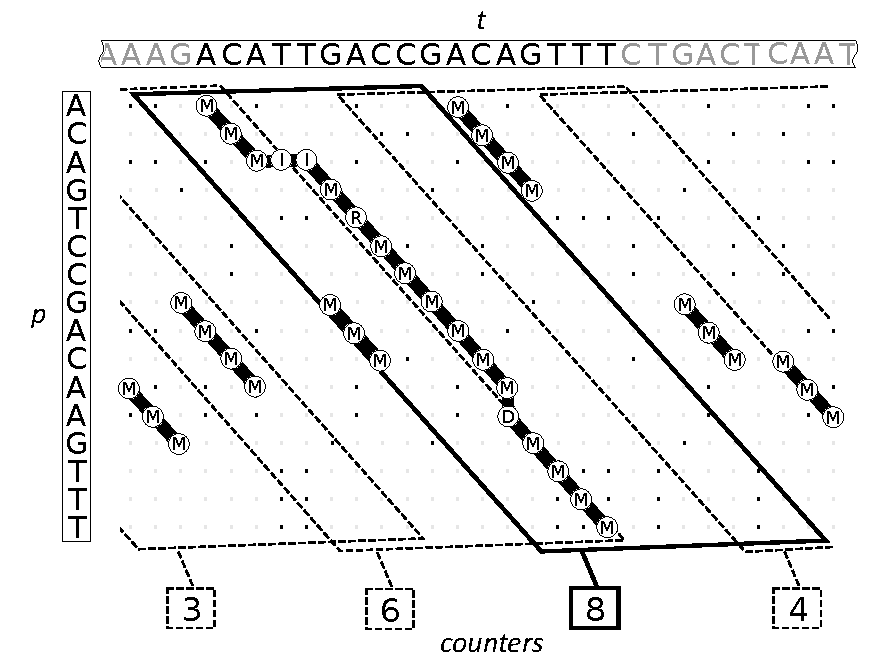
\includegraphics[scale=0.75]{figures/swift.pdf}
\end{center}
\end{figure}

This method lends itself to work in a multiple online fashion rather than offline.
The filtration stage scans the text and counts how many $q$-grams of the pattern fall into each bucket.
The verification stage then verifies only parallelograms exceeding threshold $\tau_q(m,k)$.
As long as the filter scans the text, such implementation remembers only buckets covering the patterns' lengths.
To speed up the filtration phase, an index of the text could be used to count the $q$-gram.
However, this implementation would require more memory, both to keep the text index in memory and to bucket the whole text.

\subsection{Parameterization}

Which is the biggest $q$-gram length yielding lossless filtration given $m$ and $k$?
In order to satisfy lemma~\ref{lemma:qgrams}, the $q$-gram threshold must be greater than zero, \ie it must hold $\tau_q(m,k) \geq 1$.
Thus, by substituting $\tau$, it follows that the $q$-gram length must be $q \leq \left \lfloor \frac{m}{k+1} \right \rfloor$, analogously to equation~\ref{eq:seed-len} of seed filters.
%However, a threshold of 1 does not make filtration very specific.

% -----------------------------------------------------------------------------

\section{Gapped $q$-grams}
\label{sec:filtering:qgrams-gapped}

The idea of \emph{gapped $q$-grams} is to lower the correlation between consecutive $q$-grams.
The occurrence of any contiguous $q$-gram is strongly correlated to the occurrences of its preceding and following $q$-grams.
One single edit distance error affects a cluster of $q$ consecutive $q$-grams, as evidenced by the $q$-gram lemma.
Gapped $q$-grams hence define patterns of \emph{don't care positions} to skip characters at fixed positions.
Such don't care positions are immune to mismatches but not to insertions and deletions.
Hence, this generalization of contiguous $q$-grams is useful to solve $k$-mismatches but not $k$-differences.
%Filtration specificity increases either by raising the filtering threshold or the $q$-gram length, in either cases preserving full-sensitivity.

Gapped $q$-grams rely on a generalization of the $q$-gram similarity measure (section~\ref{sec:filtering:qgrams-ext}) to \emph{subsequences}.
A subsequence is a non-contiguous sequence of symbols of a given string.
Hence, instead of substrings, filtration with gapped $q$-grams counts the number of subsequences of length $q$ common to two strings, whose positions are taken from a fixed set $Q$.
The formal definition of gapped $q$-gram follows.

\begin{definition}
A $Q$-gram is a finite sequence $Q$ of natural numbers starting with the unit element, \ie $Q \subset \N$ and $1 \in Q$.
The cardinality $|Q|$ is called the \emph{weight} of $Q$ and denoted as $w(Q)$.
The maximum element of $Q$ is named \emph{span} and indicated by $s(Q)$.
\end{definition}
%In literature, $Q$-grams are visualized as words over the alphabet $\{1,*\}$ or $\{\#,-\}$.
%I adopt the former notation and represent the $Q$-gram by the word $w \in \{1,*\}^{s(Q)}$ such that $w_j=1$ iff $j \in Q$.

\begin{figure}[h]
\begin{center}
\caption[Filtration with gapped $q$-grams]{Filtration with gapped $q$-grams.}
\label{fig:qgrams-gapped}
\begin{tikzpicture}[font=\normalsize\sffamily]

\transcript{25}{G/1/G, C/1/C, T/1/T, T/1/T, N/0/A, G/1/G, T/1/T, G/1/G, C/1/C, G/0/A, T/1/T, A/1/A, T/1/T, T/1/T, A/0/G, A/1/A, G/1/C, C/1/C, C/1/C, G/0/A, T/1/T, T/1/T, A/0/T, A/1/A, T/1/T}{5}
\band{25}
\seed{1}{25}{1}

\node[left=0.25cm of read_1] {$\Pattern$} ;
\node[left=0.25cm of genome_1] {$\Text$} ;

% Unaffected q-grams ###-#
\foreach \x in {4,9,14}
{
	\pgfmathtruncatemacro{\y}{1+Mod(\x-1,5)}
	\qgramg{\x}{$\#$, $ $, $\#$, $\#$, $\#$}{\y}{1}
}

% Covered q-grams ###-#
\foreach \x in {1,2,3,5,6,7,8,10,11,12,13,15,16,17,18,19,20,21}
{
	\pgfmathtruncatemacro{\y}{1+Mod(\x-1,5)}
	\qgramg{\x}{$\#$, $ $, $\#$, $\#$, $\#$}{\y}{0}
}

% Strikes over covered q-grams
\foreach \x in {1,2,3,5,6,7,8,10,11,12,13,15,16,17,18,20}
{
	\pgfmathtruncatemacro{\y}{5-Mod(\x-1,5)}
	\draw[strike] (qgram_\x_\y.north) -- (qgram_\x_\y.south) ;
}
\draw[strike] (qgram_21_3.north) -- (qgram_21_3.south) ;
\draw[strike] (qgram_20_4.north) -- (qgram_20_4.south) ;
\draw[strike] (qgram_19_5.north) -- (qgram_19_5.south) ;

\end{tikzpicture}
\end{center}
\end{figure}

Figure~\ref{fig:qgrams-gapped} shows an example of $Q$-gram.
As in the $q$-gram lemma, the threshold depends only on $Q$ and parameters $m,k$.
Indeed, the pattern of occurring $q$-grams does not depend on the text or pattern sequences but only on their transcript, \ie on the mismatch positions.
As mismatches do not affect don't care positions, any gapped $Q$-gram potentially yields a higher threshold than the contiguous $q$-gram of the same weight.
Unfortunately, the $q$-gram lemma (\ref{lemma:qgrams}) does not give anymore a tight threshold, but only a lower bound.

Gapped $q$-grams raise hard combinatorial questions.
\begin{inparaenum}[(i)]
\item \label{enum:qgram-non-detection} Does a given gapped $q$-gram yield a full-sensitive filter for $k$-mismatches? If so, either
\item \label{enum:qgram-threshold} which is the maximum $q$-gram threshold $t$ that guarantees full-sensitivity? Or alternatively,
\item \label{enum:qgram-error} which is the maximum distance $k$ for which full-sensitivity is guaranteed?
If the answer to question~\ref{enum:qgram-non-detection} is negative and the filter is lossy,
\item \label{enum:qgram-fn} how many false negatives the filter discards?
Considering filtration efficiency,
\item \label{enum:qgram-fp} how many false positives the filter produces?
%If the weight is taken as a simplified criterion predicting filtration efficiency, 
%\item \label{enum:qgram-weight} which is the maximum weight lossless shape?
\end{inparaenum}

Question~\ref{enum:qgram-threshold} has been first considered in \citep{Burkhardt2001,Kucherov2005},
the more general question \ref{enum:qgram-non-detection} has been introduced in \citep{Nicolas2005}, while I consider here for the first time questions \ref{enum:qgram-error}-\ref{enum:qgram-fp}.
With the aim of elucidating these questions, I first introduce simple characteristic functions to formally define transcripts detected by gapped $q$-grams.
Afterwards, I recapitulate known results for questions \ref{enum:qgram-non-detection}-\ref{enum:qgram-fp} and present new exact and approximate solutions.

\subsection{Characteristic functions}

Consider an arbitrary transcript $\sigma$ as a $m$-dimensional vector over $\Bo$, where $|\sigma|_0$ indicates the Hamming distance of the transcript.
Let $\Bo^m_k \subset \Bo^m$ be the set containing all transcripts $\sigma$ such that $|\sigma|_0 = k$.

\begin{definition}
\label{def:qgram-occ}
A $Q$-gram \emph{occurs} at position $i$ in a similarity $\sigma$ iff $\forall j \in Q$ $\sigma_{i+j}=1$.
Fixed a $Q$-gram threshold $t$, the $Q$-gram \emph{detects} $\sigma$ iff it occurs at least $t$ times in $\sigma$.
\end{definition}

\subsubsection{Boolean functions}

Let $T_{Q}^{m}: \Bo^m \rightarrow \Bo$ denote a \emph{boolean function} such that $T_{Q}^{m}(\sigma)$ is true iff the $Q$-gram occurs at least one time in a similarity $\sigma$ of length $m$.
I define such boolean function as the disjunction
\begin{equation}
\label{eq:qgram-bool}
T_{Q}^{m}(\sigma) = \bigvee_{i=1}^{m-s(Q)+1} \bigwedge_{j \in Q} \sigma_{i+j}
\end{equation}
where each \emph{clause} of $T_{Q}^{m}$ represents a single possible occurrence of $Q$ in $\sigma$.
According to definition \ref{def:qgram-occ}, filtration scheme $(Q,t)$ detects $\sigma$ iff $\sigma$ satisfies at least $t$ clauses of $T_{Q}^{m}$.
%The seed boolean function $T_{Q}^{m}$ describes the computation performed by the seed automaton $A_Q$ on all similarities of length $m$.
I define an analogous boolean function for a $Q$-gram family $F$ as the disjunction
\begin{equation}
\label{eq:family-bool}
T_{F}^{m}(\sigma) = \bigvee_{Q_i \in F} T_{Q_i}^{m}(\sigma)
\end{equation}
By definition, $T_{Q}^{m}$ and $T_{F}^{m}$ are \emph{monotone nondecreasing} boolean functions in \emph{disjunctive normal form} (\emph{DNF}).
Since all monotone boolean functions in DNF are minimal, $T_{Q}^{m}$ and $T_{F}^{m}$ are \emph{minimal}.

\subsubsection{Pseudo-boolean functions}

Let the function $t_{Q}^{m}: \Bo^m \rightarrow \N_0$ be the boolean function $T_{Q}^{m}$ acting on $\N_0$.
I define such \emph{pseudo-boolean function} as
\begin{equation}
\label{eq:qgram-pseudo}
t_{Q}^{m}(\sigma) = \sum_{i=1}^{m-s(Q)+1} \prod_{j \in Q}\sigma_{i+j}
\end{equation}
Here $t_{Q}^{m}(\sigma)$ \emph{counts} how many times a $Q$-gram occurs in a similarity $\sigma$ of length $m$.
It is useful to define the complementary function $\bar{t}_{Q}^{m}$, counting how many times a $Q$-gram does not occur in a similarity $\sigma$, as
\begin{equation}
\label{eq:qgram-pseudoneg}
\bar{t}_{Q}^{m}(\sigma) = m - s(Q) + 1 - t_{Q}^{m}(\sigma)
\end{equation}
Analogously, I define a pseudo-boolean function for a $Q$-gram family $F$
\begin{equation}
\label{eq:family-pseudo}
t_{F}^{m}(\sigma) = \sum_{Q_i \in F} t_{Q_i}^{m}(\sigma)
\end{equation}
along with its complementary function
\begin{equation}
\label{eq:family-pseudoneg}
\bar{t}_{F}^{m}(\sigma) = \sum_{Q_i \in F}{(m - s(Q_i) + 1)} - t_{F}^{m}(\sigma)
\end{equation}

The above functions expose important properties which let me devise approximate solutions.
\emph{Nondecreasing monotonicity} of functions $t_{Q}^{m}$ and $t_{F}^{m}$ follow from nondecreasing monotonicity of their boolean counterparts $T_{Q}^{m}$ and $T_{F}^{m}$. Consequently $\bar{t}_{Q}^{m}$ and $\bar{t}_{F}^{m}$ are \emph{monotone nonincreasing}.
From definition~\ref{eq:supermodularity}, function $t_{Q}^{m}$ is \emph{supermodular}, thus it follows that $\bar{t}_{Q}^{m}$ is \emph{submodular}.
Since super and submodular functions are closed under non-negative linear combination, functions $t_{F}^{m}$ and $\bar{t}_{F}^{m}$ are respectively super and submodular.

\subsection{Full-sensitivity}

\textsc{Non Detection}~\citep{Nicolas2005}. Does a given $Q$-gram yield a full-sensitive filter for $k$-mismatches?

\subsubsection{Problem definition}

\paragraph{}
\begin{tabular}{rl}
{\bf Instance}	&	A $Q$-gram, two integers $m,k$ with $0 < k < m$. \\
{\bf Question}	&	Does it exist a similarity $\sigma \in \Bo^{m}_{k}$ such that $T_{Q}^{m}(\sigma)$ is false? \\
\end{tabular}
\\

\subsubsection{Hardness results}

\textsc{Non Detection} is \emph{strongly} NP-complete \citep{Nicolas2005}.
\citeauthor{Nicolas2005} introduce an intermediate problem, called \textsc{Soapy Set Cover}. They reduce \textsc{Exact Cover by 3-Sets} to \textsc{Soapy Set Cover} and \textsc{Soapy Set Cover} to \textsc{Non Detection}.
Strong NP-completeness implies that no \emph{FPTAS} nor any \emph{pseudo-polynomial} algorithm for it exist, under the assumption that $P \neq NP$.


\subsection{Optimal threshold}

Which is the highest $Q$-gram threshold $t$ that guarantees full-sensitivity?
This problem has been introduced in \citep{Burkhardt2001}. %and generalized in \citep{Kucherov2005}.

\subsubsection{Problem definition}

\paragraph{}
\begin{tabular}{rl}
{\bf Instance}	&	A $Q$-gram, two integers $m,k$ such that $0 < k < m$.\\
{\bf Solution}	&	The largest integer $t^*$ such that \textsc{Non Detection} for $(Q,t^*),m,k$ answers \emph{no}.\\
\end{tabular}
\\

Recalling $Q$-gram pseudo-boolean functions \ref{eq:qgram-pseudo}, I can define the optimal threshold problem as the minimization of a supermodular function subject to linear constraints
\begin{equation}
\begin{array}{ll}
\min & t_{Q}^{m} (\sigma)			\\
w.r.t.								\\
& \sigma \in \Bo^m_k				\\
\end{array}
\end{equation}

\subsubsection{Exact DP solution}

Optimal threshold is fixed-parameter tractable (FPT) in the span of the $q$-gram shape.
\citeauthor{Burkhardt2001} give a DP algorithm computing the optimal threshold in time $O(m \cdot k \cdot 2^{s(Q)})$ \citep{Burkhardt2001}.
\citeauthor{Kucherov2005} give an extension for $Q$-gram families \citep{Kucherov2005}.

%All possible assignments, \ie $\Bo^s(Q)$, for the first clause $\bigwedge_{j \in Q}{\sigma_j}$ of the boolean function $T_{Q}^{m}$ are considered and all satisfying assignments for it, \ie $\phi(Q)$, are computed.
%Clause $Q_2$ is considered next...

\subsubsection{Exact ILP solution}

I reduce this problem to \emph{maximum coverage} \citep{Vazirani2001} and solve it with the following ILP
\begin{equation}
\begin{array}{ll}
\max & |c|_1					\\
w.r.t.							\\
& \sigma \in \Bo^m_k			\\
& c \in \Bo^{m - s(Q) + 1}		\\
& \sigma_i \geq c_j				\\
\end{array}
\end{equation}
where variable $c_j$ indicates the truthfulness of the $j$-th clause in $T_{Q}^{m}$.
The optimal threshold $t^* = |c^*|_1$ is then obtained from the ILP solution $c^*$.

\subsubsection{APX solution}

I reduce the complementary optimal threshold problem to the maximization of a submodular function subject to linear constraints
\begin{equation}
\begin{array}{ll}
\max & \bar{t}_{Q}^{m}(\sigma)		\\
w.r.t.								\\
& \sigma \in \bar{\Bo}^m_k			\\
\end{array}
\end{equation}
where the complementary optimal threshold is $\bar{t}^* = m - s(Q) + 1 - t^*$.

I compute an approximate solution via deepest descent.
My greedy algorithm for complementary \textsc{Optimal Threshold} has an APX-ratio of $1 + 1/e$ \citep{Vazirani2001}.
The same \emph{absolute error} applies to \textsc{Optimal Threshold}.

\subsection{Maximum error}

Which is the maximum error $k^*$ for which full-sensitivity is guaranteed?

\subsubsection{Problem definition}

\paragraph{}
\begin{tabular}{rl}
{\bf Instance}	&	A $Q$-gram, an integer $m > 0$.\\
{\bf Solution}	&	The largest integer $k^*$ such that \textsc{Non Detection} for $Q,m,k^*$ answers \emph{no}.\\
\end{tabular}
\\

Recalling pseudo-boolean functions \ref{eq:qgram-pseudo}, I define this problem as the minimization of a linear function subject to submodular constraints
\begin{equation}
\begin{array}{ll}
\min & |\sigma|_1			\\
w.r.t.								\\
& \sigma \in \Bo^m					\\
& \bar{t}_{Q}^{m}(\sigma) \leq 0	\\
\end{array}
\end{equation}

\subsubsection{ILP solution}

I reduce the problem to \textsc{Minimum Set Cover} \citep{Vazirani2001}, solve it with the following ILP
\begin{equation}
\begin{array}{ll}
\min & |\sigma|_1	\\
w.r.t.				\\
& \sigma \in \Bo^m	\\
& b \in \Bo^{m-s(Q)+1}\\
& A\sigma \geq b	\\
\end{array}
\end{equation}
where the value $A_{ij}$ of the coefficient matrix $A$ is defined as
\begin{equation}
A_{ij} = 
\left\{
	\begin{array}{ll}
		1  & \mbox{if } i-j+1 \in Q		\\
		0  & \mbox{if } i-j+1 \notin Q	\\
	\end{array}
\right.
\end{equation}
and find the maximum error for which full-sensitivity is guaranteed as $k^* = |\bar{\sigma}^*|_1$ given the solution $\sigma^*$ to the ILP.

Contiguous $q$-grams provide an interesting special case of this ILP.
If $A$ has the \emph{consecutive ones property}, it is \emph{totally unimodular}.
The \emph{polytope} defined by a totally unimodular coefficient matrix is \emph{integral}.
Hence the optimal solution of the relaxed LP is also the optimal solution of the original ILP.


\subsubsection{APX solution}

Again, I compute an approximate solution via deepest descent.
APX-ratio of $H_{w(Q)}$ \citep{Vazirani2001}.


\subsection{Specificity}

How many false positives the filter produces?

\subsubsection{Problem definition}

\paragraph{}
\begin{tabular}{rl}
{\bf Instance}	&	A $Q$-gram, two integers $m,k$ such that $0 < k < m$.\\
{\bf Solution}	&	The number of false positives produced by the $Q$-gram.\\
\end{tabular}
\\

False positives are true points of the boolean function \ref{eq:qgram-bool} which have weight inferior to $m-k$ and satisfy more than $t$ clauses of $T_{Q^t}^{m}$.
Hence, I define the function $\text{FP}_{k}^{m}$ counting the number of false positives of filter $(Q,t)$ in instance $(m,k)$ as
\begin{equation}
\text{FP}_{k}^{m}(Q,t) = \sum_{\sigma \in {\bar{\Bo}^{m}_{k}}} T_{Q,t}^{m}(\sigma)
\end{equation}

\subsubsection{FPRAS solution}

I reduce counting false positive transcripts to counting the number of true assignments of a boolean function in DNF.
\citeauthor{Karp1989} introduce a \emph{fully polynomial-time randomized approximation scheme} (FPRAS) to count the number of true assignments of a DNF \citep{Karp1989}.
This method is importance sampling \citep{Vazirani2001}.

%\subsection{Sensitivity and specificity}
%and \ref{enum:qgram-fn}.

%\subsection{Optimal gapped $q$-grams}
%
%Introduced in \citep{Nicolas2005}.
%
%\subsubsection{Problem definition}
%
%\paragraph{}
%\begin{tabular}{rl}
%{\bf Instance}	&	A finite set $S$ of similarities.\\
%{\bf Solution}	&	A $Q$-gram that detects all similarities of $S$.\\
%{\bf Measure}	&	The weight $w(Q)$ of the $Q$-gram.\\
%\end{tabular}
%\\
%
%Given a set of similarities, find the $Q$-gram of maximum weight detecting all similarities.
%This applies to the DNA Homology Search Framework as well.
%%The MWLS is not the optimal seed for approximate string matching filtration nor for sequence homology filtration.
%%On the one hand the weight is just an estimator of sensibility regardless of threshold, on the other hand filtration speed decreases with increasing weight.
%
%\subsubsection{Hardness and inapproximability results}
%
%Nicolas et al. \citep{Nicolas2005} perform an approximation preserving reduction from \textsc{Maximum Independent Set}.
%MWLS is NP-hard and APX-hard within $(|S|)^{0.25 - \epsilon}$ unless $P = NP$.
%If $S = \Bo^{m}_{k}$, $|S| = \binom{m}{k}$.
%
%\subsubsection{Branch-and-bound search}
%
%Burkhardt et al. \citep{Burkhardt2001} bounding criterion. If $Q_1 \subseteq Q_2$, then $t_{Q_2}(m,k) \leq t_{Q_1}(m,k)$.
%Such bounding criterion allows to discard parts of the search space which do not solve the considered $(m,k)$ instance.
%%The search space of seed families is more dense than the search space of single seeds (i.e. almost all seed families solve a give Non Detection instance). Thus search space pruning would not be as effective.

% -----------------------------------------------------------------------------

%\section{Verification methods}
%\label{sec:verification}
%\section{Myers' bit-vector algorithm}
%\subsection{Banded Myers' bit-vector algorithm}
%\subsection{Increased bit-parallelism using SIMD instructions}

\ifthenelse{\boolean{noskeleton}}{}{\clearemptydoublepage}

% === Read Mapping =====================================================================

\ifthenelse{\boolean{noskeleton}}{}{\part{Read Mapping}}

% =============================================================================

\chapter{Background}

Next generation sequencing is a terrific technology.
A wealth of applications have been developed on top of it.
Data analysis pipelines for variant calling and structural variation discovery from DNA-seq, mRNA transcripts abundance estimation and novel non-coding RNA discovery from RNA-seq, transcription factor binding-sites prediction from ChIP-seq.
All these applications rely on a common prerequisite step: mapping NGS reads to a known reference genome.

Read mapping is a critical step in all NGS data analysis pipelines.
NGS reads produced by all current technologies contain sequencing errors, in form of single miscalled bases or stretches of oligonucleotides.
Moreover, the donor genome from which reads have been sequenced contains small genomic variations (SNVs, Indels) in addition to CNV, inversions and translocations.
After all, spotting genomic variation is one reason for which we resequence genomes.
Thus, when mapping a read to a reference genome, it is not sufficient to consider the loci where the reads map exactly; it is necessary to consider any loci of relevant sequence similarity, being possible origins of the sequenced reads.

\section{Sequencing technologies}

\subsection{Illumina}
Illumina / Solexa.

\subsection{Ion Torrent}
Life Technologies / Ion Torrent.

\subsection{454 Life Sciences}
Roche / 454 Life Sciences.

%\subsection{SOLiD}
%ABI / SOLiD.

\section{Sequencing protocols and applications}

\subsection{DNA-seq}
\subsection{RNA-seq}
\subsection{ChIP-seq}

\section{Sequencing quality}

%\subsection{Phred base quality values}

Phred base quality values have been introduced in \citep{Ewing1998, Ewing1998b} to assess the quality of sequencing single bases in capillary reads.
Instead of directly discarding low-quality regions present in capillary reads, Phred calls each base and annotates it with a quality score encoding the probability that it has been wrongly called.
As this method has been widely accepted, base callers annotate reads issue of all sequencing technologies with Phred base quality scores.

To formally define Phred base quality values, let us fix the alphabet $\Sigma = \{$~A,~C,~G,~T~$\}$, and consider a known donor genome $g$ over $\Sigma$ and a read $r$ sequenced at location $l$ from the template $g_{l \dots l+|r|-1}$.
We define the base calling error $\epsilon_i$ at position $i$ in the read $r$, as the probability $\epsilon_i$ of miscalling a base $r_i$ instead of calling its corresponding base $g_{l+i-1}$ in the donor genome.
Therefore, we define the Phred base quality $Q_i$ at position $i$ as:
\begin{eqnarray}
Q_i = -10 \log_{10} \epsilon_i.
\end{eqnarray}

Given the above, the probability $p(r_i | g_{l+i-1})$ of calling the base $r_i$ in the read $r$, given the donor genome base $g_{l+i-1}$, is:
\begin{eqnarray}
p(r_i | g_{l+i-1}) = \left\{
\begin{array}{ll}
1-\epsilon_i                  & \text{ if } g_{l+i-1} = r_i\\
\frac{\epsilon_i}{|\Sigma|-1} & \text{ if } g_{l+i-1} \in \Sigma \setminus \{r_i\}\\
\end{array}
\right.
\end{eqnarray}
and assuming \iid base calling errors, it follows that the probability $p(r | g, l)$ of observing the read $r$, given the donor genome template $g_{l \dots l+|r|-1}$, is:
\begin{eqnarray}
\label{eq:phred}
p(r | g, l) = \prod_{i=1}^{|r|}{p(r_i | g_{l+i-1})}
\end{eqnarray}

% =============================================================================

\section{Mappability}
\label{sec:mappability}

Genome resequencing is a non-trivial task.

The difficulty of unambiguously finding the correct mapping location of next-generation sequencing reads comes from the non-random nature of genomes.
Genomes evolved through multiple types of duplication events, including
\begin{inparaenum}[(i)]
\item whole-genome duplications \citep{?} or large-scale segmental duplications in chromosomes \citep{?},
\item transposition of repetitive elements as short tandem repeats (microsatellites) and interspersed nuclear elements (LINE, SINE) \citep{?},
\item proliferation of repetitive structural elements such as telomeres and centromeres \citep{?}.
\end{inparaenum}
As a result of these events, about 50~\% of the human genome is composed of repeats.

An analysis of the $k$-mer spectra of the genomes of some model organisms shows how genomes are statistically different from texts randomly generated according to uniform bernoulli models.

Repeats present in general technical challenges for all \emph{de novo} assembly and sequence alignment programs \citep{Lee2012}.
In the case of short reads mapping, the first evident effect of the heavy tail in the $k$-mer distribution of reference genomes is the dramatic loss of specificity in certain regions, which increases the computational cost of programs based on filtration methods.
But the most subtle challenge lies in the interpretation of these results: it is not evident how to consider reads mapping to multiple locations.

Common strategies to deal with multi-reads are
\begin{inparaenum}[(i)]
\item to discard them all,
\item to randomly pick one best mapping location,
\item to consider all or up to $k$ best mapping locations within a given distance threshold
\end{inparaenum}
\citep{Treangen2011}.

A practical challenge is represented by reporting and handling the resulting datasets of mapping locations, which can have a size up to two orders of magnitude bigger compared to the corresponding input read sets.

Genome mappability can bias NGS analysis more than we might think at a first glance.
Two recent studies \citep{Derrien2012, Lee2012} show which is the bias of mappability.


% -----------------------------------------------------------------------------

\subsection{Genome mappability}

We now give a definition of genome mappability analogous to \citep{Derrien2012}.
Let fix a $q$-gram length, a distance measure as the Hamming or edit distance, and a distance threshold $k$.
Given a genomic sequence $g$, we define the $(q,k)$-frequency $F^q_k(l)$ of the $q$-gram $g_{l \dots l+q-1}$ at location $l$ in $g$ as the number of occurrences of the $q$-gram in $g$ and its reverse complement $\bar{g}$.
We define the $(q,k)$-mappability $M^q_k(l)$ as the inverse $(q,k)$-frequency, \ie $M^q_k(l) = {F^q_k(l)}^{-1}$ with $M^q_k : \N \rightarrow ]0,1]$.
Note that $M^q_k(l)$ can be seen as the prior probability that any read of length $q$ originating at location $l$ will be mapped correctly.
The values of $(q,k)$-frequency and mappability obviously vary with the distance threshold $k$. Nonetheless, under any distance measure, it hold that the $q$-gram at location $l$ is unique up to distance $k$ iff $M^q_k(l) = 1$ and repeated otherwise.

Which is the minimum $q$-gram length from which we expect $(q,k)$-mappability to be $1$ for the genomes of model organisms?
Let consider the simple case of exact $(q,0)$-mappability.
By assuming a genomic sequence of length $n$ as being randomly generated under the uniform bernoulli model, the emission probability of any nucleotide is $p=\frac{1}{4}$ and, under \iid assumptions, the emission probability of any $q$-gram is $p_q=\frac{1}{4^q}$.
It follows that the expected value of $(q,0)$-frequency is $E[F^q_0] \simeq \frac{2n}{4^q}$.
Thus, for $E[F^q_0] \leq 1$ it must hold:
\begin{eqnarray}
2n \leq 4^q\\
\log{2n} \leq \log{4^q}\\
q \geq log_{4}{2n}
\end{eqnarray}
Thus, we would expect any $q$-gram of length $\log_{4}2n$ to occur about once in a genomic sequence of length $n$.
Sticking to these assumption, in the human genome ($n \approx 3\cdot10^9$) almost all 17-mers would be unique, on fly ($n \approx 1.2\cdot10^8$) all 15-mers, on worm ($n \approx 4.2\cdot10^7$) all 13-mers.
However, the $q$-gram distribution of model genomes does not fit the uniform bernoulli distribution.
In \citep{?} the $k$-mers distribution can be approximated by a double Pareto log-normal distribution, \ie a distribution with a heavy tail.
This is a result of the evolution of genomes being driven by gene duplications, retrotransposons \citep{?}.


Consequently, we would expect 36~bp reads produced by early Illumina sequencers to induce an almost perfect mappability.
However, reads have to be mapped approximately to the reference genome.
The expected number of approximate occurrences of a $k$-mer is higher than the exact one.
Thus the above estimate is a lower bound.

\subsubsection{Uniqueome}

\citeauthor{Derrien2012} quantified the whole genome unique mappability for human, mouse, fly, and worm.
At a $(36,2)$ mapping, about 30~\% of the human genome is not uniquely mappable.
Unique mappability rises to 83~\% by increasing the read length to 75~bp; however to map a significant fraction of the reads, we should consider 3--4 edit distance errors.

\begin{table}[h]
\begin{center}
\caption[Mappability]{Mappability of model genomes. Data extrapolated from \citep{Derrien2012}.}
\sffamily
    \begin{tabular}{lccc}
    \toprule
    ~                                        & H.sapiens & M.musculus & D.mel \\
    ~                                        & (hg19) & (mm9) & (dm3) \\
    \midrule
    Repeats content [\%]               & 45.25            & 42.33            & 26.50      \\
    \midrule
%    Uniqueome (36,0) [\%]               & 80.12            & 79.92            & 26.50      \\
%    Uniqueome (50,0) [\%]               & 45.25            & 42.33            & 26.50      \\
%    Uniqueome (75,0) [\%]               & 45.25            & 42.33            & 26.50      \\
%    \midrule
    Uniqueome (36~bp, 2~msm) [\%]               & 69.99            & 72.07            & 68.09      \\
    Uniqueome (50~bp, 2~msm) [\%]               & 76.59            & 77.06            & 69.44      \\
    Uniqueome (75~bp, 2~msm) [\%]               & 83.09            & 81.65            & 71.00      \\
    \bottomrule
    \end{tabular}

\end{center}
\end{table}

The uniqueome plays an important role in ChIP-seq experiments.
It is common practice \citep{?} to rely on short (36~bp) reads and discard the non-unique ones.
Not only a significant fraction of the sequencing data is thrown out.
Worse than that, we end up with holes in 30~\% of the genome.
A ChIP-seq peak caller considering multi-reads calls up to 30~\% more peaks.

Cite regions of clinical relevance, \eg HLA-A.
Cite regions of biological relevance, \eg 5S rRNA.

\subsubsection{Paired-end mappability}

\subsubsection{Pileup mappability}

If we focus our attention to the resequencing accuracy at a single locus, we have to consider the mappability of all the possible reads spanning that given locus.
Pileup mappability \citep{Derrien2012} at position $i$ is the average mappability of all reads spanning position $i$.

$M_p(i) = 1/q \sum_{j=i}^{i+1}{M(j)}$


\subsection{Mapping quality score}
\label{sub:mapqual}

Mapping quality has been introduced in \citep{Li2008}.
The study considers short reads of length ranging from 30~bp to 40~bp, produced by early Illumina/Solexa and ABI/SOLiD sequencing technologies, whose sequencing error rates were quite high.
Given the short lengths and high error rates, a significant fraction of such reads can be aligned to multiple mapping locations, even considering only co-optimal Hamming distance locations.

The key point is that the Hamming distance is not an adequate scoring scheme to guess the correct mapping location of many reads.
The authors claim\footnote{\citeauthor{Li2008} do not show in their study what is the effect of relying on mapping quality rather than on mapping uniqueness.} that:
\begin{quote}It is possible to act conservatively by discarding reads that map ambiguously at some level, but this leaves no information in the repetitive regions and it also discards data, reducing coverage in an uneven fashion, which may complicate the calculation of coverage.\end{quote}
Since base callers output base call probabilities in Phred-scale along with the reads, \citeauthor{Li2008} propose a novel probabilistic scoring scheme called mapping quality, giving the probability that a given read has been aligned correctly at a given mapping location in the reference genome.

By applying Bayes' theorem, we can derive the posterior probability $p(l|g,r)$, that location $l$ in the reference genome $g$ is the correct mapping location of read $r$.
Assuming uniform coverage, each location $l \in [1, |g| - |r| + 1]$ has equal probability of being the origin of a read in the donor genome, thus the prior probability $p(l)$ is simply:
\begin{eqnarray}
p(l) = \frac{1}{|g| - |r| + 1}
\end{eqnarray}
Therefore, recalling $p(r | g, l)$ from equation~\ref{eq:phred}, the posterior probability $p(l|g,r)$ equals the probability of the read $r$ originating at location $l$ normalized over all possible locations in the reference genome:
\begin{eqnarray}
\label{eq:mapprob}
p(l|g,r) = \frac{p(r|g,l)}{\sum_{i=1}^{|g| - |r| + 1}{p(r|g,i)}}
\end{eqnarray}
which in Phred-scale becomes:
\begin{eqnarray}
\label{eq:mapqual}
Q(l|g,r) = -10 \log_{10}[1 - p(l|g,r)]
\end{eqnarray}

Computing the exact mapping quality as in equation~\ref{eq:mapqual} requires aligning each read to all positions in the reference genome.
On one hand, this computation would not be practical, indeed the vast majority of a reference genome is discarded when mapping reads by means of filtering and fully-indexed methods.
On the other hand, the contribution of discarded locations to the sum in equation~\ref{eq:mapprob} can be neglected.
Therefore, equation~\ref{eq:mapprob} is approximated using only relevant mapping locations found by the read mapper.

Mapping quality has been initially used in \citep{Li2008} and \citep{Li2009} to maximize variant calling confidence by discarding reads whose best mapping location is below a given mapping quality threshold.
This measure has been widely accepted: nowadays it is computed by most popular read mappers and used by almost all variant calling pipelines \eg the Genome Analysis ToolKit (GATK) \citep{DePristo2011}.

Nonetheless, some important objections can be moved against mapping quality.
First, the mapping quality score is derived under the unlikely assumption of the reference genome being equal to the donor genome.
In other words, mapping quality considers only errors due to base miscalls and disregards genetic variation; thus the risk is to prefer mapping locations supported by known low base qualities rather than by true but unknown SNVs.
Second, mapping quality is nonetheless strongly correlated to mapping uniqueness, as discussed in section~\ref{sec:mappability}; it is easy to see that the mapping probability in equation~\ref{eq:mapprob} is diluted in presence of a large number of co-optimal mapping locations.
Third, mapping quality tends to become less relevant as base calls improve, due to advances of sequencing technologies, and thus degenerates in a shallow measure of uniqueness.

\subsection{Genome mappability score}

Genome mappability score (GMS) \citep{Lee2012} is analogous to pileup mappability.
Instead of considering the inverse mapping frequency $(q,k)$-mappability, we can interpret mapping quality (see subsection~\ref{sub:mapqual}) as the probability that a read originating at a given position can be mapped correctly. %which is effectively a probabilistic mappability measure,
Therefore, we consider the average mapping probability of any read spanning a location $l$ of a reference genome $g$\footnote{Equation~3 in \citep{Lee2012} is not precise, please refer to our equation~\ref{eq:gms}.}:
\begin{eqnarray}
\label{eq:gms}
p(l|g) = \sum_{r \in \mathcal{R}(l)}{\frac{p(l|g,r)}{|\mathcal{R}(l)|}}
\end{eqnarray}
which in Phread-scale becomes:
\begin{eqnarray}
Q(l|g) = \sum_{r \in \mathcal{R}(l)}{\frac{1 - 10^{-\frac{Q(l|g,r)}{10}}}{|\mathcal{R}(l)|}}
\end{eqnarray}
and thus, fixed a genomic sequence $g$, we define the genome mappability score $\text{GMS}(l)$ as its percentual value:
\begin{eqnarray}
\text{GMS}(l) = 100 Q(l|g)
\end{eqnarray}

\citeauthor{Lee2012} simulate reads having length and error profiles similar to those issue by actual sequencing technologies, define low GMS regions as those locations for which $\text{GMS}(l) \leq 10$, and measure the percentage of such locations in the human genome.

\begin{table}[h]
\begin{center}
\caption[Genome mappability score]{Human genome mappability score of various sequencing technologies. Data extrapolated from \citep{Lee2012}.}
\sffamily
    \begin{tabular}{lrrrr}
    \toprule
    Sequencing                 & Read length   & Error rate & Low GMS          & High GMS \\
    technology                 & [bp]          & [\%] (msm, ins, del) & [\%]             & [\%] \\
    \midrule
%    SOLiD-like                 & 75            & (0.10, 0.00, 0.00) & 11.14            & 88.86      \\
    Illumina-like              & 100           & (0.10, 0.00, 0.00) & 10.51            & 89.49      \\
    Ion Torrent-like           & 200           & (0.04, 0.01, 0.95) & 9.35  & 90.65      \\
    Roche/454-like             & 800           & (0.18, 0.54, 0.36) & 8.91  & 91.09      \\
%	PacBio-like                & 2000          & (1.40, 11.47, 3.43) & 100.0            & 0.00      \\
	PacBio EC-like             & 2000          & (0.33, 0.33, 0.33) & 8.61  & 91.39      \\
    \bottomrule
    \end{tabular}
\end{center}
\end{table}

% =============================================================================


\section{Popular read mappers}

Critic the surveys classifying hundreds of mappers \citep{Li2010}, \citep{Fonseca2012}.

Critic the benchmarks \citep{Hatem2013} \citep{Holtgrewe2011}.

The task of a read mapper is to guess where a read originates.
Fixed a similarity scoring scheme that confidently models this problem, the optimal alignment under this scoring scheme correspond to the most likely explanation and induces a locus being the origin of the read.
The simplest scoring scheme is the edit distance; more involved scoring schemes take into account base quality values, score gaps using affine cost functions, or allow to trim for free a prefix or a suffix of the read.

The above definition does not consider two problems: what if there are many co-optimal candidates, and what if the correct solution corresponds to a sub-optimal candidate.
The former problem is exacerbated by genome mappability.
One would expect such situations to arise very rarely, but instead it is a relevant problem.
The latter problem arises whenever our model is not adequate to explain the difference between a read and its genomic origin.
For instance, an evolutionary event producing an indel of length $l$ might be considered as a unit, whether edit distance would consider it as $l$ independent events.
Under the edit distance, an alignment with less than $l$ independent point mutations would be considered more likely than an alignment containing only one indel of length $l$.

From the former problem, we conclude that considering only one optimal mapping location is not sufficient, no matter how good our scoring scheme can be.
The latter problem tells us to be careful about relying on strict optimality.
Therefore, in general a read mapper should return a comprehensive set of relevant mapping locations along with the likelihood that they correspond to the original location.

% -----------------------------------------------------------------------------

\subsection{Bowtie}

Bowtie \citep{Bowtie} is a mapper designed to have a small memory footprint and quickly report a few good mapping locations for early generation Illumina/Solexa and ABI/SOLiD short reads of length up to 50~bp.
It achieves the former goal by indexing the reference genome with an FM-index and the latter goal by performing a greedy depth-first traversal on it.

The greedy depth-first traversal visits first the subtree yielding the least number of mismatches and stops after having found a candidate (not guaranteed to be optimal when $k>1$).
In addition, Bowtie speeds up backtracking by applying case pruning, a simple application of the pigeonhole principle.
However this technique is mostly suited for $k=1$ and requires the index of the forward and reverse text.

Bowtie can be configured to search by strata, however the search time increases significantly while the traversal still misses a large fraction of the search space due to seeding heuristics.
Main practical drawbacks of the tool are too many cryptic options.

Bowtie~2 \citep{Bowtie2} has been designed to quickly report a couple of mapping locations for recent Illumina/Solexa, Ion Torrent and Roche/454 reads, usually having lengths in the range from 100~bp to 400~bp.

This tool uses an heuristic seed-and-extend approach, collecting seeds of fixed length, partially overlapping, and searching them exactly in the reference genome using an FM-index.
Candidate locations to verify are chosen randomly, to avoid uncompressing large CSA intervals and executing many DP instances.
Each mapping location is verified using a striped vectorial dynamic programming algorithm, implemented using SIMD instructions, previously introduced by \citep{Farrar2007} and extended to compute end-to-end alignments.

Bowtie~2 can be configured to report end-to-end or local alignments, scored using a tunable affine scoring scheme.
For this reason, it is believed to be good at reporting alignments containing indels.
However, its completely heuristic filtration strategy, independent of the scoring scheme, makes it hard to believe what it promises.

% -----------------------------------------------------------------------------

\subsection{BWA}

BWA-backtrack \citep{BWA} is designed to map Illumina/Solexa reads up to 100~bp and report a few best end-to-end alignments.
The program performs a greedy breadth-first search on an FM-index of the reference genome.
Nodes to be visited are ranked by edit distance score: the best node is popped from a priority queue and visited, its children are then inserted again in the queue.
The traversal considers indels using a more involved 9-fold recursion.
Backtracking is sped up by adopting a more stringent pruning strategy that nonetheless takes some preprocessing time and requires the index of the reverse reference genome.

BWA performs paired-end alignments by trying to anchor both paired-end reads and verifying the corresponding mate, within an estimated insert size, using the classic DP-based Smith-Waterman algorithm.
Consequently, the program in paired-end mode aligns reads at a slower rate than in single-end mode.
The program is not fully multi-threaded, therefore BWA scales poorly on modern multi-core machines.

BWA-SW \citep{BWA-SW} is designed to map Roche/454 reads, which have an average length of 400~bp.
It is an heuristic version of BWT-SW, designed to report a few good local alignments.

This version of BWA adopts a double indexing strategy: it indexes all substrings of one read in a DAWG.
It performs Smith-Waterman of all read substrings directly on the FM-index, by backtracking as soon as no viable alignment can be obtained.
As in BWA-backtrack, the traversal proceeds in a greedy fashion.
In addition, BWA-SW implements some seeding heuristics to limit backtracking and jump in the reference genome to verify candidate locations whenever this becomes favorable.

This version of BWA does not support paired-end reads, presumably because it was meant for Roche/454 reads.

% -----------------------------------------------------------------------------

\subsection{Soap}

Soap~2 \citep{Soap2} is very similar to Bowtie: it has been designed to produce a very quick but shallow mapping of Illumina/Solexa reads up to 75~bp with no more than 2 mismatches and no indels.
However, its underlying algorithm is based on the so-called bi-directional (or 2-way) BWT.
The tool support paired-end mapping but at a slower alignment rate.
Practical drawbacks are the lack of native output in the de-facto standard SAM format and is closed source.
Soap~3 \citep{Soap3} is algorithmically similar to Soap~2 but targets only NVIDIA CUDA accelerators.

% -----------------------------------------------------------------------------

\subsection{SHRiMP}

SHRiMP~2 TODO.

% -----------------------------------------------------------------------------

\subsection{RazerS}

RazerS \citep{Weese2009} has been designed to report all mapping locations within a fixed hamming or edit distance error rate.
It is based on a full-sensitive $q$-gram filtration method (SWIFT semi-global) combined with the Myers edit distance verification algorithm.
On demand, the SWIFT filter can be configured to become lossy within a fixed loss rate.
The lossy filter becomes more stringent and produces a lower number of candidates to verify, thus improving the overall speed of the program.
All in all, the SWIFT filter is very slow while not highly specific.

RazerS~3 \citep{RazerS3} is a faster version featuring shared-memory parallelism, a faster banded-Myers verification algorithm, and a faster filtration scheme based on exact seeds that however turns out to be very weak on mammal genomes.
Because of this, RazerS~3 is one-two orders of magnitude slower than Bowtie~2 and BWA-backtrack on mammal genomes.

All RazerS versions index the reads and scan the reference genome.
One positive aspect of this strategy is that no preprocessing of the reference genome is required.
However, other mapping strategies beyond all-mapping, \eg mapping by strata, cannot be efficiently implemented.
Moreover, the program exhibit an high memory footprint as it must remember the mapping locations of all input reads until the whole reference genome has been scanned.

% -----------------------------------------------------------------------------

\subsection{mr(s)Fast}

The tools mrFast \citep{Ahmadi2011} and mrsFast \citep{Hach2010} are designed to report all mapping locations within a fixed absolute number errors, respectively under the hamming and edit distance, given Illumina/Solexa reads of length ranging from 50~bp to 125~bp.
Similarly to RazerS~3, they are based on a full-sensitive filtration strategy using exact seeds, which turns out to be very weak on mammal genomes.

The peculiarity of their underlying method is a cache-oblivious strategy to mitigate the high cost of verifying clusters of candidate locations.
In addition, mrsFast computes the edit distance between one read and one mapping location in the reference genome with an antidiagonal-wise vectorial dynamic programming algorithm, implemented using SIMD instructions.

These tools are as slow as RazerS~3 and appealing for nothing more than all-mapping.
They lack multi-threading support and exhibit various bugs.
Furthermore, they only accept reads of fixed length and produce files of impractical size.

% -----------------------------------------------------------------------------

\subsection{GEM}

The GEM mapper \citep{Gem} is a flexible read aligner for Illumina/Solexa, ABI/SOLiD, and Ion Torrent reads.
It is full-sensitive and can be configured either as an all-mapper, as a best/unique-mapper, or to search by strata.

GEM uses a combination of state of the art approximate string matching methods, \eg approximate seeds and suffix filters.
The program indexes the reference genome with an FM-index, tries to find an optimal filtration strategy per read, and verifies candidate locations using Myers algorithm.
Paired-reads are either mapped independently and then combined, or left/right are mapped and their mates verified using an online strategy.

Unfortunately the tool lacks direct SAM output, it is not open source, and provides many obscure parameters.

% -----------------------------------------------------------------------------

\subsection{Masai and Yara}

% -----------------------------------------------------------------------------

\begin{landscape}
\begin{table}[h]
  \center
  \sffamily
%  \resizebox{1.0\textwidth}{!}
%  {
	\renewcommand{\tabcolsep}{0.8ex}
	% latex table generated in R 2.15.0 by xtable 1.7-0 package
% Sun Jul  1 11:47:28 2012
\begin{tabular}{llccccc}
  \toprule 
%  & & \multicolumn{3}{c}{$\overbrace{}^\text{index}$} & \\
   & mapper & { scoring scheme } & {  method } &  { index } & {  reference } & {  reads } \\ 
  \midrule \multirow{4}{*}{\begin{sideways}\scriptsize \hspace{1ex} best\end{sideways}} 
  & {\emph{Masai}} & \emph{edit distance} & \emph{approximate seeds} & \emph{generic} & \cmark & \cmark \\ 
  & {Bowtie\,2} & qualities + affine & exact seeds &  FM-index & \cmark & \xmark \\ 
  & {BWA} & qualities & backtracking & FM-index & \cmark & \xmark \\
%  & {Soap\,2} & qualities & backtracking  & FM-index & \cmark & \xmark \\ 
	  \midrule\multirow{5}{*}{\begin{sideways}\scriptsize \hspace{6ex} all\end{sideways}} 
  & {\emph{Masai}} & \emph{edit distance} & \emph{approximate seeds} & \emph{generic} & \cmark & \cmark \\ 
  & {RazerS\,3 } & edit distance & exact seeds & $q$-gram index & \xmark & \cmark  \\ 
  & {mrFAST } & edit distance & exact seeds & $q$-gram index & \cmark & \cmark \\ 
\bottomrule \end{tabular}

%  }
\end{table}
\end{landscape}

% =============================================================================

\chapter{Masai}

In this chapter we present our first attempt to engineer an efficient all-mapper.
When we started this project, in October 2011, the fastest all-mappers (mrFast and RazerS~3) were two order of magnitude slower than prominent best-mappers (Bowtie and BWA).
On one hand, all-mappers were using filtration based on exact seeds, which is fine for short reference genomes but becomes too weak for mammal genomes; clearly, a stronger filtration strategy would had been beneficial.
On the other hand, best-mappers were based on heuristic backtracking, which was becoming inadequate to map reads of increasing length.
After a thorough literature review, we came out with a novel read mapping method combining seed-based filtering with backtracking.

In the engineering section, we see how our filtration method works, which data structures we adopt for indexing, and how we perform seed extension.
In particular, our filtration method is based on exact or approximate seeds: by employing approximate seeds instead of exact seeds, we obtain a stronger filter for long reference genomes, which is still non-heuristic and quasi full-sensitive.
We find approximate seeds by backtracking the index of the reference genome.
Moreover, we speed up the backtracking phase by searching all seeds simultaneously, with the help of an additional index and the multiple backtracking algorithm.
Lastly, we improve our method to perform best-mapping in a more efficient way.

Our method is packaged in a \CC tool nicknamed \emph{Masai}, which stands for \emph{m}ultiple backtracking of \emph{a}pproximate seeds on a \emph{s}uffix \emph{a}rray \emph{i}ndex.
Masai is part of the SeqAn library, it is distributed under the BSD license and can be downloaded from \url{http://www.seqan.de/projects/masai}.

In the evaluation section, we extensively compare Masai with popular read mappers, both on simulated and real datasets.
Compared to all-mappers mrFast and RazerS~3, Masai is an order of magnitude faster and has comparable sensitivity.
In addition, Masai as a best-mapper is 2--4 times faster and more accurate than Bowtie\,2 \citep{Bowtie2} and BWA \citep{BWA}.

Finally, we discuss the limitations of Masai that led us to engineer Yara, yet another read aligner.

% -----------------------------------------------------------------------------

\section{Engineering}

We start by giving an outline of the read mapping method of Masai.
Later, we give a detailed explanation of each mapping step, explaining and motivating relevant engineering choices that led us to the final implementation.

Masai requires an index capable of simulating a top-down traversal of the suffix trie of the reference genome.
We give to the user the possibility to choose among various indices (see section~\ref{masai:engineering:index}).
Similarly to all read mappers relying on an index of the reference genome, we index the reference genome only once, store it on disk and reuse it for all subsequent read mapping jobs.

At mapping time, Masai requires two parameters to be provided: a maximum number of errors per read and a minimum seed length.
Default parameters work well for actual Illumina reads, otherwise the user has to parametrize adequately the tool for optimal performance.
Nonetheless, independently of the chosen parameterization, filtration is guaranteed to be quasi full-sensitive (see section~\ref{masai:engineering:seeding}).

We partition all reads (and their reverse complements) in non-overlapping seeds;
subsequently we arrange all seeds in a conceptual \emph{trie}.
Using our \emph{multiple backtracking} algorithm, we backtrack simultaneously all indexed seeds in the suffix trie of the reference genome.
We perform seed extension on all hits reported by the multiple backtracking algorithm;
we extend both ends of each seed using a banded version of \emph{Myers bit-vector algorithm} \citep{Myers1999} (details in section~\ref{masai:engineering:extension}).

%In all-mapping, we perform one round of seeding and extension; we immediately write to disk each found mapping location.
%In best-mapping, we perform have to remember one best location per read until we are able to guarantee optimality.

\subsection{Filtration}
\label{masai:engineering:seeding}

%We now consider formally the read mapping problem.
%Given a reference genome $g$, a set of reads $\mathcal{R}$ and an absolute number of errors $k$ consisting of indels and mismatches, for each read $r \in \mathcal{R}$ find all mapping locations where $r$ approximately occurs in $g$ within $k$ errors.

Our original intent was to improve the speed of our all-mapper RazerS \citep{Weese2009}, while preserving full-sensitivity under the edit distance.
RazerS was based on a $q$-gram filter;
we were aware that gapped $q$-grams could have brought a huge speedup, but we could not see any straightforward generalization of gapped $q$-grams to the edit distance.
At the same time, we experienced that weaker but quicker filtration using exact seeds was more advantageous than filtration using $q$-grams (indeed, a typical Illumina read mapping setup requires only moderate error rates, in the range of 4--6~\%).
Thus RazerS~3 \citep{RazerS3} went back to filtration with exact seeds (similarly to mrFast).
Nonetheless, we wanted to improve again filtration specificity, as the runtime of RazerS~3 on mammal genomes became dominated by verifications, and we knew that to improve filtration specificity we had to increase the seed length, as these two things are strongly correlated.

While reviewing past literature in the field of approximate string matching, we rediscovered the works of \citeauthor{Myers1994}, \citeauthor{Navarro2000} on approximate seeds, providing stronger filtration than exact seeds while preserving full-sensitivity under the edit distance.
Their idea is to partition the pattern into $s \leq k+1$ non-overlapping seeds, which obviously can be longer than exact seeds but have to be searched within distance $\lfloor k/s \rfloor$ (see section~\ref{filter:apx}).

Following \citep{Navarro2000}, we decided to find approximate seeds by backtracking the suffix trie of the reference genome (in section~\ref{masai:engineering:index} we recall our engineering work to find approximate seeds efficiently).
For simplicity, we decided to find approximate seeds only under the hamming distance.
For this reason, when resorting to approximate seeds, Masai does not attain strict full-sensitivity under the edit distance.
Nonetheless, in section~\ref{masai:evaluation} we show that such implementation detail sacrifices less than 1\% sensitivity.

Then, we slightly improved the filtration lemma of \citep{Navarro2000}:
we search $(k \bmod{s}) + 1$ seeds within distance $\lfloor k/s \rfloor$ and the remaining seeds within distance $\lfloor k/s \rfloor - 1$.
To prove full-sensitivity it suffices to see that, if none of the seeds occurs within its assigned distance, the total distance must be at least $s \cdot \lfloor k/s \rfloor + (k \bmod s) + 1 = k + 1$.
Hence all approximate occurrences will be found.

Finally, we chose to parameterize our filter by the seed length rather than by the number of seeds.
Clearly, these two parameterization are dual: if we choose the number of seeds to be $s$, the minimum seed length $l$ has to be $\lfloor |r|/s \rfloor$; vice versa, if we fix the minimum seed length to $l$, the number of seeds $s$ has to be $\lfloor |r|/l \rfloor$.
Nonetheless we prefer the latter, as the minimum seed length gives us a direct estimate of the expected number of verifications produced by the filter.
The resulting filter is flexible, indeed by increasing $l$ filtration becomes more specific at the expense of a higher filtration time.

The optimal seed length $l$ depends on the reference genome as well as on read length and the absolute number of errors.
We experimentally evaluated filtration with exact and approximate seeds (see section~\ref{masai:evaluation:filter}).
When mapping current Illumina reads on short to medium length genomes, exact seeds are still more efficient than approximate seeds.
Conversely, on larger genomes (\eg mammalian genomes) approximate seeds outperform exact seeds by an order of magnitude.

\subsubsection{Best-mapping}

Best-mapping asks to report only one of the optimal (any-best) or alternatively all the co-optimal (all-best) mapping locations of any read.
Of course, we can perform all-mapping and then filter out any sub-optimal mapping location.
Here we describe a \emph{greedy} mapping strategy for best-mapping that, in standard read mapping scenarios, is an order of magnitude faster than all-mapping.

Certainly, best-mapping makes sense if the adopted measure is an effective scoring scheme at identifying original mapping locations.
In section~\ref{masai:evaluation:rabema} we see that best-mapping using edit distance is competitive with tools using more complex scoring schemes.


\subsection{Indexing}
\label{masai:engineering:index}

Within the SeqAn library, we initially disposed of two indices capable of simulating a top-down suffix trie traversal: the enhanced suffix array (ESA) \citep{Abouelhoda2004} and the lazy suffix tree (LST) \citep{Giegerich1999}.
To improve the efficiency of Masai, we implemented a generic top-down traversal for some additional indices, namely the suffix array (SA) \citep{Manber1990}, the $q$-gram index, and various flavours of the full-text minute index (FM-index) \citep{Ferragina2001}.
Below we discuss the performance of these indices in our specific application, while we refer the reader to chapter~\ref{chr:index} for their extensive explanation.

\subsubsection{Indexing the reference genome}

We initially chose the ESA over LST because of better construction times.
Indeed, we dispose of a linear time construction algorithm for the ESA (an adaptation of the DC7 algorithm \citep{Dementiev2008} to multiple sequences \citep{Weese2013} for the generalized SA, followed by the algorithms proposed in \citep{Kasai2001,Abouelhoda2004}), while our LST construction algorithm takes quadratic time (using the radix sort based \emph{wotd}-algorithm \citep{Giegerich1999}).
Apart from that, both our ESA and LST implementations require $13$ bytes per base pair and exhibit comparable query speed.
Thus, for the human reference genome (GRCh38), we had a suffix trie constructed in about 1.5~hours and consuming 39~GB of memory (see figure~\ref{fig:index:construction}).

At this point, Masai required high-end hardware to process large reference genomes.
Therefore, thinking of a space-time trade-off, we designed a generic suffix trie top-down traversal for the SA (see section~\ref{sec:index:sa});
indeed, the SA consumes only $5$ bytes per base pair but is theoretically slower than the ESA, as it adds a logarithmic factor to query times.
However, with surprise we found out that, within our application, the SA had equal or better performance than the ESA (see figure~\ref{?}).
Ultimately, we brought down the memory footprint of the index from 39~GB to 15~GB but preserved query speed.

We tried to further improve query speed by removing the logarithmic factor introduced by the SA.
Therefore, to cut the most expensive binary searches, we put a $q$-gram index on top of the SA and extended our generic suffix trie top-down traversal accordingly (see section~\ref{sec:index:qgram}).
Yet, the $q$-gram index did not bring significant speedup to our application;
indeed, the lookup table turned out to be useful when searching patterns one by one, but not when coupled with our multiple backtracking algorithm as it performs a factorization of the top-down traversal.

Finally, we explored additional space-time trade-offs.
We started implementing\footnote{Thanks to the master's thesis of Jochen Singer.} a generalized FM-index based on a wavelet tree~\citep{Grossi2003}.
Our initial FM-index consumed about $1.5$ bytes per base pair with a SA sampling of 10~\%.
Thus the memory footprint of the index went down to 4.5~GB, but Masai became significantly slower (less than twice as slow though).

In definitive, we prefer the SA as it provides a good compromise between query speed and memory consumption.
Nevertheless, we leave to the user the possibility to choose among the aforementioned data structures.

\subsubsection{Indexing the reads}

In order to improve index query speed, we designed and implemented an algorithm to search simultaneously many exact or approximate seeds, achieving a speedup of 3--5 times (see section~\ref{sec:index:multi}).
As our multiple search algorithm requires a trie of the seeds, we also engineered an efficient trie implementation.

It was straightforward to reuse our suffix trie implementations to emulate tries.
It goes without saying that the easiest way to implement a trie is by means of a partial SA:
we index only the first suffix of each seed in the collection and construct the SA-based trie via quicksort in time $\Oh(n \log n)$, where $n$ is the number of seeds; then, our top-down traversal based on binary search still works.
We adapted the LST in an analogous way: we fill the partial SA as above and then apply the \emph{wotd}-algorithm \citep{Giegerich1999} to construct the trie in linear time.

Quicksorting the SA turned out to be faster than radix sorting the LST but, in our application, the more involved LST data structure payed off at query time (see section~\ref{sec:index:visit}).
Indeed, the LST stores all trie nodes and thus provides node traversal in constant time, while the SA explicitly stores only the leaves and thus internal nodes have to be worked out via binary search.
As the memory footprint of the trie is negligible within our application, we chose the LST to perform multiple backtracking of approximate seeds.

When performing multiple backtracking of exact seeds, the LST construction time dominates the overall filtration time (see section~\ref{sec:index:multi}).
Therefore, we decided to resort to the \emph{$q$-gram index} to emulate a trie in this case:
we build a partial $q$-gram index efficiently and in linear time by bucket sort, again considering only the first suffix of each seed in the collection.
Such index represents a trie truncated at depth $q$ (which we fixed to 12 in our application).
Truncation is only a minor concern: at depth $q$ we continue by applying the single backtracking algorithm on each active node.
%Given the sparseness of the seeds index, for exact search it pays off to adopt a trie based on a $q$-gram index rather than a LST-based trie.

\subsection{Verification}
\label{masai:engineering:extension}

To verify hits reported by the filtration algorithm, we use a banded version of Myers bit-vector algorithm \citep{Myers1999}.
Myers' algorithm is an efficient DP alignment algorithm \citep{Needleman1970} for edit distance. 
Instead of computing DP cells one after another, it encodes the whole DP column in two bit-vectors and computes the adjacent column in a constant number of 12 logical and 3 arithmetical operations.
We implemented a bit-parallel version that computes only a diagonal band of the DP matrix and is faster and more specific than the original algorithm by Myers.
More details can be found in section~\ref{asm:filter:verification}.

We had already used Myers' algorithm in RazerS~3~\citep{RazerS3}.
However, instead of performing a semi-global alignment to verify a parallelogram surrounding the seed, in Masai we perform a global alignment on both ends of a seed.
Given a seed occurring with $e$ errors, we first perform seed extension on the left side within an error threshold of $k - e$ errors.
Only if the seed extension on the left side succeeds, we perform a seed extension on the right side within the remaining error threshold.
Moreover, we first compute the longest common prefix on each side of the seed and let the global alignment algorithm start from the first mismatching positions.
We observed that this approach is up to two times faster than RazerS~3.

% -----------------------------------------------------------------------------

\section{Evaluation}

In order to evaluate Masai, we propose three experiments: \begin{inparaenum}[(i)]
\item the Rabema benchmark,
\item variant detection, and
\item performance on real data.
\end{inparaenum}

It should be noted, that in this evaluation we are interested on the capability of the mapper to retrieve the location of a single read without the help of read pairs, which can of course disambiguate mapping locations of the partner.

\subsection{Read mappers parametrization}

We compare Masai with the best-mappers Bowtie\,2, BWA and Soap\,2 as well as with the all-mappers RazerS\,3, Hobbes, mrFAST and SHRiMP\,2.
We remark that Bowtie\,2, BWA, Soap\,2 and SHRiMP\,2 rely on scoring schemes taking into account base quality values, while Masai, RazerS\,3, Hobbes and mrFAST use edit distance.
When relevant, we configured some read mappers with the appropriate absolute number of errors (Masai, mrFAST, Hobbes, Soap\,2) or error rate (RazerS\,3).
In the following, we give the exact parameterization for the read mappers considered in our evaluation.
%\texttt{MIN} and \texttt{MAX} were placeholders for minimal and maximal insert size, \texttt{INS} is the mean insert size and \texttt{ERR} the allowed deviation (\texttt{INS = (MIN + MAX) / 2}, \texttt{ERR = (MAX - MIN) / 2}).

\paragraph{Masai}
Version 0.5 was used.
In order to use Masai as an all-mapper, we passed the argument \texttt{--all}, otherwise the argument \texttt{--any-best} is used by default.
We set the maximal edit distance using the parameter \texttt{-e}.
We configured the seed length with the parameter \texttt{--seed-length}; on E.~coli, D.~melanogaster and C.~elegans we chose a seed length of $16$, while on H.~sapiens we chose a seed length of $33$.
We selected the SAM output format with \texttt{-os} and enabled CIGAR output with \texttt{-oc}.

\paragraph{Bowtie\,2}
Version 2.0.0-beta6 was used.
We used the parameter \texttt{--end-to-end} to enforce semi-global read alignments.
For the Rabema experiment we used the parameter \texttt{-k 100}.
%In paired-end mode, we used the parameters \texttt{--minins MIN --maxins MAX}.
%The number of threads was selected using the parameter ({\tt -p}).

\paragraph{BWA}
Version 0.6.1-r104 was used.
For the Rabema experiment we passed the parameter \texttt{-N} to \texttt{aln} and \texttt{-n 100} to \texttt{samse}.
%The insert size was not passed to BWA, however we pass the insert size and allowed error from BWA's output to the other read mappers.
%We used the parameter \texttt{-t} to select the number of threads in the \texttt{aln} step.
%The {\tt sampe} and {\tt samse} steps were performed using one thread since BWA does not offer a paralellization here.

\paragraph{Soap\,2}
Version 2.1 was used.
%The number of threads was selected with \texttt{-p}.
%In paired-end mode, the options used are \texttt{-m MIN -x MAX}.

\paragraph{RazerS\,3}
Version 3.1 was used.
We mapped with indels using the pigeonhole filter (default) and set the error rate through the parameter \texttt{-i}, \eg \texttt{-i 95} to map within an error rate of 5\,\%.
We selected the native or SAM output format with \texttt{-of 0} or \texttt{-of 4}.
%In paired-end mode, the parameters used were \texttt{--library-length INS --library-error ERR}.
%The number of threads was set with the \texttt{-tc} parameter.

\paragraph{Hobbes}
Version 1.3 was used.
We built the index using the recommended
%\footnote{\url{http://hobbes.ics.uci.edu/manual.jsp}}
$q$-gram length 11.
Since we focus on edit distance, we used the 16\,bit bit-vector version.% as described in~\citep{Ahmadi2011}. 
We enabled indels with \texttt{--indels} and set maximal edit distance using the parameter \texttt{-v}.
For resource measurement we used the output without CIGAR, for analyzing the results we enabled CIGAR output using \texttt{--cigar}.
%In paired-end mode, we used the parameters \texttt{--pe --min MIN --max MAX}.
%Multi-threading was enabled using \texttt{-p}.

\paragraph{mrFAST}
Version 2.1.0.6 was used.
%It was used as explained in the manual\footnote{\url{http://mrfast.sourceforge.net/manual.html}}.
We set maximal edit distance using the parameter \texttt{-e}.

\paragraph{SHRiMP\,2}
Version 2.2.2 was used.
%The number of threads was selected with \texttt{--threads}.
%In paired-end mode, the options used are \texttt{--pair-mode opp-in --isize MIN,MAX}.

\subsection{Rabema benchmark on simulated data}

We first consider the Rabema benchmark~\citep{Holtgrewe2011} (v1.1) for a thorough evaluation and comparison of read mapping sensitivity.
The benchmark contains the categories \emph{all}, \emph{all-best}, \emph{any-best}, \emph{precision}, and \emph{recall}.
In the categories all, all-best, and any-best a read mapper has to find all, all of the best, or any of the best edit distance locations for each read.
The categories precision and recall require a read mapper to find the \emph{original} location of each read, which is a measure independent of the used scoring model, \eg edit distance or quality based.
A read is mapped \emph{correctly} if the mapper reports its original location, 
and it is mapped \emph{uniquely} if the mapper reports only one location.
Rabema defines \emph{recall} to be the fraction of reads which were correctly mapped and \emph{precision} the fraction of uniquely mapped reads that were mapped correctly.

Similarly to \citep{Bowtie2}, we used the read simulator Mason \citep{SeqAnReadSimulator} with default profile settings to simulate from each whole genome 100\,k reads of length 100\,bp having sequencing errors distributed like in a typical Illumina run.
We performed the benchmark for an error rate of 5\,\%, which corresponds to edit distance 5 for reads of length 100\,bp. Therefore, we built a Rabema gold standard for each dataset by running RazerS~3 in full-sensitive mode up to edit distance 5. We further classified mapping locations in each category by their edit distance.

For a more fair and thorough comparison, we also consider BWA and Bowtie\,2 as all-mappers (Soap\,2 cannot be configured accordingly).
To this extent, we parametrized these tools to be highly sensitive and output all found mapping locations.
Since BWA and Bowtie\,2 were not designed to be used as all-mappers, they spent much more time than proper all-mappers, \ie up to 3~hours in a run compared to several minutes.
However, the aim of this experiment is to investigate read mapping sensitivity, therefore we do not report running times.
Results for H.~sapiens are shown in table~\ref{tab:Rabema}.

\subsubsection{Best-mappers}
Masai shows the best recall values, not loosing more than 3.3\,\% recall on edit distance 5.
Conversely, recall values of BWA and Bowtie\,2 drop significantly with increasing edit distance and loose up to 15.4\,\% and 11.5\,\% on edit distance 5.
As expected, Soap\,2 turns out to be inadequate for mapping reads of length 100\,bp at this error rates.

Precision values have less variance than recall values. Masai shows the best precision values with 97.8\,\%, followed by Soap\,2 with 97.7\,\%, and BWA with 97.5\,\%. Interestingly, Bowtie\,2 shows the worst precision values, loosing up to 5.6\,\% on edit distance 5.

\subsubsection{All-mappers}
As expected, RazerS\,3 shows full-sensitivity and mrFAST looses only a minimal percentage of mapping locations.
Overall, Masai does not loose more than 0.1\,\% of all mapping locations.
In particular, Masai is full-sensitive for low-error locations and looses only a small percentage of high-error locations, \ie its loss is limited to 0.1\,\% and 1.4\,\% of mapping locations at edit distance 4 and 5.

Conversely, BWA and Bowtie\,2 miss 35\,\% and 45\,\% of all mapping locations at edit distance 5 and their recall values as all-mappers do not substantially increase.
Likewise, SHRiMP\,2 is not able to enumerate all mapping locations, although its recall values are good.
Again, Hobbes has the worst performance.

We remark that Masai is not full-sensitive whenever approximate seeds are used, \eg on H.~sapiens. Indeed, Masai loses 0.1\,\% overall sensitivity in respect to RazerS\,3.
%Conversely, it attains full-sensitivity whenever exact seeds are used, \eg on E.~coli, C.~elegans and D.~melanogaster (Supplementary Data).
In general, RazerS\,3 should be used when full-sensitivity is required, \ie for read mappers benchmarking. However, our results show that Masai can replace RazerS\,3 or mrFAST as an all-mapper in practical setups.

\begin{table*}[t]
  \caption[Rabema benchmark results]
  {
  \label{tab:Rabema}
    Rabema benchmark results on $100\,\text{k}\times 100\,\text{bp}$ Illumina-like reads.
    We show Rabema scores in percent (average fraction of edit distance locations reported per read).
    Large numbers show total scores in each Rabema category and small numbers show the category scores separately for reads with $\bigl(\begin{smallmatrix}\mbox{\tiny 0}&\mbox{\tiny 1}&\mbox{\tiny 2}\\\mbox{\tiny 3}&\mbox{\tiny 4}&\mbox{\tiny 5}\end{smallmatrix}\bigr)$ errors.
    }
  \vspace{-3mm}
  \center
  \sffamily
  \resizebox{0.95\textwidth}{!}
  {
	\renewcommand{\tabcolsep}{0.8ex}
	% latex table generated in R 2.15.1 by xtable 1.7-0 package
% Tue Feb  3 12:17:58 2015
\begin{tabular}{llcccc}
  \toprule
   
  & \phantom{method}  &\multicolumn{1}{c}{ All locations } &\multicolumn{1}{c}{  Best locations } &\multicolumn{1}{c}{  Recall } &\multicolumn{1}{c}{  Precision } \\
    \midrule
\multirow{5}{*}{\begin{sideways}\footnotesize All-mapping\quad\ \end{sideways}} &  Masai  & \cellcolor[rgb]{0.408448912779388,0.713442531186582,0.548327930264369}\phantom{0}99.9 {\subcolbeg\begin{tabular}{rrr} \cellcolor[rgb]{0.403921568627451,0.713725490196078,0.549019607843137}\phantom{}100.0 & \cellcolor[rgb]{0.403921568627451,0.713725490196078,0.549019607843137}\phantom{}100.0 & \cellcolor[rgb]{0.403921568627451,0.713725490196078,0.549019607843137}\phantom{}100.0\\ \cellcolor[rgb]{0.403933010669245,0.713724775068466,0.549017859753419}\phantom{}100.0 & \cellcolor[rgb]{0.406613761210927,0.713557228159611,0.548608300642884}\phantom{0}99.9 & \cellcolor[rgb]{0.466817282861163,0.709794508056471,0.539410540390765}\phantom{0}98.6\subcolvspace\\\end{tabular}\subcolend} & \cellcolor[rgb]{0.405919558750637,0.713600615813379,0.548714359352095}\phantom{}100.0 {\subcolbeg\begin{tabular}{rrr} \cellcolor[rgb]{0.403921568627451,0.713725490196078,0.549019607843137}\phantom{}100.0 & \cellcolor[rgb]{0.403921568627451,0.713725490196078,0.549019607843137}\phantom{}100.0 & \cellcolor[rgb]{0.403921568627451,0.713725490196078,0.549019607843137}\phantom{}100.0\\ \cellcolor[rgb]{0.403921568627451,0.713725490196078,0.549019607843137}\phantom{}100.0 & \cellcolor[rgb]{0.407024133280799,0.713531579905244,0.548545604909987}\phantom{0}99.9 & \cellcolor[rgb]{0.461183344773337,0.710146629186961,0.54027128093196}\phantom{0}98.7\subcolvspace\\\end{tabular}\subcolend} & \cellcolor[rgb]{0.405924007863707,0.713600337743812,0.548713679626487}\phantom{}100.0 {\subcolbeg\begin{tabular}{rrr} \cellcolor[rgb]{0.403921568627451,0.713725490196078,0.549019607843137}\phantom{}100.0 & \cellcolor[rgb]{0.403921568627451,0.713725490196078,0.549019607843137}\phantom{}100.0 & \cellcolor[rgb]{0.403921568627451,0.713725490196078,0.549019607843137}\phantom{}100.0\\ \cellcolor[rgb]{0.403921568627451,0.713725490196078,0.549019607843137}\phantom{}100.0 & \cellcolor[rgb]{0.406927120191574,0.713537643223321,0.548560426354174}\phantom{0}99.9 & \cellcolor[rgb]{0.457997693817885,0.710345732371676,0.54075797760571}\phantom{0}98.8\subcolvspace\\\end{tabular}\subcolend} & \cellcolor[rgb]{0.403921568627451,0.713725490196078,0.549019607843137}\phantom{}100.0 {\subcolbeg\begin{tabular}{rrr} \cellcolor[rgb]{0.403921568627451,0.713725490196078,0.549019607843137}\phantom{}100.0 & \cellcolor[rgb]{0.403921568627451,0.713725490196078,0.549019607843137}\phantom{}100.0 & \cellcolor[rgb]{0.403921568627451,0.713725490196078,0.549019607843137}\phantom{}100.0\\ \cellcolor[rgb]{0.403921568627451,0.713725490196078,0.549019607843137}\phantom{}100.0 & \cellcolor[rgb]{0.403921568627451,0.713725490196078,0.549019607843137}\phantom{}100.0 & \cellcolor[rgb]{0.403921568627451,0.713725490196078,0.549019607843137}\phantom{}100.0\subcolvspace\\\end{tabular}\subcolend} \\ 
    &  mrFAST  & \cellcolor[rgb]{0.405418407885201,0.713631937742469,0.548790924067648}\phantom{}100.0 {\subcolbeg\begin{tabular}{rrr} \cellcolor[rgb]{0.403921568627451,0.713725490196078,0.549019607843137}\phantom{}100.0 & \cellcolor[rgb]{0.403921568627451,0.713725490196078,0.549019607843137}\phantom{}100.0 & \cellcolor[rgb]{0.403921568627451,0.713725490196078,0.549019607843137}\phantom{}100.0\\ \cellcolor[rgb]{0.404067448148125,0.713716372726036,0.548997320694145}\phantom{}100.0 & \cellcolor[rgb]{0.404511069697887,0.713688646379176,0.548929545179598}\phantom{}100.0 & \cellcolor[rgb]{0.425028615645792,0.712406299757432,0.545794920104224}\phantom{0}99.5\subcolvspace\\\end{tabular}\subcolend} & \cellcolor[rgb]{0.405111168078438,0.713651140230392,0.54883786348257}\phantom{}100.0 {\subcolbeg\begin{tabular}{rrr} \cellcolor[rgb]{0.403921568627451,0.713725490196078,0.549019607843137}\phantom{}100.0 & \cellcolor[rgb]{0.403921568627451,0.713725490196078,0.549019607843137}\phantom{}100.0 & \cellcolor[rgb]{0.403921568627451,0.713725490196078,0.549019607843137}\phantom{}100.0\\ \cellcolor[rgb]{0.403921568627451,0.713725490196078,0.549019607843137}\phantom{}100.0 & \cellcolor[rgb]{0.403921568627451,0.713725490196078,0.549019607843137}\phantom{}100.0 & \cellcolor[rgb]{0.442856409371815,0.711292062649556,0.543071229396082}\phantom{0}99.1\subcolvspace\\\end{tabular}\subcolend} & \cellcolor[rgb]{0.405161488109598,0.713647995228444,0.548830175700031}\phantom{}100.0 {\subcolbeg\begin{tabular}{rrr} \cellcolor[rgb]{0.403921568627451,0.713725490196078,0.549019607843137}\phantom{}100.0 & \cellcolor[rgb]{0.403921568627451,0.713725490196078,0.549019607843137}\phantom{}100.0 & \cellcolor[rgb]{0.403921568627451,0.713725490196078,0.549019607843137}\phantom{}100.0\\ \cellcolor[rgb]{0.40420549201849,0.713707744984139,0.548976230658395}\phantom{}100.0 & \cellcolor[rgb]{0.403921568627451,0.713725490196078,0.549019607843137}\phantom{}100.0 & \cellcolor[rgb]{0.440677199571511,0.711428263262075,0.543404164226684}\phantom{0}99.2\subcolvspace\\\end{tabular}\subcolend} & \cellcolor[rgb]{0.403921568627451,0.713725490196078,0.549019607843137}\phantom{}100.0 {\subcolbeg\begin{tabular}{rrr} \cellcolor[rgb]{0.403921568627451,0.713725490196078,0.549019607843137}\phantom{}100.0 & \cellcolor[rgb]{0.403921568627451,0.713725490196078,0.549019607843137}\phantom{}100.0 & \cellcolor[rgb]{0.403921568627451,0.713725490196078,0.549019607843137}\phantom{}100.0\\ \cellcolor[rgb]{0.403921568627451,0.713725490196078,0.549019607843137}\phantom{}100.0 & \cellcolor[rgb]{0.403921568627451,0.713725490196078,0.549019607843137}\phantom{}100.0 & \cellcolor[rgb]{0.403921568627451,0.713725490196078,0.549019607843137}\phantom{}100.0\subcolvspace\\\end{tabular}\subcolend} \\ 
     &  RazerS\,3  & \cellcolor[rgb]{0.403921568627451,0.713725490196078,0.549019607843137}\phantom{}100.0 {\subcolbeg\begin{tabular}{rrr} \cellcolor[rgb]{0.403921568627451,0.713725490196078,0.549019607843137}\phantom{}100.0 & \cellcolor[rgb]{0.403921568627451,0.713725490196078,0.549019607843137}\phantom{}100.0 & \cellcolor[rgb]{0.403921568627451,0.713725490196078,0.549019607843137}\phantom{}100.0\\ \cellcolor[rgb]{0.403921568627451,0.713725490196078,0.549019607843137}\phantom{}100.0 & \cellcolor[rgb]{0.403921568627451,0.713725490196078,0.549019607843137}\phantom{}100.0 & \cellcolor[rgb]{0.403921568627451,0.713725490196078,0.549019607843137}\phantom{}100.0\subcolvspace\\\end{tabular}\subcolend} & \cellcolor[rgb]{0.403921568627451,0.713725490196078,0.549019607843137}\phantom{}100.0 {\subcolbeg\begin{tabular}{rrr} \cellcolor[rgb]{0.403921568627451,0.713725490196078,0.549019607843137}\phantom{}100.0 & \cellcolor[rgb]{0.403921568627451,0.713725490196078,0.549019607843137}\phantom{}100.0 & \cellcolor[rgb]{0.403921568627451,0.713725490196078,0.549019607843137}\phantom{}100.0\\ \cellcolor[rgb]{0.403921568627451,0.713725490196078,0.549019607843137}\phantom{}100.0 & \cellcolor[rgb]{0.403921568627451,0.713725490196078,0.549019607843137}\phantom{}100.0 & \cellcolor[rgb]{0.403921568627451,0.713725490196078,0.549019607843137}\phantom{}100.0\subcolvspace\\\end{tabular}\subcolend} & \cellcolor[rgb]{0.403921568627451,0.713725490196078,0.549019607843137}\phantom{}100.0 {\subcolbeg\begin{tabular}{rrr} \cellcolor[rgb]{0.403921568627451,0.713725490196078,0.549019607843137}\phantom{}100.0 & \cellcolor[rgb]{0.403921568627451,0.713725490196078,0.549019607843137}\phantom{}100.0 & \cellcolor[rgb]{0.403921568627451,0.713725490196078,0.549019607843137}\phantom{}100.0\\ \cellcolor[rgb]{0.403921568627451,0.713725490196078,0.549019607843137}\phantom{}100.0 & \cellcolor[rgb]{0.403921568627451,0.713725490196078,0.549019607843137}\phantom{}100.0 & \cellcolor[rgb]{0.403921568627451,0.713725490196078,0.549019607843137}\phantom{}100.0\subcolvspace\\\end{tabular}\subcolend} & \cellcolor[rgb]{0.403921568627451,0.713725490196078,0.549019607843137}\phantom{}100.0 {\subcolbeg\begin{tabular}{rrr} \cellcolor[rgb]{0.403921568627451,0.713725490196078,0.549019607843137}\phantom{}100.0 & \cellcolor[rgb]{0.403921568627451,0.713725490196078,0.549019607843137}\phantom{}100.0 & \cellcolor[rgb]{0.403921568627451,0.713725490196078,0.549019607843137}\phantom{}100.0\\ \cellcolor[rgb]{0.403921568627451,0.713725490196078,0.549019607843137}\phantom{}100.0 & \cellcolor[rgb]{0.403921568627451,0.713725490196078,0.549019607843137}\phantom{}100.0 & \cellcolor[rgb]{0.403921568627451,0.713725490196078,0.549019607843137}\phantom{}100.0\subcolvspace\\\end{tabular}\subcolend} \\ 
      &  Bowtie\,2  & \cellcolor[rgb]{0.586504981130466,0.70231402691464,0.521124919821843}\phantom{0}95.7 {\subcolbeg\begin{tabular}{rrr} \cellcolor[rgb]{0.405037352103444,0.713655753728829,0.548849140923194}\phantom{}100.0 & \cellcolor[rgb]{0.40792992889796,0.713474967679172,0.548407219468476}\phantom{0}99.9 & \cellcolor[rgb]{0.428591959938626,0.71218359073913,0.545250520281708}\phantom{0}99.4\\ \cellcolor[rgb]{0.49210276642262,0.70821416533388,0.535547480402209}\phantom{0}98.0 & \cellcolor[rgb]{0.769381978365176,0.690884214587471,0.493185378577652}\phantom{0}90.7 & \cellcolor[rgb]{0.955841123429237,0.518602278159579,0.481924589365949}\phantom{0}55.1\subcolvspace\\\end{tabular}\subcolend} & \cellcolor[rgb]{0.441385732403407,0.711383979960081,0.543295916155144}\phantom{0}99.2 {\subcolbeg\begin{tabular}{rrr} \cellcolor[rgb]{0.403921568627451,0.713725490196078,0.549019607843137}\phantom{}100.0 & \cellcolor[rgb]{0.404887152868133,0.713665141181036,0.548872088028589}\phantom{}100.0 & \cellcolor[rgb]{0.447933812529625,0.710974724952193,0.54229551502475}\phantom{0}99.0\\ \cellcolor[rgb]{0.464666727881163,0.709928917742721,0.539739097401598}\phantom{0}98.6 & \cellcolor[rgb]{0.494251541950389,0.708079866863395,0.535219195252133}\phantom{0}97.9 & \cellcolor[rgb]{0.645264831522307,0.69864153626515,0.512147720456423}\phantom{0}94.2\subcolvspace\\\end{tabular}\subcolend} & \cellcolor[rgb]{0.468243167408687,0.709705390272251,0.539192696918226}\phantom{0}98.5 {\subcolbeg\begin{tabular}{rrr} \cellcolor[rgb]{0.415432947143959,0.713006029038797,0.547260925014226}\phantom{0}99.7 & \cellcolor[rgb]{0.422566687068881,0.712560170293489,0.546171048081252}\phantom{0}99.6 & \cellcolor[rgb]{0.479993324880718,0.708971005430249,0.53739753397111}\phantom{0}98.3\\ \cellcolor[rgb]{0.506961342124918,0.707285504352487,0.533277420225469}\phantom{0}97.6 & \cellcolor[rgb]{0.538822308784052,0.705294193936291,0.528409772541434}\phantom{0}96.9 & \cellcolor[rgb]{0.63649114254394,0.699189891826298,0.513488145161451}\phantom{0}94.4\subcolvspace\\\end{tabular}\subcolend} & \cellcolor[rgb]{0.411247228397489,0.713267636460451,0.547900409822715}\phantom{0}99.8 {\subcolbeg\begin{tabular}{rrr} \cellcolor[rgb]{0.403921568627451,0.713725490196078,0.549019607843137}\phantom{}100.0 & \cellcolor[rgb]{0.406271551129971,0.713578616289671,0.548660582738586}\phantom{0}99.9 & \cellcolor[rgb]{0.409979482272419,0.713346870593268,0.548094093258489}\phantom{0}99.9\\ \cellcolor[rgb]{0.420195127844074,0.712708392745039,0.546533369629487}\phantom{0}99.6 & \cellcolor[rgb]{0.418594730644458,0.712808417570015,0.546777874757206}\phantom{0}99.7 & \cellcolor[rgb]{0.435573023036174,0.711747274295533,0.544183968975138}\phantom{0}99.3\subcolvspace\\\end{tabular}\subcolend} \\ 
       &  BWA  & \cellcolor[rgb]{0.578289446830269,0.702827497808402,0.522380070895485}\phantom{0}95.9 {\subcolbeg\begin{tabular}{rrr} \cellcolor[rgb]{0.405831471160767,0.713606121287746,0.548727817178325}\phantom{}100.0 & \cellcolor[rgb]{0.409235590210818,0.713393363847118,0.548207743434567}\phantom{0}99.9 & \cellcolor[rgb]{0.426762531532277,0.712297930014527,0.545530016288233}\phantom{0}99.5\\ \cellcolor[rgb]{0.528177931053981,0.70595946754442,0.530035996916862}\phantom{0}97.1 & \cellcolor[rgb]{0.8625288681358,0.685062533976807,0.478954603751584}\phantom{0}87.8 & \cellcolor[rgb]{0.958241405562947,0.548605804830955,0.478324166165383}\phantom{0}64.1\subcolvspace\\\end{tabular}\subcolend} & \cellcolor[rgb]{0.45630029143901,0.710451820020356,0.541017302969149}\phantom{0}98.8 {\subcolbeg\begin{tabular}{rrr} \cellcolor[rgb]{0.403921568627451,0.713725490196078,0.549019607843137}\phantom{}100.0 & \cellcolor[rgb]{0.406012885141944,0.713594782913923,0.548700101153423}\phantom{}100.0 & \cellcolor[rgb]{0.412100476532403,0.713214308452019,0.54777005246877}\phantom{0}99.8\\ \cellcolor[rgb]{0.467665439763723,0.709741498250061,0.539280960863985}\phantom{0}98.6 & \cellcolor[rgb]{0.638900703501885,0.699039294266426,0.513120017792877}\phantom{0}94.3 & \cellcolor[rgb]{0.933581310365173,0.680621756337471,0.468099369522096}\phantom{0}85.4\subcolvspace\\\end{tabular}\subcolend} & \cellcolor[rgb]{0.499978573381396,0.707721927398957,0.53434423211684}\phantom{0}97.8 {\subcolbeg\begin{tabular}{rrr} \cellcolor[rgb]{0.447078781516443,0.711028164390516,0.542426144762875}\phantom{0}99.0 & \cellcolor[rgb]{0.450021257758656,0.710844259625378,0.541976599781426}\phantom{0}99.0 & \cellcolor[rgb]{0.45948604983543,0.71025271012058,0.540530589880807}\phantom{0}98.7\\ \cellcolor[rgb]{0.518802833395791,0.706545411148057,0.53146830350353}\phantom{0}97.4 & \cellcolor[rgb]{0.672605289871955,0.696932757618297,0.507970705986338}\phantom{0}93.4 & \cellcolor[rgb]{0.905151157517741,0.682398640890435,0.47244286509601}\phantom{0}86.4\subcolvspace\\\end{tabular}\subcolend} & \cellcolor[rgb]{0.486408502202729,0.708570056847624,0.536417437435803}\phantom{0}98.1 {\subcolbeg\begin{tabular}{rrr} \cellcolor[rgb]{0.6806732385493,0.696428510825963,0.506738102716188}\phantom{0}93.2 & \cellcolor[rgb]{0.507187964726127,0.707271340439911,0.533242797328062}\phantom{0}97.6 & \cellcolor[rgb]{0.4760848738997,0.709215283616563,0.537994658426544}\phantom{0}98.4\\ \cellcolor[rgb]{0.470616299210388,0.709557069534645,0.538830135115189}\phantom{0}98.5 & \cellcolor[rgb]{0.462473555567479,0.710065991012327,0.540074165393966}\phantom{0}98.7 & \cellcolor[rgb]{0.423684113236752,0.712490331157997,0.546000330194494}\phantom{0}99.6\subcolvspace\\\end{tabular}\subcolend} \\ 
  \midrule\multirow{4}{*}{\begin{sideways}\footnotesize Best-mapping \hspace{1.1ex} \end{sideways}} &  Masai   & \cellcolor[rgb]{0.679089659394854,0.696527484523116,0.50698003842034}\phantom{0}93.3 {\subcolbeg\begin{tabular}{rrr} \cellcolor[rgb]{0.440479297869682,0.711440632118439,0.543434399208908}\phantom{0}99.2 & \cellcolor[rgb]{0.460193465894825,0.710208496616868,0.540422512427288}\phantom{0}98.7 & \cellcolor[rgb]{0.494378862359116,0.708071909337849,0.535199743523022}\phantom{0}97.9\\ \cellcolor[rgb]{0.590047872462076,0.702092596206414,0.520583644757292}\phantom{0}95.6 & \cellcolor[rgb]{0.922238285357935,0.681330695400423,0.46983233167598}\phantom{0}85.8 & \cellcolor[rgb]{0.954074606057408,0.496520811011724,0.484574365423691}\phantom{0}43.6\subcolvspace\\\end{tabular}\subcolend} & \cellcolor[rgb]{0.406062170820126,0.713591702559036,0.548692571397034}\phantom{}100.0 {\subcolbeg\begin{tabular}{rrr} \cellcolor[rgb]{0.403921568627451,0.713725490196078,0.549019607843137}\phantom{}100.0 & \cellcolor[rgb]{0.403921568627451,0.713725490196078,0.549019607843137}\phantom{}100.0 & \cellcolor[rgb]{0.403921568627451,0.713725490196078,0.549019607843137}\phantom{}100.0\\ \cellcolor[rgb]{0.404774679166092,0.713672170787413,0.548889271510845}\phantom{}100.0 & \cellcolor[rgb]{0.407024133280799,0.713531579905244,0.548545604909987}\phantom{0}99.9 & \cellcolor[rgb]{0.461183344773337,0.710146629186961,0.54027128093196}\phantom{0}98.7\subcolvspace\\\end{tabular}\subcolend} & \cellcolor[rgb]{0.502252928511953,0.707579780203297,0.533996761194116}\phantom{0}97.7 {\subcolbeg\begin{tabular}{rrr} \cellcolor[rgb]{0.496707942409465,0.707926341834703,0.534843911848663}\phantom{0}97.9 & \cellcolor[rgb]{0.498367204808318,0.707822637934774,0.534590413426616}\phantom{0}97.8 & \cellcolor[rgb]{0.500534371076229,0.70768719004303,0.534259318580129}\phantom{0}97.8\\ \cellcolor[rgb]{0.505110058042338,0.707401209607648,0.533560255293641}\phantom{0}97.7 & \cellcolor[rgb]{0.510073875080216,0.707090971042781,0.532801894357298}\phantom{0}97.6 & \cellcolor[rgb]{0.544229851520043,0.704956222515291,0.527583620178991}\phantom{0}96.7\subcolvspace\\\end{tabular}\subcolend} & \cellcolor[rgb]{0.500465233823721,0.707691511121312,0.534269881215929}\phantom{0}97.8 {\subcolbeg\begin{tabular}{rrr} \cellcolor[rgb]{0.496707942409465,0.707926341834703,0.534843911848663}\phantom{0}97.9 & \cellcolor[rgb]{0.498367204808318,0.707822637934774,0.534590413426616}\phantom{0}97.8 & \cellcolor[rgb]{0.500534371076229,0.70768719004303,0.534259318580129}\phantom{0}97.8\\ \cellcolor[rgb]{0.505110058042338,0.707401209607648,0.533560255293641}\phantom{0}97.7 & \cellcolor[rgb]{0.50789034006902,0.70722744198098,0.533135489984009}\phantom{0}97.6 & \cellcolor[rgb]{0.494490140732692,0.708064954439501,0.535182742660392}\phantom{0}97.9\subcolvspace\\\end{tabular}\subcolend} \\ 
        &  Bowtie\,2   & \cellcolor[rgb]{0.722804530220145,0.693795305096535,0.500301377599809}\phantom{0}92.0 {\subcolbeg\begin{tabular}{rrr} \cellcolor[rgb]{0.440479297869682,0.711440632118439,0.543434399208908}\phantom{0}99.2 & \cellcolor[rgb]{0.460500660775921,0.710189296936799,0.54037557987601}\phantom{0}98.7 & \cellcolor[rgb]{0.541772229620815,0.705109823883993,0.527959090191373}\phantom{0}96.8\\ \cellcolor[rgb]{0.672459153899506,0.696941891116575,0.507993032315462}\phantom{0}93.4 & \cellcolor[rgb]{0.967081073276227,0.659101651246955,0.465064664595463}\phantom{0}81.9 & \cellcolor[rgb]{0.953759536552322,0.492582442198139,0.485046969681321}\phantom{0}40.2\subcolvspace\\\end{tabular}\subcolend} & \cellcolor[rgb]{0.488232868538503,0.708456033951638,0.536138714801171}\phantom{0}98.1 {\subcolbeg\begin{tabular}{rrr} \cellcolor[rgb]{0.403921568627451,0.713725490196078,0.549019607843137}\phantom{}100.0 & \cellcolor[rgb]{0.405530531638357,0.713624930007897,0.548773794049804}\phantom{}100.0 & \cellcolor[rgb]{0.510552970381555,0.707061027586447,0.532728699241816}\phantom{0}97.6\\ \cellcolor[rgb]{0.549097637796711,0.704651985873,0.526839930608945}\phantom{0}96.6 & \cellcolor[rgb]{0.616266287051791,0.700453945294557,0.516578053639419}\phantom{0}94.9 & \cellcolor[rgb]{0.776908163283075,0.690413828030102,0.49203554477075}\phantom{0}90.5\subcolvspace\\\end{tabular}\subcolend} & \cellcolor[rgb]{0.576488511190601,0.702940056285882,0.522655213840434}\phantom{0}95.9 {\subcolbeg\begin{tabular}{rrr} \cellcolor[rgb]{0.490992978940581,0.708283527051508,0.53571703126752}\phantom{0}98.0 & \cellcolor[rgb]{0.50340046541151,0.707508059147075,0.533821443056684}\phantom{0}97.7 & \cellcolor[rgb]{0.591886329692351,0.701977692629522,0.520302769347111}\phantom{0}95.6\\ \cellcolor[rgb]{0.642645022648344,0.698805274319773,0.51254796903439}\phantom{0}94.2 & \cellcolor[rgb]{0.695922656692039,0.695475422192042,0.504408330499936}\phantom{0}92.8 & \cellcolor[rgb]{0.807935791824488,0.688474601246264,0.487295212632479}\phantom{0}89.5\subcolvspace\\\end{tabular}\subcolend} & \cellcolor[rgb]{0.550845848761163,0.704542722687721,0.526572842822709}\phantom{0}96.6 {\subcolbeg\begin{tabular}{rrr} \cellcolor[rgb]{0.490992978940581,0.708283527051508,0.53571703126752}\phantom{0}98.0 & \cellcolor[rgb]{0.503251676872406,0.707517358430769,0.533844174639047}\phantom{0}97.7 & \cellcolor[rgb]{0.574690040966169,0.703052460674909,0.522929980124722}\phantom{0}96.0\\ \cellcolor[rgb]{0.605896716107056,0.701102043478603,0.518162293644864}\phantom{0}95.2 & \cellcolor[rgb]{0.605001315585966,0.701158006011171,0.518299090946697}\phantom{0}95.2 & \cellcolor[rgb]{0.637464967350707,0.699129027775875,0.513339366371529}\phantom{0}94.4\subcolvspace\\\end{tabular}\subcolend} \\ 
         &  BWA   & \cellcolor[rgb]{0.71779743402355,0.694108248608822,0.501066350629844}\phantom{0}92.2 {\subcolbeg\begin{tabular}{rrr} \cellcolor[rgb]{0.440479297869682,0.711440632118439,0.543434399208908}\phantom{0}99.2 & \cellcolor[rgb]{0.460525565578098,0.710187740386663,0.540371774975677}\phantom{0}98.7 & \cellcolor[rgb]{0.499521574896626,0.707750489804255,0.534414051329791}\phantom{0}97.8\\ \cellcolor[rgb]{0.642182510812693,0.698834181309501,0.512618630564836}\phantom{0}94.2 & \cellcolor[rgb]{0.966392879716893,0.650499231755276,0.466096954934465}\phantom{0}80.9 & \cellcolor[rgb]{0.953571551984206,0.490232635096695,0.485328946533495}\phantom{0}37.6\subcolvspace\\\end{tabular}\subcolend} & \cellcolor[rgb]{0.456713667088015,0.710425984042293,0.540954148356107}\phantom{0}98.8 {\subcolbeg\begin{tabular}{rrr} \cellcolor[rgb]{0.403921568627451,0.713725490196078,0.549019607843137}\phantom{}100.0 & \cellcolor[rgb]{0.406173635254615,0.713584736031881,0.548675542108432}\phantom{}100.0 & \cellcolor[rgb]{0.412447526860781,0.713192617806495,0.547717030890823}\phantom{0}99.8\\ \cellcolor[rgb]{0.468209981343603,0.709707464401319,0.539197767011503}\phantom{0}98.5 & \cellcolor[rgb]{0.64098471631688,0.698909043465489,0.512801626946141}\phantom{0}94.3 & \cellcolor[rgb]{0.933581310365173,0.680621756337471,0.468099369522096}\phantom{0}85.4\subcolvspace\\\end{tabular}\subcolend} & \cellcolor[rgb]{0.557388706437161,0.704133794082972,0.525573239566654}\phantom{0}96.4 {\subcolbeg\begin{tabular}{rrr} \cellcolor[rgb]{0.494710385371942,0.708051189149548,0.53514909417384}\phantom{0}97.9 & \cellcolor[rgb]{0.504617880016039,0.707431970734292,0.53363544915877}\phantom{0}97.7 & \cellcolor[rgb]{0.52303974570493,0.706280604128736,0.5308209974563}\phantom{0}97.3\\ \cellcolor[rgb]{0.583233025218664,0.702518524159128,0.521624801975035}\phantom{0}95.8 & \cellcolor[rgb]{0.724867729493042,0.693666355141979,0.499986166599783}\phantom{0}92.0 & \cellcolor[rgb]{0.954441259496993,0.679318009516732,0.464912432849179}\phantom{0}84.6\subcolvspace\\\end{tabular}\subcolend} & \cellcolor[rgb]{0.512656233614587,0.706929573634382,0.532407367358992}\phantom{0}97.5 {\subcolbeg\begin{tabular}{rrr} \cellcolor[rgb]{0.494710385371942,0.708051189149548,0.53514909417384}\phantom{0}97.9 & \cellcolor[rgb]{0.504320627846246,0.707450548994904,0.53368086268471}\phantom{0}97.7 & \cellcolor[rgb]{0.518307145355024,0.706576391650605,0.531544033620869}\phantom{0}97.4\\ \cellcolor[rgb]{0.529069811657356,0.705903725006709,0.529899737380235}\phantom{0}97.1 & \cellcolor[rgb]{0.526370730873492,0.706072417555701,0.530312096944437}\phantom{0}97.2 & \cellcolor[rgb]{0.509830981003295,0.707106151922588,0.532839003174606}\phantom{0}97.6\subcolvspace\\\end{tabular}\subcolend} \\ 
          &  Soap\,2   & \cellcolor[rgb]{0.958868452356375,0.556443889748805,0.477383595975241}\phantom{0}65.9 {\subcolbeg\begin{tabular}{rrr} \cellcolor[rgb]{0.440479297869682,0.711440632118439,0.543434399208908}\phantom{0}99.2 & \cellcolor[rgb]{0.591942229494589,0.701974198891882,0.520294229099547}\phantom{0}95.5 & \cellcolor[rgb]{0.747229524772314,0.692268742937025,0.496569781209894}\phantom{0}91.3\\ \cellcolor[rgb]{0.95294295275667,0.482375144752487,0.4862718453748}\phantom{00}8.7 & \cellcolor[rgb]{0.952941176544256,0.482352942097313,0.48627450969342}\phantom{00}0.7 & \cellcolor[rgb]{0.952941176470588,0.482352941176471,0.486274509803922}\phantom{00}0.0\subcolvspace\\\end{tabular}\subcolend} & \cellcolor[rgb]{0.961082747735752,0.584122581991022,0.474062152906175}\phantom{0}71.4 {\subcolbeg\begin{tabular}{rrr} \cellcolor[rgb]{0.403921568627451,0.713725490196078,0.549019607843137}\phantom{}100.0 & \cellcolor[rgb]{0.54271341013705,0.705051000101728,0.527815298723615}\phantom{0}96.8 & \cellcolor[rgb]{0.681957369832253,0.696348252620778,0.506541915992404}\phantom{0}93.2\\ \cellcolor[rgb]{0.952943435419163,0.482381178033659,0.486271121381059}\phantom{00}9.2 & \cellcolor[rgb]{0.952941176606452,0.482352942874767,0.486274509600126}\phantom{00}0.8 & \cellcolor[rgb]{0.952941176470588,0.482352941176471,0.486274509803922}\phantom{00}0.0\subcolvspace\\\end{tabular}\subcolend} & \cellcolor[rgb]{0.96043633958237,0.576042480073743,0.475031765136249}\phantom{0}69.9 {\subcolbeg\begin{tabular}{rrr} \cellcolor[rgb]{0.489273891310443,0.708390970028391,0.535979669655458}\phantom{0}98.1 & \cellcolor[rgb]{0.628220101046454,0.699706831919891,0.514751776501345}\phantom{0}94.6 & \cellcolor[rgb]{0.751888923657381,0.691977530506708,0.495857928602454}\phantom{0}91.2\\ \cellcolor[rgb]{0.952947371392574,0.482430377701295,0.486265217420943}\phantom{0}11.9 & \cellcolor[rgb]{0.952941177717042,0.482352956757144,0.486274507934241}\phantom{00}1.4 & \cellcolor[rgb]{0.952941176476002,0.482352941244141,0.486274509795801}\phantom{00}0.4\subcolvspace\\\end{tabular}\subcolend} & \cellcolor[rgb]{0.50451045829809,0.707438684591663,0.533651860810123}\phantom{0}97.7 {\subcolbeg\begin{tabular}{rrr} \cellcolor[rgb]{0.489273891310443,0.708390970028391,0.535979669655458}\phantom{0}98.1 & \cellcolor[rgb]{0.502640112472416,0.707555581205768,0.533937608089045}\phantom{0}97.7 & \cellcolor[rgb]{0.502987967140761,0.707533840288997,0.533884463625826}\phantom{0}97.7\\ \cellcolor[rgb]{0.618475648143319,0.700315860226337,0.516240512361546}\phantom{0}94.9 & \cellcolor[rgb]{0.967623682265941,0.678494108093673,0.462898451592812}\phantom{0}84.1 & \cellcolor[rgb]{0.735893246187364,0.692977260348584,0.498301712660373}\phantom{0}91.7\subcolvspace\\\end{tabular}\subcolend} \\ 
   \bottomrule
\end{tabular}

  }
\end{table*}

\subsection{Variant detection on simulated data}

The second experiment analyzes the theoretical performance of Masai and other read mappers in genomic variation pipelines.
Similarly to \citep{Shrimp2}, we consider simulated reads containing sequencing errors, SNPs and indels, such that each read has an edit distance of at most 5 to its genomic origin.
Reads are grouped according to the number of contained SNPs and indels, where class $(s,i)$ consists of all reads with $s$ SNPs and $i$ indels.
We say that a read is mapped \emph{correctly} if a mapping location is reported within 10\,bp of its genomic origin;
it is considered to map \emph{uniquely} if only one location is reported by the mapper.
For each class we define \emph{recall} to be the fraction of reads which were correctly mapped and \emph{precision} the fraction of uniquely mapped reads that were mapped correctly.

We simulated 5 million Illumina-like reads of length $100$\,bp from the whole human genome using Mason.
We mapped the reads with each tool and measured its sensitivity in each class.
Table~\ref{tab:Variant} shows the results of each read mapper by class.

\subsubsection{Best-mappers}

Among best-mappers, Masai shows the highest precision and recall in all classes.
In particular, Masai does not loose more than 3.2\,\% recall in class (4,0), whether Bowtie\,2 and BWA loose respectively 17.5\,\% and 14.9\,\% and Soap\,2 is not able to map any read.

Interestingly, we observe that recall values of Bowtie\,2, BWA and Soap\,2 are negatively correlated with the amount of genomic variation.
For instance, in the Rabema benchmark, Bowtie\,2 looses respectively 7.2\,\% and 11.5\,\% of mapping locations at distance 4 and 5, but in class (4,0) of this experiment it looses 17.5\,\% recall.
We observe a similar trend for BWA and Soap\,2.
The low performance of Soap\,2 is also due to its limitation to at most 2 mismatches and no support for indels.

\subsubsection{All-mappers}

Looking at all-mappers results, Masai shows 100\,\% precision and recall in all classes, except for classes (2,0) and (1,1) where it looses only 0.1\,\% and 0.7\,\% recall.
Masai is therefore roughly comparable to the full-sensitive read mappers RazerS\,3 and mrFAST.
SHRiMP\,2 shows 100\,\% precision in all classes but looses between 0.3\,\% and 0.8\,\% recall in each class.
Hobbes has the lowest performance among all-mappers: it appears to have problems with indels, indeed it looses 9.5\,\% recall in class (0,3).

\begin{table*}[tH!]
  \caption[Variant detection results]
  {
  \label{tab:Variant}
    Variant detection results on $5\,\text{M}\times 100\,\text{bp}$ Illumina-like reads.
    We show the percentages of found origins (recall) and fraction of unique reads mapped to their origin (precision) classed by reads with $s$ SNPs and $i$ indels $(s,i)$.
  }
  \vspace{-3mm}
  \center
  \sffamily
  \resizebox{0.8\textwidth}{!}
  {
	\renewcommand{\tabcolsep}{0.8ex}
	% latex table generated in R 2.15.0 by xtable 1.7-0 package
% Sun Jul  1 11:47:28 2012
\begin{tabular}{llcccccccccccc}
  \toprule & & \multicolumn{2}{c}{(0,0)} & \multicolumn{2}{c}{(2,0)} & \multicolumn{2}{c}{(4,0)} & \multicolumn{2}{c}{(1,1)} & \multicolumn{2}{c}{(1,2)} & \multicolumn{2}{c}{(0,3)}\\ & method & {  prec.} & {  recl.} & {  prec.} & {  recl.} & {  prec.} & {  recl.} & {  prec.} & {  recl.} & {  prec.} & {  recl.} & {  prec.} & {  recl.} \\ 
  \midrule \multirow{4}{*}{\begin{sideways}\footnotesize best-mapping\hspace{0.3ex} \end{sideways}} & {Masai} & \cellcolor[rgb]{0.483493105779184,0.708752269124095,0.536862845222734}\phantom{0}98.2 & \cellcolor[rgb]{0.484023441732326,0.708719123127024,0.536781821674337}\phantom{0}98.2 & \cellcolor[rgb]{0.509629000004351,0.707118775735022,0.532869861382778}\phantom{0}97.6 & \cellcolor[rgb]{0.513967585872862,0.70684761411824,0.532207021875088}\phantom{0}97.5 & \cellcolor[rgb]{0.539720023075151,0.705238086793097,0.528272621746961}\phantom{0}96.8 & \cellcolor[rgb]{0.539720023075151,0.705238086793097,0.528272621746961}\phantom{0}96.8 & \cellcolor[rgb]{0.499300188712104,0.707764326440788,0.534447874219093}\phantom{0}97.8 & \cellcolor[rgb]{0.525697120480496,0.706114518205263,0.530415009643367}\phantom{0}97.2 & \cellcolor[rgb]{0.494309563102447,0.708076240541391,0.535210330909457}\phantom{0}97.9 & \cellcolor[rgb]{0.494309563102447,0.708076240541391,0.535210330909457}\phantom{0}97.9 & \cellcolor[rgb]{0.524988045587848,0.706158835386054,0.530523340529743}\phantom{0}97.2 & \cellcolor[rgb]{0.524988045587848,0.706158835386054,0.530523340529743}\phantom{0}97.2 \\ 
    & {Bowtie\,2} & \cellcolor[rgb]{0.508838473824568,0.707168183621259,0.5329906362158}\phantom{0}97.6 & \cellcolor[rgb]{0.519048996455205,0.706530025956844,0.531430695258342}\phantom{0}97.3 & \cellcolor[rgb]{0.628476432246483,0.699690811219889,0.51471261479023}\phantom{0}94.6 & \cellcolor[rgb]{0.723843307504668,0.693730381516252,0.500142675514674}\phantom{0}92.0 & \cellcolor[rgb]{0.702754800253591,0.695048413219445,0.503364530789144}\phantom{0}92.6 & \cellcolor[rgb]{0.967489670821669,0.664209120564985,0.4644517682773}\phantom{0}82.5 & \cellcolor[rgb]{0.600488069400511,0.701440083897762,0.518988614669475}\phantom{0}95.3 & \cellcolor[rgb]{0.676726911172774,0.696675156286996,0.507341013843157}\phantom{0}93.3 & \cellcolor[rgb]{0.66882388960936,0.697169095134709,0.508548419915346}\phantom{0}93.5 & \cellcolor[rgb]{0.713352157851341,0.694386078369585,0.501745490045043}\phantom{0}92.3 & \cellcolor[rgb]{0.571639833633641,0.703243098633192,0.523395984022747}\phantom{0}96.1 & \cellcolor[rgb]{0.597184221688353,0.701646574379772,0.519493369181055}\phantom{0}95.4 \\ 
     & {BWA} & \cellcolor[rgb]{0.48397883803087,0.708721910858365,0.536788636128726}\phantom{0}98.2 & \cellcolor[rgb]{0.495154925538074,0.708023405389165,0.535081178315125}\phantom{0}97.9 & \cellcolor[rgb]{0.508597543276224,0.70718324178053,0.533027445049575}\phantom{0}97.6 & \cellcolor[rgb]{0.603399052829862,0.701258147433428,0.518543881089991}\phantom{0}95.3 & \cellcolor[rgb]{0.617743936898315,0.70036159217915,0.516352301579533}\phantom{0}94.9 & \cellcolor[rgb]{0.940986055791384,0.680158959748333,0.46696808897087}\phantom{0}85.1 & \cellcolor[rgb]{0.518402619385443,0.706570424523704,0.531529447310666}\phantom{0}97.4 & \cellcolor[rgb]{0.763555476590209,0.691248370948406,0.494075538571049}\phantom{0}90.9 & \cellcolor[rgb]{0.531321095978248,0.705763019736654,0.529555791164543}\phantom{0}97.1 & \cellcolor[rgb]{0.96598533434621,0.645404914621741,0.466708272990489}\phantom{0}80.3 & \cellcolor[rgb]{0.562898739236122,0.703789417033037,0.524731429000146}\phantom{0}96.3 & \cellcolor[rgb]{0.959082985235469,0.559125550737484,0.4770617966566}\phantom{0}66.5 \\ 
      & {Soap\,2} & \cellcolor[rgb]{0.485445515752829,0.708630243500742,0.536564560365649}\phantom{0}98.1 & \cellcolor[rgb]{0.967766686248491,0.667671813400255,0.464036245137067}\phantom{0}82.9 & \cellcolor[rgb]{0.516182479999456,0.706709183235328,0.531868635272414}\phantom{0}97.4 & \cellcolor[rgb]{0.953231437062921,0.485981198580632,0.485839118915422}\phantom{0}31.0 & \cellcolor[rgb]{0.952941176470588,0.482352941176471,0.486274509803922}\phantom{00}0.0 & \cellcolor[rgb]{0.952941176470588,0.482352941176471,0.486274509803922}\phantom{00}0.0 & \cellcolor[rgb]{0.772425033364672,0.690694023650002,0.492720467397173}\phantom{0}90.6 & \cellcolor[rgb]{0.952941642957199,0.482358772259107,0.486273810074005}\phantom{00}6.2 & \cellcolor[rgb]{0.952941176470588,0.482352941176471,0.486274509803922}\phantom{00}0.0 & \cellcolor[rgb]{0.952941176470588,0.482352941176471,0.486274509803922}\phantom{00}0.0 & \cellcolor[rgb]{0.952941176470588,0.482352941176471,0.486274509803922}\phantom{00}0.0 & \cellcolor[rgb]{0.952941176470588,0.482352941176471,0.486274509803922}\phantom{00}0.0 \\ 
	  \midrule\multirow{5}{*}{\begin{sideways}\footnotesize all-mapping\hspace{0.3ex} \end{sideways}} & {Masai } & \cellcolor[rgb]{0.403931871399493,0.713724846272826,0.54901803380852}\phantom{}100.0 & \cellcolor[rgb]{0.404505893412025,0.713688969897043,0.54893033600105}\phantom{}100.0 & \cellcolor[rgb]{0.403921568627451,0.713725490196078,0.549019607843137}\phantom{}100.0 & \cellcolor[rgb]{0.408708155694196,0.713426328504407,0.54828832370794}\phantom{0}99.9 & \cellcolor[rgb]{0.403921568627451,0.713725490196078,0.549019607843137}\phantom{}100.0 & \cellcolor[rgb]{0.403921568627451,0.713725490196078,0.549019607843137}\phantom{}100.0 & \cellcolor[rgb]{0.403921568627451,0.713725490196078,0.549019607843137}\phantom{}100.0 & \cellcolor[rgb]{0.43534675084361,0.711761416307569,0.544218538337891}\phantom{0}99.3 & \cellcolor[rgb]{0.403921568627451,0.713725490196078,0.549019607843137}\phantom{}100.0 & \cellcolor[rgb]{0.403921568627451,0.713725490196078,0.549019607843137}\phantom{}100.0 & \cellcolor[rgb]{0.403921568627451,0.713725490196078,0.549019607843137}\phantom{}100.0 & \cellcolor[rgb]{0.403921568627451,0.713725490196078,0.549019607843137}\phantom{}100.0 \\ 
       & {RazerS\,3 } & \cellcolor[rgb]{0.403921568627451,0.713725490196078,0.549019607843137}\phantom{}100.0 & \cellcolor[rgb]{0.404238886110199,0.713705657853407,0.548971128783273}\phantom{}100.0 & \cellcolor[rgb]{0.403921568627451,0.713725490196078,0.549019607843137}\phantom{}100.0 & \cellcolor[rgb]{0.403921568627451,0.713725490196078,0.549019607843137}\phantom{}100.0 & \cellcolor[rgb]{0.403921568627451,0.713725490196078,0.549019607843137}\phantom{}100.0 & \cellcolor[rgb]{0.403921568627451,0.713725490196078,0.549019607843137}\phantom{}100.0 & \cellcolor[rgb]{0.403921568627451,0.713725490196078,0.549019607843137}\phantom{}100.0 & \cellcolor[rgb]{0.403921568627451,0.713725490196078,0.549019607843137}\phantom{}100.0 & \cellcolor[rgb]{0.403921568627451,0.713725490196078,0.549019607843137}\phantom{}100.0 & \cellcolor[rgb]{0.403921568627451,0.713725490196078,0.549019607843137}\phantom{}100.0 & \cellcolor[rgb]{0.403921568627451,0.713725490196078,0.549019607843137}\phantom{}100.0 & \cellcolor[rgb]{0.403921568627451,0.713725490196078,0.549019607843137}\phantom{}100.0 \\ 
        & {Hobbes } & \cellcolor[rgb]{0.406517422875985,0.713563249305545,0.548623018999611}\phantom{0}99.9 & \cellcolor[rgb]{0.40631556422282,0.713575865471368,0.548653858516067}\phantom{0}99.9 & \cellcolor[rgb]{0.406220541341242,0.713581804401466,0.548668375900753}\phantom{0}99.9 & \cellcolor[rgb]{0.406615899857705,0.713557094494188,0.548607973905182}\phantom{0}99.9 & \cellcolor[rgb]{0.403921568627451,0.713725490196078,0.549019607843137}\phantom{}100.0 & \cellcolor[rgb]{0.403921568627451,0.713725490196078,0.549019607843137}\phantom{}100.0 & \cellcolor[rgb]{0.403921568627451,0.713725490196078,0.549019607843137}\phantom{}100.0 & \cellcolor[rgb]{0.411840288430082,0.713230570208414,0.547809803428846}\phantom{0}99.8 & \cellcolor[rgb]{0.403921568627451,0.713725490196078,0.549019607843137}\phantom{}100.0 & \cellcolor[rgb]{0.665681170482356,0.697365515080147,0.509028557559749}\phantom{0}93.6 & \cellcolor[rgb]{0.419898848635959,0.712726910195547,0.546578634508504}\phantom{0}99.6 & \cellcolor[rgb]{0.775805943719934,0.690482716752798,0.49220393942623}\phantom{0}90.5 \\ 
         & {mrFAST } & \cellcolor[rgb]{0.40588758362824,0.713602614258529,0.548719244440239}\phantom{}100.0 & \cellcolor[rgb]{0.408921870735986,0.713412971314295,0.548255672798778}\phantom{0}99.9 & \cellcolor[rgb]{0.404081754676621,0.713715478568005,0.548995134974514}\phantom{}100.0 & \cellcolor[rgb]{0.404370959048354,0.713697403294772,0.548950950973277}\phantom{}100.0 & \cellcolor[rgb]{0.403921568627451,0.713725490196078,0.549019607843137}\phantom{}100.0 & \cellcolor[rgb]{0.403921568627451,0.713725490196078,0.549019607843137}\phantom{}100.0 & \cellcolor[rgb]{0.403921568627451,0.713725490196078,0.549019607843137}\phantom{}100.0 & \cellcolor[rgb]{0.403921568627451,0.713725490196078,0.549019607843137}\phantom{}100.0 & \cellcolor[rgb]{0.403921568627451,0.713725490196078,0.549019607843137}\phantom{}100.0 & \cellcolor[rgb]{0.403921568627451,0.713725490196078,0.549019607843137}\phantom{}100.0 & \cellcolor[rgb]{0.403921568627451,0.713725490196078,0.549019607843137}\phantom{}100.0 & \cellcolor[rgb]{0.403921568627451,0.713725490196078,0.549019607843137}\phantom{}100.0 \\ 
          & {SHRiMP\,2 } & \cellcolor[rgb]{0.403990550529113,0.713721178827225,0.549009068941494}\phantom{}100.0 & \cellcolor[rgb]{0.429550840032526,0.712123660733261,0.545104024711806}\phantom{0}99.4 & \cellcolor[rgb]{0.404131677087168,0.713712358417346,0.548987507939569}\phantom{}100.0 & \cellcolor[rgb]{0.41823566990134,0.71283085886646,0.546832731259627}\phantom{0}99.7 & \cellcolor[rgb]{0.403921568627451,0.713725490196078,0.549019607843137}\phantom{}100.0 & \cellcolor[rgb]{0.416810586683264,0.71291992656759,0.547050452306833}\phantom{0}99.7 & \cellcolor[rgb]{0.403921568627451,0.713725490196078,0.549019607843137}\phantom{}100.0 & \cellcolor[rgb]{0.424945529566915,0.712411492637362,0.545807613810719}\phantom{0}99.5 & \cellcolor[rgb]{0.403921568627451,0.713725490196078,0.549019607843137}\phantom{}100.0 & \cellcolor[rgb]{0.437445363772424,0.711630252999518,0.543897916918211}\phantom{0}99.2 & \cellcolor[rgb]{0.403921568627451,0.713725490196078,0.549019607843137}\phantom{}100.0 & \cellcolor[rgb]{0.423988352149138,0.712471316225973,0.545953849249546}\phantom{0}99.6 \\ 
   \bottomrule \end{tabular}

  }
\end{table*}

\subsection{Performance on real data}

In the last experiment we focus on comparing read mappers performance on real data.
As references, we use whole genomes of E.~coli (NCBI NC\_000913.2), C.~elegans (WormBase WS195), D.~melanogaster (FlyBase release 5.42), and H.~sapiens (GRCh37.p2).
We mapped the first $10\,\text{M}\times 100\,\text{bp}$ reads from an Illumina lane of E.~coli (ERR022075, Genome Analyzer IIx), D.~melanogaster (SRR497711, HiSeq 2000), C.~elegans (SRR065390, Genome Analyzer II), and H.~sapiens (ERR012100, Genome Analyzer II).
Whenever possible we configured the tools to map the reads within edit distance 5.

We measured mapping times on a cluster of nodes with 72\,GB RAM and 2 Intel Xeon X5650 processors running Linux~3.2.0.
For an accurate running time comparison, we ran the tools using a single thread and used local disks for I/O.
We measured running times, peak memory consumptions, mapped reads and Rabema any-best scores.

We cannot measure precision and recall values as real reads have unknown origins.
Therefore, for this evaluation, we adopt the commonly used measure of percentage of \emph{mapped reads}, \ie the fraction of reads for which the read mapper reports a mapping location.
However, as some mappers report mapping locations without constraints on the number of errors, we also include Rabema \emph{any-best} scores.
We recall that the Rabema any-best benchmark assigns a point for a read if the mapper reports at least one mapping location with the optimal (minimum) number of errors;
final Rabema any-best scores are normalized by the number of reads.

Results for C.~elegans and H.~sapiens are shown in table~\ref{tab:Runtime}.
%Additional results for E.~coli, D.~melanogaster are shown in table.

\subsubsection{Best-mappers}
On the C.~elegans dataset, Masai is 7.7 times faster than Bowtie\,2, 8.2 times faster than BWA and 1.5 times faster than Soap\,2.
On the H.~sapiens dataset, Masai is 2.6 times faster than Bowtie\,2, 3.6 times faster than BWA but 2.1 times slower than Soap\,2.

On one end, Soap\,2 is not able to map a consistent fraction of reads because of its limitation to 2 mismatches.
On the other end, Bowtie\,2 reports more mapped reads than Masai but, taking any-best scores into account, it reports less mapping locations than Masai.
In fact, Bowtie\,2 uses a scoring scheme based on quality values and does not impose a maximal error rate threshold.
On the C.~elegans and H.~sapiens datasets, Bowtie\,2 misses respectively 22.0\,\% and 20.7\,\% of reads mappable at edit distance 5.

\subsubsection{All-mappers}
On the C.~elegans dataset Masai is 2.0 times faster than RazerS\,3, 10.9 times faster than Hobbes, 6.3 times faster than mrFAST and 50.1 times faster than SHRiMP\,2.
Hobbes constantly crashes and maps less reads than all other mappers in this category.

On the H.~sapiens dataset Masai is 11.9 times faster than RazerS\,3, 14.6 times faster than mrFAST, and 7.6 times faster than Hobbes.
We note that the current version of Hobbes constantly crashes and maps only half of the reads.
SHRiMP\,2 is not able to map the H.~sapiens dataset within 4 days.

Likewise for Bowtie\,2, also SHRiMP\,2 does not impose a maximal error rate threshold and reports more mapped reads than Masai.
However, its Rabema any-best score is inferior to Masai.
This could be due to the use of a different scoring scheme where two mismatches cost less than opening a gap.
Anyway, this hypothesis does not explain why SHRiMP\,2 does not report some mapping locations at distance 0.

\begin{table*}[t]
  \caption[Performance on real data]{
    \label{tab:Runtime}
    Performance on real data using $10\,\text{M}\times 100\,\text{bp}$ Illumina reads.\\
	Rabema any-best: in large we show the percentage of reads mapped with the minimal number of errors (up to 5\%) and in small the percentage of reads that were mapped with $\bigl(\begin{smallmatrix}\mbox{\tiny 0}&\mbox{\tiny 1\%}&\mbox{\tiny 2\%}\\\mbox{\tiny 3\%}&\mbox{\tiny 4\%}&\mbox{\tiny 5\%}\end{smallmatrix}\bigr)$ errors.\\
	Mapped reads: in large we show the percentage of mapped reads and in small the cumulative percentage of reads that were mapped with $\bigl(\begin{smallmatrix}\mbox{\tiny 0}&\mbox{\tiny 1\%}&\mbox{\tiny 2\%}\\\mbox{\tiny 3\%}&\mbox{\tiny 4\%}&\mbox{\tiny 5\%}\end{smallmatrix}\bigr)$ errors.\\
	Remarks:
    SHRiMP\,2 is not able to map the H.~sapiens dataset within 4 days;
    Hobbes constantly crashes and is not able to map completely nor the C.~elegans nor the H.~sapiens dataset.
  }
	\vspace{-3mm}
	\center
	\sffamily
	\resizebox{1.0\textwidth}{!}
	{
		\renewcommand{\tabcolsep}{0.8ex}
		% latex table generated in R 2.15.1 by xtable 1.7-0 package
% Tue Feb  3 12:41:02 2015
\begin{tabular}{llrrcrrc}
  \toprule
  & \multirow{2}{*}{}  &\multicolumn{ 3 }{c}{  ERR012100 } &\multicolumn{ 3 }{c}{  SRR065390 } \\
  &&\multicolumn{3}{c}{H.\,sapiens}&\multicolumn{3}{c}{C.\,elegans} \\
  \cmidrule(lr){3-5}\cmidrule(lr){6-8} 
  &  &\multicolumn{1}{c}{  Time } &\multicolumn{1}{c}{  Memory } &\multicolumn{1}{c}{  Opt. locations } &\multicolumn{1}{c}{  Time } &\multicolumn{1}{c}{  Memory } &\multicolumn{1}{c}{  Opt. locations } \\
  & \phantom{method}  &\multicolumn{1}{c}{  [min:s] } &\multicolumn{1}{c}{  [GB] } &\multicolumn{1}{c}{  [\%] } &\multicolumn{1}{c}{  [min:s] } &\multicolumn{1}{c}{  [GB] } &\multicolumn{1}{c}{  [\%] } \\
  \midrule
\multirow{5}{*}{\begin{sideways}All-mapping\quad\ \end{sideways}} &  Masai  & \phantom{0}307:16\ \  & 19.66\ \ \ & \cellcolor[rgb]{0.404113309229204,0.713713506408469,0.548990314140092}\phantom{}100.0 \subcolbeg\begin{tabular}{rrr} \cellcolor[rgb]{0.403921568627451,0.713725490196078,0.549019607843137}\phantom{}100.0 & \cellcolor[rgb]{0.403921568627451,0.713725490196078,0.549019607843137}\phantom{}100.0 & \cellcolor[rgb]{0.403921568627451,0.713725490196078,0.549019607843137}\phantom{}100.0 \\ \cellcolor[rgb]{0.404021488201674,0.713719245222689,0.549004342352631}\phantom{}100.0 & \cellcolor[rgb]{0.40522886610987,0.713643784103427,0.548819881838879}\phantom{}100.0 & \cellcolor[rgb]{0.425102005713463,0.712401712878203,0.545783707732774}\phantom{0}99.5\subcolvspace \\ \end{tabular}\subcolend & \phantom{00}10:49\ \  & 2.76\ \ \ & \cellcolor[rgb]{0.403921568627451,0.713725490196078,0.549019607843137}\phantom{}100.0 \subcolbeg\begin{tabular}{rrr} \cellcolor[rgb]{0.403921568627451,0.713725490196078,0.549019607843137}\phantom{}100.0 & \cellcolor[rgb]{0.403921568627451,0.713725490196078,0.549019607843137}\phantom{}100.0 & \cellcolor[rgb]{0.403921568627451,0.713725490196078,0.549019607843137}\phantom{}100.0 \\ \cellcolor[rgb]{0.403921568627451,0.713725490196078,0.549019607843137}\phantom{}100.0 & \cellcolor[rgb]{0.403921568627451,0.713725490196078,0.549019607843137}\phantom{}100.0 & \cellcolor[rgb]{0.403921568627451,0.713725490196078,0.549019607843137}\phantom{}100.0\subcolvspace \\ \end{tabular}\subcolend \\ 
    &  RazerS\,3  & \phantom{}3653:03\ \  & 16.89\ \ \ & \cellcolor[rgb]{0.403921568627451,0.713725490196078,0.549019607843137}\phantom{}100.0 \subcolbeg\begin{tabular}{rrr} \cellcolor[rgb]{0.403921568627451,0.713725490196078,0.549019607843137}\phantom{}100.0 & \cellcolor[rgb]{0.403921568627451,0.713725490196078,0.549019607843137}\phantom{}100.0 & \cellcolor[rgb]{0.403921568627451,0.713725490196078,0.549019607843137}\phantom{}100.0 \\ \cellcolor[rgb]{0.403921568627451,0.713725490196078,0.549019607843137}\phantom{}100.0 & \cellcolor[rgb]{0.403921568627451,0.713725490196078,0.549019607843137}\phantom{}100.0 & \cellcolor[rgb]{0.403921568627451,0.713725490196078,0.549019607843137}\phantom{}100.0\subcolvspace \\ \end{tabular}\subcolend & \phantom{00}21:18\ \  & 11.22\ \ \ & \cellcolor[rgb]{0.403921568627451,0.713725490196078,0.549019607843137}\phantom{}100.0 \subcolbeg\begin{tabular}{rrr} \cellcolor[rgb]{0.403921568627451,0.713725490196078,0.549019607843137}\phantom{}100.0 & \cellcolor[rgb]{0.403921568627451,0.713725490196078,0.549019607843137}\phantom{}100.0 & \cellcolor[rgb]{0.403921568627451,0.713725490196078,0.549019607843137}\phantom{}100.0 \\ \cellcolor[rgb]{0.403921568627451,0.713725490196078,0.549019607843137}\phantom{}100.0 & \cellcolor[rgb]{0.403921568627451,0.713725490196078,0.549019607843137}\phantom{}100.0 & \cellcolor[rgb]{0.403921568627451,0.713725490196078,0.549019607843137}\phantom{}100.0\subcolvspace \\ \end{tabular}\subcolend \\ 
     &  Hobbes  & \phantom{}2319:27\ \  & 70.00\ \ \ & \cellcolor[rgb]{0.956749046432414,0.52995131569929,0.480562704861183}\phantom{0}59.0 \subcolbeg\begin{tabular}{rrr} \cellcolor[rgb]{0.956803646581621,0.530633817564379,0.480480804637373}\phantom{0}59.2 & \cellcolor[rgb]{0.956653638990009,0.528758722669231,0.48070581602479}\phantom{0}58.7 & \cellcolor[rgb]{0.956366643340757,0.525171277053586,0.481136309498668}\phantom{0}57.5 \\ \cellcolor[rgb]{0.956233820101892,0.523510986567769,0.481335544356966}\phantom{0}56.9 & \cellcolor[rgb]{0.956182957289943,0.522875201418401,0.48141183857489}\phantom{0}56.7 & \cellcolor[rgb]{0.956098132399845,0.521814890292186,0.481539075910036}\phantom{0}56.3\subcolvspace \\ \end{tabular}\subcolend & \phantom{0}117:46\ \  & 3.79\ \ \ & \cellcolor[rgb]{0.799874862228782,0.688978409345995,0.488526743542934}\phantom{0}89.8 \subcolbeg\begin{tabular}{rrr} \cellcolor[rgb]{0.75739865651706,0.691633172202978,0.495016163860003}\phantom{0}91.0 & \cellcolor[rgb]{0.966201859919643,0.64811148428966,0.466383484630339}\phantom{0}80.6 & \cellcolor[rgb]{0.902035590281386,0.682593363842708,0.472918854534897}\phantom{0}86.5 \\ \cellcolor[rgb]{0.846069273303926,0.686091258653799,0.48146926407312}\phantom{0}88.3 & \cellcolor[rgb]{0.841457767812344,0.686379477747023,0.482173799634334}\phantom{0}88.5 & \cellcolor[rgb]{0.939135451406109,0.680274622522412,0.467250820196398}\phantom{0}85.2\subcolvspace \\ \end{tabular}\subcolend \\ 
      &  mrFAST  & \phantom{}4462:25\ \  & 0.91\ \ \ & \cellcolor[rgb]{0.404881953443559,0.713665466145072,0.548872882385121}\phantom{}100.0 \subcolbeg\begin{tabular}{rrr} \cellcolor[rgb]{0.403921568627451,0.713725490196078,0.549019607843137}\phantom{}100.0 & \cellcolor[rgb]{0.403921568627451,0.713725490196078,0.549019607843137}\phantom{}100.0 & \cellcolor[rgb]{0.403953520074563,0.713723493230634,0.549014726372051}\phantom{}100.0 \\ \cellcolor[rgb]{0.40418800609198,0.713708837854545,0.54897890211939}\phantom{}100.0 & \cellcolor[rgb]{0.404201799402959,0.713707975772609,0.54897679480799}\phantom{}100.0 & \cellcolor[rgb]{0.514573728445897,0.706809730207426,0.532114416759764}\phantom{0}97.5\subcolvspace \\ \end{tabular}\subcolend & \phantom{00}67:41\ \  & 0.85\ \ \ & \cellcolor[rgb]{0.404460115873293,0.713691830993213,0.548937329791689}\phantom{}100.0 \subcolbeg\begin{tabular}{rrr} \cellcolor[rgb]{0.403921568627451,0.713725490196078,0.549019607843137}\phantom{}100.0 & \cellcolor[rgb]{0.404717916288039,0.713675718467292,0.548897943617214}\phantom{}100.0 & \cellcolor[rgb]{0.409408296230922,0.713382569720862,0.548181357792607}\phantom{0}99.9 \\ \cellcolor[rgb]{0.409566063127787,0.713372709289807,0.548157254516697}\phantom{0}99.9 & \cellcolor[rgb]{0.407267255996864,0.71351638473549,0.548508461161699}\phantom{0}99.9 & \cellcolor[rgb]{0.425950445603491,0.712348685385076,0.545654084971798}\phantom{0}99.5\subcolvspace \\ \end{tabular}\subcolend \\ 
       &  SHRiMP\,2  & --\ \  & --\ \  & -- & \phantom{0}541:20\ \  & 2.67\ \ \ & \cellcolor[rgb]{0.469556092795004,0.709623332435606,0.538992111095317}\phantom{0}98.5 \subcolbeg\begin{tabular}{rrr} \cellcolor[rgb]{0.422209307876188,0.712582506493032,0.546225647680136}\phantom{0}99.6 & \cellcolor[rgb]{0.541444929765213,0.705130280124968,0.528009094335979}\phantom{0}96.8 & \cellcolor[rgb]{0.732750268086859,0.693173696479865,0.498781889870172}\phantom{0}91.8 \\ \cellcolor[rgb]{0.868184440322121,0.684709060715162,0.478090558000896}\phantom{0}87.6 & \cellcolor[rgb]{0.967042135962828,0.658614934829471,0.465123070565562}\phantom{0}81.9 & \cellcolor[rgb]{0.962747932951192,0.604937397184014,0.471564375083016}\phantom{0}74.8\subcolvspace \\ \end{tabular}\subcolend \\ 
  \midrule\multirow{4}{*}{\begin{sideways}Best-mapping \hspace{1.1ex} \end{sideways}} &  Masai   & \phantom{00}22:35\ \  & 19.25\ \ \ & \cellcolor[rgb]{0.404178823033906,0.713709411795675,0.548980305086596}\phantom{}100.0 \subcolbeg\begin{tabular}{rrr} \cellcolor[rgb]{0.403921568627451,0.713725490196078,0.549019607843137}\phantom{}100.0 & \cellcolor[rgb]{0.403921568627451,0.713725490196078,0.549019607843137}\phantom{}100.0 & \cellcolor[rgb]{0.403921568627451,0.713725490196078,0.549019607843137}\phantom{}100.0 \\ \cellcolor[rgb]{0.406550573370574,0.713561177399633,0.548617954340716}\phantom{0}99.9 & \cellcolor[rgb]{0.40802639599099,0.713468938485857,0.548392481440374}\phantom{0}99.9 & \cellcolor[rgb]{0.425102005713463,0.712401712878203,0.545783707732774}\phantom{0}99.5\subcolvspace \\ \end{tabular}\subcolend & \phantom{000}3:10\ \  & 2.87\ \ \ & \cellcolor[rgb]{0.403921568627451,0.713725490196078,0.549019607843137}\phantom{}100.0 \subcolbeg\begin{tabular}{rrr} \cellcolor[rgb]{0.403921568627451,0.713725490196078,0.549019607843137}\phantom{}100.0 & \cellcolor[rgb]{0.403921568627451,0.713725490196078,0.549019607843137}\phantom{}100.0 & \cellcolor[rgb]{0.403921568627451,0.713725490196078,0.549019607843137}\phantom{}100.0 \\ \cellcolor[rgb]{0.403921568627451,0.713725490196078,0.549019607843137}\phantom{}100.0 & \cellcolor[rgb]{0.403921568627451,0.713725490196078,0.549019607843137}\phantom{}100.0 & \cellcolor[rgb]{0.403921568627451,0.713725490196078,0.549019607843137}\phantom{}100.0\subcolvspace \\ \end{tabular}\subcolend \\ 
        &  Bowtie\,2   & \phantom{00}57:41\ \  & 3.11\ \ \ & \cellcolor[rgb]{0.428675142534545,0.712178391826885,0.545237811829554}\phantom{0}99.4 \subcolbeg\begin{tabular}{rrr} \cellcolor[rgb]{0.403921568627451,0.713725490196078,0.549019607843137}\phantom{}100.0 & \cellcolor[rgb]{0.415391463682881,0.713008621755114,0.547267262765224}\phantom{0}99.7 & \cellcolor[rgb]{0.57346114789461,0.703129266491881,0.523117727677321}\phantom{0}96.0 \\ \cellcolor[rgb]{0.692742897622678,0.695674157133877,0.504894127024422}\phantom{0}92.9 & \cellcolor[rgb]{0.860438980108602,0.685193151978506,0.479273892200184}\phantom{0}87.9 & \cellcolor[rgb]{0.965324378974874,0.637142972480045,0.467699706047493}\phantom{0}79.3\subcolvspace \\ \end{tabular}\subcolend & \phantom{00}24:14\ \  & 0.13\ \ \ & \cellcolor[rgb]{0.439104893175053,0.711526532411853,0.54364437770392}\phantom{0}99.2 \subcolbeg\begin{tabular}{rrr} \cellcolor[rgb]{0.403921568627451,0.713725490196078,0.549019607843137}\phantom{}100.0 & \cellcolor[rgb]{0.435206888901783,0.711770157678933,0.544239906134559}\phantom{0}99.3 & \cellcolor[rgb]{0.674493366057199,0.696814752856719,0.507682249902481}\phantom{0}93.4 \\ \cellcolor[rgb]{0.83704882497921,0.686655036674093,0.48284738812273}\phantom{0}88.6 & \cellcolor[rgb]{0.968579505493531,0.677832053963251,0.462817016269508}\phantom{0}84.0 & \cellcolor[rgb]{0.96452748809715,0.627181836508491,0.468895042364079}\phantom{0}78.0\subcolvspace \\ \end{tabular}\subcolend \\ 
         &  BWA   & \phantom{00}80:58\ \  & 4.37\ \ \ & \cellcolor[rgb]{0.424675171731692,0.712428390002063,0.545848918479989}\phantom{0}99.5 \subcolbeg\begin{tabular}{rrr} \cellcolor[rgb]{0.403921568627451,0.713725490196078,0.549019607843137}\phantom{}100.0 & \cellcolor[rgb]{0.426492250046142,0.71231482260741,0.545571309293059}\phantom{0}99.5 & \cellcolor[rgb]{0.490989571590254,0.708283740010903,0.535717551834931}\phantom{0}98.0 \\ \cellcolor[rgb]{0.67436508922478,0.696822770158745,0.507701847751879}\phantom{0}93.4 & \cellcolor[rgb]{0.827280690985052,0.687265545048728,0.484339741927393}\phantom{0}88.9 & \cellcolor[rgb]{0.959571126227324,0.678997392846086,0.464128703209823}\phantom{0}84.4\subcolvspace \\ \end{tabular}\subcolend & \phantom{00}25:53\ \  & 0.32\ \ \ & \cellcolor[rgb]{0.43408514443473,0.711840266708124,0.54441128376147}\phantom{0}99.3 \subcolbeg\begin{tabular}{rrr} \cellcolor[rgb]{0.403922773160041,0.713725414912792,0.549019423817325}\phantom{}100.0 & \cellcolor[rgb]{0.444566434173703,0.711185186099438,0.542809975606904}\phantom{0}99.1 & \cellcolor[rgb]{0.591120724887586,0.70202554292982,0.520419736747839}\phantom{0}95.6 \\ \cellcolor[rgb]{0.80201766608537,0.688844484104959,0.488199370731511}\phantom{0}89.7 & \cellcolor[rgb]{0.919667482150992,0.681491370600857,0.470225093277041}\phantom{0}85.9 & \cellcolor[rgb]{0.96732533876891,0.662154969905493,0.464698266356439}\phantom{0}82.3\subcolvspace \\ \end{tabular}\subcolend \\ 
          &  Soap\,2   & \phantom{00}11:11\ \  & 5.23\ \ \ & \cellcolor[rgb]{0.587778558209632,0.702234428347192,0.52093034554586}\phantom{0}95.7 \subcolbeg\begin{tabular}{rrr} \cellcolor[rgb]{0.403924541315772,0.713725304403058,0.549019153682421}\phantom{}100.0 & \cellcolor[rgb]{0.615757824038359,0.700485724232897,0.516655735488693}\phantom{0}94.9 & \cellcolor[rgb]{0.899747537431236,0.682736367145842,0.473268418164781}\phantom{0}86.5 \\ \cellcolor[rgb]{0.952941176473969,0.482352941218729,0.486274509798851}\phantom{00}0.3 & \cellcolor[rgb]{0.952941176470795,0.482352941179057,0.486274509803611}\phantom{00}0.2 & \cellcolor[rgb]{0.952941176470779,0.482352941178851,0.486274509803636}\phantom{00}0.2\subcolvspace \\ \end{tabular}\subcolend & \phantom{000}4:37\ \  & 0.73\ \ \ & \cellcolor[rgb]{0.575011331558313,0.7030323800129,0.522880894062033}\phantom{0}96.0 \subcolbeg\begin{tabular}{rrr} \cellcolor[rgb]{0.403921568627451,0.713725490196078,0.549019607843137}\phantom{}100.0 & \cellcolor[rgb]{0.551032821733812,0.704531036876931,0.526544277507443}\phantom{0}96.6 & \cellcolor[rgb]{0.710643807160784,0.694555350287745,0.502159265844989}\phantom{0}92.4 \\ \cellcolor[rgb]{0.952941176474304,0.482352941222915,0.486274509798348}\phantom{00}0.3 & \cellcolor[rgb]{0.952941176470589,0.482352941176478,0.486274509803921}\phantom{0}0.04 & \cellcolor[rgb]{0.952941176470588,0.482352941176471,0.486274509803922}\phantom{0}0.02\subcolvspace \\ \end{tabular}\subcolend \\ 
          
\midrule
  & \multirow{2}{*}{}  &\multicolumn{ 3 }{c}{  SRR497711 } &\multicolumn{ 3 }{c}{  ERR022075 } \\
  &&\multicolumn{3}{c}{D.\,melanogaster}&\multicolumn{3}{c}{E.\,coli} \\
  \cmidrule(lr){3-5}\cmidrule(lr){6-8} 
  &  &\multicolumn{1}{c}{  Time } &\multicolumn{1}{c}{  Memory } &\multicolumn{1}{c}{  Opt. locations } &\multicolumn{1}{c}{  Time } &\multicolumn{1}{c}{  Memory } &\multicolumn{1}{c}{  Opt. locations } \\
  & \phantom{method}  &\multicolumn{1}{c}{  [min:s] } &\multicolumn{1}{c}{  [GB] } &\multicolumn{1}{c}{  [\%] } &\multicolumn{1}{c}{  [min:s] } &\multicolumn{1}{c}{  [GB] } &\multicolumn{1}{c}{  [\%] } \\
  \midrule
\multirow{5}{*}{\begin{sideways}All-mapping\quad\ \end{sideways}} &  Masai  & \phantom{000}7:34\ \  & 2.87\ \ \ & \cellcolor[rgb]{0.403921568627451,0.713725490196078,0.549019607843137}\phantom{}100.0 \subcolbeg\begin{tabular}{rrr} \cellcolor[rgb]{0.403921568627451,0.713725490196078,0.549019607843137}\phantom{}100.0 & \cellcolor[rgb]{0.403921568627451,0.713725490196078,0.549019607843137}\phantom{}100.0 & \cellcolor[rgb]{0.403921568627451,0.713725490196078,0.549019607843137}\phantom{}100.0 \\ \cellcolor[rgb]{0.403921568627451,0.713725490196078,0.549019607843137}\phantom{}100.0 & \cellcolor[rgb]{0.403921568627451,0.713725490196078,0.549019607843137}\phantom{}100.0 & \cellcolor[rgb]{0.403921568627451,0.713725490196078,0.549019607843137}\phantom{}100.0\subcolvspace \\ \end{tabular}\subcolend & \phantom{000}1:33\ \  & 2.22\ \ \ & \cellcolor[rgb]{0.403921568627451,0.713725490196078,0.549019607843137}\phantom{}100.0 \subcolbeg\begin{tabular}{rrr} \cellcolor[rgb]{0.403921568627451,0.713725490196078,0.549019607843137}\phantom{}100.0 & \cellcolor[rgb]{0.403921568627451,0.713725490196078,0.549019607843137}\phantom{}100.0 & \cellcolor[rgb]{0.403921568627451,0.713725490196078,0.549019607843137}\phantom{}100.0 \\ \cellcolor[rgb]{0.403921568627451,0.713725490196078,0.549019607843137}\phantom{}100.0 & \cellcolor[rgb]{0.403921568627451,0.713725490196078,0.549019607843137}\phantom{}100.0 & \cellcolor[rgb]{0.403921568627451,0.713725490196078,0.549019607843137}\phantom{}100.0\subcolvspace \\ \end{tabular}\subcolend \\ 
    &  RazerS\,3  & \phantom{00}10:54\ \  & 7.71\ \ \ & \cellcolor[rgb]{0.403921568627451,0.713725490196078,0.549019607843137}\phantom{}100.0 \subcolbeg\begin{tabular}{rrr} \cellcolor[rgb]{0.403921568627451,0.713725490196078,0.549019607843137}\phantom{}100.0 & \cellcolor[rgb]{0.403921568627451,0.713725490196078,0.549019607843137}\phantom{}100.0 & \cellcolor[rgb]{0.403921568627451,0.713725490196078,0.549019607843137}\phantom{}100.0 \\ \cellcolor[rgb]{0.403921568627451,0.713725490196078,0.549019607843137}\phantom{}100.0 & \cellcolor[rgb]{0.403921568627451,0.713725490196078,0.549019607843137}\phantom{}100.0 & \cellcolor[rgb]{0.403921568627451,0.713725490196078,0.549019607843137}\phantom{}100.0\subcolvspace \\ \end{tabular}\subcolend & \phantom{000}1:46\ \  & 5.57\ \ \ & \cellcolor[rgb]{0.403921568627451,0.713725490196078,0.549019607843137}\phantom{}100.0 \subcolbeg\begin{tabular}{rrr} \cellcolor[rgb]{0.403921568627451,0.713725490196078,0.549019607843137}\phantom{}100.0 & \cellcolor[rgb]{0.403921568627451,0.713725490196078,0.549019607843137}\phantom{}100.0 & \cellcolor[rgb]{0.403921568627451,0.713725490196078,0.549019607843137}\phantom{}100.0 \\ \cellcolor[rgb]{0.403921568627451,0.713725490196078,0.549019607843137}\phantom{}100.0 & \cellcolor[rgb]{0.403921568627451,0.713725490196078,0.549019607843137}\phantom{}100.0 & \cellcolor[rgb]{0.403921568627451,0.713725490196078,0.549019607843137}\phantom{}100.0\subcolvspace \\ \end{tabular}\subcolend \\ 
     &  Hobbes  & \phantom{00}42:05\ \  & 2.44\ \ \ & \cellcolor[rgb]{0.407202216009201,0.713520449734719,0.548518397826481}\phantom{0}99.9 \subcolbeg\begin{tabular}{rrr} \cellcolor[rgb]{0.403921568627451,0.713725490196078,0.549019607843137}\phantom{}100.0 & \cellcolor[rgb]{0.403921568627451,0.713725490196078,0.549019607843137}\phantom{}100.0 & \cellcolor[rgb]{0.403921568627451,0.713725490196078,0.549019607843137}\phantom{}100.0 \\ \cellcolor[rgb]{0.40393533428241,0.713724629842644,0.549017504756963}\phantom{}100.0 & \cellcolor[rgb]{0.435561492669217,0.711747994943468,0.544185730558979}\phantom{0}99.3 & \cellcolor[rgb]{0.549032360215809,0.704656065721806,0.526849903572694}\phantom{0}96.6\subcolvspace \\ \end{tabular}\subcolend & \phantom{000}9:14\ \  & 0.68\ \ \ & \cellcolor[rgb]{0.609903487910382,0.700851620240895,0.51755014795269}\phantom{0}95.1 \subcolbeg\begin{tabular}{rrr} \cellcolor[rgb]{0.610337007021048,0.700824525296479,0.517483915866338}\phantom{0}95.1 & \cellcolor[rgb]{0.606157381792,0.701085751873294,0.518122469720776}\phantom{0}95.2 & \cellcolor[rgb]{0.609379867732109,0.700884346502037,0.517630145479926}\phantom{0}95.1 \\ \cellcolor[rgb]{0.607671040995333,0.700991148173086,0.517891216231378}\phantom{0}95.1 & \cellcolor[rgb]{0.601574961158054,0.701372153162916,0.518822561762073}\phantom{0}95.3 & \cellcolor[rgb]{0.622723274508076,0.700050383578539,0.515591569444709}\phantom{0}94.8\subcolvspace \\ \end{tabular}\subcolend \\ 
      &  mrFAST  & \phantom{00}37:38\ \  & 0.88\ \ \ & \cellcolor[rgb]{0.406211970821813,0.713582340058931,0.548669685285665}\phantom{0}99.9 \subcolbeg\begin{tabular}{rrr} \cellcolor[rgb]{0.403921568627451,0.713725490196078,0.549019607843137}\phantom{}100.0 & \cellcolor[rgb]{0.403924534812764,0.713725304809496,0.549019154675937}\phantom{}100.0 & \cellcolor[rgb]{0.403928651938207,0.713725047489156,0.549018525670661}\phantom{}100.0 \\ \cellcolor[rgb]{0.403962865214823,0.713722909159368,0.549013298642289}\phantom{}100.0 & \cellcolor[rgb]{0.403921568627451,0.713725490196078,0.549019607843137}\phantom{}100.0 & \cellcolor[rgb]{0.537094698640077,0.705402169570289,0.528673712980097}\phantom{0}96.9\subcolvspace \\ \end{tabular}\subcolend & \phantom{000}4:34\ \  & 0.67\ \ \ & \cellcolor[rgb]{0.403938619194542,0.713724424535635,0.549017002895387}\phantom{}100.0 \subcolbeg\begin{tabular}{rrr} \cellcolor[rgb]{0.403921568627451,0.713725490196078,0.549019607843137}\phantom{}100.0 & \cellcolor[rgb]{0.403936900745993,0.71372453193867,0.549017265436138}\phantom{}100.0 & \cellcolor[rgb]{0.404019198298475,0.71371938834164,0.549004692198953}\phantom{}100.0 \\ \cellcolor[rgb]{0.40404149395509,0.713717994863101,0.549001285918081}\phantom{}100.0 & \cellcolor[rgb]{0.404525240690428,0.713687760692142,0.548927380166849}\phantom{}100.0 & \cellcolor[rgb]{0.405660797201544,0.713616788410198,0.54875389236654}\phantom{}100.0\subcolvspace \\ \end{tabular}\subcolend \\ 
       &  SHRiMP\,2  & \phantom{0}225:03\ \  & 3.02\ \ \ & \cellcolor[rgb]{0.416983425417346,0.71290912414671,0.547024046389126}\phantom{0}99.7 \subcolbeg\begin{tabular}{rrr} \cellcolor[rgb]{0.404241639483044,0.713705485767604,0.548970708129088}\phantom{}100.0 & \cellcolor[rgb]{0.404316019990803,0.713700836985869,0.548959344440403}\phantom{}100.0 & \cellcolor[rgb]{0.415711373491201,0.712988627392094,0.54721838765562}\phantom{0}99.7 \\ \cellcolor[rgb]{0.461007926924669,0.710157592802502,0.540298080881062}\phantom{0}98.7 & \cellcolor[rgb]{0.560702765223401,0.703926665408832,0.525066925029867}\phantom{0}96.3 & \cellcolor[rgb]{0.702785463173396,0.695046496786957,0.503359846176396}\phantom{0}92.6\subcolvspace \\ \end{tabular}\subcolend & \phantom{00}41:40\ \  & 0.95\ \ \ & \cellcolor[rgb]{0.41192645852383,0.713225184577555,0.547796638553413}\phantom{0}99.8 \subcolbeg\begin{tabular}{rrr} \cellcolor[rgb]{0.404291965513063,0.713702340390728,0.548963019430058}\phantom{}100.0 & \cellcolor[rgb]{0.417996703771999,0.712845794249544,0.546869239973831}\phantom{0}99.7 & \cellcolor[rgb]{0.463060606929579,0.710029300302195,0.539984476991423}\phantom{0}98.7 \\ \cellcolor[rgb]{0.528823792600194,0.705919101197782,0.529937323625079}\phantom{0}97.1 & \cellcolor[rgb]{0.633050962332588,0.699404903089507,0.514013728249297}\phantom{0}94.5 & \cellcolor[rgb]{0.752659258070653,0.691929384605878,0.495740238622648}\phantom{0}91.2\subcolvspace \\ \end{tabular}\subcolend \\ 
  \midrule\multirow{4}{*}{\begin{sideways}Best-mapping\quad\ \end{sideways}} &  Masai   & \phantom{000}4:52\ \  & 2.98\ \ \ & \cellcolor[rgb]{0.403921568627451,0.713725490196078,0.549019607843137}\phantom{}100.0 \subcolbeg\begin{tabular}{rrr} \cellcolor[rgb]{0.403921568627451,0.713725490196078,0.549019607843137}\phantom{}100.0 & \cellcolor[rgb]{0.403921568627451,0.713725490196078,0.549019607843137}\phantom{}100.0 & \cellcolor[rgb]{0.403921568627451,0.713725490196078,0.549019607843137}\phantom{}100.0 \\ \cellcolor[rgb]{0.403921568627451,0.713725490196078,0.549019607843137}\phantom{}100.0 & \cellcolor[rgb]{0.403921568627451,0.713725490196078,0.549019607843137}\phantom{}100.0 & \cellcolor[rgb]{0.403921568627451,0.713725490196078,0.549019607843137}\phantom{}100.0\subcolvspace \\ \end{tabular}\subcolend & \phantom{000}0:44\ \  & 2.33\ \ \ & \cellcolor[rgb]{0.403921568627451,0.713725490196078,0.549019607843137}\phantom{}100.0 \subcolbeg\begin{tabular}{rrr} \cellcolor[rgb]{0.403921568627451,0.713725490196078,0.549019607843137}\phantom{}100.0 & \cellcolor[rgb]{0.403921568627451,0.713725490196078,0.549019607843137}\phantom{}100.0 & \cellcolor[rgb]{0.403921568627451,0.713725490196078,0.549019607843137}\phantom{}100.0 \\ \cellcolor[rgb]{0.403921568627451,0.713725490196078,0.549019607843137}\phantom{}100.0 & \cellcolor[rgb]{0.403921568627451,0.713725490196078,0.549019607843137}\phantom{}100.0 & \cellcolor[rgb]{0.403921568627451,0.713725490196078,0.549019607843137}\phantom{}100.0\subcolvspace \\ \end{tabular}\subcolend \\ 
        &  Bowtie\,2   & \phantom{00}21:11\ \  & 0.15\ \ \ & \cellcolor[rgb]{0.426734048587465,0.712299710198578,0.545534367849246}\phantom{0}99.5 \subcolbeg\begin{tabular}{rrr} \cellcolor[rgb]{0.403921568627451,0.713725490196078,0.549019607843137}\phantom{}100.0 & \cellcolor[rgb]{0.414500195252774,0.713064326031996,0.54740342877538}\phantom{0}99.8 & \cellcolor[rgb]{0.447635256554783,0.71099338470062,0.542341127743128}\phantom{0}99.0 \\ \cellcolor[rgb]{0.506591259200875,0.707308634535239,0.533333960672198}\phantom{0}97.6 & \cellcolor[rgb]{0.616589481745195,0.700433745626219,0.516528676672371}\phantom{0}94.9 & \cellcolor[rgb]{0.796536745725098,0.689187041627476,0.48903673356433}\phantom{0}89.9\subcolvspace \\ \end{tabular}\subcolend & \phantom{00}12:11\ \  & 0.03\ \ \ & \cellcolor[rgb]{0.417146028840183,0.712898961432783,0.546999204199525}\phantom{0}99.7 \subcolbeg\begin{tabular}{rrr} \cellcolor[rgb]{0.403921568627451,0.713725490196078,0.549019607843137}\phantom{}100.0 & \cellcolor[rgb]{0.425344981527299,0.712386526889838,0.545746586427883}\phantom{0}99.5 & \cellcolor[rgb]{0.512480852657774,0.706940534944183,0.532434161671838}\phantom{0}97.5 \\ \cellcolor[rgb]{0.636663260448381,0.69917913445727,0.513461849370495}\phantom{0}94.4 & \cellcolor[rgb]{0.768375105287264,0.69094714415484,0.493339206408999}\phantom{0}90.7 & \cellcolor[rgb]{0.919855689145131,0.681479607663723,0.470196339430714}\phantom{0}85.8\subcolvspace \\ \end{tabular}\subcolend \\ 
         &  BWA   & \phantom{00}30:46\ \  & 0.35\ \ \ & \cellcolor[rgb]{0.468414780047231,0.709694664482342,0.539166478320671}\phantom{0}98.5 \subcolbeg\begin{tabular}{rrr} \cellcolor[rgb]{0.403922436120091,0.713725435977788,0.54901947530954}\phantom{}100.0 & \cellcolor[rgb]{0.423333464501118,0.712512246703974,0.546053901529105}\phantom{0}99.6 & \cellcolor[rgb]{0.474470190505382,0.709316201328708,0.538241346167342}\phantom{0}98.4 \\ \cellcolor[rgb]{0.768439010385946,0.690943150086172,0.493329443130034}\phantom{0}90.7 & \cellcolor[rgb]{0.967177690577295,0.660309367510301,0.464919738643862}\phantom{0}82.1 & \cellcolor[rgb]{0.962121031497506,0.597101129012938,0.472504727263546}\phantom{0}73.5\subcolvspace \\ \end{tabular}\subcolend & \phantom{00}10:13\ \  & 0.16\ \ \ & \cellcolor[rgb]{0.41607358971846,0.71296598887789,0.547163049065344}\phantom{0}99.7 \subcolbeg\begin{tabular}{rrr} \cellcolor[rgb]{0.403921568627451,0.713725490196078,0.549019607843137}\phantom{}100.0 & \cellcolor[rgb]{0.42567744225587,0.712365748094302,0.545695793816573}\phantom{0}99.5 & \cellcolor[rgb]{0.511702275714453,0.706989196003141,0.532553110927067}\phantom{0}97.5 \\ \cellcolor[rgb]{0.635990602371093,0.699221175587101,0.513564616576748}\phantom{0}94.4 & \cellcolor[rgb]{0.73031933342205,0.693325629896416,0.499153282666185}\phantom{0}91.8 & \cellcolor[rgb]{0.809180233603706,0.688396823635062,0.487105089582876}\phantom{0}89.5\subcolvspace \\ \end{tabular}\subcolend \\ 
          &  Soap\,2   & \phantom{000}5:42\ \  & 0.76\ \ \ & \cellcolor[rgb]{0.7831022382406,0.690026698345257,0.491089227763351}\phantom{0}90.3 \subcolbeg\begin{tabular}{rrr} \cellcolor[rgb]{0.403921568627451,0.713725490196078,0.549019607843137}\phantom{}100.0 & \cellcolor[rgb]{0.564626153480256,0.703681453642778,0.524467518490625}\phantom{0}96.2 & \cellcolor[rgb]{0.813425502766365,0.688131494312396,0.486456506794137}\phantom{0}89.4 \\ \cellcolor[rgb]{0.952941176470605,0.482352941176681,0.486274509803896}\phantom{0}0.09 & \cellcolor[rgb]{0.952941176470588,0.482352941176472,0.486274509803921}\phantom{0}0.02 & \cellcolor[rgb]{0.952941176470588,0.482352941176471,0.486274509803922}\phantom{0}0.02\subcolvspace \\ \end{tabular}\subcolend & \phantom{000}2:19\ \  & 0.59\ \ \ & \cellcolor[rgb]{0.510262206382957,0.707079200336359,0.53277312151938}\phantom{0}97.6 \subcolbeg\begin{tabular}{rrr} \cellcolor[rgb]{0.403923703740906,0.713725356751488,0.549019281645248}\phantom{}100.0 & \cellcolor[rgb]{0.444394969921066,0.711195902615227,0.542836171534391}\phantom{0}99.1 & \cellcolor[rgb]{0.543632203134629,0.70499357553938,0.527674927571207}\phantom{0}96.8 \\ \cellcolor[rgb]{0.952941176484871,0.482352941355004,0.486274509782498}\phantom{00}0.5 & \cellcolor[rgb]{0.952941176470651,0.482352941177252,0.486274509803828}\phantom{00}0.1 & \cellcolor[rgb]{0.952941176470601,0.482352941176626,0.486274509803903}\phantom{0}0.08\subcolvspace \\ \end{tabular}\subcolend \\ 
   \bottomrule
\end{tabular}

	}
\end{table*}


\subsection{Filtration results}

Here we assess the contribution of approximate seeds and multiple backtracking on runtime results.
To this intent we performed all-mapping with Masai on each previously considered dataset, this time using either exact or approximate seeds in combination with either single or multiple backtracking.
Table~\ref{tab:Filtration} shows the results.
Filtration time consists of the time spent to index the seeds (in case of multiple backtracking) and to perform backtracking.
Candidates reports the number of candidate locations reported by the filter for which seed extension is subsequently performed.
In bold we show the optimal combination of seeding and backtracking that we used to parameterize Masai.

Since we concentrate on filtration, we do not consider the time spent performing seed extensions and I/O, \ie loading the reference genome and its index, loading the reads, writing the results.
Such time is independent of any combination of seeding or backtracking and can be extrapolated by subtracting bold filtration times of table~\ref{tab:Filtration} from respective Masai all-mappers times of table~\ref{tab:Runtime} and table~\ref{?}.

On E.\,coli, D.\,melanogaster and C.\,elegans approximate seeds reduce the number of candidates respectively by 2.1 times, 9.9 times, and 4.3 times.
Nevertheless we still prefer exact seeds as filtration dominates the total runtime.
Multiple backtracking on exact seeds compared to single backtracking speeds up filtration by 2.9 times on E.\,coli, and 3.8 times on D.\,melanogaster and C.\,elegans.
Without the contribution of multiple backtracking Masai would not be faster than RazerS\,3, the second fastest all-mapper.

Approximate seeds become effective on H.\,sapiens, where they reduce the number of candidates by 10.8 times. 
On H.\,sapiens seed extensions largely dominate the total runtime, therefore we prefer approximate seeds.
Multiple backtracking on approximate seeds provides a speed-up of 3.2 times over single backtracking.
The combination of the two methods makes Masai an order of magnitude faster than any other all-mapper.

\begin{table*}[h]
  \center
  \caption{
    \label{tab:Filtration}%
    \textbf{Filtration results for all-mapping.}
    Filtration time is given as [min:s] and includes seeds indexing time.
  }
  {
  \sffamily
  \footnotesize
  \begin{tabular}{llllrr}
    \toprule
	organism & dataset & seeding & backtracking & filtration time & candidates\\
    \midrule
E.\,coli & ERR022075 & exact & single & 3:55 & 69.17\,M\\
E.\,coli & ERR022075 & \textbf{exact} & \textbf{multiple} & \textbf{1:20} & \textbf{69.17\,M}\\
E.\,coli & ERR022075 & approximate & single & 38:42 & 33.08\,M\\
E.\,coli & ERR022075 & approximate & multiple & 9:00 & 33.08\,M\\
    \midrule
D.\,melanogaster & SRR497711 & exact & single & 8:15 & 1020.28\,M\\
D.\,melanogaster & SRR497711 & \textbf{exact} & \textbf{multiple} & \textbf{2:11} & \textbf{1020.28\,M}\\
D.\,melanogaster & SRR497711 & approximate & single & 100:18 & 102.78\,M\\
D.\,melanogaster & SRR497711 & approximate & multiple & 20:48 & 102.78\,M\\
    \midrule
C.\,elegans & SRR065390 & exact & single & 8:25 & 1065.70\,M\\
C.\,elegans & SRR065390 & \textbf{exact} & \textbf{multiple} & \textbf{2:11} & \textbf{1065.70\,M}\\
C.\,elegans & SRR065390 & approximate & single & 102:02 & 246.65\,M\\
C.\,elegans & SRR065390 & approximate & multiple & 21:33 & 246.65\,M\\
	\midrule
H.\,sapiens & ERR012100 & exact & single & 55:54 & 294943.86\,M\\
H.\,sapiens & ERR012100 & exact & multiple & 41:52 & 294943.86\,M\\
H.\,sapiens & ERR012100 & approximate & single & 165:45 & 27396.01\,M\\
H.\,sapiens & ERR012100 & \textbf{approximate} & \textbf{multiple} & \textbf{52:15} & \textbf{27396.01\,M}\\
    \bottomrule
  \end{tabular}
  }
  \vspace{2mm}
\end{table*}

\section{Discussion}

Masai consists of three important algorithmic methods: \begin{inparaenum}[(i)]
\item approximate seeds,
\item multiple backtracking and
\item greedy filtration.
\end{inparaenum}
Approximate seeds are of paramount importance to obtain very specific yet full-sensitive filtration; their adoption speeds up Masai by one order of magnitude.
Multiple backtracking further speeds up the filtration phase by 3--5 times on a (enhanced) suffix array index; this technique makes Masai twice as fast.
Greedy filtration prioritizes analysis of optimal mapping locations; because of this method, Masai in best-mapping is an order of magnitude faster than in all-mapping.

Is the edit distance sufficient to perform best-mapping?
Both Rabema benchmark and variant detection results show that Masai has constantly better accuracy than other best-mappers relying on more complex scoring schemes.
In particular, the Rabema benchmark results show that Rabema any-best values are tightly bound to recall values.
Hence, the edit distance is a pertinent and adequate scoring scheme for best-mapping.
Vice versa, best-mappers using scoring schemes based on quality values show a generalized and substantial loss of mapping accuracy.
This is likely due to the heuristics on which these tools rely.
To sum up, it is better to stick to edit distance and guarantee full-sensitivity rather than to adopt an involved scoring scheme and explore the alignment space heuristically, hence partially.

How many mapping locations do heuristic best-mappers miss?
By looking at precision and recall values on simulated data, or at Rabema any-best values on real data, it can be deduced that Bowtie\,2, BWA and Soap\,2 miss up to 20\,\% of reads mappable at 5\,\% error rate.
Yet, it is not evident how these results affects variant calling pipelines.

Summing up, Masai as an all-mapper is an order of magnitude faster and thus a valid alternative to tools like RazerS~3 and mrFast.
Computational requirements of all-mapping now become close to those of best-mapping: Masai as an all-mapper is only 4 times slower than BWA, despite reporting two orders of magnitude more mapping locations.
Masai as a best-mapper is 2--4 times faster and more accurate than Bowtie\,2 \citep{Bowtie2} and BWA \citep{BWA}.
The achieved speedup is huge when RazerS~3 has to be used as a best-mapper: in this scenario, Masai is roughly 200 times faster!

Despite these achievements, Masai is not being widely used.
This is mainly because it lacks some commonly requested features, including:
parallelization via multi-threading, low memory footprint, direct support of paired-end or mate-pair protocols, computation of mapping qualities, automatic parameterization.
Because of initial inexperience and unclear (or wrong) goals, I neglected these requirements while designing the tool.
The next chapter introduces \emph{Yara}, \emph{y}et \emph{a}nother \emph{r}ead \emph{a}ligner, a tool fulfilling these requirements.


% =============================================================================

\chapter{Yara}

%One best is not enough, all often is too much.
%All-mapping is a niche, indeed almost all NGS analysis pipelines rely on a single mapping location.

Yara is an exhaustive, non-heuristic read mapper, capable of quickly reporting all stratified mapping locations within a given error rate.
Yara offers parallelization via multi-threading, has a low memory footprint by using the FM-index, directly supports paired-end or mate-pair protocols, computes accurate mapping qualities, does not require abstruse ad-hoc parameterization and works on reads of variable length.


% -----------------------------------------------------------------------------

\section{Engineering}

\subsection{Filtration}

Flexible filtration: classify reads by hardness.

\subsubsection{Mapping by strata}

Greedy strategy: sort the seeds by number of hits.

\subsection{Paired-end and mate-pair protocols}

Yara maps both mates independently, as in the single-end protocol; in addition to that, it chooses the best pair among all mapping locations of both mates, accordingly to the parameters specified by the user.

Advantages of this method: spot genomic variation \eg long indels and inversions, well defined best-mapping.

Disadvantages of this method: report more results, slower all-mapping.

\subsection{Mapping qualities}

Yara computes mapping qualities using the number of mapping locations stratified by error rate.

Mapping quality for the aired-end and mate-pair protocols.

\subsection{Indexing}

I engineered an efficient FM-index for the DNA alphabet.

\subsection{Parallelization}

I dropped multiple backtracking and implemented fine-grained parallelism.

%fine-grained parallelism by read level down to seeds.

% -----------------------------------------------------------------------------

\section{Evaluation}

\subsection{Read mappers parametrization}

I compare Yara in best-mapping with GEM, Bowtie\,2 and BWA, while in all-mapping with GEM, RazerS\,3, and Hobbes\,2.
In the following, I give the exact parameterization of each read mapper considered in the evaluation section.
When relevant, the tools were configured with the appropriate error rate (Yara, GEM, RazerS\,3) or absolute number of errors (Hobbes\,2).
Below, \texttt{MIN} and \texttt{MAX} are placeholders for minimal and maximal insert size: \texttt{INS} is the mean insert size and \texttt{ERR} the allowed deviation, \ie \texttt{INS = (MIN + MAX) / 2}, \texttt{ERR = (MAX - MIN) / 2}.

\paragraph{Yara}
Version ??? was used.
In order to use Yara as an all-mapper, we passed the argument \texttt{--all}, otherwise the argument \texttt{--any-best} is used by default.
We set the error rate using the parameter \texttt{-e}.
In paired-end mode, the parameters used were \texttt{--library-length INS --library-error ERR}.
The number of threads was set with the parameter \texttt{-t}.

\paragraph{GEM}
Version 2.1 was used.
%The number of threads was selected with \texttt{-p}.
%In paired-end mode, the options used are \texttt{-m MIN -x MAX}.

\paragraph{Bowtie\,2}
Version 2.0.0-beta6 was used.
We used the parameter \texttt{--end-to-end} to enforce semi-global read alignments.
For the Rabema experiment we used the parameter \texttt{-k 100}.
In paired-end mode, we used the parameters \texttt{--minins MIN --maxins MAX}.
The number of threads was selected using the parameter \texttt{-p}.

\paragraph{BWA-backtrack}
Version 0.6.1-r104 was used.
For the Rabema experiment we passed the parameter \texttt{-N} to \texttt{aln} and \texttt{-n 100} to \texttt{samse}.
The insert size was not passed to BWA, however we pass the insert size and allowed error from BWA's output to the other read mappers.
We used the parameter \texttt{-t} to select the number of threads in the \texttt{aln} step.
The {\tt sampe} and {\tt samse} steps were performed using one thread since BWA does not offer a parallelization here.

\paragraph{RazerS\,3}
Version 3.1 was used.
We mapped set the error rate through the parameter \texttt{-i}, \eg \texttt{-i 95} to map within an error rate of 5\,\%.
We selected the native or SAM output format with \texttt{-of 0} or \texttt{-of 4}.
In paired-end mode, the parameters used were \texttt{--library-length INS --library-error ERR}.
The number of threads was set with the \texttt{-tc} parameter.

\paragraph{Hobbes\,2}
Version 2.1 was used.
We built the index using the recommended $q$-gram length 11.
We enabled indels with \texttt{--indels} and set maximal edit distance using the parameter \texttt{-v}.
In paired-end mode, we used the parameters \texttt{--pe --min MIN --max MAX}.
Multi-threading was enabled using \texttt{-p}.

\subsection{Accuracy on simulated data}

This experiment assesses the accuracy of read mappers on simulated data.

I simulated some reads according to the paired-end protocol.
Mappers mapped in single-end and then paired-end end.

\subsubsection{Single-end mapping}

In best-mapping, Yara is always.

All-mappers do not perform better.

\subsubsection{Paired-end mapping}

The accuracy improvement due to paired-end information.

\begin{table*}[t]
  \caption[Yara accuracy results]
  {
  \label{tab:yara:accuracy}
    Accuracy results on $1\,\text{M} \times 2 \times 100\,\text{bp}$ Illumina-like reads.
%    We show precision and recall values scores in percent (average fraction of edit distance locations reported per read).
%    Large numbers show total scores in each category and small numbers show the category scores separately for reads with $\bigl(\begin{smallmatrix}\mbox{\tiny 0}&\mbox{\tiny 1}&\mbox{\tiny 2}\\\mbox{\tiny 3}&\mbox{\tiny 4}&\mbox{\tiny 5}\end{smallmatrix}\bigr)$ errors.
    }
  \vspace{-3mm}
  \center
  \sffamily
  \resizebox{0.95\textwidth}{!}
  {
	\renewcommand{\tabcolsep}{0.8ex}
	% latex table generated in R 3.0.3 by xtable 1.7-1 package
% Thu Jun 19 13:00:46 2014
\begin{tabular}{llcccc}
  \toprule
  & \multirow{2}{*}{}  &\multicolumn{ 2 }{c}{  hiseq\_hg19\_like\_se } &\multicolumn{ 2 }{c}{  hiseq\_hg19\_like\_pe } \\
  &&\multicolumn{2}{c}{H.\,sapiens SE}&\multicolumn{2}{c}{H.\,sapiens PE} \\
  \cmidrule(lr){3-4}\cmidrule(lr){5-6} 
  & tool  &\multicolumn{1}{c}{  recall } &\multicolumn{1}{c}{  precision } &\multicolumn{1}{c}{  recall } &\multicolumn{1}{c}{  precision } \\
    \midrule
\multirow{4}{*}{\begin{sideways}best\quad\ \end{sideways}} &  Yara  & \cellcolor[rgb]{0.505535689462401,0.707374607643894,0.533495228271131}\phantom{0}97.67 {\subcolbeg\begin{tabular}{rrr} \cellcolor[rgb]{0.504376416051793,0.707447062232057,0.533672339486641}\phantom{0}97.70 & \cellcolor[rgb]{0.507687222830976,0.707240136808358,0.533166521784265}\phantom{0}97.62 & \cellcolor[rgb]{0.509907238165637,0.707101385849942,0.532827352774803}\phantom{0}97.57\\ \cellcolor[rgb]{0.520267548789993,0.70645386643592,0.531244527540527}\phantom{0}97.32 & \cellcolor[rgb]{0.501565908441644,0.707622718957691,0.534101722593747}\phantom{0}97.76 & \cellcolor[rgb]{0.532146901837246,0.705711406870466,0.52942962638053}\phantom{0}97.03\subcolvspace\\\end{tabular}\subcolend} & \cellcolor[rgb]{0.505523350467687,0.707375378831064,0.533497113395323}\phantom{0}97.67 {\subcolbeg\begin{tabular}{rrr} \cellcolor[rgb]{0.504376416051793,0.707447062232057,0.533672339486641}\phantom{0}97.70 & \cellcolor[rgb]{0.507687222830976,0.707240136808358,0.533166521784265}\phantom{0}97.62 & \cellcolor[rgb]{0.509907238165637,0.707101385849942,0.532827352774803}\phantom{0}97.57\\ \cellcolor[rgb]{0.520267548789993,0.70645386643592,0.531244527540527}\phantom{0}97.32 & \cellcolor[rgb]{0.499366564857275,0.707760177931714,0.534437733419136}\phantom{0}97.82 & \cellcolor[rgb]{0.525516550761874,0.706125803812677,0.530442596683712}\phantom{0}97.19\subcolvspace\\\end{tabular}\subcolend} & \cellcolor[rgb]{0.470152916032608,0.709586030983256,0.538900929767349}\phantom{0}98.50 {\subcolbeg\begin{tabular}{rrr} \cellcolor[rgb]{0.468120836877942,0.709713035930423,0.539211386304868}\phantom{0}98.55 & \cellcolor[rgb]{0.473560584103344,0.709373051728835,0.538380313812098}\phantom{0}98.42 & \cellcolor[rgb]{0.479726441699947,0.708987685629047,0.537438307790395}\phantom{0}98.28\\ \cellcolor[rgb]{0.495946091297967,0.707973957529171,0.534960305768475}\phantom{0}97.90 & \cellcolor[rgb]{0.469751619405331,0.709611112022461,0.538962238974295}\phantom{0}98.51 & \cellcolor[rgb]{0.5081160632127,0.7072133342845,0.533101004503724}\phantom{0}97.61\subcolvspace\\\end{tabular}\subcolend} & \cellcolor[rgb]{0.470140152257922,0.709586828719174,0.538902879788482}\phantom{0}98.50 {\subcolbeg\begin{tabular}{rrr} \cellcolor[rgb]{0.468120836877942,0.709713035930423,0.539211386304868}\phantom{0}98.55 & \cellcolor[rgb]{0.473560584103344,0.709373051728835,0.538380313812098}\phantom{0}98.42 & \cellcolor[rgb]{0.479726441699947,0.708987685629047,0.537438307790395}\phantom{0}98.28\\ \cellcolor[rgb]{0.495946091297967,0.707973957529171,0.534960305768475}\phantom{0}97.90 & \cellcolor[rgb]{0.467484459614717,0.709752809509374,0.539308610608972}\phantom{0}98.56 & \cellcolor[rgb]{0.501326568054164,0.707637677731909,0.534138288486278}\phantom{0}97.77\subcolvspace\\\end{tabular}\subcolend} \\ 
    &  Gem  & \cellcolor[rgb]{0.506604881373488,0.707307783149451,0.533331879506937}\phantom{0}97.65 {\subcolbeg\begin{tabular}{rrr} \cellcolor[rgb]{0.50456640728848,0.707435187779764,0.533643313047702}\phantom{0}97.69 & \cellcolor[rgb]{0.510377034549103,0.707072023575975,0.532755578327329}\phantom{0}97.56 & \cellcolor[rgb]{0.510296142508065,0.70707707932854,0.532767936833599}\phantom{0}97.56\\ \cellcolor[rgb]{0.55223430340092,0.704455944272737,0.526360717808302}\phantom{0}96.54 & \cellcolor[rgb]{0.539231810996197,0.705268600048032,0.528347209703468}\phantom{0}96.86 & \cellcolor[rgb]{0.525324531739668,0.706137805001565,0.530471932923215}\phantom{0}97.20\subcolvspace\\\end{tabular}\subcolend} & \cellcolor[rgb]{0.506592555214718,0.707308553534374,0.533333762670083}\phantom{0}97.65 {\subcolbeg\begin{tabular}{rrr} \cellcolor[rgb]{0.50456640728848,0.707435187779764,0.533643313047702}\phantom{0}97.69 & \cellcolor[rgb]{0.510377034549103,0.707072023575975,0.532755578327329}\phantom{0}97.56 & \cellcolor[rgb]{0.51020129938613,0.707083007023661,0.532782426755006}\phantom{0}97.56\\ \cellcolor[rgb]{0.551636209061848,0.704493325168929,0.526452093332327}\phantom{0}96.56 & \cellcolor[rgb]{0.53711275707705,0.705401040917979,0.528670954052226}\phantom{0}96.91 & \cellcolor[rgb]{0.525324531739668,0.706137805001565,0.530471932923215}\phantom{0}97.20\subcolvspace\\\end{tabular}\subcolend} & \cellcolor[rgb]{0.470006051352607,0.709595210025756,0.538923367426794}\phantom{0}98.50 {\subcolbeg\begin{tabular}{rrr} \cellcolor[rgb]{0.468663087484137,0.709679145267536,0.539128542462255}\phantom{0}98.54 & \cellcolor[rgb]{0.471253171489135,0.709517265017223,0.538732835183713}\phantom{0}98.48 & \cellcolor[rgb]{0.476940965646883,0.709161777882364,0.537863866631835}\phantom{0}98.34\\ \cellcolor[rgb]{0.513271593517637,0.706891113640442,0.53231335404047}\phantom{0}97.49 & \cellcolor[rgb]{0.503810710275563,0.707482418843072,0.533758766758009}\phantom{0}97.71 & \cellcolor[rgb]{0.47303907159578,0.709405646260558,0.538459989334087}\phantom{0}98.43\subcolvspace\\\end{tabular}\subcolend} & \cellcolor[rgb]{0.470006051352607,0.709595210025756,0.538923367426794}\phantom{0}98.50 {\subcolbeg\begin{tabular}{rrr} \cellcolor[rgb]{0.468663087484137,0.709679145267536,0.539128542462255}\phantom{0}98.54 & \cellcolor[rgb]{0.471253171489135,0.709517265017223,0.538732835183713}\phantom{0}98.48 & \cellcolor[rgb]{0.476940965646883,0.709161777882364,0.537863866631835}\phantom{0}98.34\\ \cellcolor[rgb]{0.513271593517637,0.706891113640442,0.53231335404047}\phantom{0}97.49 & \cellcolor[rgb]{0.503810710275563,0.707482418843072,0.533758766758009}\phantom{0}97.71 & \cellcolor[rgb]{0.47303907159578,0.709405646260558,0.538459989334087}\phantom{0}98.43\subcolvspace\\\end{tabular}\subcolend} \\ 
     &  Bowtie\,2  & \cellcolor[rgb]{0.510126457535286,0.707087684639339,0.532793860926662}\phantom{0}97.56 {\subcolbeg\begin{tabular}{rrr} \cellcolor[rgb]{0.504109196353672,0.70746376346319,0.533713164718298}\phantom{0}97.70 & \cellcolor[rgb]{0.507970610420204,0.707222425084031,0.533123226458133}\phantom{0}97.61 & \cellcolor[rgb]{0.589908527630256,0.702101305258403,0.520604933551042}\phantom{0}95.60\\ \cellcolor[rgb]{0.641303790418214,0.698889101334156,0.512752879513993}\phantom{0}94.27 & \cellcolor[rgb]{0.625828432066755,0.699856311231122,0.515117170373244}\phantom{0}94.68 & \cellcolor[rgb]{0.582217051938386,0.702582022489145,0.521780020115078}\phantom{0}95.80\subcolvspace\\\end{tabular}\subcolend} & \cellcolor[rgb]{0.509044769965908,0.707155290112425,0.532959118749762}\phantom{0}97.59 {\subcolbeg\begin{tabular}{rrr} \cellcolor[rgb]{0.504109196353672,0.70746376346319,0.533713164718298}\phantom{0}97.70 & \cellcolor[rgb]{0.507970610420204,0.707222425084031,0.533123226458133}\phantom{0}97.61 & \cellcolor[rgb]{0.573732679243798,0.703112295782557,0.523076243721195}\phantom{0}96.01\\ \cellcolor[rgb]{0.608498191165532,0.700939451287448,0.517764846066486}\phantom{0}95.13 & \cellcolor[rgb]{0.596262398434355,0.701704188333147,0.519634203289305}\phantom{0}95.44 & \cellcolor[rgb]{0.559941746335545,0.703974229089323,0.525183191804401}\phantom{0}96.35\subcolvspace\\\end{tabular}\subcolend} & \cellcolor[rgb]{0.471767423618342,0.709485124259148,0.538654268886195}\phantom{0}98.46 {\subcolbeg\begin{tabular}{rrr} \cellcolor[rgb]{0.470246004614453,0.709580212946891,0.538886707900679}\phantom{0}98.50 & \cellcolor[rgb]{0.471380449737343,0.70950931012671,0.538713389895793}\phantom{0}98.47 & \cellcolor[rgb]{0.488346174709409,0.708448952315956,0.536121404136171}\phantom{0}98.08\\ \cellcolor[rgb]{0.509440379929878,0.707130564489677,0.5328986783386}\phantom{0}97.58 & \cellcolor[rgb]{0.550111068664945,0.704588646443735,0.526685100892964}\phantom{0}96.59 & \cellcolor[rgb]{0.511575249570294,0.706997135137151,0.532572517699092}\phantom{0}97.53\subcolvspace\\\end{tabular}\subcolend} & \cellcolor[rgb]{0.471559241263547,0.709498135656322,0.538686074523734}\phantom{0}98.47 {\subcolbeg\begin{tabular}{rrr} \cellcolor[rgb]{0.470246004614453,0.709580212946891,0.538886707900679}\phantom{0}98.50 & \cellcolor[rgb]{0.471308830752195,0.709513786313282,0.53872433168519}\phantom{0}98.47 & \cellcolor[rgb]{0.486503570512773,0.708564115078246,0.536402913110658}\phantom{0}98.12\\ \cellcolor[rgb]{0.50254813928072,0.707561329530249,0.533951659548888}\phantom{0}97.74 & \cellcolor[rgb]{0.535322059568397,0.705512959512269,0.52894453283827}\phantom{0}96.96 & \cellcolor[rgb]{0.484170014632115,0.708709962320787,0.536759428592425}\phantom{0}98.17\subcolvspace\\\end{tabular}\subcolend} \\ 
      &  BWA  & \cellcolor[rgb]{0.511561057943169,0.706998022113846,0.532574685864347}\phantom{0}97.53 {\subcolbeg\begin{tabular}{rrr} \cellcolor[rgb]{0.504679202135803,0.707428138101806,0.533626080501584}\phantom{0}97.69 & \cellcolor[rgb]{0.509174352572903,0.707147191199488,0.532939321407027}\phantom{0}97.58 & \cellcolor[rgb]{0.521911822640545,0.70635109932026,0.530993319035581}\phantom{0}97.28\\ \cellcolor[rgb]{0.763620802424526,0.691244288083761,0.494065558235251}\phantom{0}90.86 & \cellcolor[rgb]{0.963702810783034,0.616873370082046,0.470132058335253}\phantom{0}76.53 & \cellcolor[rgb]{0.959654265352031,0.56626655219451,0.476204876481757}\phantom{0}68.01\subcolvspace\\\end{tabular}\subcolend} & \cellcolor[rgb]{0.50685354320378,0.707292241785058,0.533293889505087}\phantom{0}97.64 {\subcolbeg\begin{tabular}{rrr} \cellcolor[rgb]{0.504679202135803,0.707428138101806,0.533626080501584}\phantom{0}97.69 & \cellcolor[rgb]{0.509157085585525,0.707148270386199,0.532941959418987}\phantom{0}97.58 & \cellcolor[rgb]{0.518905905062563,0.706538969168884,0.531452556443329}\phantom{0}97.35\\ \cellcolor[rgb]{0.561932377636239,0.703849814633029,0.524879067577906}\phantom{0}96.30 & \cellcolor[rgb]{0.581929093360697,0.702600019900251,0.521824013786669}\phantom{0}95.80 & \cellcolor[rgb]{0.516769955000089,0.706672466047789,0.531778882147318}\phantom{0}97.40\subcolvspace\\\end{tabular}\subcolend} & \cellcolor[rgb]{0.475055488854365,0.709279620181896,0.538151925586248}\phantom{0}98.39 {\subcolbeg\begin{tabular}{rrr} \cellcolor[rgb]{0.468388941710915,0.709696279378362,0.539170425844275}\phantom{0}98.54 & \cellcolor[rgb]{0.471398631410338,0.709508173772148,0.538710612140196}\phantom{0}98.47 & \cellcolor[rgb]{0.483497915381142,0.708751968523973,0.536862110422435}\phantom{0}98.19\\ \cellcolor[rgb]{0.739597648461809,0.692745735206431,0.497735762312888}\phantom{0}91.56 & \cellcolor[rgb]{0.96400529790164,0.620654459064624,0.469678327657343}\phantom{0}77.06 & \cellcolor[rgb]{0.959785408515131,0.567905841733251,0.476008161737108}\phantom{0}68.34\subcolvspace\\\end{tabular}\subcolend} & \cellcolor[rgb]{0.470179785460133,0.709584351644036,0.538896824715922}\phantom{0}98.50 {\subcolbeg\begin{tabular}{rrr} \cellcolor[rgb]{0.468388941710915,0.709696279378362,0.539170425844275}\phantom{0}98.54 & \cellcolor[rgb]{0.471380727536585,0.709509292764258,0.538713347454242}\phantom{0}98.47 & \cellcolor[rgb]{0.480377832702013,0.708946973691418,0.537338789720635}\phantom{0}98.26\\ \cellcolor[rgb]{0.531614416344004,0.705744687213794,0.529510978330886}\phantom{0}97.05 & \cellcolor[rgb]{0.555187102430357,0.704271394333397,0.52590959573436}\phantom{0}96.47 & \cellcolor[rgb]{0.496910939384485,0.707913654523764,0.534812898421924}\phantom{0}97.87\subcolvspace\\\end{tabular}\subcolend} \\ 
  \midrule\multirow{4}{*}{\begin{sideways}all\quad\ \end{sideways}} &  Yara   & \cellcolor[rgb]{0.505539900516008,0.707374344453044,0.533494584915719}\phantom{0}97.67 {\subcolbeg\begin{tabular}{rrr} \cellcolor[rgb]{0.504275472504435,0.707453371203767,0.533687761417487}\phantom{0}97.70 & \cellcolor[rgb]{0.508094574022378,0.707214677358896,0.533104287574468}\phantom{0}97.61 & \cellcolor[rgb]{0.507961052981665,0.70722302242394,0.533124686622355}\phantom{0}97.61\\ \cellcolor[rgb]{0.525964694440232,0.70609779483278,0.530374130288407}\phantom{0}97.18 & \cellcolor[rgb]{0.512753307696231,0.70692350650428,0.532392536596518}\phantom{0}97.50 & \cellcolor[rgb]{0.535545070793988,0.70549902131067,0.528910461678805}\phantom{0}96.95\subcolvspace\\\end{tabular}\subcolend} & \cellcolor[rgb]{0.505527561571848,0.707375115637054,0.533496470032188}\phantom{0}97.67 {\subcolbeg\begin{tabular}{rrr} \cellcolor[rgb]{0.504275472504435,0.707453371203767,0.533687761417487}\phantom{0}97.70 & \cellcolor[rgb]{0.508094574022378,0.707214677358896,0.533104287574468}\phantom{0}97.61 & \cellcolor[rgb]{0.507961052981665,0.70722302242394,0.533124686622355}\phantom{0}97.61\\ \cellcolor[rgb]{0.525964694440232,0.70609779483278,0.530374130288407}\phantom{0}97.18 & \cellcolor[rgb]{0.510577811477249,0.707059475017966,0.532724904074418}\phantom{0}97.55 & \cellcolor[rgb]{0.528937224071939,0.705912011730798,0.529919993816896}\phantom{0}97.11\subcolvspace\\\end{tabular}\subcolend} & \cellcolor[rgb]{0.470152916032608,0.709586030983256,0.538900929767349}\phantom{0}98.50 {\subcolbeg\begin{tabular}{rrr} \cellcolor[rgb]{0.468151305885384,0.709711131617458,0.53920673131762}\phantom{0}98.55 & \cellcolor[rgb]{0.473451657178147,0.70937985966166,0.53839695542567}\phantom{0}98.42 & \cellcolor[rgb]{0.4799251932647,0.70897526365625,0.537407942968002}\phantom{0}98.27\\ \cellcolor[rgb]{0.495946091297967,0.707973957529171,0.534960305768475}\phantom{0}97.90 & \cellcolor[rgb]{0.467451362415473,0.709754878084327,0.539313667125523}\phantom{0}98.56 & \cellcolor[rgb]{0.5081160632127,0.7072133342845,0.533101004503724}\phantom{0}97.61\subcolvspace\\\end{tabular}\subcolend} & \cellcolor[rgb]{0.470140152257922,0.709586828719174,0.538902879788482}\phantom{0}98.50 {\subcolbeg\begin{tabular}{rrr} \cellcolor[rgb]{0.468151305885384,0.709711131617458,0.53920673131762}\phantom{0}98.55 & \cellcolor[rgb]{0.473451657178147,0.70937985966166,0.53839695542567}\phantom{0}98.42 & \cellcolor[rgb]{0.4799251932647,0.70897526365625,0.537407942968002}\phantom{0}98.27\\ \cellcolor[rgb]{0.495946091297967,0.707973957529171,0.534960305768475}\phantom{0}97.90 & \cellcolor[rgb]{0.465179299334319,0.709896882026899,0.539660787874032}\phantom{0}98.62 & \cellcolor[rgb]{0.501326568054164,0.707637677731909,0.534138288486278}\phantom{0}97.77\subcolvspace\\\end{tabular}\subcolend} \\ 
       &  Gem   & \cellcolor[rgb]{0.506306096808481,0.707326457184764,0.533377527148813}\phantom{0}97.65 {\subcolbeg\begin{tabular}{rrr} \cellcolor[rgb]{0.504358603024271,0.707448175546277,0.533675060921401}\phantom{0}97.70 & \cellcolor[rgb]{0.509952679576679,0.707098545761752,0.532820410337005}\phantom{0}97.57 & \cellcolor[rgb]{0.509420951824157,0.707131778746284,0.532901646521418}\phantom{0}97.58\\ \cellcolor[rgb]{0.550375134816726,0.704572142309249,0.526644757453109}\phantom{0}96.59 & \cellcolor[rgb]{0.539231810996197,0.705268600048032,0.528347209703468}\phantom{0}96.86 & \cellcolor[rgb]{0.525324531739668,0.706137805001565,0.530471932923215}\phantom{0}97.20\subcolvspace\\\end{tabular}\subcolend} & \cellcolor[rgb]{0.506301986913786,0.707326714053182,0.533378155049392}\phantom{0}97.65 {\subcolbeg\begin{tabular}{rrr} \cellcolor[rgb]{0.504358603024271,0.707448175546277,0.533675060921401}\phantom{0}97.70 & \cellcolor[rgb]{0.509952679576679,0.707098545761752,0.532820410337005}\phantom{0}97.57 & \cellcolor[rgb]{0.509420951824157,0.707131778746284,0.532901646521418}\phantom{0}97.58\\ \cellcolor[rgb]{0.550375134816726,0.704572142309249,0.526644757453109}\phantom{0}96.59 & \cellcolor[rgb]{0.53711275707705,0.705401040917979,0.528670954052226}\phantom{0}96.91 & \cellcolor[rgb]{0.525324531739668,0.706137805001565,0.530471932923215}\phantom{0}97.20\subcolvspace\\\end{tabular}\subcolend} & \cellcolor[rgb]{0.470317040906169,0.709575773178659,0.538875855133889}\phantom{0}98.50 {\subcolbeg\begin{tabular}{rrr} \cellcolor[rgb]{0.468766639889149,0.709672673242222,0.539112721955933}\phantom{0}98.53 & \cellcolor[rgb]{0.472216565087066,0.709457052917353,0.538585650050696}\phantom{0}98.45 & \cellcolor[rgb]{0.476542590100186,0.709186676354033,0.537924729562581}\phantom{0}98.35\\ \cellcolor[rgb]{0.516456049810262,0.706692085122153,0.531826839884652}\phantom{0}97.41 & \cellcolor[rgb]{0.506051847127801,0.707342347789807,0.533416370850028}\phantom{0}97.66 & \cellcolor[rgb]{0.47303907159578,0.709405646260558,0.538459989334087}\phantom{0}98.43\subcolvspace\\\end{tabular}\subcolend} & \cellcolor[rgb]{0.470317040906169,0.709575773178659,0.538875855133889}\phantom{0}98.50 {\subcolbeg\begin{tabular}{rrr} \cellcolor[rgb]{0.468766639889149,0.709672673242222,0.539112721955933}\phantom{0}98.53 & \cellcolor[rgb]{0.472216565087066,0.709457052917353,0.538585650050696}\phantom{0}98.45 & \cellcolor[rgb]{0.476542590100186,0.709186676354033,0.537924729562581}\phantom{0}98.35\\ \cellcolor[rgb]{0.516456049810262,0.706692085122153,0.531826839884652}\phantom{0}97.41 & \cellcolor[rgb]{0.506051847127801,0.707342347789807,0.533416370850028}\phantom{0}97.66 & \cellcolor[rgb]{0.47303907159578,0.709405646260558,0.538459989334087}\phantom{0}98.43\subcolvspace\\\end{tabular}\subcolend} \\ 
        &  Hobbes 2   & \cellcolor[rgb]{0.477089991741941,0.709152463751423,0.537841098756201}\phantom{0}98.34 {\subcolbeg\begin{tabular}{rrr} \cellcolor[rgb]{0.475541980967435,0.709249214424829,0.538077600402306}\phantom{0}98.38 & \cellcolor[rgb]{0.479375944918265,0.709009591677903,0.537491855909818}\phantom{0}98.29 & \cellcolor[rgb]{0.483101395705487,0.708776751003701,0.536922689817326}\phantom{0}98.20\\ \cellcolor[rgb]{0.510079663733646,0.707090609251941,0.532801009979691}\phantom{0}97.56 & \cellcolor[rgb]{0.501565908441644,0.707622718957691,0.534101722593747}\phantom{0}97.76 & \cellcolor[rgb]{0.501171347837269,0.707647378995465,0.534162002686082}\phantom{0}97.77\subcolvspace\\\end{tabular}\subcolend} & \cellcolor[rgb]{0.79238899109932,0.689446276291587,0.489670418298824}\phantom{0}90.00 {\subcolbeg\begin{tabular}{rrr} \cellcolor[rgb]{0.804339321719456,0.688699380627828,0.48784467334297}\phantom{0}89.63 & \cellcolor[rgb]{0.769510779958518,0.690876164487887,0.493165700556446}\phantom{0}90.68 & \cellcolor[rgb]{0.733196303158533,0.693145819287886,0.498713745623111}\phantom{0}91.74\\ \cellcolor[rgb]{0.730306924206915,0.693326405472362,0.499155178518497}\phantom{0}91.83 & \cellcolor[rgb]{0.651085307935549,0.698277756489322,0.5112584810044}\phantom{0}94.01 & \cellcolor[rgb]{0.606249742683994,0.701079979317545,0.518108359028943}\phantom{0}95.18\subcolvspace\\\end{tabular}\subcolend} & \cellcolor[rgb]{0.81771000417932,0.687863712974087,0.48580193018938}\phantom{0}89.22 {\subcolbeg\begin{tabular}{rrr} \cellcolor[rgb]{0.821392611665392,0.687633550006207,0.48523930960123}\phantom{0}89.10 & \cellcolor[rgb]{0.809982694034867,0.688346669858115,0.486982491461449}\phantom{0}89.46 & \cellcolor[rgb]{0.792715457378087,0.689425872149164,0.489620541506235}\phantom{0}89.99\\ \cellcolor[rgb]{0.811504117782872,0.688251580873865,0.48675005172217}\phantom{0}89.41 & \cellcolor[rgb]{0.876311939631745,0.68420109200831,0.476848856717481}\phantom{0}87.33 & \cellcolor[rgb]{0.968626998750001,0.678425719669136,0.462745776384802}\phantom{0}84.09\subcolvspace\\\end{tabular}\subcolend} & \cellcolor[rgb]{0.795064250741405,0.689279072563956,0.489261698075728}\phantom{0}89.92 {\subcolbeg\begin{tabular}{rrr} \cellcolor[rgb]{0.805439103310284,0.688630644278401,0.487676651155482}\phantom{0}89.60 & \cellcolor[rgb]{0.776819486063677,0.690419370356314,0.492049092679269}\phantom{0}90.47 & \cellcolor[rgb]{0.740477046569581,0.692690772824695,0.497601409824201}\phantom{0}91.53\\ \cellcolor[rgb]{0.727091851951314,0.693527347488337,0.499646370113103}\phantom{0}91.92 & \cellcolor[rgb]{0.662084825694543,0.697590286629385,0.509577999124554}\phantom{0}93.72 & \cellcolor[rgb]{0.557646771277805,0.704117665030431,0.525533812993778}\phantom{0}96.41\subcolvspace\\\end{tabular}\subcolend} \\ 
         &  RazerS\,3   & \cellcolor[rgb]{0.758730254809277,0.691549947309714,0.494812725232025}\phantom{0}91.00 {\subcolbeg\begin{tabular}{rrr} \cellcolor[rgb]{0.775012309718578,0.690532318877883,0.492325189065326}\phantom{0}90.52 & \cellcolor[rgb]{0.727629663471344,0.693493734268335,0.499564204464209}\phantom{0}91.90 & \cellcolor[rgb]{0.683543141598009,0.696249141885419,0.506299645305969}\phantom{0}93.14\\ \cellcolor[rgb]{0.651065991790459,0.69827896374839,0.511261432082122}\phantom{0}94.01 & \cellcolor[rgb]{0.569468421138082,0.703378811914164,0.523727727598458}\phantom{0}96.11 & \cellcolor[rgb]{0.538934582000637,0.705287176860254,0.528392619688901}\phantom{0}96.87\subcolvspace\\\end{tabular}\subcolend} & \cellcolor[rgb]{0.758730254809277,0.691549947309714,0.494812725232025}\phantom{0}91.00 {\subcolbeg\begin{tabular}{rrr} \cellcolor[rgb]{0.775012309718578,0.690532318877883,0.492325189065326}\phantom{0}90.52 & \cellcolor[rgb]{0.727629663471344,0.693493734268335,0.499564204464209}\phantom{0}91.90 & \cellcolor[rgb]{0.683543141598009,0.696249141885419,0.506299645305969}\phantom{0}93.14\\ \cellcolor[rgb]{0.651065991790459,0.69827896374839,0.511261432082122}\phantom{0}94.01 & \cellcolor[rgb]{0.569468421138082,0.703378811914164,0.523727727598458}\phantom{0}96.11 & \cellcolor[rgb]{0.538934582000637,0.705287176860254,0.528392619688901}\phantom{0}96.87\subcolvspace\\\end{tabular}\subcolend} & \cellcolor[rgb]{0.646644446022254,0.698555310358903,0.511936946018931}\phantom{0}94.13 {\subcolbeg\begin{tabular}{rrr} \cellcolor[rgb]{0.653424963497704,0.698131528016688,0.510901033626849}\phantom{0}93.95 & \cellcolor[rgb]{0.633565868542224,0.699372721451405,0.513935062022825}\phantom{0}94.48 & \cellcolor[rgb]{0.615442948097499,0.7005054039792,0.516703841535213}\phantom{0}94.95\\ \cellcolor[rgb]{0.597862457847312,0.701604184619837,0.519389749767881}\phantom{0}95.40 & \cellcolor[rgb]{0.558749981863813,0.704048714368806,0.525365266932026}\phantom{0}96.38 & \cellcolor[rgb]{0.697693384803166,0.695364751685096,0.50413780259407}\phantom{0}92.75\subcolvspace\\\end{tabular}\subcolend} & \cellcolor[rgb]{0.645284148763434,0.69864032893758,0.512144769211251}\phantom{0}94.17 {\subcolbeg\begin{tabular}{rrr} \cellcolor[rgb]{0.652402323753337,0.698195443000711,0.51105727025446}\phantom{0}93.98 & \cellcolor[rgb]{0.632396858923947,0.699445784552547,0.514113660714506}\phantom{0}94.51 & \cellcolor[rgb]{0.613653875446635,0.700617221019879,0.516977172079095}\phantom{0}94.99\\ \cellcolor[rgb]{0.592714269809092,0.701925946372226,0.520176278495942}\phantom{0}95.53 & \cellcolor[rgb]{0.541974322106875,0.705097193103614,0.527928214950448}\phantom{0}96.79 & \cellcolor[rgb]{0.502564917748923,0.707560280875986,0.533949096171801}\phantom{0}97.74\subcolvspace\\\end{tabular}\subcolend} \\ 
   \bottomrule
\end{tabular}

  }
\end{table*}


\subsection{Rabema benchmark on simulated and real data}

The Rabema benchmark considers reads with multiple mapping locations.
%The previous experiment doesnt.
%This benchmark provides sensitivity evaluation.
%It is only single-end.

I benchmark the performance of read mappers both on simulated and real data.
%This is to assess how realistic is the simulated data.

\subsubsection{Simulated data}
\subsubsection{Real data}

\begin{table*}[t]
  \caption[Yara Rabema benchmark results]
  {
  \label{tab:yara:rabema}
    Rabema benchmark results on $1\,\text{M} \times 2 \times 100\,\text{bp}$ Illumina-like reads.
    We show Rabema scores in percent (average fraction of edit distance locations reported per read).
    Large numbers show total scores in each Rabema category and small numbers show the category scores separately for reads with $\bigl(\begin{smallmatrix}\mbox{\tiny 0}&\mbox{\tiny 1}&\mbox{\tiny 2}\\\mbox{\tiny 3}&\mbox{\tiny 4}&\mbox{\tiny 5}\end{smallmatrix}\bigr)$ errors.
    }
  \vspace{-3mm}
  \center
  \sffamily
  \resizebox{0.95\textwidth}{!}
  {
	\renewcommand{\tabcolsep}{0.8ex}
	% latex table generated in R 3.0.3 by xtable 1.7-1 package
% Thu Jun 12 14:19:45 2014
\begin{tabular}{llcccccc}
  \toprule
  & \multirow{2}{*}{}  &\multicolumn{ 3 }{c}{  hiseq\_hg19\_like } &\multicolumn{ 3 }{c}{  ERR161544 } \\
  &&\multicolumn{3}{c}{H.\,sapiens}&\multicolumn{3}{c}{H.\,sapiens} \\
  \cmidrule(lr){3-5}\cmidrule(lr){6-8} 
  & tool  &\multicolumn{1}{c}{  all } &\multicolumn{1}{c}{  all-best } &\multicolumn{1}{c}{  any-best } &\multicolumn{1}{c}{  all } &\multicolumn{1}{c}{  all-best } &\multicolumn{1}{c}{  any-best } \\
    \midrule
\multirow{4}{*}{\begin{sideways}best\quad\ \end{sideways}} &  Yara  & \cellcolor[rgb]{0.720936613806026,0.693912049872418,0.500586753718633}\phantom{0}92.09 {\subcolbeg\begin{tabular}{rrr} \cellcolor[rgb]{0.403921568627451,0.713725490196078,0.549019607843137}\phantom{}100.00 & \cellcolor[rgb]{0.491934846520128,0.708224660327786,0.535573134831756}\phantom{0}97.99 & \cellcolor[rgb]{0.917167406257914,0.681647625344175,0.470607049316261}\phantom{0}85.94\\ \cellcolor[rgb]{0.953766814861723,0.492673421065653,0.48503605221722}\phantom{0}40.28 & \cellcolor[rgb]{0.952944439300722,0.482393726553148,0.48626961555872}\phantom{0}10.10 & \cellcolor[rgb]{0.952941189897827,0.482353109016955,0.486274489663063}\phantom{00}2.56\subcolvspace\\\end{tabular}\subcolend} & \cellcolor[rgb]{0.403941544585273,0.713724241698715,0.549016555960692}\phantom{}100.00 {\subcolbeg\begin{tabular}{rrr} \cellcolor[rgb]{0.403921568627451,0.713725490196078,0.549019607843137}\phantom{}100.00 & \cellcolor[rgb]{0.403921568627451,0.713725490196078,0.549019607843137}\phantom{}100.00 & \cellcolor[rgb]{0.403921568627451,0.713725490196078,0.549019607843137}\phantom{}100.00\\ \cellcolor[rgb]{0.403921568627451,0.713725490196078,0.549019607843137}\phantom{}100.00 & \cellcolor[rgb]{0.406558070018315,0.713560708859149,0.548616809019533}\phantom{0}99.94 & \cellcolor[rgb]{0.416936311515842,0.712912068765554,0.5470312443463}\phantom{0}99.71\subcolvspace\\\end{tabular}\subcolend} & \cellcolor[rgb]{0.403935126998755,0.713724642797872,0.549017536425299}\phantom{}100.00 {\subcolbeg\begin{tabular}{rrr} \cellcolor[rgb]{0.403921568627451,0.713725490196078,0.549019607843137}\phantom{}100.00 & \cellcolor[rgb]{0.403921568627451,0.713725490196078,0.549019607843137}\phantom{}100.00 & \cellcolor[rgb]{0.403921568627451,0.713725490196078,0.549019607843137}\phantom{}100.00\\ \cellcolor[rgb]{0.403921568627451,0.713725490196078,0.549019607843137}\phantom{}100.00 & \cellcolor[rgb]{0.406558070018315,0.713560708859149,0.548616809019533}\phantom{0}99.94 & \cellcolor[rgb]{0.411546262160783,0.713248946850245,0.547854724108878}\phantom{0}99.83\subcolvspace\\\end{tabular}\subcolend} & \cellcolor[rgb]{0.77612231864183,0.69046294332018,0.492155604368718}\phantom{0}90.49 {\subcolbeg\begin{tabular}{rrr} \cellcolor[rgb]{0.403921568627451,0.713725490196078,0.549019607843137}\phantom{}100.00 & \cellcolor[rgb]{0.627201181679237,0.699770514380342,0.514907444738003}\phantom{0}94.64 & \cellcolor[rgb]{0.963223148104967,0.61087758660621,0.470851552352353}\phantom{0}75.66\\ \cellcolor[rgb]{0.954931478025793,0.507231710616531,0.483289057471114}\phantom{0}50.19 & \cellcolor[rgb]{0.953225730320086,0.485909864295192,0.485847679029675}\phantom{0}30.86 & \cellcolor[rgb]{0.952954192257764,0.48251563851617,0.486254986123158}\phantom{0}14.27\subcolvspace\\\end{tabular}\subcolend} & \cellcolor[rgb]{0.404232490103558,0.713706057603822,0.548972105950954}\phantom{0}99.99 {\subcolbeg\begin{tabular}{rrr} \cellcolor[rgb]{0.403921568627451,0.713725490196078,0.549019607843137}\phantom{}100.00 & \cellcolor[rgb]{0.403921568627451,0.713725490196078,0.549019607843137}\phantom{}100.00 & \cellcolor[rgb]{0.403995038035294,0.713720898358088,0.549008383350272}\phantom{}100.00\\ \cellcolor[rgb]{0.405930939290696,0.713599904529626,0.548712620658475}\phantom{0}99.96 & \cellcolor[rgb]{0.409374614123684,0.713384674852564,0.548186503670102}\phantom{0}99.88 & \cellcolor[rgb]{0.430690965543723,0.712052402888811,0.544929838869818}\phantom{0}99.40\subcolvspace\\\end{tabular}\subcolend} & \cellcolor[rgb]{0.40417027268568,0.713709946192439,0.548981611389797}\phantom{0}99.99 {\subcolbeg\begin{tabular}{rrr} \cellcolor[rgb]{0.403921568627451,0.713725490196078,0.549019607843137}\phantom{}100.00 & \cellcolor[rgb]{0.403921568627451,0.713725490196078,0.549019607843137}\phantom{}100.00 & \cellcolor[rgb]{0.403921568627451,0.713725490196078,0.549019607843137}\phantom{}100.00\\ \cellcolor[rgb]{0.405765129581401,0.713610267636457,0.548737952697395}\phantom{0}99.96 & \cellcolor[rgb]{0.408474724554735,0.713440917950623,0.548323986798691}\phantom{0}99.90 & \cellcolor[rgb]{0.424930592809047,0.712412426184729,0.545809895815394}\phantom{0}99.53\subcolvspace\\\end{tabular}\subcolend} \\ 
    &  Gem  & \cellcolor[rgb]{0.662487413804443,0.697565124872516,0.509516492607764}\phantom{0}93.71 {\subcolbeg\begin{tabular}{rrr} \cellcolor[rgb]{0.403921568627451,0.713725490196078,0.549019607843137}\phantom{}100.00 & \cellcolor[rgb]{0.460059300512323,0.710216881953274,0.540443009916282}\phantom{0}98.73 & \cellcolor[rgb]{0.762955649856365,0.691285860119271,0.494167178766498}\phantom{0}90.88\\ \cellcolor[rgb]{0.957368599070872,0.537695723680024,0.479633375903495}\phantom{0}61.29 & \cellcolor[rgb]{0.953249434251992,0.486206163444023,0.485812123131815}\phantom{0}31.48 & \cellcolor[rgb]{0.952957090382862,0.482551865079895,0.486250638935511}\phantom{0}15.01\subcolvspace\\\end{tabular}\subcolend} & \cellcolor[rgb]{0.404281727902643,0.713702980241379,0.548964583509427}\phantom{0}99.99 {\subcolbeg\begin{tabular}{rrr} \cellcolor[rgb]{0.403921568627451,0.713725490196078,0.549019607843137}\phantom{}100.00 & \cellcolor[rgb]{0.404191890437066,0.713708595082978,0.54897830867778}\phantom{0}99.99 & \cellcolor[rgb]{0.405985756115903,0.71359647847805,0.548704245865735}\phantom{0}99.95\\ \cellcolor[rgb]{0.41119073498252,0.713271167298887,0.547909040761113}\phantom{0}99.84 & \cellcolor[rgb]{0.43817262208871,0.71158479935475,0.543786808008778}\phantom{0}99.23 & \cellcolor[rgb]{0.492678643904207,0.708178172991281,0.5354594991203}\phantom{0}97.97\subcolvspace\\\end{tabular}\subcolend} & \cellcolor[rgb]{0.404106855802618,0.71371390974763,0.548991300080265}\phantom{}100.00 {\subcolbeg\begin{tabular}{rrr} \cellcolor[rgb]{0.403921568627451,0.713725490196078,0.549019607843137}\phantom{}100.00 & \cellcolor[rgb]{0.404015894380652,0.713719594836503,0.549005196964176}\phantom{}100.00 & \cellcolor[rgb]{0.404905388629098,0.713664001445976,0.548869302009552}\phantom{0}99.98\\ \cellcolor[rgb]{0.406242873191813,0.713580408660806,0.548664964090249}\phantom{0}99.95 & \cellcolor[rgb]{0.417057942665833,0.71290446681868,0.547012661809496}\phantom{0}99.71 & \cellcolor[rgb]{0.474807990851424,0.70929508880708,0.538189737781141}\phantom{0}98.39\subcolvspace\\\end{tabular}\subcolend} & \cellcolor[rgb]{0.679396647251649,0.696508297782066,0.506933137497774}\phantom{0}93.25 {\subcolbeg\begin{tabular}{rrr} \cellcolor[rgb]{0.403934758419619,0.713724665834068,0.549017592736}\phantom{}100.00 & \cellcolor[rgb]{0.548330840680155,0.704699910692784,0.526957080168419}\phantom{0}96.64 & \cellcolor[rgb]{0.956452128640324,0.679192330195274,0.464605216730059}\phantom{0}84.54\\ \cellcolor[rgb]{0.961426265677057,0.588416556257329,0.473546875994219}\phantom{0}72.12 & \cellcolor[rgb]{0.955884861166783,0.519148999878901,0.48185898275963}\phantom{0}55.35 & \cellcolor[rgb]{0.953259807709777,0.486335831666326,0.485796562945139}\phantom{0}31.75\subcolvspace\\\end{tabular}\subcolend} & \cellcolor[rgb]{0.406791025824543,0.71354614912126,0.548581218549137}\phantom{0}99.94 {\subcolbeg\begin{tabular}{rrr} \cellcolor[rgb]{0.403933635282522,0.713724736030137,0.54901776432639}\phantom{}100.00 & \cellcolor[rgb]{0.404851171079136,0.713667390042848,0.548877585246352}\phantom{0}99.98 & \cellcolor[rgb]{0.407901763809261,0.713476727997215,0.548411522468139}\phantom{0}99.91\\ \cellcolor[rgb]{0.417114408106982,0.712900937728608,0.547004035144876}\phantom{0}99.71 & \cellcolor[rgb]{0.427025826623823,0.712281474071305,0.545489790649247}\phantom{0}99.48 & \cellcolor[rgb]{0.645389493024682,0.698633744921252,0.512128674949116}\phantom{0}94.16\subcolvspace\\\end{tabular}\subcolend} & \cellcolor[rgb]{0.406043796981839,0.713592850923929,0.548695378511217}\phantom{0}99.95 {\subcolbeg\begin{tabular}{rrr} \cellcolor[rgb]{0.403933635282522,0.713724736030137,0.54901776432639}\phantom{}100.00 & \cellcolor[rgb]{0.404266827785087,0.713703911498726,0.548966859916276}\phantom{0}99.99 & \cellcolor[rgb]{0.40530717975715,0.713638889500472,0.548807917253878}\phantom{0}99.97\\ \cellcolor[rgb]{0.411282272527361,0.713265446202334,0.547895055858429}\phantom{0}99.84 & \cellcolor[rgb]{0.414373229235931,0.713072261408048,0.547422826361286}\phantom{0}99.77 & \cellcolor[rgb]{0.608700067896874,0.700926833991739,0.517734003788087}\phantom{0}95.12\subcolvspace\\\end{tabular}\subcolend} \\ 
     &  Bowtie\,2  & \cellcolor[rgb]{0.759442368619791,0.691505440196557,0.49470393006653}\phantom{0}90.98 {\subcolbeg\begin{tabular}{rrr} \cellcolor[rgb]{0.454340919408154,0.710574280772284,0.541316651473863}\phantom{0}98.86 & \cellcolor[rgb]{0.538694804017962,0.705302162984171,0.528429252436254}\phantom{0}96.87 & \cellcolor[rgb]{0.96854238080399,0.677367995343996,0.462872703303819}\phantom{0}83.98\\ \cellcolor[rgb]{0.953657949264158,0.491312601096092,0.485199350613567}\phantom{0}38.88 & \cellcolor[rgb]{0.952944060728793,0.482388994404036,0.486270183416614}\phantom{00}9.79 & \cellcolor[rgb]{0.952941188116481,0.482353086750132,0.486274492335082}\phantom{00}2.47\subcolvspace\\\end{tabular}\subcolend} & \cellcolor[rgb]{0.508547332356096,0.707186379963038,0.533035116162372}\phantom{0}97.60 {\subcolbeg\begin{tabular}{rrr} \cellcolor[rgb]{0.505731047167733,0.707362397787311,0.533465381955039}\phantom{0}97.67 & \cellcolor[rgb]{0.4995164113749,0.707750812524363,0.534414840201166}\phantom{0}97.81 & \cellcolor[rgb]{0.584900300508166,0.702414319453534,0.521370079361361}\phantom{0}95.73\\ \cellcolor[rgb]{0.617853990908596,0.700354713803507,0.516335487772407}\phantom{0}94.89 & \cellcolor[rgb]{0.590217589915652,0.702081988865566,0.520557715701884}\phantom{0}95.59 & \cellcolor[rgb]{0.588562746161153,0.702185416600222,0.520810539053266}\phantom{0}95.64\subcolvspace\\\end{tabular}\subcolend} & \cellcolor[rgb]{0.409371208680339,0.713384887692773,0.548187023946168}\phantom{0}99.88 {\subcolbeg\begin{tabular}{rrr} \cellcolor[rgb]{0.403921568627451,0.713725490196078,0.549019607843137}\phantom{}100.00 & \cellcolor[rgb]{0.404204528161744,0.713707805225185,0.548976377914287}\phantom{0}99.99 & \cellcolor[rgb]{0.502437879524472,0.707568220765015,0.533968504789426}\phantom{0}97.74\\ \cellcolor[rgb]{0.540507870010306,0.70518884635965,0.528152256242979}\phantom{0}96.83 & \cellcolor[rgb]{0.527777330740997,0.705984505063982,0.530097199742457}\phantom{0}97.14 & \cellcolor[rgb]{0.503634221700083,0.707493449379039,0.533785730290374}\phantom{0}97.72\subcolvspace\\\end{tabular}\subcolend} & \cellcolor[rgb]{0.843512811355398,0.686251037525582,0.48185983464859}\phantom{0}88.40 {\subcolbeg\begin{tabular}{rrr} \cellcolor[rgb]{0.466379982596691,0.709821839323001,0.539477350153392}\phantom{0}98.59 & \cellcolor[rgb]{0.71681381900745,0.694169724547329,0.501216625146193}\phantom{0}92.21 & \cellcolor[rgb]{0.960773578723785,0.580257969341432,0.474525906424126}\phantom{0}70.69\\ \cellcolor[rgb]{0.954180908314104,0.497849589220422,0.484414912038647}\phantom{0}44.59 & \cellcolor[rgb]{0.953069763764003,0.483960282344161,0.486081628863799}\phantom{0}25.30 & \cellcolor[rgb]{0.952943637645726,0.482383705865697,0.486270818041214}\phantom{00}9.41\subcolvspace\\\end{tabular}\subcolend} & \cellcolor[rgb]{0.581180911319123,0.702646781277849,0.521938319376354}\phantom{0}95.82 {\subcolbeg\begin{tabular}{rrr} \cellcolor[rgb]{0.526417953933204,0.706069466114469,0.530304882310314}\phantom{0}97.17 & \cellcolor[rgb]{0.613370950725126,0.700634903814974,0.517020396689326}\phantom{0}95.00 & \cellcolor[rgb]{0.864121945031151,0.684962966670847,0.478711217003683}\phantom{0}87.74\\ \cellcolor[rgb]{0.967042272935748,0.658616646990961,0.465122865106183}\phantom{0}81.88 & \cellcolor[rgb]{0.963479487924253,0.614081834347282,0.470467042623424}\phantom{0}76.13 & \cellcolor[rgb]{0.958433575196789,0.551007925253979,0.478035911714621}\phantom{0}64.68\subcolvspace\\\end{tabular}\subcolend} & \cellcolor[rgb]{0.423173865496746,0.712522221641747,0.546078284710328}\phantom{0}99.57 {\subcolbeg\begin{tabular}{rrr} \cellcolor[rgb]{0.403921568627451,0.713725490196078,0.549019607843137}\phantom{}100.00 & \cellcolor[rgb]{0.40640566807046,0.71357023398089,0.548640092650455}\phantom{0}99.94 & \cellcolor[rgb]{0.520292308458632,0.70645231895663,0.531240744813373}\phantom{0}97.32\\ \cellcolor[rgb]{0.614026519085418,0.700593930792456,0.516920240412059}\phantom{0}94.98 & \cellcolor[rgb]{0.767520883708068,0.69100053300354,0.493469712483598}\phantom{0}90.74 & \cellcolor[rgb]{0.966528900209238,0.652199487909587,0.465892924195948}\phantom{0}81.12\subcolvspace\\\end{tabular}\subcolend} \\ 
      &  BWA  & \cellcolor[rgb]{0.761219912369867,0.691394343712177,0.49443236088249}\phantom{0}90.93 {\subcolbeg\begin{tabular}{rrr} \cellcolor[rgb]{0.454340919408154,0.710574280772284,0.541316651473863}\phantom{0}98.86 & \cellcolor[rgb]{0.538684160110101,0.705302828228413,0.528430878588844}\phantom{0}96.87 & \cellcolor[rgb]{0.948209498041695,0.679707494607688,0.465864507515961}\phantom{0}84.84\\ \cellcolor[rgb]{0.953538643423291,0.489821278085256,0.485378309374867}\phantom{0}37.15 & \cellcolor[rgb]{0.952942317035388,0.482367198236474,0.486272798956721}\phantom{00}7.77 & \cellcolor[rgb]{0.952941179273713,0.482352976215535,0.486274505599234}\phantom{00}1.73\subcolvspace\\\end{tabular}\subcolend} & \cellcolor[rgb]{0.508768449343105,0.70717256015135,0.533001334400468}\phantom{0}97.59 {\subcolbeg\begin{tabular}{rrr} \cellcolor[rgb]{0.505731047167733,0.707362397787311,0.533465381955039}\phantom{0}97.67 & \cellcolor[rgb]{0.499387523952104,0.707758867988288,0.534434531335204}\phantom{0}97.82 & \cellcolor[rgb]{0.504115614605853,0.707463362322428,0.533712184151993}\phantom{0}97.70\\ \cellcolor[rgb]{0.747515786123056,0.692250851602603,0.496526046836864}\phantom{0}91.33 & \cellcolor[rgb]{0.963460611779573,0.613845882538775,0.470495356840445}\phantom{0}76.10 & \cellcolor[rgb]{0.959365251590932,0.562653880180764,0.476638397123406}\phantom{0}67.27\subcolvspace\\\end{tabular}\subcolend} & \cellcolor[rgb]{0.409357699283394,0.713385732030082,0.548189087881813}\phantom{0}99.88 {\subcolbeg\begin{tabular}{rrr} \cellcolor[rgb]{0.403921568627451,0.713725490196078,0.549019607843137}\phantom{}100.00 & \cellcolor[rgb]{0.404166803296157,0.713710163029284,0.548982141435418}\phantom{0}99.99 & \cellcolor[rgb]{0.40937910420169,0.713384394222689,0.548185817685962}\phantom{0}99.88\\ \cellcolor[rgb]{0.674448361551915,0.696817565638299,0.507689125590789}\phantom{0}93.38 & \cellcolor[rgb]{0.964265661360789,0.623909002303974,0.469287782468621}\phantom{0}77.51 & \cellcolor[rgb]{0.959894033789429,0.56926365766198,0.47584522382566}\phantom{0}68.61\subcolvspace\\\end{tabular}\subcolend} & \cellcolor[rgb]{0.843564395825155,0.686247813496222,0.481851953687932}\phantom{0}88.40 {\subcolbeg\begin{tabular}{rrr} \cellcolor[rgb]{0.466379982596691,0.709821839323001,0.539477350153392}\phantom{0}98.59 & \cellcolor[rgb]{0.716601925905426,0.694182967866205,0.501248997703447}\phantom{0}92.22 & \cellcolor[rgb]{0.96104666762735,0.583671580635992,0.474116273068779}\phantom{0}71.29\\ \cellcolor[rgb]{0.954125336934585,0.497154946976432,0.484498269107926}\phantom{0}44.08 & \cellcolor[rgb]{0.953058670972748,0.483821622453471,0.486098268050682}\phantom{0}24.74 & \cellcolor[rgb]{0.952943677227347,0.482384200635952,0.486270758668784}\phantom{00}9.45\subcolvspace\\\end{tabular}\subcolend} & \cellcolor[rgb]{0.578193723256129,0.702833480531786,0.522394695330423}\phantom{0}95.90 {\subcolbeg\begin{tabular}{rrr} \cellcolor[rgb]{0.526417953933204,0.706069466114469,0.530304882310314}\phantom{0}97.17 & \cellcolor[rgb]{0.613767906215672,0.700610094096815,0.516959750711604}\phantom{0}94.99 & \cellcolor[rgb]{0.803004435923761,0.688782810990059,0.488048614228423}\phantom{0}89.67\\ \cellcolor[rgb]{0.967467569867916,0.663932858643064,0.46448491970793}\phantom{0}82.49 & \cellcolor[rgb]{0.963307073605433,0.611926655362029,0.470725664101655}\phantom{0}75.82 & \cellcolor[rgb]{0.95857705449699,0.55280141650649,0.477820692764319}\phantom{0}65.10\subcolvspace\\\end{tabular}\subcolend} & \cellcolor[rgb]{0.41840181283638,0.71282047493302,0.546807348311218}\phantom{0}99.68 {\subcolbeg\begin{tabular}{rrr} \cellcolor[rgb]{0.403921568627451,0.713725490196078,0.549019607843137}\phantom{}100.00 & \cellcolor[rgb]{0.407267243404872,0.71351638552249,0.548508463085476}\phantom{0}99.93 & \cellcolor[rgb]{0.423478020186069,0.712503211973665,0.546031816632793}\phantom{0}99.56\\ \cellcolor[rgb]{0.571686302050248,0.703240194357154,0.523388884681321}\phantom{0}96.06 & \cellcolor[rgb]{0.760683314946298,0.69142788105115,0.494514341044424}\phantom{0}90.95 & \cellcolor[rgb]{0.967642307380075,0.666117077545058,0.464222813439691}\phantom{0}82.74\subcolvspace\\\end{tabular}\subcolend} \\ 
  \midrule\multirow{4}{*}{\begin{sideways}all\quad\ \end{sideways}} &  Yara   & \cellcolor[rgb]{0.411993595084036,0.713220988542542,0.547786381578937}\phantom{0}99.82 {\subcolbeg\begin{tabular}{rrr} \cellcolor[rgb]{0.403921568627451,0.713725490196078,0.549019607843137}\phantom{}100.00 & \cellcolor[rgb]{0.403921568627451,0.713725490196078,0.549019607843137}\phantom{}100.00 & \cellcolor[rgb]{0.403927526772182,0.713725117812033,0.549018697571026}\phantom{}100.00\\ \cellcolor[rgb]{0.404479331646577,0.713690630007383,0.548934394048549}\phantom{0}99.99 & \cellcolor[rgb]{0.423460139881342,0.71250432949271,0.546034548346015}\phantom{0}99.56 & \cellcolor[rgb]{0.56309808047782,0.70377695820543,0.52470097408822}\phantom{0}96.27\subcolvspace\\\end{tabular}\subcolend} & \cellcolor[rgb]{0.403941544585273,0.713724241698715,0.549016555960692}\phantom{}100.00 {\subcolbeg\begin{tabular}{rrr} \cellcolor[rgb]{0.403921568627451,0.713725490196078,0.549019607843137}\phantom{}100.00 & \cellcolor[rgb]{0.403921568627451,0.713725490196078,0.549019607843137}\phantom{}100.00 & \cellcolor[rgb]{0.403921568627451,0.713725490196078,0.549019607843137}\phantom{}100.00\\ \cellcolor[rgb]{0.403921568627451,0.713725490196078,0.549019607843137}\phantom{}100.00 & \cellcolor[rgb]{0.406558070018315,0.713560708859149,0.548616809019533}\phantom{0}99.94 & \cellcolor[rgb]{0.416936311515842,0.712912068765554,0.5470312443463}\phantom{0}99.71\subcolvspace\\\end{tabular}\subcolend} & \cellcolor[rgb]{0.403935126998755,0.713724642797872,0.549017536425299}\phantom{}100.00 {\subcolbeg\begin{tabular}{rrr} \cellcolor[rgb]{0.403921568627451,0.713725490196078,0.549019607843137}\phantom{}100.00 & \cellcolor[rgb]{0.403921568627451,0.713725490196078,0.549019607843137}\phantom{}100.00 & \cellcolor[rgb]{0.403921568627451,0.713725490196078,0.549019607843137}\phantom{}100.00\\ \cellcolor[rgb]{0.403921568627451,0.713725490196078,0.549019607843137}\phantom{}100.00 & \cellcolor[rgb]{0.406558070018315,0.713560708859149,0.548616809019533}\phantom{0}99.94 & \cellcolor[rgb]{0.411546262160783,0.713248946850245,0.547854724108878}\phantom{0}99.83\subcolvspace\\\end{tabular}\subcolend} & \cellcolor[rgb]{0.411508903477942,0.713251281767923,0.547860431685423}\phantom{0}99.83 {\subcolbeg\begin{tabular}{rrr} \cellcolor[rgb]{0.403921568627451,0.713725490196078,0.549019607843137}\phantom{}100.00 & \cellcolor[rgb]{0.403921568627451,0.713725490196078,0.549019607843137}\phantom{}100.00 & \cellcolor[rgb]{0.403933108327547,0.713724768964823,0.5490178448334}\phantom{}100.00\\ \cellcolor[rgb]{0.405013905558581,0.713657219137883,0.548852723034215}\phantom{0}99.98 & \cellcolor[rgb]{0.416486500166891,0.712940181974863,0.547099965524612}\phantom{0}99.72 & \cellcolor[rgb]{0.526276885477154,0.706078282892972,0.530326434435544}\phantom{0}97.17\subcolvspace\\\end{tabular}\subcolend} & \cellcolor[rgb]{0.404216517545208,0.713707055888719,0.548974546202924}\phantom{0}99.99 {\subcolbeg\begin{tabular}{rrr} \cellcolor[rgb]{0.403921568627451,0.713725490196078,0.549019607843137}\phantom{}100.00 & \cellcolor[rgb]{0.403921568627451,0.713725490196078,0.549019607843137}\phantom{}100.00 & \cellcolor[rgb]{0.403995038035294,0.713720898358088,0.549008383350272}\phantom{}100.00\\ \cellcolor[rgb]{0.405623869848179,0.713619096369783,0.548759534045526}\phantom{0}99.96 & \cellcolor[rgb]{0.409447308886636,0.713380131429879,0.548175397525762}\phantom{0}99.88 & \cellcolor[rgb]{0.429247204444959,0.712142637957484,0.545150413482129}\phantom{0}99.43\subcolvspace\\\end{tabular}\subcolend} & \cellcolor[rgb]{0.404165490302719,0.713710245091374,0.548982342031638}\phantom{0}99.99 {\subcolbeg\begin{tabular}{rrr} \cellcolor[rgb]{0.403921568627451,0.713725490196078,0.549019607843137}\phantom{}100.00 & \cellcolor[rgb]{0.403921568627451,0.713725490196078,0.549019607843137}\phantom{}100.00 & \cellcolor[rgb]{0.403921568627451,0.713725490196078,0.549019607843137}\phantom{}100.00\\ \cellcolor[rgb]{0.405458026269593,0.713629461593445,0.548784871258921}\phantom{0}99.97 & \cellcolor[rgb]{0.408929281748017,0.713412508126043,0.548254540560829}\phantom{0}99.89 & \cellcolor[rgb]{0.424350997950898,0.712448650863363,0.545898445029833}\phantom{0}99.54\subcolvspace\\\end{tabular}\subcolend} \\ 
       &  Gem   & \cellcolor[rgb]{0.603079574755105,0.7012781148131,0.518592690240301}\phantom{0}95.27 {\subcolbeg\begin{tabular}{rrr} \cellcolor[rgb]{0.403921568627451,0.713725490196078,0.549019607843137}\phantom{}100.00 & \cellcolor[rgb]{0.446723938263536,0.711050342093823,0.542480356926513}\phantom{0}99.04 & \cellcolor[rgb]{0.616249122069778,0.700455018105933,0.516580676067226}\phantom{0}94.93\\ \cellcolor[rgb]{0.960901360673082,0.581855243707646,0.474334233500181}\phantom{0}70.97 & \cellcolor[rgb]{0.954606124981718,0.50316479756559,0.483777087037227}\phantom{0}48.00 & \cellcolor[rgb]{0.953384236055718,0.487891185990598,0.485609920426226}\phantom{0}34.47\subcolvspace\\\end{tabular}\subcolend} & \cellcolor[rgb]{0.415066921577521,0.713028905636699,0.547316845586877}\phantom{0}99.75 {\subcolbeg\begin{tabular}{rrr} \cellcolor[rgb]{0.403921568627451,0.713725490196078,0.549019607843137}\phantom{}100.00 & \cellcolor[rgb]{0.445842632365568,0.711105423712446,0.542615000883147}\phantom{0}99.06 & \cellcolor[rgb]{0.42151814642232,0.712625704083899,0.546331241791143}\phantom{0}99.61\\ \cellcolor[rgb]{0.420019041795126,0.712719398123099,0.546560271664743}\phantom{0}99.64 & \cellcolor[rgb]{0.439667422752362,0.711491374313271,0.543558435685165}\phantom{0}99.20 & \cellcolor[rgb]{0.49677029969914,0.707922444504098,0.534834385040518}\phantom{0}97.88\subcolvspace\\\end{tabular}\subcolend} & \cellcolor[rgb]{0.404111374717186,0.71371362731547,0.548990609690539}\phantom{}100.00 {\subcolbeg\begin{tabular}{rrr} \cellcolor[rgb]{0.403921568627451,0.713725490196078,0.549019607843137}\phantom{}100.00 & \cellcolor[rgb]{0.40412907748527,0.713712520892465,0.548987905100971}\phantom{}100.00 & \cellcolor[rgb]{0.404577520074306,0.71368449323065,0.548919393038757}\phantom{0}99.99\\ \cellcolor[rgb]{0.404695734833078,0.713677104808227,0.548901332450611}\phantom{0}99.98 & \cellcolor[rgb]{0.417057942665833,0.71290446681868,0.547012661809496}\phantom{0}99.71 & \cellcolor[rgb]{0.474807990851424,0.70929508880708,0.538189737781141}\phantom{0}98.39\subcolvspace\\\end{tabular}\subcolend} & \cellcolor[rgb]{0.606369725631027,0.701072480383355,0.518090028300924}\phantom{0}95.18 {\subcolbeg\begin{tabular}{rrr} \cellcolor[rgb]{0.403934758419619,0.713724665834068,0.549017592736}\phantom{}100.00 & \cellcolor[rgb]{0.486015867822879,0.708594596496364,0.536477423243836}\phantom{0}98.13 & \cellcolor[rgb]{0.709746262803865,0.694611446810053,0.502296390677296}\phantom{0}92.41\\ \cellcolor[rgb]{0.966113234706263,0.6470036691224,0.46651642245041}\phantom{0}80.50 & \cellcolor[rgb]{0.959410251325736,0.563216376865818,0.4765708975212}\phantom{0}67.39 & \cellcolor[rgb]{0.954605586211731,0.50315806294075,0.483777895192208}\phantom{0}47.99\subcolvspace\\\end{tabular}\subcolend} & \cellcolor[rgb]{0.41943925392444,0.712755634865017,0.546648850367208}\phantom{0}99.65 {\subcolbeg\begin{tabular}{rrr} \cellcolor[rgb]{0.403933635282522,0.713724736030137,0.54901776432639}\phantom{}100.00 & \cellcolor[rgb]{0.478053965389879,0.709092215398427,0.537693825004433}\phantom{0}98.32 & \cellcolor[rgb]{0.449680654131127,0.710865547352099,0.542028636446742}\phantom{0}98.97\\ \cellcolor[rgb]{0.447111708537228,0.711026106451717,0.54242111424581}\phantom{0}99.03 & \cellcolor[rgb]{0.447367028364793,0.711010148962495,0.542382107049932}\phantom{0}99.02 & \cellcolor[rgb]{0.66201375535965,0.697594728525316,0.509588857092385}\phantom{0}93.72\subcolvspace\\\end{tabular}\subcolend} & \cellcolor[rgb]{0.406134546277015,0.713587179092981,0.548681514035565}\phantom{0}99.95 {\subcolbeg\begin{tabular}{rrr} \cellcolor[rgb]{0.403933635282522,0.713724736030137,0.54901776432639}\phantom{}100.00 & \cellcolor[rgb]{0.404784568091172,0.713671552729596,0.548887760702847}\phantom{0}99.98 & \cellcolor[rgb]{0.405168676047258,0.71364754598234,0.548829077542889}\phantom{0}99.97\\ \cellcolor[rgb]{0.411894036193819,0.71322721097318,0.547801591964942}\phantom{0}99.82 & \cellcolor[rgb]{0.414825997468102,0.713043963393538,0.547353653436927}\phantom{0}99.76 & \cellcolor[rgb]{0.609711286684559,0.700863632817509,0.517579512028857}\phantom{0}95.10\subcolvspace\\\end{tabular}\subcolend} \\ 
        &  Hobbes 2   & \cellcolor[rgb]{0.408091148146645,0.713464891476129,0.548382588749927}\phantom{0}99.91 {\subcolbeg\begin{tabular}{rrr} \cellcolor[rgb]{0.403921568627451,0.713725490196078,0.549019607843137}\phantom{}100.00 & \cellcolor[rgb]{0.403921568627451,0.713725490196078,0.549019607843137}\phantom{}100.00 & \cellcolor[rgb]{0.403921568627451,0.713725490196078,0.549019607843137}\phantom{}100.00\\ \cellcolor[rgb]{0.403976705570593,0.713722044137132,0.549011184143491}\phantom{}100.00 & \cellcolor[rgb]{0.409027850838403,0.713406347557894,0.548239481394242}\phantom{0}99.89 & \cellcolor[rgb]{0.490068800756851,0.708341288187991,0.535858225156701}\phantom{0}98.04\subcolvspace\\\end{tabular}\subcolend} & \cellcolor[rgb]{0.403928438217502,0.7137250608467,0.549018558322435}\phantom{}100.00 {\subcolbeg\begin{tabular}{rrr} \cellcolor[rgb]{0.403921568627451,0.713725490196078,0.549019607843137}\phantom{}100.00 & \cellcolor[rgb]{0.403921568627451,0.713725490196078,0.549019607843137}\phantom{}100.00 & \cellcolor[rgb]{0.403921568627451,0.713725490196078,0.549019607843137}\phantom{}100.00\\ \cellcolor[rgb]{0.404300959814764,0.713701778246871,0.548961645300631}\phantom{0}99.99 & \cellcolor[rgb]{0.403921568627451,0.713725490196078,0.549019607843137}\phantom{}100.00 & \cellcolor[rgb]{0.407853123454453,0.713479768019391,0.548418953633456}\phantom{0}99.91\subcolvspace\\\end{tabular}\subcolend} & \cellcolor[rgb]{0.403921568627451,0.713725490196078,0.549019607843137}\phantom{}100.00 {\subcolbeg\begin{tabular}{rrr} \cellcolor[rgb]{0.403921568627451,0.713725490196078,0.549019607843137}\phantom{}100.00 & \cellcolor[rgb]{0.403921568627451,0.713725490196078,0.549019607843137}\phantom{}100.00 & \cellcolor[rgb]{0.403921568627451,0.713725490196078,0.549019607843137}\phantom{}100.00\\ \cellcolor[rgb]{0.403921568627451,0.713725490196078,0.549019607843137}\phantom{}100.00 & \cellcolor[rgb]{0.403921568627451,0.713725490196078,0.549019607843137}\phantom{}100.00 & \cellcolor[rgb]{0.403921568627451,0.713725490196078,0.549019607843137}\phantom{}100.00\subcolvspace\\\end{tabular}\subcolend} & -- & -- & -- \\ 
         &  RazerS\,3   & \cellcolor[rgb]{0.403921568627451,0.713725490196078,0.549019607843137}\phantom{}100.00 {\subcolbeg\begin{tabular}{rrr} \cellcolor[rgb]{0.403921568627451,0.713725490196078,0.549019607843137}\phantom{}100.00 & \cellcolor[rgb]{0.403921568627451,0.713725490196078,0.549019607843137}\phantom{}100.00 & \cellcolor[rgb]{0.403921568627451,0.713725490196078,0.549019607843137}\phantom{}100.00\\ \cellcolor[rgb]{0.403921568627451,0.713725490196078,0.549019607843137}\phantom{}100.00 & \cellcolor[rgb]{0.403921568627451,0.713725490196078,0.549019607843137}\phantom{}100.00 & \cellcolor[rgb]{0.403921568627451,0.713725490196078,0.549019607843137}\phantom{}100.00\subcolvspace\\\end{tabular}\subcolend} & \cellcolor[rgb]{0.403921568627451,0.713725490196078,0.549019607843137}\phantom{}100.00 {\subcolbeg\begin{tabular}{rrr} \cellcolor[rgb]{0.403921568627451,0.713725490196078,0.549019607843137}\phantom{}100.00 & \cellcolor[rgb]{0.403921568627451,0.713725490196078,0.549019607843137}\phantom{}100.00 & \cellcolor[rgb]{0.403921568627451,0.713725490196078,0.549019607843137}\phantom{}100.00\\ \cellcolor[rgb]{0.403921568627451,0.713725490196078,0.549019607843137}\phantom{}100.00 & \cellcolor[rgb]{0.403921568627451,0.713725490196078,0.549019607843137}\phantom{}100.00 & \cellcolor[rgb]{0.403921568627451,0.713725490196078,0.549019607843137}\phantom{}100.00\subcolvspace\\\end{tabular}\subcolend} & \cellcolor[rgb]{0.403921568627451,0.713725490196078,0.549019607843137}\phantom{}100.00 {\subcolbeg\begin{tabular}{rrr} \cellcolor[rgb]{0.403921568627451,0.713725490196078,0.549019607843137}\phantom{}100.00 & \cellcolor[rgb]{0.403921568627451,0.713725490196078,0.549019607843137}\phantom{}100.00 & \cellcolor[rgb]{0.403921568627451,0.713725490196078,0.549019607843137}\phantom{}100.00\\ \cellcolor[rgb]{0.403921568627451,0.713725490196078,0.549019607843137}\phantom{}100.00 & \cellcolor[rgb]{0.403921568627451,0.713725490196078,0.549019607843137}\phantom{}100.00 & \cellcolor[rgb]{0.403921568627451,0.713725490196078,0.549019607843137}\phantom{}100.00\subcolvspace\\\end{tabular}\subcolend} & \cellcolor[rgb]{0.403921568627451,0.713725490196078,0.549019607843137}\phantom{}100.00 {\subcolbeg\begin{tabular}{rrr} \cellcolor[rgb]{0.403921568627451,0.713725490196078,0.549019607843137}\phantom{}100.00 & \cellcolor[rgb]{0.403921568627451,0.713725490196078,0.549019607843137}\phantom{}100.00 & \cellcolor[rgb]{0.403921568627451,0.713725490196078,0.549019607843137}\phantom{}100.00\\ \cellcolor[rgb]{0.403921568627451,0.713725490196078,0.549019607843137}\phantom{}100.00 & \cellcolor[rgb]{0.403921568627451,0.713725490196078,0.549019607843137}\phantom{}100.00 & \cellcolor[rgb]{0.403921568627451,0.713725490196078,0.549019607843137}\phantom{}100.00\subcolvspace\\\end{tabular}\subcolend} & \cellcolor[rgb]{0.403921568627451,0.713725490196078,0.549019607843137}\phantom{}100.00 {\subcolbeg\begin{tabular}{rrr} \cellcolor[rgb]{0.403921568627451,0.713725490196078,0.549019607843137}\phantom{}100.00 & \cellcolor[rgb]{0.403921568627451,0.713725490196078,0.549019607843137}\phantom{}100.00 & \cellcolor[rgb]{0.403921568627451,0.713725490196078,0.549019607843137}\phantom{}100.00\\ \cellcolor[rgb]{0.403921568627451,0.713725490196078,0.549019607843137}\phantom{}100.00 & \cellcolor[rgb]{0.403921568627451,0.713725490196078,0.549019607843137}\phantom{}100.00 & \cellcolor[rgb]{0.403921568627451,0.713725490196078,0.549019607843137}\phantom{}100.00\subcolvspace\\\end{tabular}\subcolend} & \cellcolor[rgb]{0.403921568627451,0.713725490196078,0.549019607843137}\phantom{}100.00 {\subcolbeg\begin{tabular}{rrr} \cellcolor[rgb]{0.403921568627451,0.713725490196078,0.549019607843137}\phantom{}100.00 & \cellcolor[rgb]{0.403921568627451,0.713725490196078,0.549019607843137}\phantom{}100.00 & \cellcolor[rgb]{0.403921568627451,0.713725490196078,0.549019607843137}\phantom{}100.00\\ \cellcolor[rgb]{0.403921568627451,0.713725490196078,0.549019607843137}\phantom{}100.00 & \cellcolor[rgb]{0.403921568627451,0.713725490196078,0.549019607843137}\phantom{}100.00 & \cellcolor[rgb]{0.403921568627451,0.713725490196078,0.549019607843137}\phantom{}100.00\subcolvspace\\\end{tabular}\subcolend} \\ 
   \bottomrule
\end{tabular}

  }
\end{table*}


\subsection{Throughput on real data}

This experiment measures only read mappers' throughput on real data, thus complementing the sensitivity evaluation performed by the Rabema benchmark on real data.

I measured running times on a desktop computer with 32\,GB RAM, a 2\,TB HDD @ 7200\,RPM, and one Intel Core i7-4770K CPU @ 3.50\,GHz running Linux~3.10.11.
For maximum throughput, I ran all tools using eight threads.
For an accurate running time comparison, I disabled Intel Turbo Boost.
Therefore, real throughputs might be slightly higher than the measured ones.

\subsubsection{Single-end mapping}
\subsubsection{Paired-end mapping}

\begin{table*}[t]
  \caption[Throughput on real data]
  {
    \label{tab:yara:throughput}
    Throughput on real data. %using $10\,\text{M}\times 100\,\text{bp}$ Illumina reads.\\
  }
	\vspace{-3mm}
	\center
	\sffamily
%	\resizebox{1.0\textwidth}{!}
%	{
		\renewcommand{\tabcolsep}{0.8ex}
		% latex table generated in R 3.0.3 by xtable 1.7-1 package
% Thu Jun  5 23:44:50 2014
\begin{tabular}{llrrrr}
  \toprule
  & \multirow{2}{*}{}  &\multicolumn{ 2 }{c}{  ERR161544 } &\multicolumn{ 2 }{c}{  ERR161544 } \\
  &&\multicolumn{2}{c}{100 bp}&\multicolumn{2}{c}{2x100 bp} \\
  \cmidrule(lr){3-4}\cmidrule(lr){5-6} 
  &  &\multicolumn{1}{c}{  throughput } &\multicolumn{1}{c}{  memory } &\multicolumn{1}{c}{  throughput } &\multicolumn{1}{c}{  memory } \\
  & tool  &\multicolumn{1}{c}{  [Gbp/h] } &\multicolumn{1}{c}{  [Mb] } &\multicolumn{1}{c}{  [Gbp/h] } &\multicolumn{1}{c}{  [Mb] } \\
  \midrule
\multirow{4}{*}{\begin{sideways}best\quad\ \end{sideways}} &  Yara  & 12.59\ \  & 5072\ \ \  & 11.39\ \  & 5093\ \ \  \\ 
    &  Gem  & 8.19\ \  & 4438\ \ \  & 13.35\ \  & 4430\ \ \  \\ 
     &  Bowtie\,2  & 6.60\ \  & 3326\ \ \  & 6.69\ \  & 3370\ \ \  \\ 
      &  BWA  & 4.36\ \  & 4579\ \ \  & 3.77\ \  & 4759\ \ \  \\ 
  \midrule\multirow{4}{*}{\begin{sideways}all\quad\ \end{sideways}} &  Yara   & 1.27\ \  & 5549\ \ \  & 1.34\ \  & 6210\ \ \  \\ 
       &  Gem   & 0.84\ \  & 5356\ \ \  & 1.64\ \  & 4733\ \ \  \\ 
        &  Hobbes 2   & --\ \  & --\ \  & --\ \  & --\ \  \\ 
         &  RazerS\,3   & 0.10\ \  & 19065\ \ \  & 0.17\ \  & 9139\ \ \  \\ 
   \bottomrule
\end{tabular}

%	}
\end{table*}

\subsection{Variant calling on real data}

This experiments assesses the performance of read mappers on variant calling using real data.

I use the GCAT benchmark.

% -----------------------------------------------------------------------------

\section{Discussion}

Yara does not consider local alignments and chimeric reads.

\ifthenelse{\boolean{noskeleton}}{}{\clearemptydoublepage}


% === Appendix =========================================================================

\appendix

\chapter{Dictionary search and join}

Dictionary search is a restriction of string matching.
Given a set of database strings $\Database$ and a query string $q$, the approximate dictionary search problem is to find all strings in $\Database$ within distance $k$ from $q$.
Note that usually the query string $q$ has length similar to strings in $\Database$, as $| |d| - |q| | \leq k$ is a necessary condition for $d_E(d,q) \leq k$.

\section{Online methods}

The problem can be solved by checking whether $d_E(d,q) \leq k$ for all $d \in \Database$.
Answering the question whether the distance $d_E(d,q) \leq k$ is an easier problem than computing the edit distance $d_E(d,q)$: a band of size $k+1$ is sufficient.

\begin{lemma}
\label{lemma:kband}
%In contrast to the general global alignment problem, 
The $k$-differences global alignment problem can be solved by computing only a diagonal band of the DP matrix of width $k+1$, where the leftmost band diagonal is $\left\lfloor\frac{m-n+k}{2}\right\rfloor$ cells left of the main diagonal (see Figure~\ref{fig::BandedDP}).
\end{lemma}
\begin{proof}
Indirect. Assume that a cell outside the band is part of a global alignment with at most $k$ errors.
If the cell is left of the band, the traceback that starts in the top left corner would go down at least $c=\left\lfloor\frac{m-n+k}{2}\right\rfloor+1$ cells. Then it needs to go right at least $n-m+c$ cells to end in the bottom right corner.
Hence it contains at least $n-m+2c>n-m+2\frac{m-n+k}{2}=k$ errors.
The assumption that the cell is right of the band can be falsified analogously.
\end{proof}

\begin{figure}[h]
\begin{center}
\caption[Example of $k$-differences global aligment via DP.]{DP table representing the match of $p=...$ in $t=...$.}
\label{fig:dict-dp}
\begin{tikzpicture}[
	xscale=0.3,yscale=-0.3,
    char/.style={draw=none, text centered, anchor=base},
    position/.style={draw=none, text centered, anchor=base}
]

	\begin{pgfscope}
		\pgftransformshift{\pgfpoint{-3cm}{0cm}}
		\clip (3,0) rectangle (17, 13);
		\draw[draw=none,fill=gray!2] (1,0) rectangle (17, 13);
        \bandedDotPara{0}{0}{11}{17};
		\draw[style=grid lines](0,0) grid +(20,20);
		\draw[black] (3,0) rectangle (17, 13);
		\draw[black,densely dotted] (4,1) -- (4, 13);
		\draw[black,densely dotted] (4,1) -- (17, 1);
	\end{pgfscope}
	
%	\def\CharFont{\scriptsize\sffamily}
%	\PrintStringOnly{0}{0.1}{0,1,2,3,4,5,6,7,8,9,10,11,12,13}
%	\PrintStringOnly{0}{1.1}{0,1,2,3,4,5,6,7,8,9}
%	\PrintStringOnly{0}{2.1}{0,1,2,3,4,5,6,7,8,9}
%	\PrintStringOnly{0}{3.1}{0,1,2,3,4,5,6,7,8,9}
%	\PrintStringOnly{0}{4.1}{0,1,2,3,4,5,6,7,8,9}
%	\PrintStringOnly{0}{5.1}{0,1,2,3,4,5,6,7,8,9}
%	\PrintStringOnly{0}{6.1}{0,1,2,3,4,5,6,7,8,$\bullet$}

	\def\CharFont{\small\sffamily}
	\PrintStringOnly{0}{-1.1}{$\epsilon$,C,G,C,A,N,A,T,A,A,T,C,A,G}
	\PrintVStringOnly{-1.2}{0.1}{$\epsilon$,C,G,G,C,A,A,T,A,T,C,A,G}
	
%	\tikzstyle{labelstyle}=[font=\sf\footnotesize,color=NumberColor]		
%	\node[labelstyle] at (.5,14) {0};
%	\node[labelstyle] at (15.5,14) {$n$};
%	\draw[-,color=NumberColor] (-0.45,3.5) -- (-0.15,3.5);
%	\node[labelstyle] at (-1,.5) {0};
%	\node[labelstyle,color=black] at (-3,3.5) {$\left\lfloor \frac{m-n+k}{2}\right\rfloor$};
%	\node[labelstyle] at (-1,12.5) {$m$};

%	\draw[decorate,decoration={brace,mirror,amplitude=7pt},line width=1pt] (2,5.65) -- (13,5.65) node at (7.5,6.4) [below]{\sf\footnotesize $k+1$} ;

\end{tikzpicture}

\end{center}
\end{figure}

\section{Indexed methods}

Using a radix tree $\StrieOf{\Database}$ we can find all strings in $\Database$ equal to a query string $q$, in optimal time $\Oh(|q|)$ and independently of $||\Database||$.

\begin{algorithm}[h]
\caption{Exact dictionary search on a radix trie.}
\label{alg:dict-exact}
\begin{algorithmic}[1]
\algnotext{EndFor}
\Procedure{ExactSearch}{$\Tn,p$}
	\If {$p = \epsilon$}
		\State \Report $\Ei(\Tn)$
	\ElsIf {$\exists\,{\Cn \in \Ci(\Tn)}:\  label(\Cn) = p_1$\label{alg:dict-exact:comp}}
		\State \Call{ExactSearch}{$\Cn,p_{2..|p|}$}
	\EndIf
\EndProcedure
\end{algorithmic}
\end{algorithm}

\begin{figure}[h]
\begin{center}
\caption{Exact dictionary search on a suffix trie.}
\label{fig:dict-exact}
\begin{tikzpicture}[scale=1.5,font=\sffamily]

\tikzstyle{level 1}=[sibling distance=12mm, level distance=6mm]
\tikzstyle{level 2}=[sibling distance=6mm, level distance=6mm]
\tikzstyle{level 3}=[sibling distance=6mm, level distance=6mm] 
\tikzstyle{level 4}=[sibling distance=6mm, level distance=6mm] 
\tikzstyle{level 5}=[sibling distance=6mm, level distance=6mm] 
\tikzstyle{level 6}=[sibling distance=6mm, level distance=6mm] 
\tikzstyle{level 7}=[sibling distance=6mm, level distance=6mm] 

%\tikzstyle{transparent}=[edge from parent/.style={draw=none}]
%\tikzstyle{el}=[->,thick,color=gray,text=mycolor1high]

\tikzstyle{transparent}=[edge from parent/.style={draw=none}]
\tikzstyle{el}=[->,thick,color=black,text=black]
\tikzstyle{inner}=[circle,draw,color=black,inner sep=1.5pt]

\node[inner](r) {}
child[transparent] {
node[leaf](D) {$7$}
}
child[transparent] {
node[inner](A) {}
child[transparent] {
node[inner](AN) {}
child[transparent] {
node[inner](ANA) {}
child[transparent] {
node[inner](ANAN) {}
child[transparent] {
node[inner](ANANA) {}
child[transparent] {
node[inner](ANANAS) {}
child[transparent] {
node[leaf](ANANASD) {$1$}
}
}
}
}
child[transparent] {
node[inner](ANAS) {}
child[transparent] {
node[leaf](ANASD) {$3$}
}
}
}
}
child[transparent] {
node[inner](AS) {}
child[transparent] {
node[leaf](ASD) {$5$}
}
}
}
child[transparent] {
node[inner](N) {}
child[transparent] {
node[inner](NA) {}
child[transparent] {
node[inner](NAN) {}
child[transparent] {
node[inner](NANA) {}
child[transparent] {
node[inner](NANAS) {}
child[transparent] {
node[leaf](NANASD) {$2$}
}
}
}
}
child[transparent] {
node[inner](NAS) {}
child[transparent] {
node[leaf](NASD) {$4$}
}
}
}
}
child[transparent] {
node[inner](S) {}
child[transparent] {
node[leaf](SD) {$6$}
}
}
;

\draw[el] (r) -- (D) \labelA{\$};
\draw[el] (r) -- (A) \labelA{A};
\draw[el] (A) -- (AN) \labelA{N};
\draw[el] (AN) -- (ANA) \labelA{A};
\draw[el] (ANA) -- (ANAN) \labelA{N};
\draw[el] (ANAN) -- (ANANA) \labelA{A};
\draw[el] (ANANA) -- (ANANAS) \labelA{S};
\draw[el] (ANANAS) -- (ANANASD) \labelA{\$};
\draw[el] (ANA) -- (ANAS) \labelA{S};
\draw[el] (ANAS) -- (ANASD) \labelA{\$};
\draw[el] (A) -- (AS) \labelA{S};
\draw[el] (AS) -- (ASD) \labelA{\$};

\draw[el] (r) -- (N) \labelA{N};
\draw[el] (N) -- (NA) \labelA{A};
\draw[el] (NA) -- (NAN) \labelA{N};
\draw[el] (NAN) -- (NANA) \labelA{A};
\draw[el] (NANA) -- (NANAS) \labelA{S};
\draw[el] (NANAS) -- (NANASD) \labelA{\$};
\draw[el] (NA) -- (NAS) \labelA{S};
\draw[el] (NAS) -- (NASD) \labelA{\$};
\draw[el] (r) -- (S) \labelA{S};
\draw[el] (S) -- (SD) \labelA{\$};

\end{tikzpicture}

\end{center}
\end{figure}

\section{Filtering methods}

Filtering methods of section~\ref{sec:intro:filtering} can be directly applied to solve the dictionary search problem. Database strings satisfying the filtering condition can be verified with algorithm~\ref{?}.

%\chapter{Related problems}
%
%\section{Local similarity search}
%Define score and scoring scheme.
%Define local similarity.
%\subsection{Online methods}
%Give dynamic programming solution.
%\subsection{Indexed methods}
%Backtracking over substring index. BWT-SW.
%\subsection{Filtering methods}
%SWIFT/Stellar is based on the $q$-gram lemma.
%Lastz resembles a suffix filter.
%
%\section{Overlaps computation}
%\subsection{Online methods}
%DP solution.
%\subsection{Indexed methods}
%Indexed solution, exact and approximate.

%\ifthenelse{\boolean{noskeleton}}{}{\clearemptydoublepage}

% === Declaration =======================================================================

\ifthenelse{\boolean{noskeleton}}{}{\chapter{Declaration}

    I declare that this thesis is my own work and has not been
    submitted in any form for another degree or diploma at any university
    or other institute of tertiary education.  Information derived from
    the published and unpublished work of others has been acknowledged in
    the text and a list of references is given.

    \vspace{15mm}
    \hfill \begin{minipage}{67mm}

                     \vspace{10mm}
                     \setlength{\unitlength}{1mm}
                     \begin{picture}(67,1)(0,0)
                        \line(1,0){67}
                     \end{picture} \\
                     \MyAuthor \\
                     \today

                   \end{minipage}


%%% Local Variables: 
%%% mode: latex
%%% TeX-master: "../thesis"
%%% End: 
}


% === Curriculum Vitae ==================================================================

\ifthenelse{\boolean{noskeleton}}{}{

%\addtocontents{toc}{\protect\contentsline{chapter}{Curriculum Vitae}{\thepage}}

%leerzeile (trick, geht vielleicht eleganter)
%\addtocontents{toc}{\protect\contentsline{part}{}{}}

%\chapter{Curriculum Vit\ae}
%\include{scripts/appendix_nocv}

}

% === Bibiliography ==========================================================================

%\ifthenelse{\boolean{noskeleton}}{}{
\bibliographystyle{natbib}
\addcontentsline{toc}{chapter}{Bibliography}
\bibliography{thesis}
%}

% === Lists ==================================================================================

\ifthenelse{\boolean{noskeleton}}{}{

\listoffigures
\clearemptydoublepage
\listoftables
\clearemptydoublepage
\listofalgorithms
\clearemptydoublepage

%\markboth{List of Notations \hfill}{List of Notations \hfill}
%\listofnotations
%\markboth{}{}

\clearemptydoublepage
\raggedright
%\addtocontents{toc}{\protect\contentsline{chapter}{Index}{\thepage}}
\addcontentsline{toc}{chapter}{Index}
\printindex

}

\end{document}
